%%%%%%%%%%%%%%%%%%%%%%%%%%%%%%%%%%%%%%%%%%%%%%%%%%%%
% Document type, global settings, and packages
%%%%%%%%%%%%%%%%%%%%%%%%%%%%%%%%%%%%%%%%%%%%%%%%%%%%

\documentclass[12pt]{report}   %12 point font for Times New Roman
\usepackage{graphicx}  %for images and plots
\usepackage[letterpaper, left=1.5in, right=1in, top=1in, bottom=1in]{geometry}
\usepackage{setspace}  %use this package to set linespacing as desired
\usepackage{times}  %set Times New Roman as the font
\usepackage[explicit]{titlesec}  %title control and formatting
\usepackage[titles]{tocloft}  %table of contents control and formatting
\usepackage[backend=bibtex, sorting=none, bibstyle=ieee]{biblatex}  %reference manager
\usepackage[bookmarks=true, hidelinks]{hyperref}
\usepackage{appendix}
\usepackage{rotating}

%%%%%%%%%%%%%%%%%%%%%%%%%%%%%%%%%%%
% Bibliography
%%%%%%%%%%%%%%%%%%%%%%%%%%%%%%%%%%%

\bibliography{references}

% prevent certain fields in references from printing in bibliography
\AtEveryBibitem{\clearfield{issn}}
\AtEveryBibitem{\clearlist{issn}}

\AtEveryBibitem{\clearfield{language}}
\AtEveryBibitem{\clearlist{language}}

\AtEveryBibitem{\clearfield{doi}}
\AtEveryBibitem{\clearlist{doi}}

\AtEveryBibitem{\clearfield{url}}
\AtEveryBibitem{\clearlist{url}}

\AtEveryBibitem{%
  \ifentrytype{online}
    {}
    {\clearfield{urlyear}\clearfield{urlmonth}\clearfield{urlday}}}

%%%%%%%%%%%%%%%%%%%%%%
% Start of Document
%%%%%%%%%%%%%%%%%%%%%%

\begin{document}
\doublespacing  %set line spacing

%%%%%%%%%%%%%%%%%%%%%%%%%%%%%%%%%%%%%
% Title Page
%%%%%%%%%%%%%%%%%%%%%%%%%%%%%%%%%%%%%

%% Define your thesis title, your name, your school, and your month and year of graduation here

\newcommand{\thesisTitle}{A Global Parametric Nonlinear Programming Framework 
for a 
Geometrically Exact Inelastic Beam Finite Element}
\newcommand{\yourName}{Charilaos Lyritsakis}
\newcommand{\yourSchool}{Civil \& Environmental Engineering}
\newcommand{\yourMonth}{December}
\newcommand{\yourYear}{2022}
\newcommand{\yourUniversity}{The Pennsylvania State University}

%%%%%%%%%%%%%%%%%%%%%%%%%%%%%%%%%%%%%%%%%%%%%%%%%%%%%%%%%
% Do not edit these lines unless you wish to customize
% the template
%%%%%%%%%%%%%%%%%%%%%%%%%%%%%%%%%%%%%%%%%%%%%%%%%%%%%%%%%


\hypersetup{pageanchor=false}
\begin{titlepage}
\begin{center}

\begin{singlespace}
\yourUniversity
\vspace{0.7\baselineskip}

The Graduate School
\vspace{0.7\baselineskip}

\vspace{2.5\baselineskip}
\end{singlespace}
\begin{doublespace}
	\textbf{\MakeUppercase{\thesisTitle}}\\
\end{doublespace}
\vspace{2.5\baselineskip}
\begin{singlespace}
A Dissertation
\vspace{0.7\baselineskip}

in Civil Engineering
\vspace{0.7\baselineskip}

by
\vspace{0.7\baselineskip}
 
\yourName\\
\vspace{3\baselineskip}
\copyright{} \yourYear{} \yourName{} 

\vspace{3\baselineskip}

Submitted in Partial Fullfillment\\ 
of the Requirements\\
for the Degree of
\vspace{3\baselineskip}

Doctor of Philosophy	

\vspace{3\baselineskip}
\yourMonth{} \yourYear{}
\vfill
\end{singlespace}

\end{center}

\end{titlepage}



\currentpdfbookmark{Title Page}{titlePage}  %add PDF bookmark for this page

%%%%%%%%%%%%%%%%%%%%%%%%%%%%%%%%%%%%%
% Approval Page
%%%%%%%%%%%%%%%%%%%%%%%%%%%%%%%%%%%%%

%% Define your committee members. If you have less than 6, simple delete/comment the unused lines

\newcommand{\committeeMemberOne}{Dr. Burdell, Advisor}
\newcommand{\committeeMemberOneDepartment}{School of Materials Science and Engineering}
\newcommand{\committeeMemberOneAffiliation}{Georgia Institute of Technology}

\newcommand{\committeeMemberTwo}{Dr. Burdell}
\newcommand{\committeeMemberTwoDepartment}{School of Myths}
\newcommand{\committeeMemberTwoAffiliation}{Georgia Institute of Technology}

\newcommand{\committeeMemberThree}{Dr. Burdell}
\newcommand{\committeeMemberThreeDepartment}{School of Myths}
\newcommand{\committeeMemberThreeAffiliation}{Georgia Institute of Technology}

\newcommand{\committeeMemberFour}{Dr. Burdell}
\newcommand{\committeeMemberFourDepartment}{School of Materials Science and Engineering}
\newcommand{\committeeMemberFourAffiliation}{Georgia Institute of Technology}

\newcommand{\committeeMemberFive}{Dr. Burdell}
\newcommand{\committeeMemberFiveDepartment}{School of Myths}
\newcommand{\committeeMemberFiveAffiliation}{Georgia Institute of Technology}

\newcommand{\committeeMemberSix}{Dr. Burdell}
\newcommand{\committeeMemberSixDepartment}{School of Myths}
\newcommand{\committeeMemberSixAffiliation}{Georgia Institute of Technology}

\newcommand{\approvalDay}{11}
\newcommand{\approvalMonth}{January}
\newcommand{\approvalYear}{2000}

%%%%%%%%%%%%%%%%%%%%%%%%%%%%%%%%%%%%%%%%%%%%%%%%%%%%%%%%%


\begin{titlepage}
\begin{singlespacing}
\begin{center}

\textbf{\thesisTitle}\\
\vspace{10\baselineskip}

\end{center}
\vfill

Approved by:
\vspace{2\baselineskip}		%adjust the number in front of "\baselineskip" for alignment

\begin{minipage}[b]{0.4\textwidth}

\committeeMemberOne\\
\committeeMemberOneDepartment\\
\textit{\committeeMemberOneAffiliation}\\

\committeeMemberTwo\\
\committeeMemberTwoDepartment\\
\textit{\committeeMemberTwoAffiliation}\\

\committeeMemberThree\\
\committeeMemberThreeDepartment\\
\textit{\committeeMemberThreeAffiliation}\\

\vspace{2\baselineskip}		%adjust the number in front of "\baselineskip" for alignment

\end{minipage}
\hspace{0.1\textwidth}
\begin{minipage}[b]{0.4\textwidth}

\committeeMemberFour\\
\committeeMemberFourDepartment\\
\textit{\committeeMemberFourAffiliation}\\

\committeeMemberFive\\
\committeeMemberFiveDepartment\\
\textit{\committeeMemberFiveAffiliation}\\

\committeeMemberSix\\
\committeeMemberSixDepartment\\
\textit{\committeeMemberSixAffiliation}\\

\vspace{\baselineskip}		%adjust the number in front of "\baselineskip" for alignment
Date Approved: \approvalMonth{} \approvalDay, \approvalYear

\end{minipage}



\end{singlespacing}
\end{titlepage}

\addtocontents{toc}{\cftpagenumbersoff{chapter}} 
\addcontentsline{toc}{chapter}{Approval Page}
%\currentpdfbookmark{Approval Page}{approvalPage}
\addtocontents{toc}{\cftpagenumberson{chapter}} 

%%%%%%%%%%%%%%%%%%%%%%%%%%%%%%%%%%%%%
% Epigraph
%%%%%%%%%%%%%%%%%%%%%%%%%%%%%%%%%%%%%

% Define your quote and author for the epigraph here

\newcommand{\yourQuote}{A great quote to start the thesis}
\newcommand{\yourAuthor}{George P. Burdell}

%%%%%%%%%%%%%%%%%%%%%%%%%%%%%%%%%%%%%%%%%%%%%%%%%%%%%%%%%
% Do not edit these lines unless you wish to customize
% the template
%%%%%%%%%%%%%%%%%%%%%%%%%%%%%%%%%%%%%%%%%%%%%%%%%%%%%%%%%

\begin{center}

\vspace*{\fill}
\yourQuote\\
\textit{\yourAuthor}
\vspace*{\fill}

\end{center}




\addtocontents{toc}{\cftpagenumbersoff{chapter}} 
\addcontentsline{toc}{chapter}{Epigraph}
%\currentpdfbookmark{Epigraph}{epigraph}
\addtocontents{toc}{\cftpagenumberson{chapter}} 

%%%%%%%%%%%%%%%%%%%%%%%%%%%%%%%%%%%%%
% Dedication
%%%%%%%%%%%%%%%%%%%%%%%%%%%%%%%%%%%%%

% Define your dedication statement here

\newcommand{\yourDedication}{A great dedication goes here.}

%%%%%%%%%%%%%%%%%%%%%%%%%%%%%

\begin{titlepage}
\begin{center}

\vspace*{\fill}
\yourDedication\\
\vspace*{\fill}

\end{center}
\end{titlepage}


\addtocontents{toc}{\cftpagenumbersoff{chapter}} 
\addcontentsline{toc}{chapter}{Dedication}
%\currentpdfbookmark{Dedication}{dedication}
\addtocontents{toc}{\cftpagenumberson{chapter}} 

%%%%%%%%%%%%%%%%%%%%%%%%%%%%%%%%%%%%%
% Acknowledgments
%%%%%%%%%%%%%%%%%%%%%%%%%%%%%%%%%%%%%

\pagenumbering{roman}
\setcounter{page}{5} % set the page number appropriately based on the number of intro pages
\clearpage
\addcontentsline{toc}{chapter}{Acknowledgements}
\begin{center}
\textbf{\Large Acknowledgements}\\
\vspace{\baselineskip}
\end{center}

%Insert your acknowledgement text here
I would like to express my sincere gratitude to Dr. Kostas Papakonstantinou, my 
academic advisor and chair of my doctoral committee, for his guidance, 
encouragement and valuable assistance throughout all these years. Without 
his guidance, this work would not have come into fruition and for that I am 
deeply grateful.

Special thanks are owed to the rest members of the dissertation committee, Dr. 
Gordon Warn, Dr. Pinlei Chen, Dr. Tong Qiu, Dr. Reuben Kraft, and the former 
member Dr. Michael Hillman, for their 
participation, advice and suggestions in completing this work. I would also 
like to thank my friend and colleague Dr. Charalampos Andriotis for all his 
helpful suggestions and important contributions early on in this endeavor.

I cannot conclude this acknowledgement without expressing my deep gratitude to 
my parents, Claire and Michael, to whom this dissertation is dedicated. They  
have always been by my side with their encouragement, love and unwavering 
support, without which none of this would have been possible.

The material presented herein is based upon work supported by the U.S. National 
Science Foundation under Award No. 1634575. The support is greatly 
acknowledged. Any opinions, findings, and conclusions or recommendations 
expressed in this publication are those of the author and do not necessarily 
reflect the views of the U.S. National Science Foundation.
\clearpage
%\pagenumbering{gobble}  %remove page number on summary page


\addtocontents{toc}{\cftpagenumbersoff{chapter}} 
\addcontentsline{toc}{chapter}{Acknowledgments}
%\currentpdfbookmark{Acknowledgments}{acknowledgments}
\addtocontents{toc}{\cftpagenumberson{chapter}} 

%%%%%%%%%%%%%%%%%%%%%%%%%%%%%%%%%%%%%
% Table of Contents
%%%%%%%%%%%%%%%%%%%%%%%%%%%%%%%%%%%%%

% Format for Table of Contents
\renewcommand{\cftchapdotsep}{\cftdotsep}  %add dot separators
\renewcommand{\cftchapfont}{\bfseries}  %set title font weight
\renewcommand{\cftchappagefont}{}  %set page number font weight
\renewcommand{\cftchappresnum}{Chapter }
\renewcommand{\cftchapaftersnum}{:}
\renewcommand{\cftchapnumwidth}{5em}
\renewcommand{\cftchapafterpnum}{\vskip\baselineskip} %set correct spacing for entries in single space environment
\renewcommand{\cftsecafterpnum}{\vskip\baselineskip}  %set correct spacing for entries in single space environment
\renewcommand{\cftsubsecafterpnum}{\vskip\baselineskip} %set correct spacing for entries in single space environment
\renewcommand{\cftsubsubsecafterpnum}{\vskip\baselineskip} %set correct spacing for entries in single space environment

%format title font size and position (this also applys to list of figures and list of tables)
\titleformat{\chapter}[display]
{\normalfont\bfseries\filcenter}{\chaptertitlename\ \thechapter}{0pt}{\MakeUppercase{#1}}

\renewcommand\contentsname{Table of Contents}

\begin{singlespace}
\tableofcontents
\end{singlespace}

\currentpdfbookmark{Table of Contents}{TOC}

\clearpage

%%%%%%%%%%%%%%%%%%%%%%%%%%%%%%%%%%%%%
% List of figures and tables
%%%%%%%%%%%%%%%%%%%%%%%%%%%%%%%%%%%%%

\begin{singlespace}
\setlength\cftbeforefigskip{\baselineskip}  %manually set spacing between entries
\listoffigures
\end{singlespace}

\clearpage

\begin{singlespace}
	\setlength\cftbeforetabskip{\baselineskip}  %manually set spacing between entries
	\listoftables
\end{singlespace}

\clearpage

%%%%%%%%%%%%%%%%%%%%%%%%%%%%%%%%%%%%%%%%%%%%%%%%%%%%%%%%%%%%%%%%%
% This is the Summary (abstract should be separate document)
%%%%%%%%%%%%%%%%%%%%%%%%%%%%%%%%%%%%%%%%%%%%%%%%%%%%%%%%%%%%%%%%%

\clearpage
\begin{centering}
\textbf{SUMMARY}\\
\vspace{\baselineskip}
\end{centering}

Lorem ipsum dolor sit amet, consectetur adipiscing elit, sed do eiusmod tempor incididunt ut labore et dolore magna aliqua. Ut enim ad minim veniam, quis nostrud exercitation ullamco laboris nisi ut aliquip ex ea commodo consequat. Duis aute irure dolor in reprehenderit in voluptate velit esse cillum dolore eu fugiat nulla pariatur. Excepteur sint occaecat cupidatat non proident, sunt in culpa qui officia deserunt mollit anim id est laborum.

%\pagenumbering{gobble}  %remove page number on summary page

%%%%%%%%%%%%%%%%%%%%%%%%%%%%
%
% Chapters
%
%%%%%%%%%%%%%%%%%%%%%%%%%%%%

%%%%%%%%%%%%%%%%%%%%%%
% formatting
%%%%%%%%%%%%%%%%%%%%%%

% resume page numbering for rest of document
\clearpage
\pagenumbering{arabic}
\setcounter{page}{1} % set the page number appropriately

% Adjust chapter title formatting
\titleformat{\chapter}[display]
{\normalfont\bfseries\filcenter}{\MakeUppercase\chaptertitlename\ \thechapter}{0pt}{\MakeUppercase{#1}}  %spacing between titles
\titlespacing*{\chapter}
  {0pt}{0pt}{30pt}	%controls vertical margins on title
  
% Adjust section title formatting
\titleformat{\section}{\normalfont\bfseries}{\thesection}{1em}{#1}

% Adjust subsection title formatting
\titleformat{\subsection}{\normalfont\bfseries}{\thesubsection}{1em}{#1}

%%%%%%%%%%%%%%%%
% Chapter 1
%%%%%%%%%%%%%%%%

\chapter{Introduction and Background}
Lorem ipsum dolor sit amet, consectetur adipiscing elit, sed do eiusmod tempor incididunt ut labore et dolore magna aliqua. Ut enim ad minim veniam, quis nostrud exercitation ullamco laboris nisi ut aliquip ex ea commodo consequat \cite{ref1}. Duis aute irure dolor in reprehenderit in voluptate velit esse cillum dolore eu fugiat nulla pariatur \cite{ref2}. Excepteur sint occaecat cupidatat non proident, sunt in culpa qui officia deserunt mollit anim id est laborum.


% This is a figure
\begin{figure}
	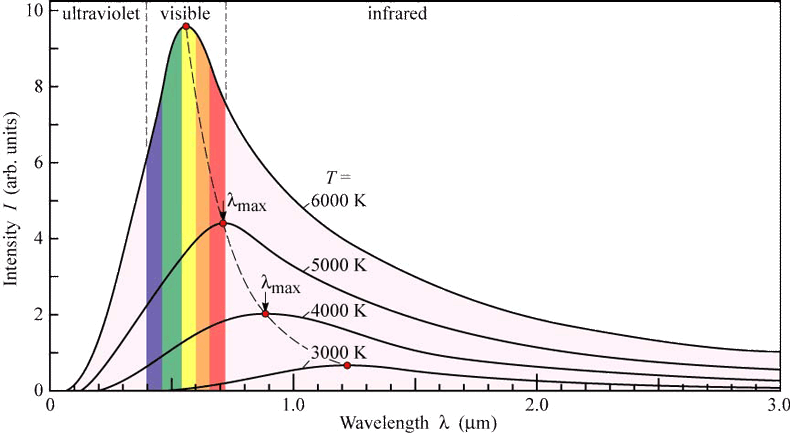
\includegraphics[width=\textwidth]{figures/exampleFigure.png}
	\caption{This is an example Figure.}
	\label{Figure in Chapter 1}
\end{figure}


Lorem ipsum dolor sit amet, consectetur adipiscing elit, sed do eiusmod tempor incididunt ut labore et dolore magna aliqua. Ut enim ad minim veniam, quis nostrud exercitation ullamco laboris nisi ut aliquip ex ea commodo consequat \cite{ref1}. Duis aute irure dolor in reprehenderit in voluptate velit esse cillum dolore eu fugiat nulla pariatur \cite{ref2}. Excepteur sint occaecat cupidatat non proident, sunt in culpa qui officia deserunt mollit anim id est laborum.

Lorem ipsum dolor sit amet, consectetur adipiscing elit, sed do eiusmod tempor incididunt ut labore et dolore magna aliqua. Ut enim ad minim veniam, quis nostrud exercitation ullamco laboris nisi ut aliquip ex ea commodo consequat \cite{ref1}. Duis aute irure dolor in reprehenderit in voluptate velit esse cillum dolore eu fugiat nulla pariatur \cite{ref2}. Excepteur sint occaecat cupidatat non proident, sunt in culpa qui officia deserunt mollit anim id est laborum.

Lorem ipsum dolor sit amet, consectetur adipiscing elit, sed do eiusmod tempor incididunt ut labore et dolore magna aliqua. Ut enim ad minim veniam, quis nostrud exercitation ullamco laboris nisi ut aliquip ex ea commodo consequat \cite{ref1}. Duis aute irure dolor in reprehenderit in voluptate velit esse cillum dolore eu fugiat nulla pariatur \cite{ref2}. Excepteur sint occaecat cupidatat non proident, sunt in culpa qui officia deserunt mollit anim id est laborum.

Lorem ipsum dolor sit amet, consectetur adipiscing elit, sed do eiusmod tempor incididunt ut labore et dolore magna aliqua. Ut enim ad minim veniam, quis nostrud exercitation ullamco laboris nisi ut aliquip ex ea commodo consequat \cite{ref1}. Duis aute irure dolor in reprehenderit in voluptate velit esse cillum dolore eu fugiat nulla pariatur \cite{ref2}. Excepteur sint occaecat cupidatat non proident, sunt in culpa qui officia deserunt mollit anim id est laborum.

Lorem ipsum dolor sit amet, consectetur adipiscing elit, sed do eiusmod tempor incididunt ut labore et dolore magna aliqua. Ut enim ad minim veniam, quis nostrud exercitation ullamco laboris nisi ut aliquip ex ea commodo consequat \cite{ref1}. Duis aute irure dolor in reprehenderit in voluptate velit esse cillum dolore eu fugiat nulla pariatur \cite{ref2}. Excepteur sint occaecat cupidatat non proident, sunt in culpa qui officia deserunt mollit anim id est laborum.

Lorem ipsum dolor sit amet, consectetur adipiscing elit, sed do eiusmod tempor incididunt ut labore et dolore magna aliqua. Ut enim ad minim veniam, quis nostrud exercitation ullamco laboris nisi ut aliquip ex ea commodo consequat \cite{ref1}. Duis aute irure dolor in reprehenderit in voluptate velit esse cillum dolore eu fugiat nulla pariatur \cite{ref2}. Excepteur sint occaecat cupidatat non proident, sunt in culpa qui officia deserunt mollit anim id est laborum.

% This is a table

\begin{table}
\caption{This is an example Table.}
\begin{center}
\begin{tabular}{ccc}
x & f(x) & g(x) \\
\hline
1 & 6 & 4  \\
2 & 6 & 3  \\
3 & 6 & 2  \\
4 & 6 & 2  \\
\label{Table in Chapter 1}
\end{tabular}
\end{center}
\end{table}


%%%%%%%%%%%%%%%%
% Chapter 2
%%%%%%%%%%%%%%%%

\chapter{Hybrid Beam Element Formulation}\label{chapter:CH2}


\section{Introduction}\label{section:CH2-S1}
In this chapter we present the formulation of a
novel hybrid beam element which is based on \acrshort{nlp} principles. The 
kinematic assumptions adopted fall under the category of 
geometrically exact or Simo-Reissner beam 
theory\cite{Reissner1,Simo1,Simo2,Simo3}, whereby no simplifying approximation 
is made with respect to the strain-displacement equations. This allows for 
capturing arbitrarily large displacements and rotations, as well as 
accounting for the effect of shear deformation at the section level. 

As opposed to deriving the system equations
from the Galerkin form, we recast the
problem in an \acrshort{nlp} framework by utilizing the underlying
variational structure. The total potential energy (\acrshort{tpe}) functional 
is augmented with
all relevant conditions that enforce the exact kinematics, by intoducing a set
of Lagrange multipliers that act as conjugate force quantities. The resulting
modified functional is then approximated by employing a Gauss-Legendre 
quadrature
rule, which yields the objective function to be minimized. With this particular
approach, the primary variables in the element interior contributing to the
elastic strain energy are the generalized strain measures of the
centroid, which are the unknown quantities at the quadrature points.
Displacement measures at the edge nodes of the element, namely, the translations
along coordinate axes and the rotation of cross sections, are only
associated with the external work. Kinematic consistency between the rotational
measures of displacement and strains is enforced by using a Lagrange
interpolation scheme for the curvature field, similar to the one
used by Neuenhofer and
Filippou \cite{Neuenhofer} and Schulz \& Filippou \cite{Schulz}
for force-based elements. In this work, the points used for 
the interpolation
coincide with the integration points of the quadrature rule used for 
approximating
the energy functional. To avoid ill-conditioning issues of the 
linearized operator, we also outline a block-elimination procedure for the 
linear system involving the Hessian matrix so that the
reduced system includes only displacement components. The corresponding
stiffness operator is well-conditioned, sparse, banded and symmetric. This 
renders standard \acrshort{fem} routines from existing codes 
reusable and, in conjuction with the capability for accuracy even with crude
discretization, provides an attractive formulation for fast and accurate
computation. Additionally, accuracy and locking free performance are guaranteed
with just one element per structural member, even in the presence of arbitrarily
large displacements and rotations. Accordingly, the element can also capture 
high 
curvature gradients due to plastic hinge formation, in the case of inelastic
analysis.

This chapter starts with a brief outline of the beam geometric description 
while adhering to the derivations by Cardona \& Geradin\cite{Cardona}, followed 
by the hybrid \acrshort{nlp} formulation for the element. The third section is 
devoted to implementation details, where special attention is given to the 
block 
elimination technique used for the reduction of the linear system involving the 
Hessian matrix. Finally, the chapter concludes with a set of numerical examples 
where the focus is the Hybrid \acrshort{nlp} element performance with respect 
to coarse mesh discretizations in nonlinear analysis. 

%%%%%%%%%%%%%%%%%%%%% CHAPTER 2 - SECTION 2 %%%%%%%%%%%%%%%%%%%%%%%%%%%%%%
\section{Geometrically-Exact Model}\label{section:CH2-S2}
%%%%%%%%%%%%%%%%%%%%%%%%%%%%%%%%%%%%%%%%%%%%%%%%%%%%%%%%%%%%%%%%%%%%%%%%%%

%%%%%%%%%%%%%%%%%%%%% CHAPTER 2 - SUBSECTION 1 %%%%%%%%%%%%%%%%%%%%%%%%%%%%%%
\subsection{Beam Kinematics}\label{subsection:CH2-S2SS1}
Let \{$\mathbf{E}$\} be a fixed orthonormal coordinate frame with unit vectors
$\{\bvec{E}_1,\ \bvec{E}_2,\ \bvec{E}_3\}$ along the axes $X_1, X_2, X_3$. For
an initially straight beam of length $\ell$ with its centerline coinciding with
$X_1$, the undeformed configuration is completely described by:
\begin{gather}
	\bvec{X}(X_1,X_2) = X_1\bvec{E}_1 + X_2\bvec{E}_2 =
	\bvec{r}_o(X_1)+\bvec{t}(X_2)
\end{gather}

% ADD UNDEFORMED + DEFORMED SKETCH
\begin{figure}[t]
	\centering
	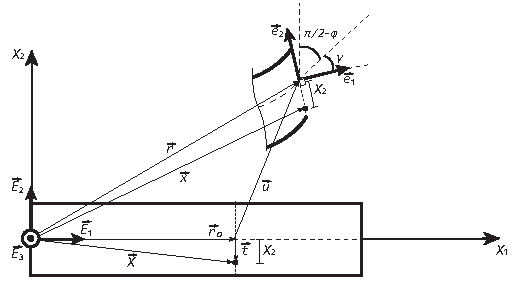
\includegraphics[scale=1.25]{FIG1_BEAM_THEORY}
	\caption{Undeformed and deformed configurations of the beam.}
	\label{fig:FIG1}
\end{figure}

\noindent where $\bvec{r}_o$ traces the centerline in the reference 
configuration
and $\bvec{t}$ locates a material point on the cross section. Assuming a
rectangular cross-section of height $h$, without loss of generality, we have 
that
$X_1\in[0,\ \ell]$ and $X_2\in[-\sfrac{h}{2}, \sfrac{h}{2}]$. We should
note here that $X_3$ is omitted as it does not explicitly come into the
expressions. We nevertheless hold on to the $\mathbb{R}^3$ vector formalism to
maintain consistency with the representation of rotation as a linear operator.
After the application of a displacement field $\bvec{u}(X_1)$, the
deformed configuration is given by vector $\bvec{x}$ such that:
\begin{gather}
	\bvec{r} = \bvec{r}_o + \bvec{u} \label{eq:def1}\\
	\bvec{x}=\bvec{r} + X_2\bvec{e}_2 \label{eq:deformed}
\end{gather}

\noindent where $\{\mathbf{e}\}$ is a local coordinate system attached at
cross-sections that completely describes their orientation. For the unit vectors
of the local base $\bvec{e}_1,\ \bvec{e}_2,\ \bvec{e}_3$, we let $\bvec{e}_1$ be
normal to the cross-section, but not necessarily tangent to the deformed
centerline, and $\bvec{e}_2$ (and $\bvec{e}_3$) coincide with the cross-section
principal axes of inertia, as shown in Fig. \ref{fig:FIG1}.

If $\bmat{R}$ is the rotation operator that rotates $\{\mathbf{E}\}$ to
$\{\mathbf{e}\}$, then:
\begin{gather}
	\bvec{e}_i = \bmat{R}\bvec{E}_i ,\quad i=1,2,3
	\label{eq:roteq}
\end{gather}

\noindent For the plane case, the component form of $\bmat{R}$ reduces to:
\begin{gather}
	\bmat{R} = \begin{bmatrix}
		\cos\phi &-\sin\phi & 0\\
		\sin\phi &\cos\phi & 0\\
		0 & 0 & 1
	\end{bmatrix}
\end{gather}

\noindent Then, using Eq. (\ref{eq:roteq}), Eq. (\ref{eq:deformed}) becomes:
\begin{gather}
	\bvec{x} = \bvec{r} + \bmat{R}\bvec{t}
	\label{eq:deformed1}
\end{gather}

\noindent For Eqs. (\ref{eq:deformed}),(\ref{eq:deformed1}) to hold in this
manner, we tacitly assume that cross-sections remain rigid during
deformation, that is, the position of a material point on a cross-section
with respect to the centroid does not change.


%%%%%%%%%%%%%%%%%%%%% CHAPTER 2 - SUBSECTION 2 %%%%%%%%%%%%%%%%%%%%%%%%%%%%%%
\subsection{Strain Measures, Strain-Displacement
Relations}\label{subsection:CH2-S2SS2}
Within the context of geometrically-exact formulations, it is common to adopt as
a strain measure $\bvec{s}$ the difference of the position vector gradients,
$\bvec{r}$ and $\bvec{r}_o$, with respect to the local frame (e.g. see
\cite{Simo1,Cardona,Hodges}). Denoting derivatives with respect to $X_1$
by $(\cdot)'$, we get:			% HERE
\begin{gather}
	\bvec{s} = \bmat{R}^T\bvec{r}'- \bvec{r}'_o
	\label{eq:strm}
\end{gather}

\noindent whereas the cross-section curvature is given as:
\begin{gather}
	\kappa=\phi'
	\label{eq:kapa}
\end{gather}

\noindent The axial and shear strain of the centroid, $\epsilon$ and
$\gamma$ respectively, can then be retained as follows:
\begin{gather}
	\epsilon = \bvec{e}_1^T\bvec{s}\\
	\gamma = \bvec{e}_2^T\bvec{s}
\end{gather}

\noindent where $\bvec{s}=\begin{bmatrix}
	\epsilon & \gamma & 0
\end{bmatrix}^T$, with the third component, representing the shear strain along
the out-of-plane axis, being by assumption zero.

Using Eq. (\ref{eq:def1}) and performing the differentiations in
Eq. (\ref{eq:strm}) with respect to $X_1$, we get:
\begin{gather}
	\bvec{s} = \bmat{R}^T[\bvec{u}'+\bvec{E}_1] - \bvec{E}_1
	\label{eq:strd}
\end{gather}

\noindent Deriving the exact differential strain-displacement relations as
presented in Reissner\footnote{See equations (15) in \cite{Reissner1}} is 
straigtforward if we solve Eq. (\ref{eq:strd}) for $\bvec{u}'$:
\begin{gather}
	\bvec{u}' = \bmat{R}\bvec{s}+\bvec{e}_1-\bvec{E}_1
	\label{eq:reissd}
\end{gather}

\noindent If we write $\bvec{u} = \begin{bmatrix} u & v & 0
\end{bmatrix}^T$, then the explicit expressions for $u',v'$ along with
Eq. (\ref{eq:kapa}) are:
\begin{subequations}
	\begin{gather}
		u'= \bvec{E}_1^T\bvec{u}'=(1+\epsilon)\cos\phi-\gamma\sin\phi-1\\
		v'= \bvec{E}_2^T\bvec{u}'=(1+\epsilon)\sin\phi+\gamma\cos\phi\\
		\phi'=\kappa\label{eq:cond3}
	\end{gather}
\end{subequations}

\noindent By introducing vectors $\bvec{d}$ and $\bvec{q}$, such that $
\bvec{d} = \begin{bmatrix}
	u & v & \phi
\end{bmatrix}^T $ and $ \bvec{q} = \begin{bmatrix}
	\epsilon & \gamma & \kappa
\end{bmatrix}^T$, we can maintain the structure of Eq. (\ref{eq:reissd}) and
express all fields involved in matrix notation, as follows:
\begin{gather}
	\bvec{d}' = \bmat{R}\bvec{q}+\bvec{e}_1-\bvec{E}_1
	\label{eq:mainsd}
\end{gather}

\noindent Strain-displacement equations as represented in Eq. (\ref{eq:mainsd})
will be subsequently utilized in the formulation of the beam model.

%%%%%%%%%%%%%%%%%%%%% CHAPTER 2 - SECTION 3 %%%%%%%%%%%%%%%%%%%%%%%%%%%%%%
\section{Nonlinear Programming Formulation of the Hybrid Beam 
Element}\label{section:CH2-S3}
%%%%%%%%%%%%%%%%%%%%%%%%%%%%%%%%%%%%%%%%%%%%%%%%%%%%%%%%%%%%%%%%%%%%%%%%%%

The hybrid beam element discretization is presented by utilizing the underlying
variational structure of the static problem. The minimizing principle for the
\acrshort{tpe} is recast here in an \acrshort{nlp}
formulation and the strain-displacement equations in (\ref{eq:mainsd}) are
incorporated, representing the equality constraints of the problem.

%%%%%%%%%%% CHAPTER 2 - SECTION 3 -S UBSECTION 1%%%%%%%%%%%%
\subsection{NLP Framework}\label{subsection:CH2-S3SS1}

The \acrshort{nlp} problem adopted herein is of the following form:
\begin{align}
	&\text{minimize} \hspace{1cm}f(\bvec{x})\nonumber\\
	&\text{subject to}\hspace{1.cm}  \bvec{h}(\bvec{x})=\bvec{0}\label{eq:nlp}\\
	&\hspace{2.4cm} \bvec{x}\in\mathcal{S}\nonumber
\end{align}

\noindent The objective function $f(\bvec{x})$ represents the total potential
energy of the structure, whereas vector $\bvec{h}(\bvec{x})$ includes the active
constraints of the program. The corresponding Lagrangian is:
\begin{gather}
	\mathcal{L}(\bvec{x},\bvec{\lambda}) = f(\bvec{x}) + 
	\bvec{\lambda}^T\bvec{h}(\bvec{x})
	\label{eq:lagr}
\end{gather}
\noindent where $\bvec{\lambda}$ are the Lagrange multipliers. The first-order
optimality conditions are given from the following expression:
\begin{gather}
	\nabla\mathcal{L}=\bvec{0}
	\label{eq:gradz}
\end{gather}

\noindent This is the standard form of a nonlinear constrained minimization
program with equality constraints, as encountered in the literature (e.g. 
\cite{Luenberger}).

%%%%%%%%%%% CHAPTER 2 - SECTION 3 -S UBSECTION 2 %%%%%%%%%%%%
\subsection{Discretization of Total Potential 
Energy}\label{subsection:CH2-S3SS2}

We consider the following decomposition of the total potential energy of a beam:
\begin{gather}
	\Pi = U - W
	\label{eq:tpe1}
\end{gather}

\noindent where $U$ and $W$ are the stored strain energy and potential energy
associated with external loading respectively. For the case of concentrated
external loads, Eq. (\ref{eq:tpe1}) can be expressed as:
\begin{gather}
	\Pi = \int_0^\ell\ \mathcal{W}_S(X_1,\bvec{q})\ dX_1 - 
	\sum_{i=1}^2\bvec{P}_i^T\bvec{u}_i
	\label{eq:tpe2}
\end{gather}

\noindent where $\mathcal{W}_S$ is the strain energy density of a cross section
at $X_1$ and $\bvec{q}$ denotes the neutral axis strain vector, 
$\bvec{P}_i$,$\bvec{u}_i$ the element nodal force and
displacement vectors, respectively. It can be proven\cite{Washizu} that for 
strain hardening materials
within the premises of small strain elastoplasticity, the exact solution to the 
problem renders $\Pi$ an absolute minimum.
Equivalently, the exact solution solves the program
in Eq. (\ref{eq:nlp}) for $f=\Pi$ with $\bvec{h}$ acting as constraints.
Assuming a stable
work-hardening material, the corresponding Euler-Lagrange equations yield the
constitutive equations of elastoplasticity (e.g. see discussion in Simo and 
Hughes
\cite{SimoHughes}). As it will be shown in subsequent sections, since the
constitutive update is carried out locally at the section fiber level.

Section stress
resultants are then given by the gradient of $\mathcal{W}_S$:
\begin{gather}
	\bvec{F}_{sec} = \nabla_{\mathbf{q}} \mathcal{W}_S
\end{gather}
with $\bvec{F}_{sec} = \begin{bmatrix} N & V & M \end{bmatrix}^T$.
\noindent In the case of linear elasticity, the energy density is
given by $\mathcal{W}_S = \frac{1}{2}[ EA\epsilon^2 + GA_s\gamma^2 +
EI\kappa^2]$  and the section resultants are:
\begin{gather*}
	\bvec{F}_{sec} = \begin{bmatrix}
		EA\epsilon\\
		GA_s\gamma\\
		EI\kappa
	\end{bmatrix}
\end{gather*}

\noindent where $A_s$ is the effective shear area of the cross-section. 
Numerical
approximation of Eq. (\ref{eq:tpe2}) by an appropriate quadrature yields:
\begin{gather}
 	\Pi(\bvec{q}_1,\ldots,\bvec{q}_n,\bvec{u}_1,\ldots\bvec{u}_N) = 
 	\sum_{i=1}^{n_q}
	w_i\mathcal{W}_{S,i} - \sum_{i=1}^2\bvec{P}^T_i\bvec{u}_i
	\label{eq:obj}
\end{gather}

\noindent with $w_i$ and $n_q$ being the weights and the number of 
integration
points respectively, and $\mathcal{W}_{S,i} = \mathcal{W}_S(\bvec{q}_i)$.
Eq. (\ref{eq:obj}) serves as the objective function of the \acrshort{nlp} of
Eq. (\ref{eq:nlp}).

%%%%%%%%%%% CHAPTER 2 - SECTION 3 - SUBSECTION 3 %%%%%%%%%%%%
\subsection{Discretization of Strain-Displacement 
Relations}\label{subsection:CH2-S3SS3}

The constrained conditions are derived by applying the same quadrature rule on
the integral form of the strain-displacement equations (\ref{eq:mainsd}):
\begin{gather}
	\bvec{d}(\ell)-\bvec{d}(0) = \int_0^\ell\ \bvec{d}'\ dX_1=\int_0^\ell\
	\bmat{R}\bvec{q}+\bvec{e}_1-\bvec{E}_1\ dX_1
	\label{eq:cintform}
\end{gather}

\noindent Using Eq. (\ref{eq:roteq}), numerical approximation of the right-hand
side integral leads to the element specific constraints:
\begin{gather}
	\bvec{h}^A = \bvec{d}(\ell)-\bvec{d}(0) - \sum_{i=1}^{n_q}
	w_i\bmat{R}_i(\bvec{q}_i+\bvec{E}_1)+\ell\bvec{E}_1=\bvec{0}
	\label{eq:dsd}
\end{gather}


\noindent The component form of Eq. (\ref{eq:dsd}) can be given as:
\begin{gather}
	\bvec{h}^A = \begin{bmatrix}
		u(\ell)-u(0) - \sum_{i=1}^{n_q} 
		w_i\bigg[(\epsilon_i+1)\cos\phi_i -
		\gamma_i\sin\phi_i\bigg] +\ell\\
		v(\ell)-v(0) - \sum_{i=1}^{n_q} 
		w_i\bigg[(\epsilon_i+1)\sin\phi_i +
		\gamma_i\cos\phi_i\bigg]\\
		\phi(\ell)-\phi(0) - \sum_{i=1}^{n_q} w_i\kappa_i
	\end{bmatrix}
\end{gather}

Although the strain fields appear explicitly
only in the weighted evaluation points of the quadrature, the rotational field
$\phi$ is involved in both the integration points and the element edge nodes.
As such, we introduce a Lagrange interpolation scheme for the curvature
field in the same fashion as in \cite{Andriotis}:
\begin{equation}
	\kappa(\xi) = \sum_{i=1}^{n_q}L_i(\xi)\kappa_i
	\label{eq:curvi}
\end{equation}

\noindent where $L_i$ are the Lagrange cardinal functions:
\begin{equation}
	L_i(\xi) = \frac{\displaystyle\prod_{j=1,j\neq i}^{n_q}
		(\xi-\xi_j)}{\displaystyle\prod_{j=1,j\neq i}^{n_q} 
		(\xi_i-\xi_j)}\text{,}\quad
	\xi=\frac{X_1}{\ell}\nonumber
\end{equation}

\noindent Substitution of Eq. (\ref{eq:curvi}) to Eq. (\ref{eq:cond3}) yields
the expression for rotations $\phi_i$:
\begin{equation}
	\phi_i-\phi(0) = \sum_{j=1}^{n_q}\bigg(\int_0^{\xi_i}L_j(x)\ 
	dx\bigg)\kappa_j =
	\sum_{i=1}^{n_q} T_{ij}\kappa_j
\end{equation}
\begin{figure*}[b]
	\centering
	\subfloat{{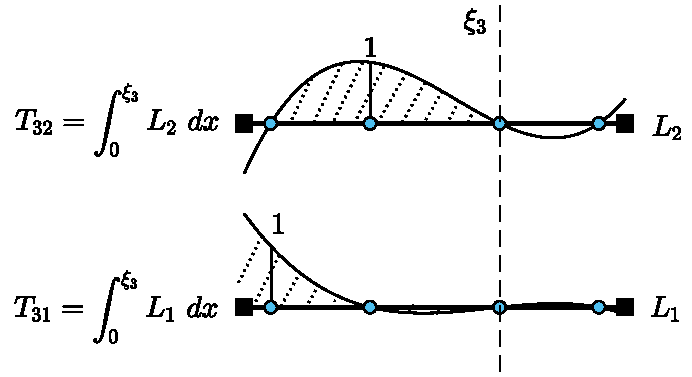
\includegraphics[width=7cm]{FIG2_A.pdf} }}%
	\qquad
	\subfloat{{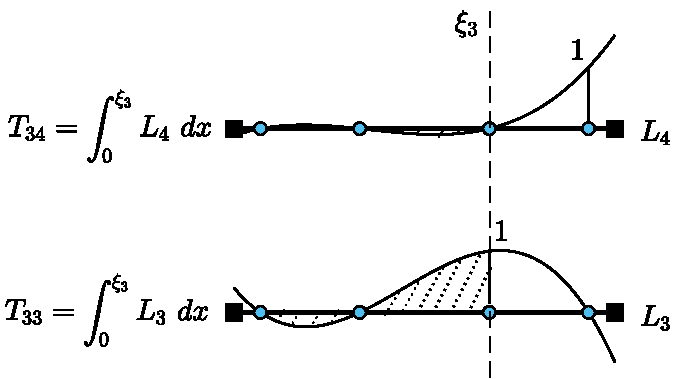
\includegraphics[width=7cm]{FIG2_B.pdf} }}%
	\caption{Integration of curvature shape functions.}%
	\label{fig:fig2}%
\end{figure*}
\noindent with derivation of $T_{ij}$ illustrated in Fig.  \ref{fig:fig2}.
In matrix form, the above equation can be directly restated as a linear
equality constraint set as:
\begin{equation}
	\bvec{h}^B=\bvec{\phi} - \phi(0)\bvec{1} - \bmat{T}\bvec{\kappa} = \bvec{0}
	\label{eq:hb}
\end{equation}

\noindent where
\begin{gather}
	\bvec{\phi}=
	\begin{bmatrix}
		\phi_1 & \phi_2 & \cdots & \phi_{n_q}
	\end{bmatrix}^T\quad \text{,}\ \bvec{1}= \begin{bmatrix}
		1 & 1 & \cdots & 1
	\end{bmatrix}^T\in\mathbb{R}^{n_q} \nonumber\\
	\bmat{T} = L\begin{bmatrix}
		\xi_1 & \frac{\xi_1^2}{2} & \cdots & 
		\frac{\xi_1^{n_q}}{n_q}\\
		\vdots & \vdots & \ddots & \vdots\\
		\xi_{n_q} & \frac{\xi_{n_q}^2}{2} & \cdots & 
		\frac{\xi_{n_q}^{n_q}}{n_q}
	\end{bmatrix}\bmat{\Theta}^{-1}\quad \text{,}\ \bmat{\Theta} = 
	\begin{bmatrix}
		1 & \xi_1 & \xi_1^2 & \cdots & \xi_1^{n_q-1}\\
		\vdots &\vdots & \ddots & \vdots\\
		1 & \xi_{n_q} & \xi_{n_q}^2 & \cdots &\xi_{n_q}^{n_q-1}
	\end{bmatrix}\nonumber
\end{gather}

\noindent We can then collect all active constraints, Eqs.
(\ref{eq:dsd}),(\ref{eq:hb}), in one vector $\bvec{h}$:
\begin{equation}
	\bvec{h} = \begin{bmatrix}
		\bvec{h}^A \\
		\bvec{h}^B
	\end{bmatrix} = \begin{bmatrix}
		\bvec{0}\\
		\bvec{0}
	\end{bmatrix}
	\label{eq:constr}
\end{equation}

\noindent containing all constraints pertaining to one element.
While vector $\bvec{h}^A$ of strain-displacement constraints
will always contain three components for each element, the number of components 
in vector
$\bvec{h}^B$ will depend on the chosen quadrature rule.

%%%%%%%%%%% CHAPTER 2 - SECTION 3 - SUBSECTION 4 %%%%%%%%%%%%
\subsection{Lagrangian Function for the Structure}\label{subsection:CH2-S3SS4}

In order to derive the Lagrangian function in the form of Eq. (\ref{eq:lagr}),
we introduce a vector $\bvec{\lambda}$ of additional Lagrange multiplier
variables and augment Eq. (\ref{eq:obj}) with Eq. (\ref{eq:constr}):  % HERE
\begin{gather}
	\mathcal{L} = f + \bvec{\lambda}^T\bvec{h}
	\label{eq:elangr}
\end{gather}

\noindent A more convenient form for the Lagrangian function can also be
achieved by expanding $f$ into its constituents, namely, the element stored
energy and the potential energy:
\begin{gather}
	\mathcal{L} = \sum_{e=1}^{n_{el}}U^e - W +
	\bvec{\lambda}^T\bvec{h}
	\label{eq:langrT}
\end{gather}

\noindent where:
\begin{gather}
	U^e = \sum_{i=1}^{n_q} w_i\mathcal{W}_{S,i}^e \quad 
	\text{,}\quad W = 
	\sum_{i=1}^{N_{nod}}
	\bvec{P}_i^T\bvec{u}_i\nonumber
\end{gather}

\noindent where $N_{nod}$ is the total number of nodes in the 
structure. Thereby, additional elements can be simply incorporated 
by adding
their stored energy in the corresponding sum, and considering element
constraints by augmenting vectors $\bvec{\lambda}$, $\bvec{h}$, after 
transforming
them to the global system. Potential function $W$ is ``global" in the
sense that external loads and the corresponding work-conjugate displacement
degrees of freedom are directly added to the expression and are not
influenced by adding nodal contributions from adjacent elements. As a result,
no additional connectivity constraints at the element interfaces are needed,
and Eq. (\ref{eq:langrT}) is thus a global function for the
whole structure.


%%%%%%%%%%%%%%%%%%%%% CHAPTER 2 - SECTION 4 %%%%%%%%%%%%%%%%%%%%%%%%%%%%%%
\section{Implementation}\label{section:CH2-S4}
%%%%%%%%%%%%%%%%%%%%%%%%%%%%%%%%%%%%%%%%%%%%%%%%%%%%%%%%%%%%%%%%%%%%%%%%%%

The set of vectors associated with internal field variables,
$\{\bvec{y}_i\}_{i=1}^n$, is defined as $\bvec{y}_i =\begin{bmatrix}
	\bvec{q}_i & \phi_i
\end{bmatrix}^T= \begin{bmatrix}
	\epsilon_i & \gamma_i & \kappa_i & \phi_i
\end{bmatrix}^T$. Moreover, and according to Fig. \ref{fig:fig3}, we designate
the local element edge degrees of freedom in vector form as
$\bhat{d}_l = \bvec{d}(0)$ and $\bhat{d}_r = \bvec{d}(\ell)$. The element 
displacement
vector is thus $\bhat{d} = \begin{bmatrix} \bhat{d}_l^T & \bhat{d}_r^T 
\end{bmatrix}^T$. The corresponding
global displacement vector $\bvec{d}_g$ is related to the local 
vector
$\bhat{d}$ via the typical linear transformation $\bmat{\Lambda}$:  % HERE

\begin{gather}
	\bhat{d} = \begin{bmatrix}
		\bmat{\Lambda} & \bmat{0}\\
		\bmat{0} & \bmat{\Lambda}
	\end{bmatrix}\bvec{d}_g
	\quad\text{,}\quad \bmat{\Lambda}=\begin{bmatrix}
		\cos\theta & \sin\theta & 0\\
		-\sin\theta & \cos\theta & 0\\
		0 & 0 & 1
	\end{bmatrix}
\end{gather}

\begin{figure}[b]
	\centering
	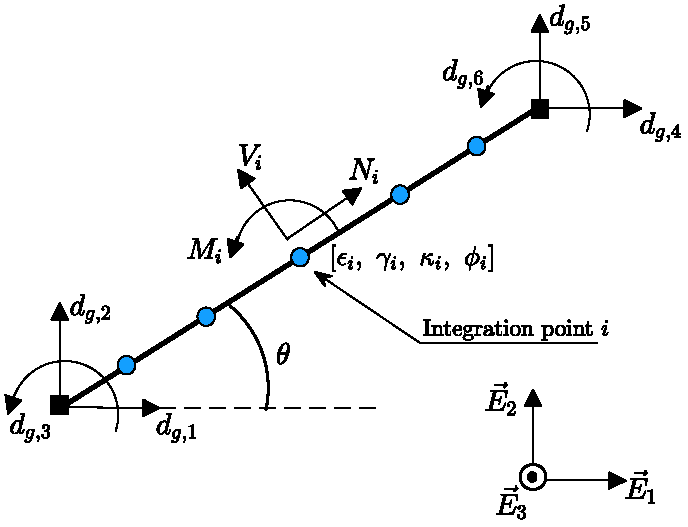
\includegraphics[width=0.45\textwidth]{FIG3_ELEMENT.pdf}
	\caption{Typical element representing one member.}
	\label{fig:fig3}
\end{figure}

\noindent The element constraints of Eqs. (\ref{eq:dsd}),(\ref{eq:hb})
transformed in the global system become:  % HERE
\begin{subequations}
	\begin{gather}
		\bvec{h}^A_g = \bmat{V}_1\bvec{d}_g - 
		\bmat{\Lambda}^T\bigg[\sum_{i=1}^{n_q}
		w_i\bmat{R}_i(\bvec{q}_i+\bvec{E}_1) - \ell\bvec{E}_1\bigg]
		\label{eq:impsd1}\\
		\bvec{h}^B_g = \bvec{\phi}-\bmat{V}_2\bvec{d}_g - \bmat{T}\bvec{\kappa}
		\label{eq:impsd2}
	\end{gather}
\end{subequations}

\noindent where:
\begin{gather}
	\bmat{V}_1 = \begin{bmatrix}
		-\bmat{I} & \bmat{I}
	\end{bmatrix}\quad\text{,}\quad
	\bmat{V}_2 = \begin{bmatrix}
		\bvec{0} & \bvec{0} & \bvec{1} & \bvec{0} & \bvec{0} & \bvec{0}
	\end{bmatrix}\nonumber\\
	\bmat{I} = \begin{bmatrix}
		1 & 0 & 0\\
		0 & 1 & 0\\
		0 & 0 & 1
	\end{bmatrix}\quad\text{,}\quad 
	\bvec{0}\in\mathbb{R}^{n_q}\nonumber
\end{gather}

\noindent In the equation above the superscript denoting an element is omitted
for clarity. The element contribution to the Lagrangian of the assemblage,
denoted $\mathcal{E}^e$, is then:
\begin{gather}
	\mathcal{E}^e(\bvec{y}_1,\dots \bvec{y}_{n_q}, 
	\bvec{d}_g,\bvec{\lambda}^e) =
	U^e  + (\bvec{\lambda}^e)^T\bvec{h}^e_g
	\label{eq:implag}
\end{gather}

\noindent Notice that the external potential function $W$ is not included
in Eq. (\ref{eq:implag}) as it is added directly via the work done by external
forces in the global degrees of freedom and not from element contributions.
The element Lagrange multipliers $\bvec{\lambda}^e$ are force
conjugate measures at the corresponding degrees of freedom and $U^e$ is the
sum total of cross-section strain energies.
The Lagrangian of the whole system is accordingly given by:
\begin{gather}
	\mathcal{L}(\bvec{y}, \bvec{d}_g,\bvec{\lambda}) =
	U-W+\bvec{\lambda}^T\bvec{h}_g
	%\label{eq:globalL}
\end{gather}
\noindent which is a restatement of Eq. (\ref{eq:langrT}) in the global 
coordinate
system and $\bvec{y} = \begin{bmatrix}
	\bvec{y}_1^T & \bvec{y}_2^T & \cdots & \bvec{y}_m^T
\end{bmatrix}^T$, with $m$ being the total number of quadrature points in
the structure.

%%%%%%%%%%% CHAPTER 2 - SECTION 4 - SUBSECTION 1 %%%%%%%%%%%%
\subsection{Optimality Conditions as Structural Equilibrium Equations 
}\label{subsection:CH2-S4SS1}

In what follows, it is assumed we are dealing with quantities pertaining to
the total assemblage, after all element contributions have been resolved.
The first-order necessary optimality condition for the Lagrangian function (see 
Eq.
(\ref{eq:gradz})), after the imposition of boundary conditions, yields the
following relations:
\begin{subequations}
	\begin{gather}
		\nabla_{\mathbf{y}_i}\mathcal{L} = \nabla_{\mathbf{y}_i}U +
		[\nabla_{\mathbf{y}_i}\bvec{h}_g]\bvec{\lambda} = 
		\bvec{0}\label{eq:g1}\\
		\nabla_{\mathbf{d}_g}\mathcal{L} = -\nabla_{\mathbf{d}_g}W +
		[\nabla_{\mathbf{d}_g}\bvec{h}_g]\bvec{\lambda} = 
		\bvec{0}\label{eq:g2}\\
		\nabla_{\mathbf{\lambda}}\mathcal{L} = \bvec{h}_g = 
		\bvec{0}\label{eq:g3}
	\end{gather}\label{eq:eqtot}
\end{subequations}

\noindent Eq. (\ref{eq:g1}) expresses the equilibrium between external and
internal forces acting on the $i$-th cross-section for $i=1,2,\dots m$,
while Eq.
(\ref{eq:g2}) ensures consistency between externally applied loads and Lagrange
multipliers. Finally, Eq. (\ref{eq:g3}) requires that all constraints are
active when the minimum is attained. Explicit expressions for the first and
second derivatives of all quantities involved are given in the Appendix. We
should note that derivatives of the strain energy $U$ are computed
numerically during the \emph{cross-section state determination} phase in Sec.
(\ref{subsection:CH2-S4SS4}).

%%%%%%%%%%% CHAPTER 2 - SECTION 4 - SUBSECTION 2 %%%%%%%%%%%%
\subsection{The Hessian Matrix}\label{subsection:CH2-S4SS2}

The Hessian matrix of the Lagrangian function contains second order
information of the system and is utilized during the solution phase.
Eqs. (\ref{eq:g1})-(\ref{eq:g3}) constitute a set of nonlinear algebraic
equations and an iterative scheme is needed to solve the system. In block
matrix form, the Hessian is provided as:
\begin{gather}
	\bmat{H} = \begin{bmatrix}
		\nabla^2_{\mathbf{yy}}\mathcal{L} & \nabla^2_{\mathbf{y d_g}}\mathcal{L}
		&\nabla^2_{\mathbf{y\lambda}}\mathcal{L} \\
		\nabla^2_{\mathbf{y d_g}}\mathcal{L}^T  & 
		\nabla^2_{\mathbf{d_gd_g}}\mathcal{L} &
		\nabla^2_{\mathbf{d_g\lambda}}\mathcal{L}\\
		\nabla^2_{\mathbf{y\lambda}}\mathcal{L}^T
		&\nabla^2_{\mathbf{d_g\lambda}}\mathcal{L}^T
		&\nabla^2_{\mathbf{\lambda\lambda}}\mathcal{L}
	\end{bmatrix} = \begin{bmatrix}
		\nabla^2_{\mathbf{yy}}\mathcal{L} & \bmat{0} & 
		\nabla_{\mathbf{y}}\bvec{h}^T_g\\
		\bmat{0} & \bmat{0} & \nabla_{\mathbf{d_g}}\bvec{h}^T_g\\
		\nabla_{\mathbf{y}}\bvec{h}_g & \nabla_{\mathbf{d_g}}\bvec{h}_g & 
		\bmat{0}\\
	\end{bmatrix}
	\label{eq:hess}
\end{gather}

\noindent The resulting Hessian is fairly sparse. Moreover, the block
matrix $\nabla_{\mathbf{yy}}U$ which contains section stiffness information is
block-diagonal (see Appendix \ref{appendix:B}) and its
symmetry guarantees the full symmetry of $\bmat{H}$.

%%%%%%%%%%% CHAPTER 2 - SECTION 4 - SUBSECTION 3 %%%%%%%%%%%%
\subsection{Linearization of Equilibrium Equations}\label{subsection:CH2-S4SS3}

As mentioned in Appendix \ref{appendix:B}, the nonlinear system of equations in 
Eq.
(\ref{eq:gradz}) is solved in an incremental-iterative fashion. Linearization 
around
the current iteration $k$ yields:
\begin{gather}
	\nabla\mathcal{L}^k + \bmat{H}^k\delta\bvec{z}^k = \bvec{0}
	\label{eq:linsys}
\end{gather}
\noindent where $\bvec{z}$ is the vector of \emph{all} unknowns:
\begin{gather*}
	\bvec{z} = \begin{bmatrix}
		\bvec{y}\\
		\bvec{d}_g\\
		\bvec{\lambda}
	\end{bmatrix},\quad\text{with}\quad \bvec{y} = \begin{bmatrix}
		\bvec{y}_1\\
		\vdots\\
		\bvec{y}_m
	\end{bmatrix}
\end{gather*}
Reference to the current iteration step is omitted subsequently
for clarity.
Solving Eq. (\ref{eq:linsys}) directly may be cumbersome in
some cases, especially for problems that require denser distribution of
integration points (e.g. plasticity), since the Hessian is not banded and
may also be badly conditioned. In addition, implementation of
continuation schemes in order to attain solutions past critical points
is more involved since the state variable vector contains displacements, strains
and Lagrange multiplier unknowns. A different approach is hence sought,
where the initial linear system is reduced to a smaller one involving only the
displacement vector $\bvec{d}_g$. Restating the system in terms of its
distinct vector components $\bvec{y}$, $\bvec{d}_g$ and $\bvec{\lambda}$
gives:
\begin{gather}
	\begin{bmatrix}
		\nabla_{\mathbf{y}}\mathcal{L}\\
		\nabla_{\mathbf{d}_g}\mathcal{L}\\
		\nabla_{\mathbf{\lambda}}\mathcal{L}
	\end{bmatrix} +
	\begin{bmatrix}
		\nabla^2_{\mathbf{yy}}\mathcal{L} & \bmat{0} & 
		\nabla_{\mathbf{y}}\bvec{h}^T_g\\
		\bmat{0} & \bmat{0} & \nabla_{\mathbf{d}_g}\bvec{h}^T_g\\
		\nabla_{\mathbf{y}}\bvec{h}_g & \nabla_{\mathbf{d}_g}\bvec{h}_g & 
		\bmat{0}\\
	\end{bmatrix}\begin{bmatrix}
		\delta\bvec{y} \\ {\ }\delta\bvec{d}_g \\ \delta\bvec{\lambda}
	\end{bmatrix}
	= \begin{bmatrix}
		\bvec{0}\\ \bvec{0}\\ \bvec{0}
	\end{bmatrix}
	\label{eq:linon}
\end{gather}

\noindent Utilizing Eqs. (\ref{eq:g1})-(\ref{eq:g3}) and setting
$\delta{\bvec{\lambda}} = \bvec{\lambda}^{k+1} - \bvec{\lambda}^k$, Eq.
(\ref{eq:linon}) can be rewritten as:
\begin{gather}
	\begin{bmatrix}
		\nabla_{\mathbf{y}}U\\
		-\bvec{P}\\
		\bvec{h}_g
	\end{bmatrix} +
	\begin{bmatrix}
		\nabla^2_{\mathbf{yy}}\mathcal{L} & \bmat{0} & 
		\nabla_{\mathbf{y}}\bvec{h}^T_g\\
		\bmat{0} & \bmat{0} & \nabla_{\mathbf{d}_g}\bvec{h}^T_g\\
		\nabla_{\mathbf{y}}\bvec{h}_g & \nabla_{\mathbf{d}_g}\bvec{h}_g & 
		\bmat{0}\\
	\end{bmatrix}\begin{bmatrix}
		\delta\bvec{y} \\ {\ }\delta\bvec{d}_g \\ \bvec{\lambda}_{k+1}
	\end{bmatrix}
	= \begin{bmatrix}
		\bvec{0}\\ \bvec{0}\\ \bvec{0}
	\end{bmatrix}
	\label{eq:linprop}
\end{gather}
\noindent As mentioned previously, the gradient of the strain energy with
respect to the strain vector represents the cross-sectional
stress resultants. Solving the
first equation in the system of Eq. (\ref{eq:linprop}) for $\delta\bvec{y}$ we
get:
\begin{gather}
	\delta\bvec{y} =
	-\nabla^2_{\mathbf{yy}}\mathcal{L}^{-1}\bigg[\bvec{F}_{sec}
	+\nabla_{\mathbf{y}}\bvec{h}_g^T\bvec{\lambda}_{k+1}  \bigg]
	\label{eq:e1}
\end{gather}

\noindent Substituting Eq. (\ref{eq:e1}) in the third equation of Eq.
(\ref{eq:linprop}) and solving for $\bvec{\lambda}^{k+1}$ yields: % HERE
\begin{gather}
	\bvec{\lambda}^{k+1} = \bmat{B}^{-1}[\bvec{h}_g -
	\bvec{b}]+\bmat{B}^{-1}[\nabla_{\mathbf{d}_g}\bvec{h}_g]\delta\bvec{d}_g
	\label{eq:e3}
\end{gather}

\noindent By substituting Eq. (\ref{eq:e3}) into the second system equation
Eq.  (\ref{eq:g2}) we arrive at the familiar static equilibrium form of
the system of equations: % HERE
\begin{gather}
	\bmat{K}\delta\bvec{d}_g = \bvec{P} - \bvec{F}_{int}
	\label{eq:stiffsys}
\end{gather}

\noindent which can now be solved for the iterative displacement vector
$\delta\bvec{d}_g$. Vectors $\bvec{b}$, $\bvec{F}_{int}$ and matrices
$\bmat{B}$, $\bmat{K}$, are given by the following explicit formulas
in the global system:
\begin{subequations}
	\begin{align}
		&\bvec{b}
		=[\nabla_{\mathbf{y}}\bvec{h}_g][\nabla^2_{\mathbf{yy}}\mathcal{L}]^{-1}\bvec{F}_{sec}\label{eq:sub1}\\
		&\bvec{F}_{int} =
		[\nabla_{\mathbf{d}_g}\bvec{h}_g]^T[\bmat{B}]^{-1}[\bvec{h}_g-\bvec{b}]\label{eq:sub2}\\
		&\bmat{B}
		=[\nabla_{\mathbf{y}}\bvec{h}_g][\nabla^2_{\mathbf{yy}}\mathcal{L}]^{-1}[\nabla_{\mathbf{y}}\bvec{h}_g]^T
		 \label{eq:sub3}\\
		&\bmat{K}
		=[\nabla_{\mathbf{d}_g}\bvec{h}_g]^T[\bmat{B}]^{-1}[\nabla_{\mathbf{d}_g}\bvec{h}_g]\label{eq:sub4}
	\end{align}
\end{subequations}

\noindent where $\bvec{b}\in\mathbb{R}^p$, 
$\bvec{F}_{int}\in\mathbb{R}^{3N_{nod}}$,
$N_{nod}$ is again the number of structural nodes,
$\bmat{B}\in\mathbb{R}^{p\times p}$ with $p=m+3n_{nel}$, and
$\bmat{K}\in\mathbb{R}^{3N_{nod}\times 3N_{nod}}$. 

Equivalently, an
assembly process can also be implemented by casting 
Eqs. (\ref{eq:sub1}), (\ref{eq:sub3}) in local form, where they can be further 
simplified by being expanded in terms of element cross-section contributions:
\begin{subequations}
	\begin{align}
		\bvec{b}^e&=\sum_{i=1}^{n_q}
		[\nabla_{\mathbf{y}_i}\bvec{h}_g][\nabla^2_{\mathbf{y}_i\mathbf{y}_i}\mathcal{L}]^{-1}\bvec{F}_{sec}^{(i)}\label{eq:subb}\\
		\bmat{B}^e &= \sum_{i=1}^{n_q}
		[\nabla_{\mathbf{y}_i}\bvec{h}_g][\nabla^2_{\mathbf{y}_i\mathbf{y}_i}\mathcal{L}]^{-1}[\nabla_{\mathbf{y}_i}\bvec{h}_g]^T\label{eq:subB}
	\end{align}
\end{subequations}


\noindent where $n$ is the number of element quadrature points,
$\bvec{b}^e\in\mathbb{R}^{n_q+3}$ and 
$\bmat{B}^e\in\mathbb{R}^{(n_q+3)\times 
(n_q+3)}$. 
The element stiffness matrix $\bmat{K}^e\in\mathbb{R}^{6\times 6}$ and 
internal force vector $\bvec{F}_{int}^e\in\mathbb{R}^{6}$ are given by the same
expressions as in Eqs. (\ref{eq:sub2}), (\ref{eq:sub4}), but with the gradients
now cast in the local element form. For the assembly,
the standard \acrshort{fem} routines can be directly employed and the resulting 
global 
stiffness operator retains all properties typically associated with it in the 
context of classical finite element analysis, i.e. it is a symmetric positive 
definite matrix, it is well-conditioned and, importantly, it is sparse and
banded. Hence, in this case, the global internal force vector and the global 
stiffness matrix are given by the standard assembly process, designated here 
via operator {\large $\Lambda$}:
\begin{gather}
	\bvec{F}_{int} =\Assem_{e=1}^{n_{el}} \bvec{F}_{int}^e\label{eq:Fassemb}\\ 
	\bmat{K} = \Assem_{e=1}^{n_{el}} \bmat{K}^e
	\label{eq:assembly}
\end{gather}

with
\begin{gather}
	\bvec{F}_{int}^e =
	[\nabla_{\mathbf{d}_g}\bvec{h}_g^e]^T[\bmat{B}^e]^{-1}[\bvec{h}_{g}^e-\bvec{b}^e]\label{eq:localforce}\\
	\bmat{K}^e
	=[\nabla_{\mathbf{d}_g}\bvec{h}_g^e]^T[\bmat{B}^e]^{-1}[\nabla_{\mathbf{d}_g}\bvec{h}_g^e]
	\label{eq:localstiff}
\end{gather}

\noindent where $\bvec{h}_g^e\in\mathbb{R}^{n_q+3}$ denotes 
the \textit{element} constraint vector given by Eq. (\ref{eq:constr}) and
$\nabla_{\mathbf{d}_g}\bvec{h}_g^e\in\mathbb{R}^{(n_q+3)\times 6}$ 
its
gradient with respect to the global displacement degrees of freedom 
(\acrshort{dof}s)
associated with it, is given in Appendix \ref{appendix:A}. It is clear that 
with this formulation the inversion of large global 
matrices for
the computation of $\bmat{K}$ and $\bvec{F}_{int}$ is avoided and, instead, 
only 
inversion of the local elements flexibility matrices $\bmat{B}^e$ is required.
Given that for highly nonlinear problems we typically 
have $n\in\mathbb{N}([5,10])$ for satisfactory accuracy, this
results in an element flexibility matrix of dimension dim$(\bmat{B}^e)\leq 13$,
thus accelerating the analysis considerably. 

Having written the system of equations in the form of Eq. (\ref{eq:stiffsys}),
implementation of arc-length type schemes is now straighforward. In the
present
work, we adopt the algorithm proposed by Crisfield \cite{Crisfield3} whereby
the additional equation supplemented to the system is:
\begin{gather}
	\Delta\bvec{d}_g^T\Delta\bvec{d}_g = \Delta s^2
\end{gather}

\noindent with $\Delta s$ being the user-specified arc-length 
parameter. The
incremental displacement vector $\Delta\bvec{d}_g$ is updated in each iteration
as follows:
\begin{gather}
	\Delta\bvec{d}_g^{k} = \Delta\bvec{d}_g^{k-1} + \delta\bvec{d}_g^{k}
\end{gather}

\noindent where $k$ denotes the current iteration and
$\delta\bvec{d}_g^{k}$ is the vector of iterative displacements.

%%%%%%%%%%% CHAPTER 2 - SECTION 4 - SUBSECTION 4 %%%%%%%%%%%%
\subsubsection{Solution updating}\label{subsection:CH2-S4SS4}

After the determination, at an arbitrary iteration $k$ within
step $j$, of the iterative
displacement vector $\delta\bvec{d}_g^k$ from Eq. (\ref{eq:stiffsys}), the 
strain
and Lagrange multiplier vectors in Eqs. (\ref{eq:e1}), (\ref{eq:e3}) have
then to be updated.  The detailed steps of the updating procedure are as
described in \cref{BoxElement}.

\vspace{0.4cm}
{
\centering
\begin{Thesisbox}[label={BoxElement}]{Solution Updating.}
\noindent \textit{Step $j$, iteration $k$:} $ \begin{Bmatrix}
	\bvec{y}^0_j, & \bvec{d}^0_{g,j}, & \bvec{\lambda}^0_j, & \bvec{P}_j, &
	\Delta\bvec{y}^{k-1}_j, &
	\Delta\bvec{d}_{g,j}^{k-1}
\end{Bmatrix}$
\begin{enumerate}[start=1,label={\bfseries (\arabic*):}]
	\item Get section stiffnesses $\nabla_{\mathbf{yy}}^2\mathcal{L}^k$ from Eq.
	(\ref{eq:second}) in Appendix \ref{appendix:B} and section forces 
	$\bvec{F}_{sec}^k$ 
	from section integration, Eq. (\ref{eq:fsecx}).
	\item Evaluate $\bvec{b}^k$ and $\bmat{B}^k$ from Eqs. (\ref{eq:sub1}),
	(\ref{eq:sub3}) respectively (or, alternatively, $\bvec{b}^{e\ k}$,
	$\bmat{B}^{e\ k}$ from Eqs. (\ref{eq:subb}),
	(\ref{eq:subB})).
	\item Evaluate $\bmat{K}^k$ from Eq. (\ref{eq:sub4}), (or, alternatively,
	from Eqs. (\ref{eq:assembly}), (\ref{eq:localstiff})).
	\item Solve Eq. (\ref{eq:stiffsys}) for $\delta\bvec{d}_g^k$.
	\item Update incremental displacement vector: $\Delta\bvec{d}_{g,j}^k 
	\leftarrow
\Delta\bvec{d}_{g,j}^{k-1} +\delta\bvec{d}_g^k$.
	\item Update displacement vector: $\bvec{d}_{g,j}^k \leftarrow
	\bvec{d}_{g,j}^0 + \Delta\bvec{d}_g^k$.
	\item Update Langrange multiplier $\bvec{\lambda}_j^k$ from Eq.
	(\ref{eq:e3}).
	\item Evaluate iterative strain vector $\delta\bvec{y}^k$ from Eq.
	(\ref{eq:e1}).
	\item Update incremental strain vector: $\Delta\bvec{y}_j^k
	\leftarrow\Delta\bvec{y}_j^{k-1}+\delta\bvec{y}^k$.
	\item Update total strain vector: $\bvec{y}_{j}^k \leftarrow \bvec{y}_j^0 +
	\Delta\bvec{y}_j^k$.
	\item Evaluate $\bvec{F}_{int}^k$ from Eq. (\ref{eq:sub2}) (or,
	alternatively, from Eqs. (\ref{eq:Fassemb}), (\ref{eq:localforce})).
	\item Check $\Vert \bvec{P}_j-\bvec{F}_{int}^k\Vert \leq
	\text{tol}\cdot \Vert \bvec{P}_j-\bvec{F}_{int}^0\Vert$. 
	\item If \textbf{FALSE}, set $k\leftarrow k+1$ and go to \textbf{(1)}. If
	\textbf{TRUE}, set $j\leftarrow j+1$, $\bvec{y}^0_j\leftarrow
	\bvec{y}^k_{j-1}$, $\bvec{d}^0_{g,j}\leftarrow \bvec{d}^k_{g,j-1}$, 
	$\bvec{\lambda}^0_j\leftarrow \bvec{\lambda}^k_{j-1}$.
\end{enumerate}
\end{Thesisbox}
}
%%%%%%%%%%% CHAPTER 2 - SECTION 4 - SUBSECTION 5 %%%%%%%%%%%%
\subsection{Cross-Section State Determination}\label{subsection:CH2-S4SS5}

During the updating scheme described in the previous section, the section stress
resultants $\bvec{F}_{sec}$, along with the matrix
$\nabla_{\mathbf{yy}}^2\mathcal{L}$, are required. The latter, as seen
subsequently, corresponds to the generalized section stiffnesses. In the general
case where
inelastic behavior is considered, the stress-strain constitutive law has to be
integrated at the cross-section level and the material properties have to be
updated accordingly. In this work, each cross-section is discretized in $n_l$
number of layers and the stress update is performed independently for each 
layer.
This is equivalent to the composite midpoint rule applied along the height of
the cross-section. The shear coefficient $k_s$ is
introduced as a correction factor for the simplifying aforementioned assumption,
in accordance with Cowper \cite{Cowper}.

Below we present the kinematic and constitutive relations for a cross-section 
object. The (multiaxial) constitutive law at the fiber level is treated in the 
next chapter. The update
procedure is regarded as \emph{strain-driven}, in the sense that the known
initial state is updated given an increment in the centerline strains at a 
particular quadrature point. First, we define the stress and strain vectors 
associated with a particular fiber:

\begin{equation}
	\bvec{\sigma}_f = \begin{bmatrix}
		\sigma_{11} &  \sigma_{12}
	\end{bmatrix}^T,\quad
	\bvec{\epsilon}_f = \begin{bmatrix}
		\epsilon_{11}  & \gamma_{12}
	\end{bmatrix}^T
	\label{eq:FIBER_VECTOR_NOTATIONS}
\end{equation}

In line with the plane section hypothesis, the fiber strain vector can be 
determined from the centerline strain vector as follows:

\begin{equation}
	\begin{array}{lcl}
		\epsilon_{11} & = &\varepsilon-X_2\kappa \\
		\gamma_{12} &= &\varphi(X_2)\gamma
	\end{array}
	\Longleftrightarrow \bvec{\epsilon}_f = \bmat{N}_s\bvec{q},\quad \bmat{N}_s 
	=
	\begin{bmatrix}
		1 & 0 & -X_2\\
		0 & \varphi(X_2) & 0
	\end{bmatrix}
	\label{eq:SECTION_KIN}
\end{equation}
\noindent where $\varphi(X_2)$ is an as of now unspecified function that defines
a shear strain distribution along the height of the cross-section.

 Thus, given $\begin{Bmatrix}
	\bvec{q}, & \bvec{q}^{pl}
\end{Bmatrix}$, $\Delta\bvec{q}$, along with a set of internal state variables
(e.g. accumulated plastic strain), we can evaluate the incremental strains at
the midpoint of a layer at distance $X_2$ from the neutral axis as follows:

\begin{subequations}
	\begin{gather}
		\bvec{\epsilon}_f = \bmat{N}_s\bvec{q}\label{eq:f1}\\
		\Delta\bvec{\epsilon}_f = \bmat{N}_s\Delta\bvec{q}\label{eq:f2}
	\end{gather}
\end{subequations}

\noindent where it is reminded that $\bvec{q}$ is the vector containing the 
neutral axis generalized strains and $\bvec{\epsilon}_f$ is the strain vector
associated with the fiber midpoint. With Eqs. (\ref{eq:f1}), (\ref{eq:f2}) and
the initial state known,  we can perform the stress update which will yield the 
updated stress vector $\bvec{\sigma}_f$ and the (consistent) elastoplastic 
modulus for the fiber. The 
conjugate stress resultants associated with the assumed kinematic assumptions 
are derived from the element virtual work equation:

\begin{equation}
	\bvec{P}_l^T\delta\bvec{d}_l +\bvec{P}_r^T\delta\bvec{d}_r  = \int_V 
	\bvec{\sigma}_f^T\delta\bvec{\epsilon}_f\ 
	dV
	= \int_0^L \left[\int_A \bmat{N}_s^T\bvec{\sigma}_fdA\right]^T\bvec{q}\ dX_1
	\label{eq:VIRTUAL_WORK}
\end{equation}
where we define the conjugate section stress resultants associated with 
$\bvec{q}$ as follows:
\begin{gather}
	\bvec{F}_{sec}^{(i)}=\int_{A} \bmat{N}_s^T\bvec{\sigma}_f \ dA
	\label{eq:fsecx}
\end{gather}

\noindent Application of the composite midpoint rule on Eq. (\ref{eq:fsecx})
yields:
\begin{equation}
	\bvec{F}_{sec}^{(i)} \approx 
	\begin{bmatrix}
		\displaystyle\sum_{j=1}^{n_l} \sigma_{11,j}\Delta A_j\\
		\displaystyle\sum_{j=1}^{n_l} \sigma_{12,j} \Delta A_j\\
		\displaystyle\sum_{j=1}^{n_l} X_{2,j}\sigma_{11,j}\Delta A_j\\
	\end{bmatrix}
	\label{eq:STRESS_RES_CONJUGATE}
\end{equation}
\noindent where $\Delta A_j$ the area of layer $j$. 

Let $\bmat{C}= \partial\bvec{\sigma}_f^{}/\partial\bvec{\epsilon}_f$ designate 
the tangent modulus at a fiber. During elastic steps,
$\bmat{C}\equiv\bmat{C}^{el} = \text{diag}[E,G]$. In the next chapter we will 
see that 
during plastic steps the
diagonal components of $\bmat{C}$ are, generally, also non-zero. The tangent 
section stiffness is derived as follows:
\begin{equation}
	\bmat{k}^{(i)}_{sec} = \frac{\partial\bvec{F}_{sec}^{(i)} 
	}{\partial\bvec{q}} = 
	\int_A\bmat{N}_s^T\frac{\partial\bvec{\sigma}_f}{\partial\bvec{q}}\ dA=
	\int_A\bmat{N}_s^T\frac{\partial\bvec{\sigma}_f}{\partial\bvec{\epsilon}_f}
	\frac{\partial\bvec{\epsilon}_f}{\partial\bvec{q}}\
	dA = \int_A\bmat{N}_s^T\bmat{C}\bmat{N}_s\ dA
	\label{eq:SECTION_STIFFNESS}
\end{equation}
Application of the midpoint rule on Eq. (\ref{eq:SECTION_STIFFNESS}) yields the 
following component form for $\bmat{k}^{(i)}_s$:
\begin{equation}
	\bmat{k}^{(i)}_{sec} = \begin{bmatrix}
		C^i_{11}		& 		\varphi^iC^i_{12} & -X_2^iC^i_{11}\\
		\varphi^iC^i_{21}  &  (\varphi^i)^2C^i_{22}  &  
		-x_2^i\varphi^iC^i_{21}\\
		-X_2^iC^i_{11}  &  -x_2^i\varphi^iC^i_{12}   & (X_2^i)^2C^i_{11}
	\end{bmatrix}
	\label{eq:FIB_STIFF_CONTRIB}
\end{equation}

\noindent where $C_{ij}$ are the components of the elastoplastic consistent 
tangent modulus of the fiber. The section stiffness is then given by the 
following sum:
\begin{equation}
	\bmat{k}_{sec} = \sum_{i=1}^{n_f}\bmat{k}^{(i)}_{sec}\Delta A^i
	\label{eq:FIBER_CONTRIB_TO_STIFF}
\end{equation}

Given an increment in nodal displacements at the global/structural level, the
assembly process has to loop over all elements in order to determine the element
stiffness and internal nodal forces. This procedure, illustrated in
Fig. \ref{fig:FIG4_PROCESS}, involves analysis at three different levels: the 
global/element,
the section state determination, and the fiber stress update. Having briefly
outlined the basic theory for the hybrid element as it pertains to the first two
levels mentioned above, next we introduce the elastoplastic stress update 
formulation, which pertains to the third level of the solution process and
results in a fast return mapping algorithm.
\begin{figure}[t]
	\centering
	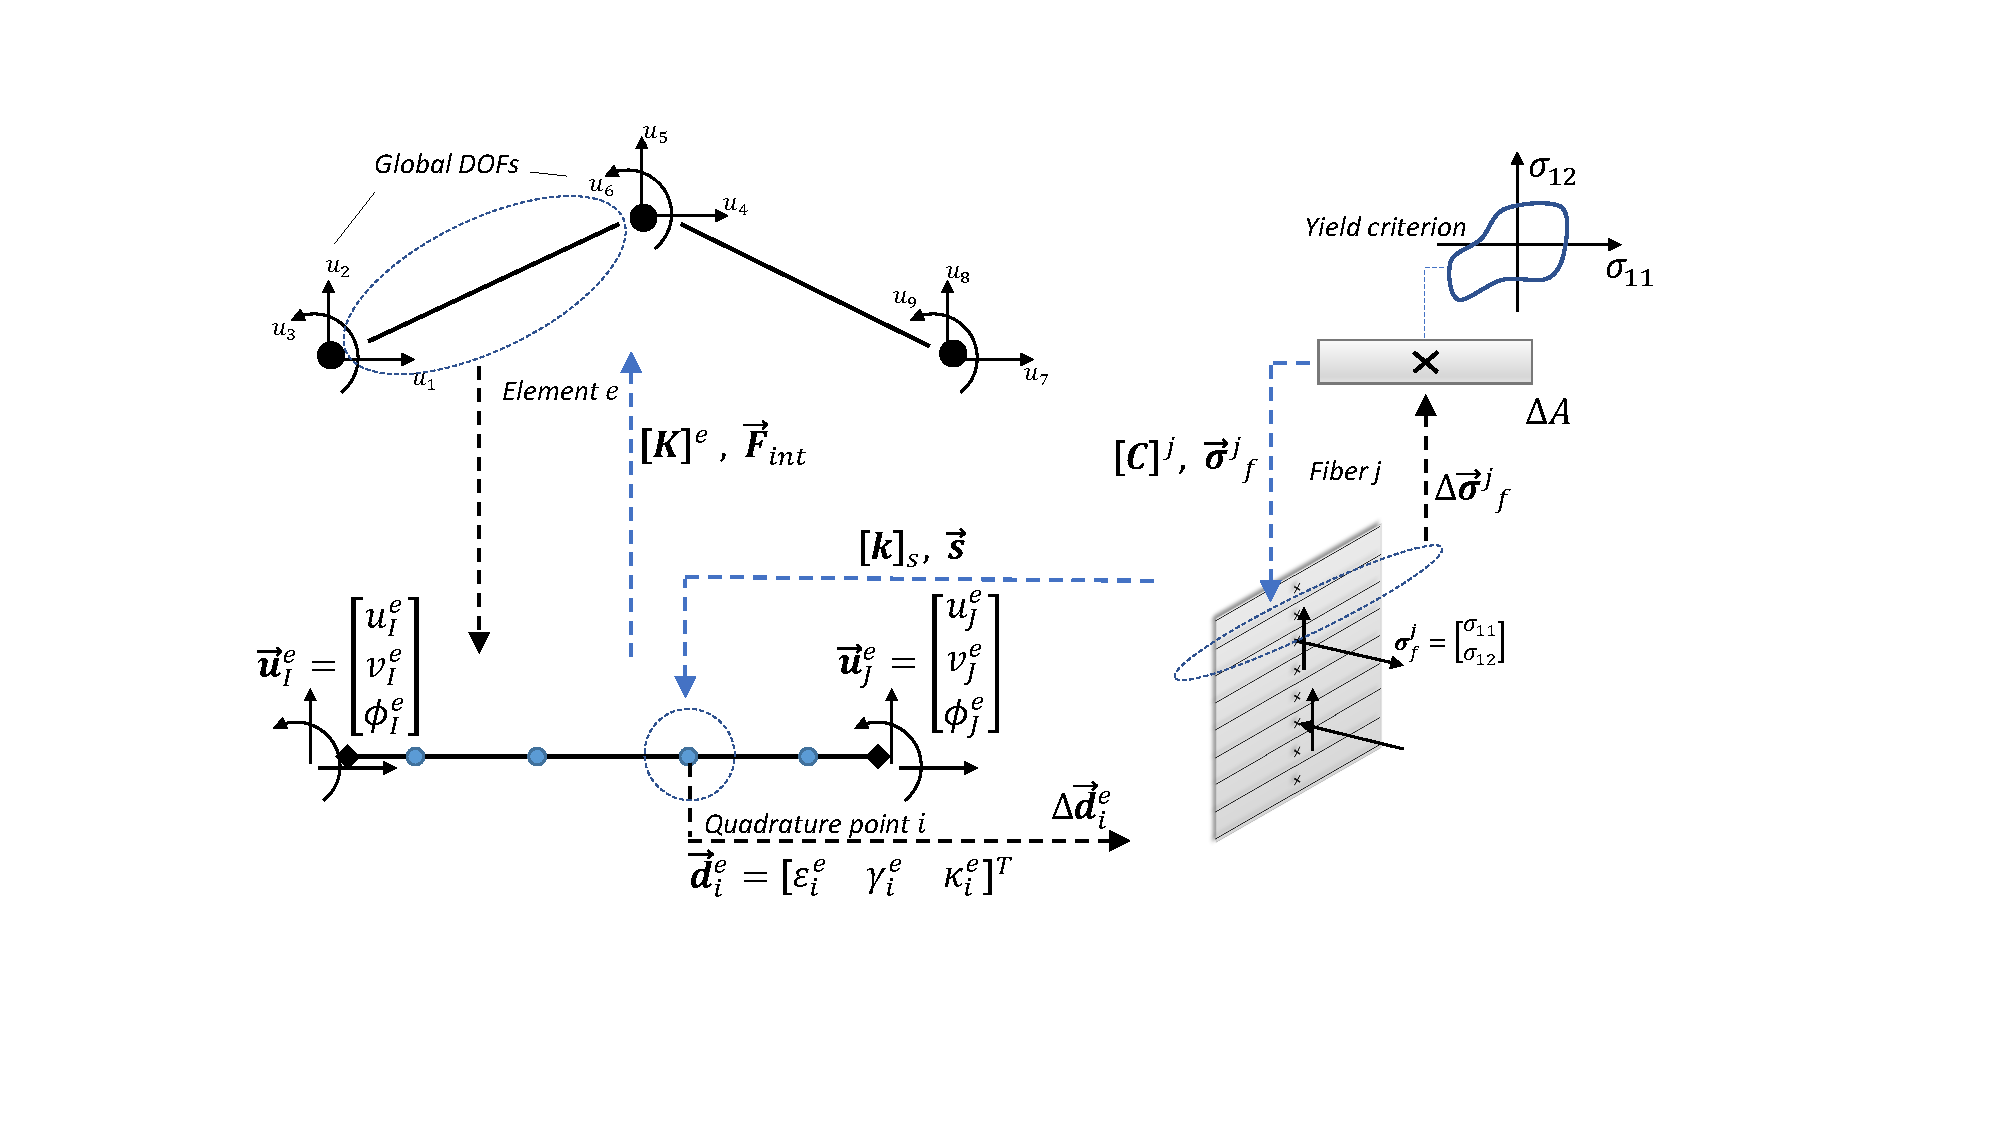
\includegraphics[scale=0.6]{FIG4_PROCESS}
	\caption{Solution process stages. Quantities $\bmat{K}^e$ and
		$\bvec{F}_{int}$ stand for stiffness matrix and internal nodal force 
		vector
		for element $e$ respectively.}
	\label{fig:FIG4_PROCESS}
\end{figure}

The generalized section stiffness,
$\nabla^2_{\mathbf{y}_i\mathbf{y}_i}\mathcal{L}$, is given by the second
derivatives of the Lagrangian with respect to strain vector
$\bvec{y}_i=\begin{bmatrix}
	\bvec{q}_i^T & \phi_i
\end{bmatrix}^T$:  % HERE
\begin{gather}
	\nabla^2_{\mathbf{y}_i\mathbf{y}_i}\mathcal{L} =
	\nabla^2_{\mathbf{y}_i\mathbf{y}_i}U
	+ \nabla_{\mathbf{y}_i}([\nabla_{\mathbf{y}_i}\bvec{h}_g]\bvec{\lambda})
	\label{eq:equivS}
\end{gather}

\noindent where:
\begin{gather}
	\nabla^2_{\mathbf{y}_i\mathbf{y}_i}U = w_i\begin{bmatrix}
		\bmat{k}_{sec}^{(i)} & \bmat{0}\\
		\bmat{0} & 0
	\end{bmatrix}\nonumber
\end{gather}

\noindent For the explicit expression of the second term in the right-hand side
of Eq. (\ref{eq:equivS}), see Appendix \ref{appendix:B}. It
generally includes parameters associated with section rotations and Lagrange
multipliers, and is greatly simplified if small displacement assumptions
are used.



%%%%%%%%%%%%%%%%%%%%% CHAPTER 2 - SECTION 4 %%%%%%%%%%%%%%%%%%%%%%%%%%%%%%
\section{Numerical Examples}\label{section:CH2-S5}
%%%%%%%%%%%%%%%%%%%%%%%%%%%%%%%%%%%%%%%%%%%%%%%%%%%%%%%%%%%%%%%%%%%%%%%%%%

In this section we present the capabilities and efficiency of the proposed
element in a number of well-known benchmark examples. In cases where analytical
solutions are available, they are included in the comparisons. Our results are
compared against the ones achieved i) with the structural \acrshort{fem} 
software
OpenSees\cite{OpenSees}, using its flexibility-based beam element
\cite{Neuenhofer,Neuenhofer2} with five quadrature points and fiber section
integration, and ii) with the \acrshort{fem} software Abaqus\cite{Abaqus}, using
plane-stress modeling for the frame members. For the
elastic analyses, reduced integration linear quadrilateral elements (CPS4R) were
used in Abaqus to avoid shear-locking, while for the elastoplastic
simulations, reduced integration quadratic quadrilaterals (CPS8R) elements
were used instead. For all cases the Gauss-Legendre
quadrature rule is used for approximating the integrals in Eqs.
(\ref{eq:tpe2}), (\ref{eq:cintform}). For the elastoplastic analyses, we assume
a linear isotropic hardening law and the elastoplastic modulus is given
as a percentage $r$ of the elastic modulus $E$. Moreover, we assume a
rigid rectangular cross-section shape for all cases, with shear coefficient
$k_s=0.870$\cite{Cowper}. For all examples, the SI units corresponding to
material and geometric properties are Pa and $m$, while for the load units
Newton(N) is used. The convergence termination criterion for the iterative
procedure was $10^{-7}$ for all cases. Shear deformation is
allowed to occur in all analyses unless stated otherwise.


\subsection{Cantilever with Tip Load}\label{CANTIPROB}

In this first example we demonstrate the element performance with fully 
nonlinear assumptions against available analytical solutions, 
as well as its locking-free behavior when small displacement assumptions
hold.

\subsubsection{Nonlinear analyses}
Both elastic and inelastic geometrically nonlinear cases are
considered. One
element and six integration points are used, with the beam assumed to be
inextensible, and the results are presented in Fig. 
\ref{fig:FIG5_cantielastic}. 
The elastic
case assumed $EI=10$, $L=1$ and shear-rigid response for comparison purposes 
with available exact equilibrium paths\cite{bisshopp}, while the inelastic
case allows for shear effects to take place with $GA_s=500$. In order to
maintain consistency with the attributes $EI=10$ and $L=1$, we used $E=200\times
10^9$ for Young's modulus and prescribed the height of the cross-section to be
$h=0.02$, which is now required in order to carry out the cross-sectional
stress-update.
For the material nonlinearity example, the yield stress is 
$\sigma_y=180\times10^7$ with a tangent-to-elastic modulus
ratio $r=3\%$ and results are compared against Abaqus and OpenSees. 
As can be seen in
Fig. \ref{fig:FIG5_cantielastic}, in both cases remarkable accuracy is 
achieved
with just one element. Slight differences between the Abaqus quadrilateral 
model and
the beam models are observed when extensive plastification takes place. In 
Table \ref{table:table1} we also provide distinct comparisons with exact
values for the elastic case. It is clear
that when the normalized load is equal to 1, displacements remain small, and
thus, only $n=4$ quadrature points suffice to achieve small absolute error. At
the maximum load level, however, $n=6$ quadrature points 
were required for highly accurate results. 
For the shear-rigid case exact solutions are computed from numerical evaluation 
of the
elliptic integrals that describe the problem. The reader can also consult Table
1 in \cite{Mattiasson} for a wide range of values reported. Additional results
pertaining to the elastic shear-flexible case are also reported in Table
\ref{table:table1}. For this case, we used again $GA_s=500$, $EI=10$, $L=1$ and 
compared against available 
analytical solutions from\cite{Batista2}, where the normalized load
level therein is held constant and equal to 1. The values corresponding to the
maximum normalized load equal to 10 are also reported. Although exact solutions
are not available for this load level to compare against, we can see that the 
relative
change in the transverse and axial displacement with respect to the shear-rigid
case is consistent and about $5.30\%$ and $5.40\%$,
respectively.

\begin{figure*}[t]
	\centering
	\subfloat[Elastic
	analysis]{{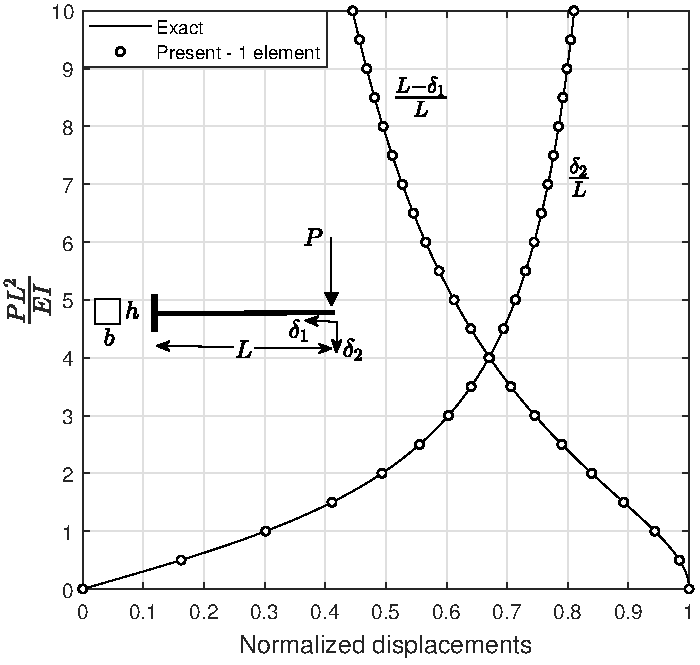
\includegraphics[width=6.5cm]{FIG5_cantiElastic_Review.pdf}}}%
	\qquad
	\subfloat[Inelastic
	analysis]{{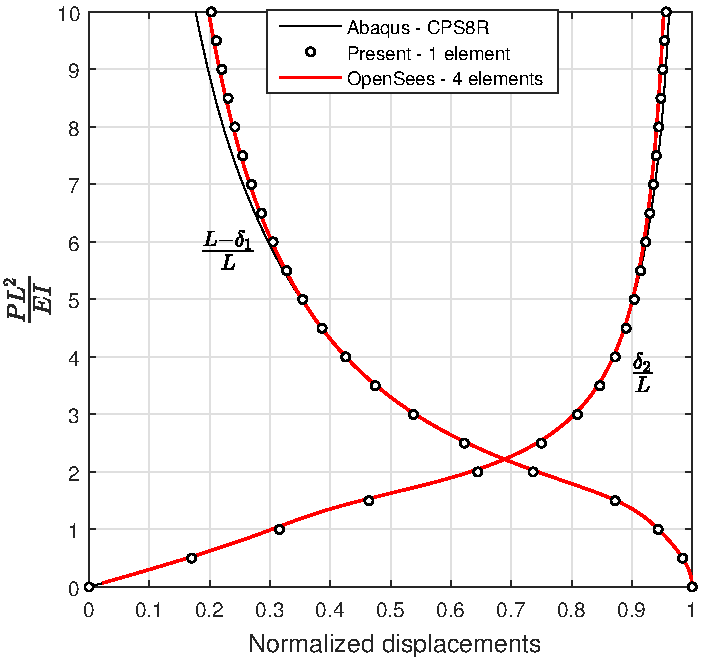
\includegraphics[width=6.5cm]{FIG5_cantiPlastic_Review.pdf}}}%
	\caption{Geometrically nonlinear analyses of cantilever.}%
	\label{fig:FIG5_cantielastic}%
\end{figure*}



\begin{figure}[t]
	\centering
	\hspace*{-0.47cm}\subfloat[Elastic.]{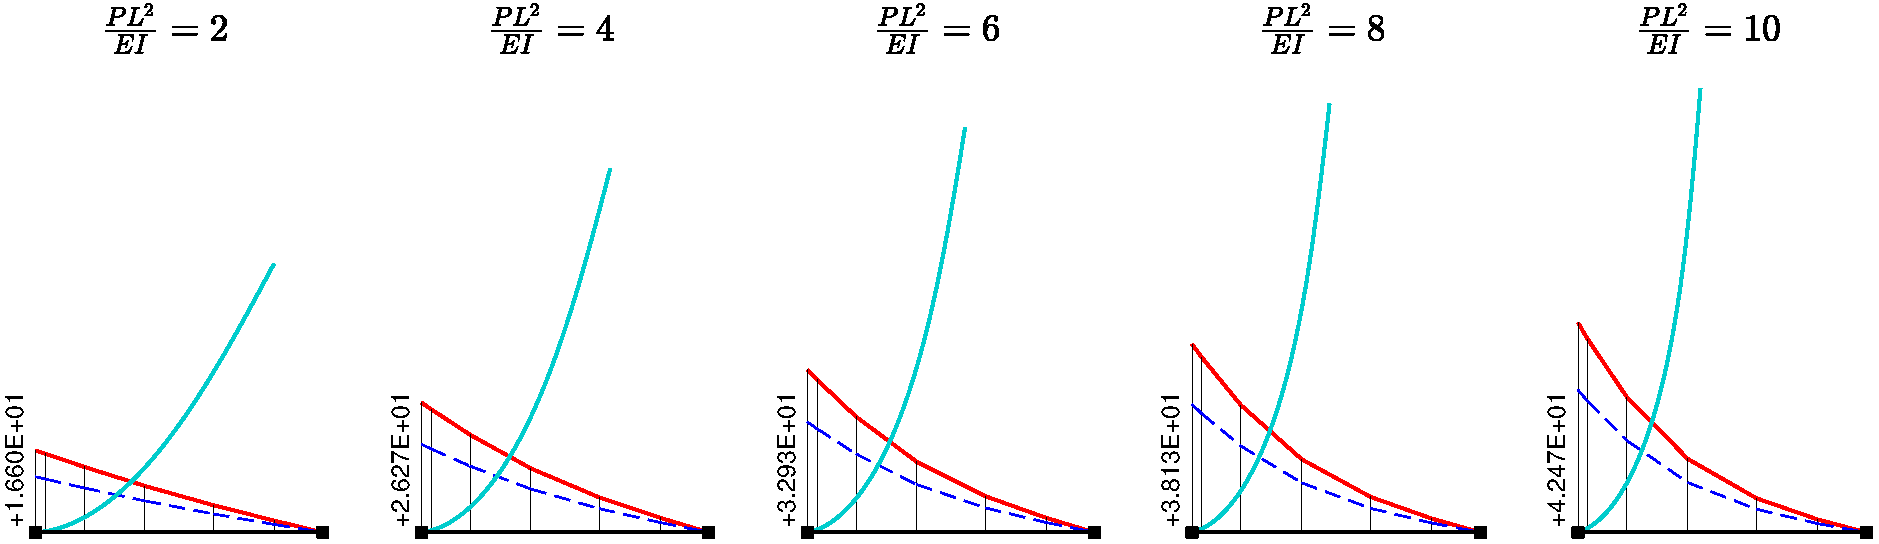
\includegraphics[scale=0.45]{FIG6_ElasticMQN.pdf}\label{fig:elasticMQN}}\\
	\hspace*{-0.47cm}\subfloat[Inelastic.]{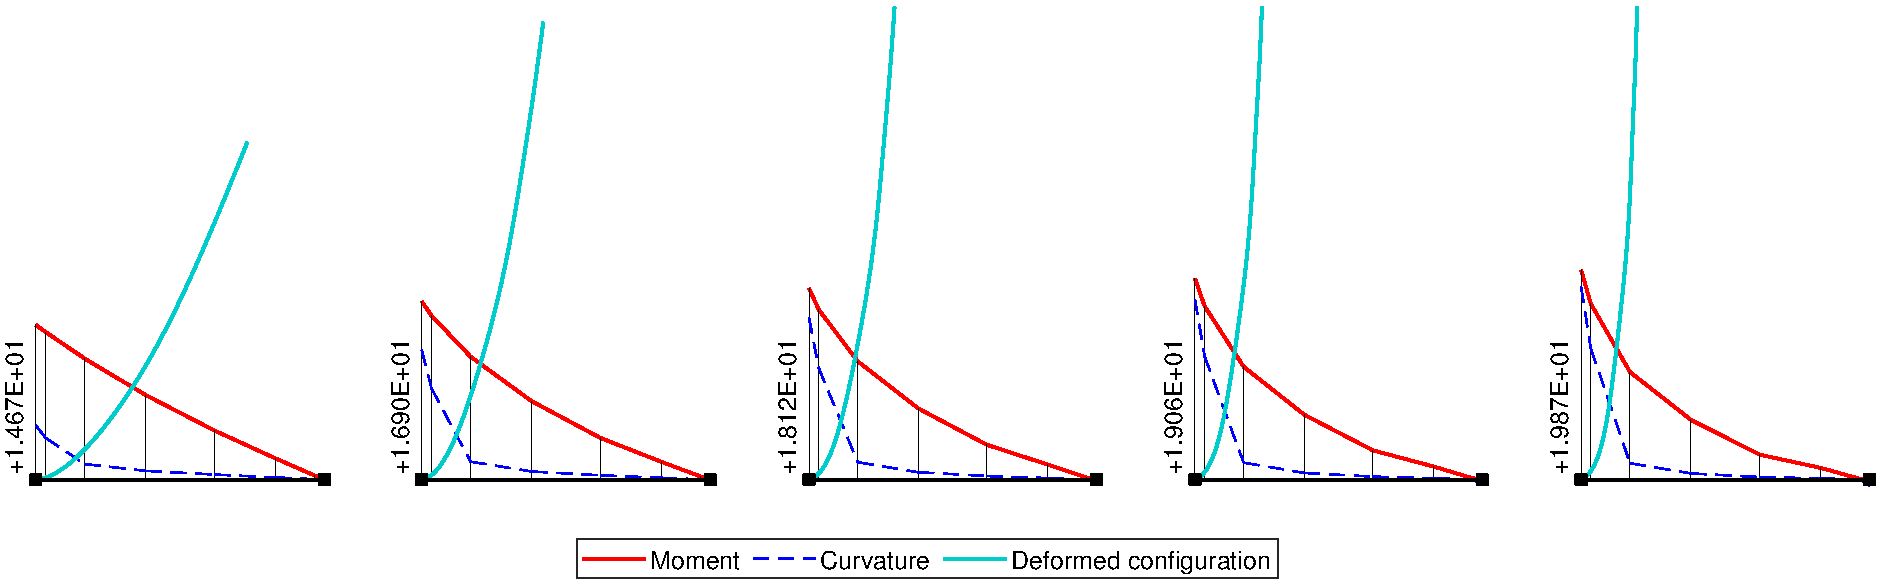
\includegraphics[scale=0.45]{FIG6_PlasticMQN.pdf}\label{fig:plasticMQN}}
	\caption{Moment and curvature distributions for the nonlinear 
		analyses of the cantilever.}
	\label{fig:FIG6_MQN}
\end{figure}

\begin{table*}[b]\centering
	\caption{Comparison of tip normalized displacements for different load 
	levels
		for elastic response.}
	\noindent\makebox[\textwidth]{
		\begin{tabular}{@ {}ccccccccc@ {}}\toprule[2pt]
			& & & \multicolumn{3}{c}{Shear Rigid}  & 
			\multicolumn{3}{c}{Shear Flexible}\\
			\cmidrule(r{.15em}l{.10em}){4-6} \cmidrule(r{0.15em}l){7-9}
			& $\frac{PL^2}{EI}$& $n$ & Exact & Present & Error & Exact & 
			Present & Error\\
			\midrule[0.9pt]
			\multirow{2}*{$\displaystyle\frac{\delta_2}{L}$}&$1$ & 4 & 
			0.3017207 & 0.3017206 & 1.12E-07 & 0.3178138 & 0.3178137 & 
			1.64E-07\\
			& $10$ & 6 & 0.8106090 & 0.8106113 & 2.32E-06 & - & 0.8536137 & - 
			\\
			\midrule%\addlinespace[3pt]
			\multirow{2}*{$\displaystyle\frac{L-\delta_1}{L}$}& 1 & 4 & 
			0.9435668 &
			0.9435666 & 1.82E-07 & 0.9386844 & 0.9386842 & 1.75E-07 \\
			& $10$ & 6 & 0.4450044 & 0.4450017 & 2.62E-06 & - & 0.4208910 & -\\
			\bottomrule[1.5pt]
		\end{tabular}
		
	}
	\label{table:table1}
\end{table*}

In Fig. \ref{fig:FIG6_MQN} we see how the moment and curvature
distributions change based on the beam deformations for both cases of Fig.
\ref{fig:FIG5_cantielastic}, captured at distinct
load levels. The moment values at the left fixed end are also reported on
the graphs. The observed nonlinear distributions for the elastic case are due 
to the
deformed shape of the beam being drastically different from its initial
configuration. As seen, an important feature of the formulation is its ability 
to capture curvature localization when plastic hinges are also formed. In 
displacement-based conventional beam elements, a fine mesh is in constrast 
required in the areas where plastification is expected.



\clearpage

\subsubsection{Shear-locking}
Shear locking may occur in shear deformable elements undergoing bending.
Due to inconsistent interpolation of fields that are naturally related, spurious
shear stresses develop and the element response appears to be stiffer,
particularly as the beam slenderness is increased. Appropriate numerical
treatments include using field consistent higher order elements or applying
reduced numerical integration \cite{Reddy,Prathap,ZienShear}. Here, we perform
small displacement elastic analyses for various length-to-thickness
ratios. The tip displacement ratios of $\delta_T/\delta_B$ and $\delta/\delta_B$
are then plotted against the length to thickness ratio $L/h$, where $\delta_B$
and $\delta_T$ denote the Bernoulli and Timoshenko displacements respectively.
Only one element is used with two integration points. The section dimensions
are kept fixed, while the length $L$ of the beam varies. Results, along
with used data are shown in Fig. \ref{fig:FIG7_lock}, where it can be seen 
that the
proposed element exhibits locking-free behavior.

\begin{figure}[t]
	\centering
	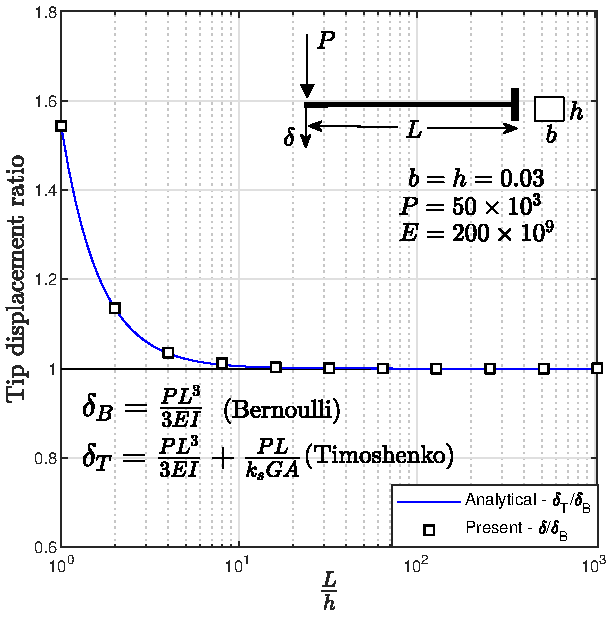
\includegraphics[scale=0.9]{FIG7_locking.pdf}
	\caption{Influence of $L/h$ on the tip deflection and comparison with
		analytical solution.}
	\label{fig:FIG7_lock}
\end{figure}


\subsection{Lee's Frame}
Lee's frame is a well-known benchmark for geometrically nonlinear capabilities
of beam-column element formulations.  It was first analyzed by Seng-Lip Lee
et.al. in
\cite{Lee} where the exact solution to the problem was also provided. We
first consider here the classic case, where the frame is pinned on both 
supports.
An investigation on the effect of shear flexibility to the elastic response
is also carried out by varying the length-to-thickness ratio, while maintaining
large-displacement assumptions. It is demonstrated that for ratios smaller than
five, the equilibrium path ceases to be similar to the shear-rigid case. Lastly,
we investigate the response of the same frame when both supports are fixed. This
again leads to a drastically different response, with abrupt changes in the
equilibrium path.  In all cases, the centerline is assumed inextensible.

\subsubsection{Frame with pinned supports}\label{leespinned}

An elastic, geometrically nonlinear analysis is first performed.
The minimum number of elements that can be used for this specific example is 
three
and a 4-point quadrature is applied for each element, whereas twelve flexibility
elements are required in OpenSees to achieve comparable accuracy.
For the elastoplastic analysis, again three elements are used in our
simulation with eight integration points,
whereas fourteen flexibility elements are now required in OpenSees for 
comparable
accuracy. The yield stress is $\sigma_y=1.3\times 10^{9}$ and the
tangent-to-elastic modulus \ratio is $r=3.00\%$. In the elastic
analysis, the
frame members are also considered shear-rigid, in order to remain consistent
to the initial assumptions in the original investigation\cite{Lee}.
Results are shown in Fig. \ref{fig:FIG8_LeesPinned}, with the colored
markers corresponding to the deformed profiles of the same color shown in
Fig. \ref{fig:FIG9_LeesPinnedProfiles}.

\begin{figure*}[t]
	\centering
	\subfloat[Elastic 
	analysis]{{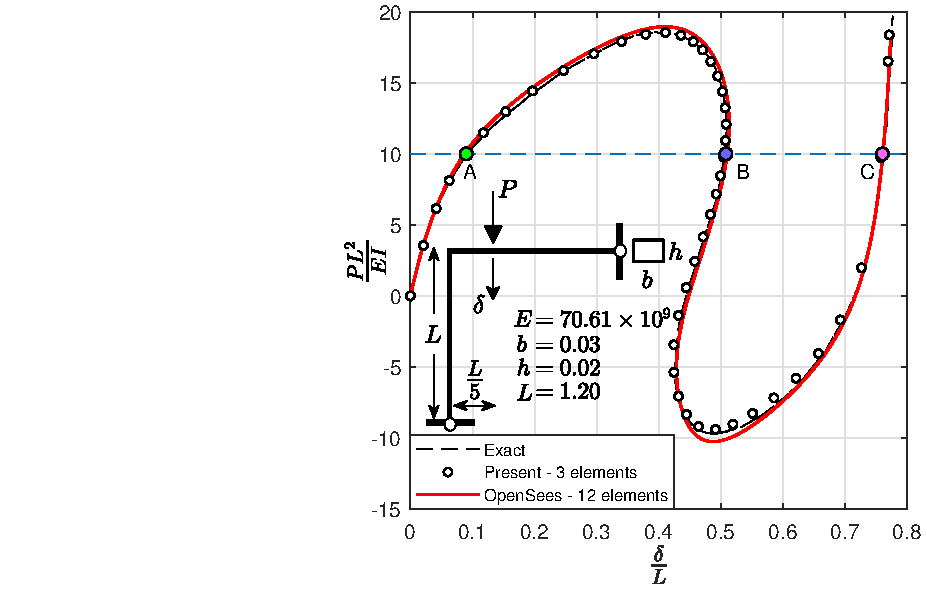
\includegraphics[width=7.cm]{FIG8_LeesElastic.pdf}}}%
	\qquad
	\subfloat[Inelastic 
	analysis]{{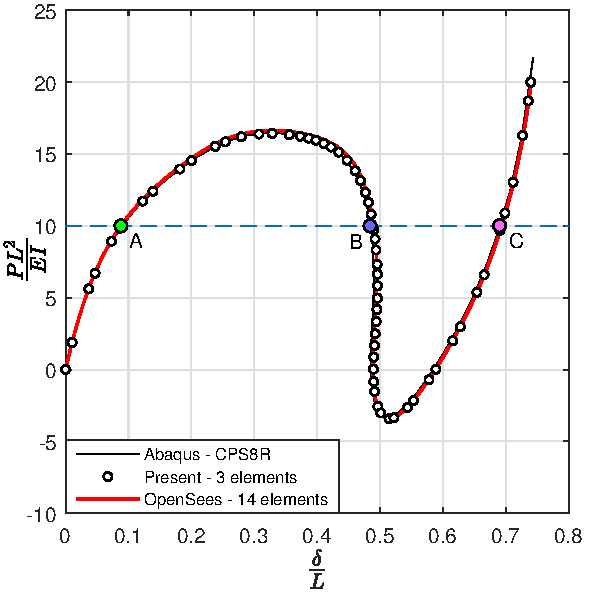
\includegraphics[width=7.cm]{FIG8_LeesPlastic.pdf}}}%
	\caption{Geometrically nonlinear analyses of Lee's frame with pinned
		supports.}%
	\label{fig:FIG8_LeesPinned}%
\end{figure*}

\begin{figure*}[b]
	\centering
	\subfloat[Elastic 
	profiles]{{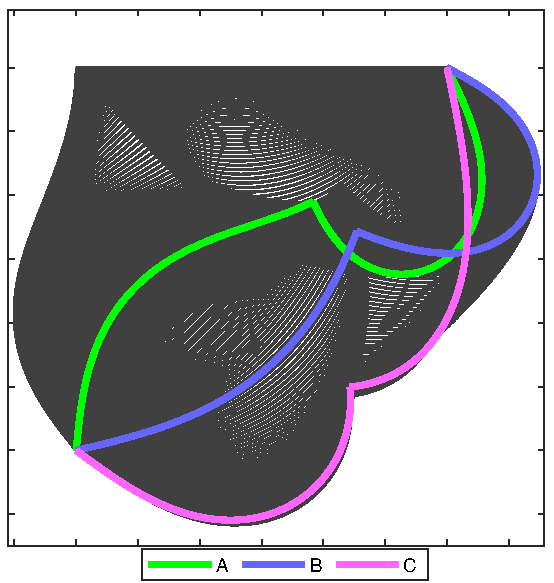
\includegraphics[width=6.5cm]{FIG9_ElasticProfiles.pdf} }}%
	\qquad
	\subfloat[Inelastic 
	profiles]{{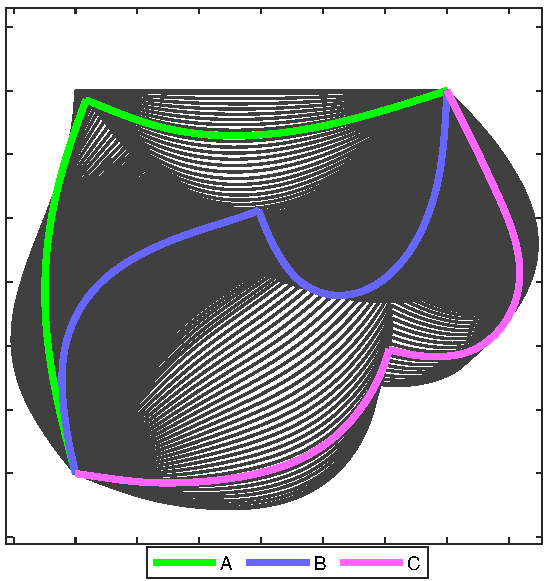
\includegraphics[width=6.5cm]{FIG9_PlasticProfiles.pdf} }}%
	\caption{Deformation profiles for Lee's frame with pinned supports.}%
	\label{fig:FIG9_LeesPinnedProfiles}%
\end{figure*}
\clearpage
In Fig. \ref{fig:FIG10_shearEffectLees}, results related to shear flexibility
effects on the frame's response are shown.  As previously mentioned, in 
\cite{Lee}
the members are assumed to be shear rigid, effectively adhering to the Bernoulli
assumptions. In this example, we relax this assumption and examine how the
slenderness decrease affects the structural response. As seen in the figure,
four different length-to-thickness ratios are examined and the equilibrium
path gradually deviates from the shear-rigid case. For ratio $L/h=4$, the
equilibrium path is drastically different and the structure, after entering the
snap-back region, follows a rather complex equilibrium branch. Note that around
$\delta/L=0.5$, the structure exits its current branch and continues on a 
similar
path as in the previous cases.

\begin{figure*}[t]
	\centering
	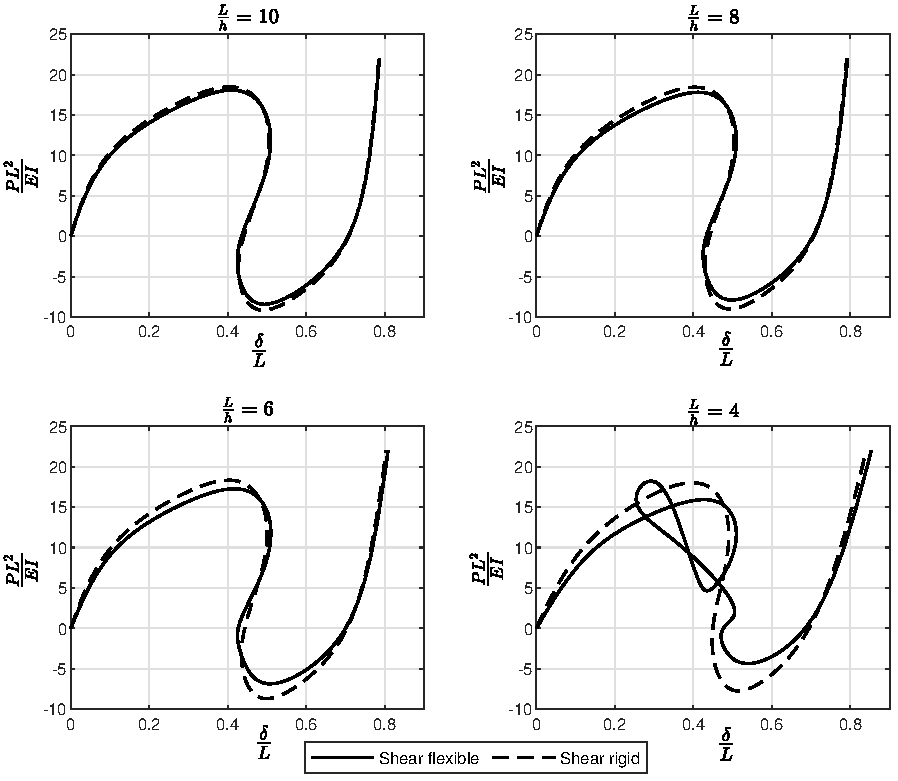
\includegraphics[scale=1]{FIG10_ElasticLHcomp.pdf}
	\caption{Effect of shear flexibility on Lee's frame response. }
	\label{fig:FIG10_shearEffectLees}
\end{figure*}

\subsubsection{Frame with fixed supports}
This variation of the benchmark problem results in a response that exhibits
a dramatic snap-back, with abrupt changes in the stiffness sign along the
equilibrium path for the nonlinear elastic problem.
Seven integration points are used here per element and, again, one element
per member, to achieve the same accuracy as with
the Abaqus plane stress model, which terminated prematurely. 
In contrast, twenty
elements are necessary in OpenSees for comparable results. The geometric
and material properties are the same as in Sec. (\ref{leespinned}) (see Fig.
\ref{fig:FIG8_LeesPinned}). For the inelastic analysis, five integration
points are sufficient, since the response is now fairly smooth overall,
in comparison to the elastic case. All members
are shear flexible in these examples, however the contribution of shear
deformation to the overall responses is negligible for both elastic and
inelastic cases.
The response and deformation profiles for both analyses are shown in Figs.
(\ref{fig:FIG11_LeesFixed}),(\ref{fig:FIG12_LeesFixedProfiles}) respectively.

\begin{figure*}[h]
	\centering
	%\subfloat[Elastic
	%profiles]{{\includegraphics[width=5.6cm]{FixedElasticProfiles_Review.pdf} 
			%}}%
	\subfloat[Elastic
	profiles]{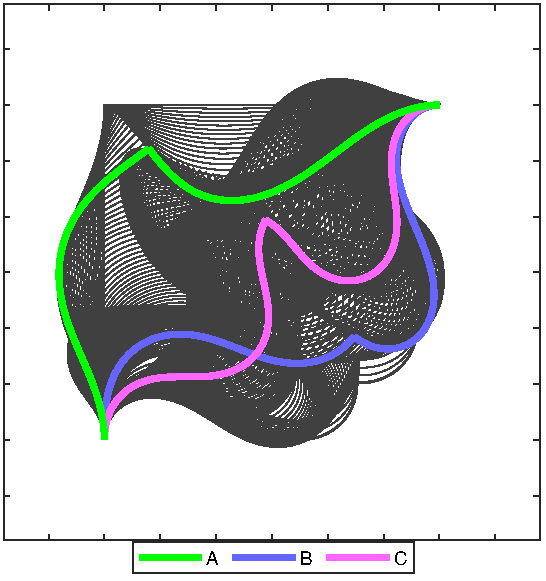
\includegraphics[width=6.5cm]{FIG12_FixedElasticProfiles_Review.pdf}}%
	\qquad
	\subfloat[Inelastic 
	profiles]{{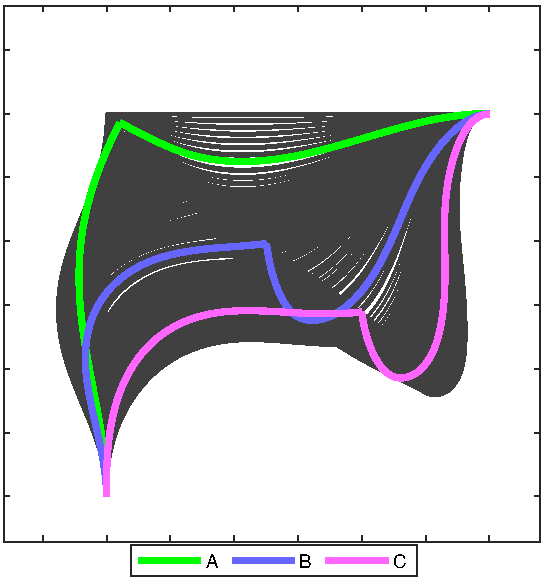
\includegraphics[width=6.5cm]{FIG12_FixedPlasticProfiles.pdf} 
	}}%
	\caption{Deformation profiles for Lee's frame with fixed supports.}%
	\label{fig:FIG12_LeesFixedProfiles}%
\end{figure*}

\clearpage
\begin{figure*}[t]
	\centering
	%\subfloat[Elastic
	%analysis]{{\includegraphics[width=8.2cm]{LeesFixedElastic_Review.pdf}}}%
	\subfloat[Elastic
	analysis]{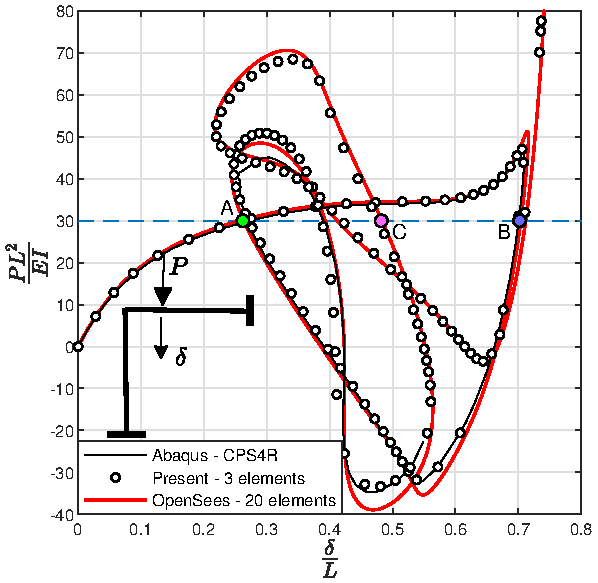
\includegraphics[width=7.cm]{FIG11_LeesFixedElastic_Review.pdf}}%
	\qquad
	\subfloat[Inelastic 
	analysis]{{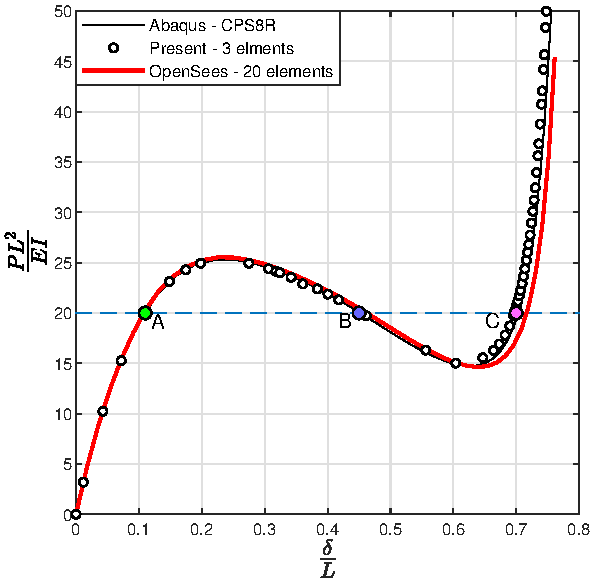
\includegraphics[width=7.cm]{FIG11_LeesFixedPlastic.pdf}}}%
	\caption{Geometrically nonlinear analyses of Lee's frame with fixed
		supports.}%
	\label{fig:FIG11_LeesFixed}%
\end{figure*}

\subsection{Two-Storey Frame}

In this example a two-story frame with one bay is analyzed, first studied
regarding its plastic limit load in \cite{horne}. It was also later used as a
benchmark example by Santos \cite{Santos1}, for the performance of a nonlinear
beam finite element based on complementary energy principles. The example
is slightly modified here, however the rectangular cross-section
dimensions of the structural members and their length $L$ have been
chosen so their the slenderness remains in accordance with
\cite{Santos1}. The yield stress is $\sigma_y=0.9\times 10^6$, and the
tangent-to-elastic modulus ratio is $r=3\%$. The full frame
characteristics and discretization are shown in Fig. 
\ref{fig:FIG13_santosStruct}.

\begin{figure}[t]
	\centering
	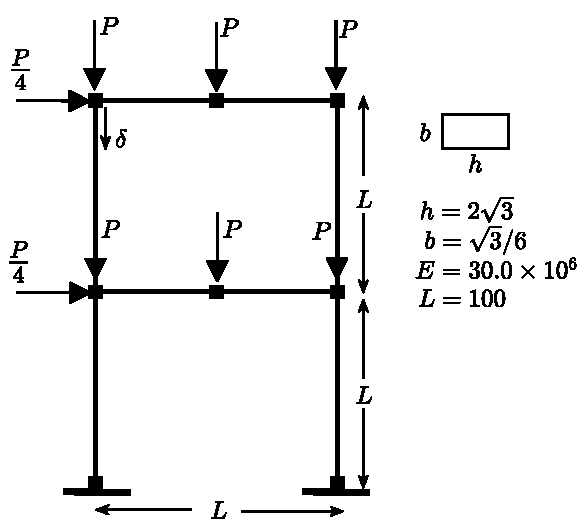
\includegraphics[width=0.7\textwidth]{FIG13_struct.pdf}
	\caption{Two-storey portal frame discretization.}
	\label{fig:FIG13_santosStruct}
\end{figure}

The minimum number of hybrid elements for this example is eight and the number
of integration points per element for the elastic and plastic analyses are
seven and ten, respectively. For the OpenSees analyses, 36 and 48 elements
were used in total for the elastic and inelastic analyses. In both cases,
however, the OpenSees analyses stopped prematurely. Results are
demonstrated in Fig. \ref{fig:FIG14_SantosAn}, showing excellent agreement 
with
Abaqus results, while the relevant deformation profiles are
provided in Fig. \ref{fig:FIG15_SantosProfiles}.

\begin{figure*}[b]
	\centering
	\subfloat[Elastic 
	analysis]{{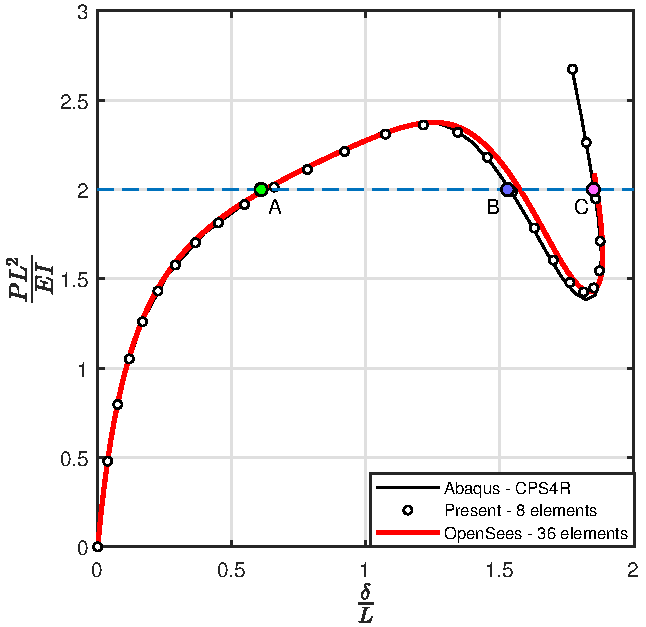
\includegraphics[width=7.cm]{FIG14_SantosElasticPaperFig.pdf} }}%
	\qquad
	\subfloat[Inelastic 
	anaysis]{{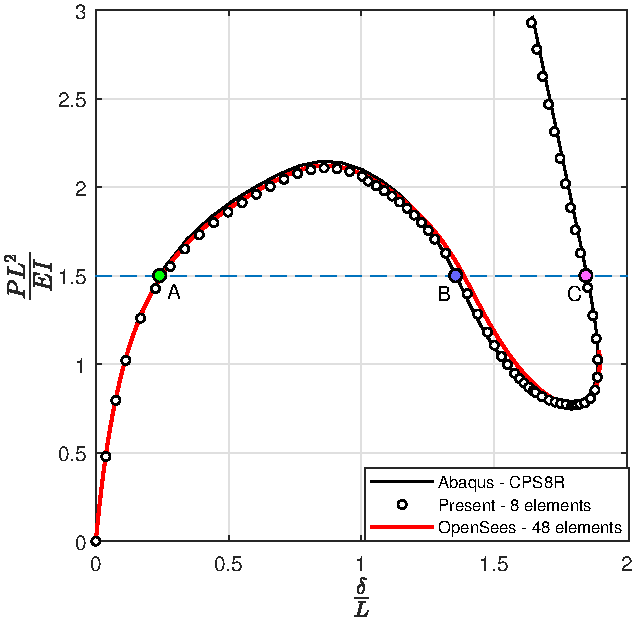
\includegraphics[width=7.cm]{FIG14_SantosPlasticPaperFig.pdf} }}%
	\caption{Geometrically nonlinear analyses of the two-storey frame.}%
	\label{fig:FIG14_SantosAn}%
\end{figure*}

\clearpage
\begin{figure*}
	\centering
	\subfloat[Elastic 
	profiles]{{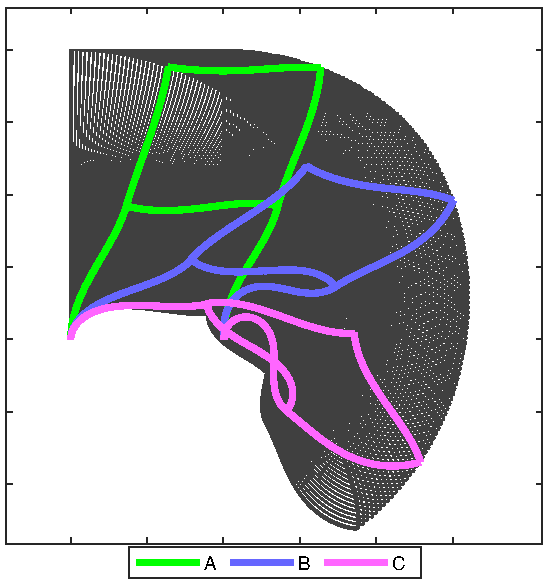
\includegraphics[width=6.5cm]{FIG15_SantosElasticProfiles.pdf} 
	}}%
	\qquad
	\subfloat[Inelastic 
	profiles]{{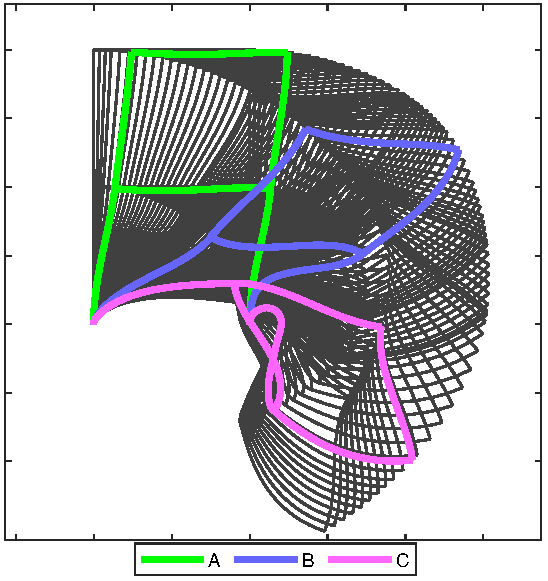
\includegraphics[width=6.5cm]{FIG15_SantosPlasticProfiles.pdf} 
	}}%
	\caption{Deformation profiles for two-storey frame.}%
	\label{fig:FIG15_SantosProfiles}%
\end{figure*}


\section{Summary}
A novel geometrically exact hybrid beam element formulation is presented in 
this work,
conceptually and numerically developed using nonlinear programming principles,
instead of the traditionally used FEM techniques. Structural analysis
is accordingly seen as a nonlinear program, where the total potential energy 
functional is
treated as the objective function of the problem, constrained in the space of
feasible kinematic configurations of the structure. Field integrals in the
objective function and kinematic constraints are functions approximated by an 
appropriate quadrature rule, and
kinematics of large displacements and rotations are modeled using the exact
strain-displacement relations of Reissner's beam theory. These kinematic 
equations serve as
constraints of the nonlinear program and are appended to the objective
function by means of Lagrange multipliers. With this formulation, the
involved shear and axial strain-related fields do not need to be
interpolated, but are rather collocated 
at certain quadrature points
inside the element, as defined by the numerical integration method. The only
interpolated field is curvature, whereas displacement unknowns eventually emerge
only at element edges. A Newton-based numerical approach to the Lagrangian of
the problem is presented, based on the second-order approximation of the 
necessary
optimality conditions, and it is also appropriately connected to
standard \acrshort{fem}
assemblage techniques. Hence, using the block elimination technique, 
\acrshort{fem} assembly 
routines can be 
directly reused, while the global stiffness is assembled from the inversion of 
local
flexibility operators. This is computationally
efficient because these matrices are processed independently and their 
dimension is upper bounded, with the number of quadrature points per element
ranging from 5 to 10. The presented approach is also capable to capturing 
flexural strain localization due to plastification even when geometric 
nonlinearities are present. The efficiency of the suggested formulation is 
demonstrated through several benchmark examples and is shown to be
capable to accurately capture highly nonlinear structural behaviors with just 
one
element per member in all cases, accounting for shear flexibility and 
locking-free capabilities, while also very favorably comparing against 
well-established 
beam-column and quadrilateral finite element methodologies.

%%%%%%%%%%%%%%%%
% Chapter 3
%%%%%%%%%%%%%%%%

\chapter{Multiaxial Material Constitutive Model for Fiber Sections}

%%%%%%%%%%%%%%%%%%%%  SECTION 1 %%%%%%%%%%%%%%%%%%%%%%%%%%%%%%%%
\section{Introduction}\label{section:CH3-S1}
%%%%%%%%%%%%%%%%%%%%%%%%%%%%%%%%%%%%%%%%%%%%%%%%%%%%%%%%%%%%%%%%

In this chapter we introduce an algorithm for shear-axial-flexure interaction 
suited for fibre beam elements of any kind (displacement-based or otherwise). 
The coupling is taken into account by considering a multiaxial constitutive law 
at the level of cross-section fibers. Thus, stress resultant interaction as 
well as the consistent tangent stiffness of a cross-section are derived during 
the state determination phase. Integration of the elastoplasic rate equations 
on each fiber is carried out using the fully backward (implicit) Euler method, 
which as is known, results in the so-called closest point projection algorithm. 
In addition, the constrained stress state of a fiber is exploited in order to 
devise a return-mapping scheme that avoids incorporating stress components that 
are not energetically active. The appropriate mapping on the constrained space 
is inspirited by the work of Simo\cite{Simo1986} and appropriately adapted for 
fibre 
discretized elements. This leads to a stress update algorithm that is 
significantly faster while also requiring less memory requirements for storage 
of non-active tensor components, compared to formulations that utilize a 
general three 
dimensional 
algorithm\cite{Papachristidis2010,Saritas2009,Ceresa2009,Gregori2007,Kagermanov2017}.
 In the latter case, stress update is a nested 
procedure within an outer Newton iteration which is necessitated in order to 
enforce the constraint for the transverse stress components, $\sigma_{22}=\ 
\sigma_{33}=0$. This is because during the trial phase of a plastic step, the 
transverse components become non-zero. Furthermore, a static condensation of 
the three-dimensional consistent tangent is required to enforce both the local 
Newton scheme and to derive the consistent tangent modulus pertaining to the 
fiber stress state. The algorithm introduced in this chapter bypasses the need 
for additional outer iterations, thereby resulting in a much faster stress 
update procedure.

For the exposition we adopted the $J_2$ consitutive model which is based on the 
von Mises yield criterion, which is suited for modelling the elastoplastic 
response of metals. Linear kinematic and general isotropic hardening are 
incorporated in the formulation. Moreover, infinitesimal strains and a 
rate-independent associative plasticity framework are the core assumptions that 
underlie the proposed algorithm. 

This chapter is subdivided in three main 
sections: first, we briefly outline the general (rate) form of the 
three-dimensional elastoplastic equations. In the second section we present the 
rate constitutive model as it pertains to the fiber stress state and derive 
expressions for the continuous elastoplastic moduli. In the third 
section we outline the implementation details, which are based on application 
of the fully implicit Euler scheme. In addition we derive the expression for 
the consistent tangent modulus at a fiber, which is required to ensure 
quadratic rates of convergence for the global Newton method. Finally, we 
conclude this chapter with a section dedicated to the assessment of the 
proposed algorithm. Accuracy is demonstrated through iso-error maps for both 
perfect and hardening plasticity. Furthermore, we compare the performance in 
terms of total plastic step iterations required for i) the present formulation, 
ii) the general, three-dimensional, and iii) the plane stress return mapping 
algorithm developed in \cite{Simo1986}. Numerical examples pertaining to 
ultimate collapse load, cyclic loading, elastoplastic buckling and a pushover 
analysis of a steel frame are also included to highlight the capabilities of 
the Hybrid \acrshort{nlp} element equipped with the multiaxial stress-update 
algorithm proposed herein.


%%%%%%%%%%%%%%%%%%%%  SECTION 2 %%%%%%%%%%%%%%%%%%%%%%%%%%%%%%%%
\section{Three-dimensional Constitutive Model}\label{section:CH3-S2}
%%%%%%%%%%%%%%%%%%%%%%%%%%%%%%%%%%%%%%%%%%%%%%%%%%%%%%%%%%%%%%%%
Below we outline the general form of rate-independent elastoplasticity 
with combined isotropic and linear kinematic hardening. Infinitesimal strains 
and associative plasticity are assumed, while the yield criterion is 
purposefully unspecified at this state in order to maintain generality. 

Let $\bm{\sigma},\ \bm{\epsilon}$ be the second order symmetric stress and 
strain tensors. We introduce the internal hardening variables $\bm{\alpha}$ and 
$q$ which represent the second order back-stress tensor and the equivalent 
uniaxial yield stress respectively. The former is associated with kinematic 
hardening while the latter models isotropic hardening. Finally, consider the 
decomposition of the strain tensor into elastic and plastic parts as follows:
\begin{equation}
	\bm{\epsilon} = \bm{\epsilon}^{el} + \bm{\epsilon}^{pl}
	\label{eq:DECOMP_STRAIN}
\end{equation} 

Then the rate form of the constitutive equations for the assumptions mentioned 
above is the following:
\begin{subequations}
	\begin{alignat}{3}
		&\dot{\bm{\epsilon}} &&= \dot{\bm{\epsilon}}^{el} +
		\dot{\bm{\epsilon}}^{pl}\quad& \text{(Strain 
		decomposition)}\label{eq:RATE_DECOMP}\\
		&\dot{\bm{\sigma}} &&= \mathbb{C}^{el}\left[\dot{\bm{\epsilon}} -
		\dot{\bm{\epsilon}}^{pl} \right]\quad& \text{(Elastic constitutive 
		law)}\label{eq:CONSTITUTIVE_LAW}\\
		&\dot{\bm{\epsilon}}^{pl} &&= \dot{\lambda}\frac{\partial \Phi}{\partial
			\bm{\sigma}}\quad& \text{(Flow rule)}\label{eq:FLOW_RULE}\\
		&\dot{\bm{\alpha}} &&= -\dot{\lambda}H_{kin}\frac{\partial 
		\Phi}{\partial
			\bm{\alpha}}\quad& \text{(Kinematic
			hardening law)}\label{eq:BACK_STRESS}\\
		&\dot{q} &&= \frac{\partial q}{\partial
			e^{pl}}\dot{e}^{pl}\quad& \text{(Isotropic hardening law)}
		\label{eq:CURRENT_YIELD_STRESS}\\
		&\dot{e}^{pl} &&= \dot{\lambda}\quad& \text{(Equivalent plastic 
		strain)}\label{eq:EQUIV_PLASTIC_STRAIN}\\
		&\Phi(\bm{\sigma},\bm{\alpha},e^{pl}) &&= 
		\sigma_{eq}(\bm{\sigma},\bm{\alpha}) - q(e^{pl}) \leq 0\quad&
		\text{(Yield criterion)}\label{eq:YIELD_FUNC} 
	\end{alignat}
	\label{eq:THREE_D_RATE}
\end{subequations}

In the above system of differential-algebraic equations, $\lambda$ is the 
plastic
parameter, $H_{kin}$ is the kinematic hardening modulus, $\mathbb{C}^{el}$ is 
the elastic moduli, a fourth order tensor, of the material and $\sigma_{eq}$ is 
the equivalent stress, which is determined by the
yield criterion used. Furthermore, in the case of linear
isotropic hardening with modulus $H_{iso}$, the corresponding harening law (Eq. 
\ref{eq:CURRENT_YIELD_STRESS}) becomes $\dot{q} =
H_{iso}\dot{e}^{pl}$, where $e^{pl}$ is the equivalent plastic strain. Finally, 
with the inequality in Eq. (\ref{eq:YIELD_FUNC})
we define a feasible stress space such that stress points stictly satisfying the
inequality, $\Phi<0$ represent an elastic state while these points that cause 
plastic flow render $\Phi$ zero.

The so-called Karush-Kuhn-Tucker loading/unloading conditions derived from the 
underlying constrained variational problem\cite{Simo2006} can be stated as
follows:
\begin{equation}
	\Phi\leq 0,\qquad \dot{\lambda} \geq 0,\qquad \dot{\lambda}\Phi=0
	\label{eq:KKT_CONDITIONS}
\end{equation}

From these conditions we can determine the current stress state:
\begin{itemize}
	\item if $\dot{\lambda}>0$, then $\dot{\lambda}\Phi=0$ implies $\Phi=0$ 
	which 
	means 
	the state is plastic
	\item if $\Phi<0$, then $\dot{\lambda}\Phi=0$ implies $\dot{\lambda}=0$ and 
	from 
	(\ref{eq:FLOW_RULE}) we get that the state is elastic.
\end{itemize}
Since $\Phi=0$, $\dot{\lambda}>0$ when plastic loading persists, the third 
equation
in (\ref{eq:KKT_CONDITIONS}) leads to the so-called plastic consistency
condition:
\begin{equation}
	\dot{\lambda}\dot{\Phi}=0
	\label{eq:PLASTIC_CONSISTENCY_CONDITION}
\end{equation}

%%%%%%%%%%%%%%%%%%%%  SECTION 3 %%%%%%%%%%%%%%%%%%%%%%%%%%%%%%%%
\section{The \texorpdfstring{$J_2$}{text} Formulation for Fiber Stress 
State}\label{section:CH3-S3}
%%%%%%%%%%%%%%%%%%%%%%%%%%%%%%%%%%%%%%%%%%%%%%%%%%%%%%%%%%%%%%%%

%%%%%%%%%%%%%%%%%%%%  SECTION 3 - SUBSECTION 1 %%%%%%%%%%%%%%%%%%%%%%%%%%%%%%%%
\subsection{Mapping on the Constrained Stress Space}\label{section:CH3-S3SS1}

We begin by defining the admissible stress space for a planar beam fiber, 
$\mathcal{S}$:
\begin{equation*}
	\mathcal{S} = \{\bvec{\sigma}\in\mathbb{R}^6\ |\
	\sigma_{22}=\sigma_{33}=\sigma_{23}=\sigma_{13}=0\}
\end{equation*}

\noindent The von Mises yield criterion is stated as follows:
\begin{equation}
	\Phi(J_2,e^{pl}) = \sqrt{3J_2} - q(e^{pl}) \leq 0
	\label{eq:VON_MISES_FUNC}
\end{equation}
where $J_2$
is the second invariant of the deviatoric stress tensor:
\begin{equation}
	J_2 = \frac{1}{2}\bm{\sigma}^d:\bm{\sigma}^d
	\label{eq:J2}
\end{equation}
The deviatoric part of any tensor is given by $(\ )^d=(\ 
)-\frac{1}{3}\bmat{I}\cdot\text{trace}[(\ )]$, with $\bmat{I}$ being the 
identity tensor and symbol ":" designates the contraction operator: 
$\bm{\sigma}^d:\bm{\sigma}^d = \sum_{i,j}\sigma_{ij}^d\sigma_{ij}^d$.

In the von Mises $J_2$ framework, the hydrostatic pressure cannot cause plastic
flow.
In other words, plastic deformation is due to the deviatoric components of the 
stress tensor and volume changes are caused only by elastic deformations. This
implies that trace[$\bm{\epsilon}^{pl}$]$=0$ which, coupled with Eq.
(\ref{eq:BACK_STRESS}), also leads to trace[$\bm{\alpha}^{pl}$]$=0$. This means 
that
the back stress tensor in Eq. (\ref{eq:BACK_STRESS}) deviatoric.

In active stress space $\mathcal{S}$ the yield function is 
$\Phi = \sqrt{\sigma_{11}^2 + 3\sigma_{12}^2}-q$ describes an ellipse, shown
in Fig. \ref{fig:FIG16_YIELDLOCUS}, with
semi-major and semi-minor axes $\sigma_y$, $\sqrt{3}^{}/3\sigma_y$, 
respectively.

\begin{figure}[t]
	\centering
	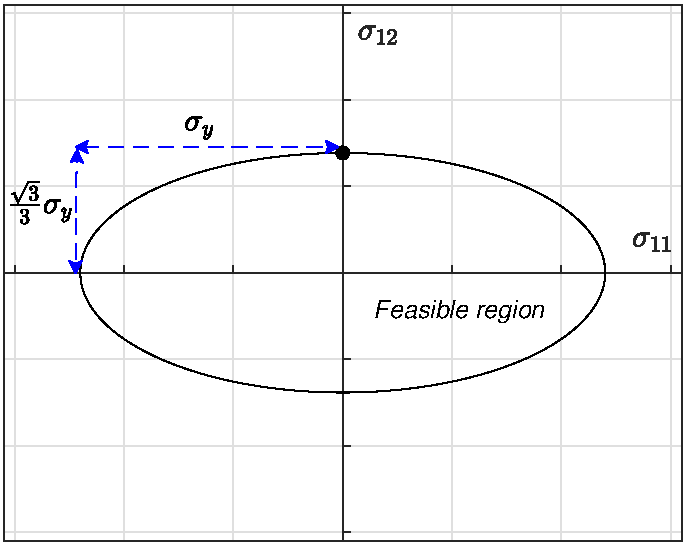
\includegraphics[scale=0.8]{FIG16_YIELDLOCUS}
	\caption{Feasible space and yield locus for the planar fiber constrained 
	$J_2$ model. At the ellipse boundary we have $\sqrt{3J_2}=q$.}
	\label{fig:FIG16_YIELDLOCUS}
\end{figure}

When kinematic
hardening is included, we introduce the effective stress tensor, 
$\bm{\zeta}$, in order to facilitate notational simplicity. Its deviatoric 
part, 
which plays central role in the three-dimensional formulation of the $J_2$ 
model is given by:
\begin{equation}
	\bm{\zeta}^d =	\bm{\sigma}^d-\bm{\alpha}^d
	\label{eq:EFFECTIVE_STRESS}
\end{equation}

We now seek a mapping from the deviatoric stress space onto the fiber stress 
space $S$ such that the inner product in the expression for $J_2$ is preserved. 
For this purpose, and in line with the vector notation for stress and strain 
tensors adopted earlier, we define the following vectors which involve only 
these tensor components that explicitly enter subsequent derivations:

\begin{gather}
	\bvec{\alpha}_f = \begin{bmatrix} \alpha_{11} \\ \alpha_{12} 
	\end{bmatrix},\quad
	\bvec{\alpha}^d_f = \begin{bmatrix} \alpha_{11}^d \\ \alpha_{12}^d 
	\end{bmatrix},\quad
	\bvec{\epsilon}^{pl}_f = \begin{bmatrix} \epsilon^{pl}_{11} \\ 
		\gamma^{pl}_{12} \end{bmatrix},\nonumber\\
	\hspace{-0.4cm}\bvec{\sigma}^d_f = \begin{bmatrix} \sigma^d_{11} \\ 
	\sigma^d_{12}
	\end{bmatrix},\quad\hspace{0.15cm}
	\bvec{\zeta}_f = \begin{bmatrix}
		\zeta_{11} \\ \zeta_{12}
	\end{bmatrix},\quad\hspace{0.15cm}
	\bvec{\zeta}_f^d = \begin{bmatrix}
		\zeta_{11}^d \\ \zeta_{12}^d
	\end{bmatrix}\nonumber
%	\label{eq:FIBER_J2_VECTORS}
\end{gather}

The subscript $f$ indicates that the vector involves only these tensor 
components pertinent to the fiber stress state. The non-zero components of 
$\bvec{\zeta}^d$ are $\zeta_{11}^d,\ \zeta_{22}^d,\ \zeta_{33}^d,\
\zeta_{12}^d,\ \zeta_{21}^d$ and thus we can establish the following mappings
between the active components of $\bvec{\zeta}^d$ and $\bvec{\zeta}_f$:
\begin{equation}
	\bvec{\zeta}^d = \bmat{Q}\bvec{\zeta}_f,\qquad \bvec{\zeta}^d_f =
	\bmat{S}\bvec{\zeta}_f
	\label{eq:MAPPING}
\end{equation}
where the mapping matrices above are given by:
\begin{equation}
	\bmat{Q} = \begin{bmatrix}
		\frac{2}{3} & -\frac{1}{3} & -\frac{1}{3} & 0 & 0 & 0 \\
		0 & 0 & 0 & 1 & 0 & 0
	\end{bmatrix}^T,\qquad \bmat{S} = \begin{bmatrix}
		\frac{2}{3} & 0\\
		0 & 1
	\end{bmatrix}
	\label{eq:MAPPING_MATRIX}
\end{equation}
where the value of $Q_{24} = 2$ because of the stress tensor symmetry.

%%%%%%%%%5

The vector representation of (\ref{eq:J2}) in terms of the effective stress is:
\begin{equation}
	J_2 = \frac{1}{2}(\bvec{\zeta}^d)^T\bmat{J}\bvec{\zeta}^d 
	\label{eq:VECTOR_J2_3D}
\end{equation}
\noindent where matrix $\bmat{J} = \text{diag}[1, 1, 1, 2,2,2]$ is introduced to
account for the symmetry of $\bm{\zeta}^d$. If the axisymmetric version of 
vectors is used, where only 4 tensor components are stored, then $\bmat{J} = 
\text{diag}[1, 1, 1, 2,]$.

We can now express $J_2$ in terms of $\bvec{\zeta}_f$:
\begin{equation}
	J_2 = \frac{1}{2}(\bvec{\zeta}^d)^T\bmat{J}\bvec{\zeta}^d = 
	\frac{1}{2}\bvec{\zeta}_f^T\bmat{Q}^T\bmat{J}\bmat{Q}\bvec{\zeta}_f =
	\frac{1}{2}\bvec{\zeta}_f^T\bmat{V}\bvec{\zeta}_f = \frac{1}{2}\Vert
	\bvec{\zeta}_f\Vert^2_{\bm{V}}
	\label{eq:J2_EQUIV}
\end{equation}
where $\bmat{V} =\text{diag}[\frac{2}{3}, 2]$ and the notation used for the 
inner product induced by matrix $\bmat{A}$ between vectors 
$\bvec{w},\ \bvec{v}$ is $(\bvec{w},\bvec{v})_{\bm{A}} =
\bvec{w}^T\bmat{A}\bvec{v}$, which leads to the notation adopted in Eq. 
(\ref{eq:J2_EQUIV}).

With these derivations at hand, system (\ref{eq:THREE_D_RATE}) can be recast in
the constrained fiber stress state as follows:
\begin{subequations}
	\begin{alignat}{3}
		&\dot{\bvec{\epsilon}}_f &&= \dot{\bvec{\epsilon}}_f^{el} +
		\dot{\bvec{\epsilon}}_f^{pl}\quad& \text{(Strain
			decomposition)}\label{eq:FIBER_RATE_DECOMP}\\
		&\dot{\bvec{\sigma}}_f &&= \bmat{C}^{el}\left[\dot{\bvec{\epsilon}}_f -
		\dot{\bvec{\epsilon}}_f^{pl} \right]\quad& \text{(Elastic constitutive
			law)}\label{eq:FIBER_CONSTITUTIVE_LAW}\\
		&\dot{\bvec{\epsilon}}_f^{pl} &&= \dot{\lambda}\bvec{n}\quad& 
		\text{(Flow
			rule)}\label{eq:FIBER_FLOW_RULE}\\
		&\dot{\bvec{\alpha}}_f &&= 
		\dot{\lambda}H_{kin}\bmat{V}^{-1}\bvec{n}\quad& \text{(Kinematic
			hardening law)}\label{eq:FIBER_BACK_STRESS}\\
		&\dot{q}_f &&= \dot{\lambda}\frac{\partial q_f}{\partial
			e_f^{pl}}\quad& \text{(Isotropic hardening law)}
		\label{eq:FIBER_CURRENT_YIELD_STRESS}\\
		&\Phi(\bvec{\zeta}_f,e^{pl}) &&=
		\sqrt{\frac{3}{2}}\Vert\bvec{\zeta}_f\Vert_{\bm{V}} - q_f(e_f^{pl}) 
		\leq 0\quad&
		\text{(Yield criterion)}\label{eq:FIBER_J2_YIELD_FUNC} 
	\end{alignat}
	\label{eq:FIBER_RATE_SYSTEM}
\end{subequations}

\noindent Vector $\bvec{n}$ is expressed as follows:
\begin{equation}
	\bvec{n} =  \frac{\partial \Phi}{\partial \bm{\sigma}_f} = 
	- \frac{\partial \Phi}{\partial \bm{\alpha}_f} =
	\sqrt{\frac{3}{2}}\frac{\bmat{V}\bvec{\zeta}_f}{\Vert\bvec{\zeta}_f\Vert_{\bm{V}}}
	\label{eq:VECTOR_n}
\end{equation}
Equations (\ref{eq:CURRENT_YIELD_STRESS}), (\ref{eq:EQUIV_PLASTIC_STRAIN})
remain the same in the current system. In addition, note that for the 
$J_2$ model, the left-hand side of eq. (\ref{eq:BACK_STRESS}) is a deviatoric 
tensor whereas in (\ref{eq:FIBER_BACK_STRESS}) it has been mapped to fiber 
stress space $\mathcal{S}$.


%%%%%%%%%%%%%%%%%%%%  SECTION 3 - SUBSECTION 2 %%%%%%%%%%%%%%%%%%%%%%%%%%%%%%%%
\subsection{Continuous Tangent Modulus}\label{section:CH3-S3SS2}

The continuous elastoplastic modulus $\bmat{C}^{ep}$ is found by enforcing the
plastic consistency condition (\ref{eq:PLASTIC_CONSISTENCY_CONDITION}) during a 
plastic step:
\begin{equation}
	\bvec{n}^T\dot{\bvec{\zeta}}_f-\dot{\lambda}\frac{\partial q_f}{\partial
		e_f^{pl}} = 0
	\label{eq:FIBER_PLASTIC_CONSISTENCY_ENF}
\end{equation}
The rate form for the effective stress is given by combining Eqs.
(\ref{eq:FIBER_CONSTITUTIVE_LAW}), (\ref{eq:FIBER_BACK_STRESS}) with
$\dot{\bvec{\zeta}}_f = \dot{\bvec{\sigma}}_f - \dot{\bvec{\alpha}}_f$:
\begin{equation}
	\dot{\bvec{\zeta}}_f = \bmat{C}^{el}\dot{\epsilon}_f -
	\dot{\lambda}\bmat{Z}\bvec{n}
	\label{eq:RATE_FORM_EFFECTIVE}
\end{equation}
\noindent where $\bmat{Z} = \bmat{C}^{el}+H_{kin}\bmat{V}^{-1}$.
Substituting (\ref{eq:RATE_FORM_EFFECTIVE}) into
(\ref{eq:FIBER_PLASTIC_CONSISTENCY_ENF}) and solving for $\dot{\lambda}$ we get:
\begin{equation}
	\dot{\lambda} =
	\frac{\bvec{n}^T\bmat{C}^{el}\dot{\bvec{\epsilon}}_f}{\bvec{n}^T\bmat{Z}\bvec{n}+
		\frac{\partial q_f}{\partial e_f^{pl}}}
	\label{eq:PLASTIC_PARAM_RATE}
\end{equation}
Finally, by making use of (\ref{eq:PLASTIC_PARAM_RATE}),
(\ref{eq:FIBER_FLOW_RULE}) and (\ref{eq:FIBER_CONSTITUTIVE_LAW}), we arrive at
the expression for the continuous elastoplastic modulus:
\begin{equation}
	\bmat{C}^{pl} =
	\bmat{C}^{el}-\frac{\bvec{m}\bvec{m}^T}{\bvec{n}^T\bmat{Z}\bvec{n}+
		\frac{\partial q_f}{\partial e_f^{pl}}}
	\label{eq:CONT_ELASTOPLASTIC_MODULUS}
\end{equation}
\noindent where $\bvec{m} = \bmat{C}^{el}\bvec{n}$.

%%%%%%%%%%%%%%%%%%%%  SECTION 4 %%%%%%%%%%%%%%%%%%%%%%%%%%%%%%%%
\section{Implicit Integration of Rate Equations}\label{section:CH3-S4}
%%%%%%%%%%%%%%%%%%%%%%%%%%%%%%%%%%%%%%%%%%%%%%%%%%%%%%%%%%%%%%%%

We employ the fully implicit backward Euler method to discretize the rate
constitutive equations in system (\ref{eq:FIBER_RATE_SYSTEM}) in the pseudotime
interval $[t_n,t_{n+1}]$. We regard the incremental/iterative process as strain
driven, in that at the start of increment $n$, the dependent state variables 
for each fiber,
$S_{f,n}=\{\bvec{\epsilon}_f,\bvec{\epsilon}_f^{pl},\bvec{\alpha}_f,e_f^{pl}\}_n$,
 
are
known and stored. We also know the increment in the centerline strain vector
$\bvec{d}$, $\Delta\bvec{d}$. The incremental strain vector for the current
fiber is then determined using eq. (\ref{eq:f2}):
\begin{equation*}
	\Delta\bvec{\epsilon}_f = \bmat{N}_s\Delta\bvec{q}
	\label{eq:INCREMENTAL_STRAINS}
\end{equation*}
Given the incremental strain vector $\Delta\bvec{\epsilon}_f$, 
we need to update the state variables for $t_{n+1}$:  $S_{f,n}\rightarrow 
S_{f,n+1}$.
In what follows we ommit the subscript "f" which indicated that the involved 
measure pertains to the fiber state: 
\begin{equation*}
	S_{f,n} \equiv S_n = 
	\{\bvec{\epsilon}_n,\bvec{\epsilon}_n^{pl},\bvec{\alpha}_n,e_n^{pl}\},\qquad
	S_{f,n+1} \equiv S_{n+1} =
	\{\bvec{\epsilon}_{n+1},\bvec{\epsilon}_{n+1}^{pl},\bvec{\alpha}_{n+1},e_{n+1}^{pl}\},
\end{equation*}

The update of the fiber total strain vector $\bvec{\epsilon}$ is trivial:
$\bvec{\epsilon}_{n+1} = \bvec{\epsilon}_n + \Delta\bvec{\epsilon}$. For the
remaining state variables the rate system (\ref{eq:FIBER_RATE_SYSTEM}) is 
discretized as follows:
\begin{subequations}
	\begin{alignat}{2}
		&\bvec{\sigma}_{n+1} &&=  
		\bmat{C}^{el}\left[\bvec{\epsilon}_{n+1} -
		\bvec{\epsilon}_{n+1}^{pl} 
		\right]\label{eq:FIBER_CONSTITUTIVE_LAW_DISCR}\\
		&\bvec{\epsilon}_{n+1}^{pl} &&= \bvec{\epsilon}_{n}^{pl} +
		\dot{\lambda}\bvec{n}_{n+1}
		\label{eq:FIBER_FLOW_RULE_DISCR}\\
		&\bvec{\alpha}_{n+1} &&=\bvec{\alpha}_{n} + 
		\lambda H_{kin}\bmat{V}^{-1}\bvec{n}_{n+1}
		\label{eq:FIBER_BACK_STRESS_DISCR}\\
		&q_{n+1} &&= q_{n} + \lambda\frac{\partial q_{n+1}}{\partial
			e_{n+1}^{pl}}\label{eq:FIBER_CURRENT_YIELD_STRESS_DISCR}\\
		&\Phi(\bvec{\zeta}_{n+1},e_{n+1}^{pl}) &&=
		\sqrt{\frac{3}{2}}\Vert\bvec{\zeta}_{n+1}\Vert_{\bm{V}} -
		q_{n+1}(e_{n+1}^{pl}) \leq 0
		\label{eq:FIBER_J2_YIELD_FUNC_DISCR}
	\end{alignat}
	\label{eq:FIBER_DISCR_SYSTEM}
\end{subequations}
\noindent and
\begin{equation}
	\bvec{\zeta}_{n+1} = \bvec{\sigma}_{n+1} - \bvec{\alpha}_{n+1}
	\label{eq:DISCR_EFFECTIVE}
\end{equation}


%%%%%%%%%%%%%%%%%%%%  SECTION 4 - SUBSECTION 1 %%%%%%%%%%%%%%%%%%%%%%%%%%%%%%%%
\subsection{Elastic Predictor - Plastic Corrector 
algorithm}\label{section:CH3-S4SS1}

It is convenient to recast system (\ref{eq:FIBER_DISCR_SYSTEM})
purely in terms of stress by utilizing
(\ref{eq:DISCR_EFFECTIVE}),(\ref{eq:FIBER_CONSTITUTIVE_LAW_DISCR}),(\ref{eq:FIBER_BACK_STRESS_DISCR}):

\hspace{-0.3cm}\begin{minipage}{0.4\linewidth}
	\hspace{1.7cm}\begin{tabular}[]{c}
		\textbf{Stress rate system}\\
		\specialrule{2.pt}{1pt}{-15pt}
	\end{tabular}
	\begin{subequations}
		\begin{align}
			\dot{\bvec{\zeta}} &=
			\bmat{C}^{el}\dot{\bvec{\epsilon}}-\dot{\lambda}\bmat{Z}\bvec{n}\label{eq:EFF_RATE1}\\
			\dot{q} &= \dot{\lambda}\frac{\partial q}{\partial
				e^{pl}}\label{YIELD_RATE2}
		\end{align}
		\label{eq:REDUCED_RATE_SYS}
	\end{subequations}
\end{minipage}
\begin{minipage}{0.55\linewidth}
	\hspace{1.7cm}\begin{tabular}[]{c}
		\textbf{Discretized system}\\
		\specialrule{1.5pt}{2.5pt}{-15pt}
	\end{tabular}
	\begin{subequations}
		\begin{align}
			\bvec{\zeta}_{n+1} &= \bvec{\zeta}_n +
			\bmat{C}^{el}\Delta\bvec{\epsilon}_{n+1}-\lambda\bmat{Z}\bvec{n}_{n+1}
			\label{eq:EFF_DISCR1}\\
			q_{n+1} &= q_n + \lambda\frac{\partial q_{n+1}}{\partial
				e_{n+1}^{pl}}\label{eq:YIELD_DISCR2}
		\end{align}
		\label{eq:REDUCED_DISCR_SYS}
	\end{subequations}
\end{minipage}

We need not differentiate between initial and final value for the plastic
parameter $\lambda$ since it is initialized to zero at the beginning of every
step: $\lambda_n = 0$. The solution of (\ref{eq:REDUCED_DISCR_SYS}) is based on
a two-step procedure. The first phase is called trial elastic step, where 
we assume that the increment $\Delta\bvec{\epsilon}$ is entirely elastic and 
all state 
variables are updated by setting $\lambda=0$: $S_n\rightarrow S_{n+1}^{TR}$. If 
the trial stresses satisfy the yield condition $\Phi^{TR}_{n+1} < 0$, then the 
step
was indeed elastic and we can set $S^{TR}_{n+1}\rightarrow S_{n+1}$. If the 
yield 
criterion is violated, $\Phi^{TR}_{n+1}>0$, then the step is plastic and we 
need to 
apply (plastic) corrections to the state variables so that, upon convergence, 
we have achieved $\Phi_{n+1} = 0$. This procedure is referred to as
Elastic Predictor - Plastic Corrector algorithm and can be traced back to the
work of Wilkins\cite{Wilkins1963}. It has enjoyed widespread
application in solving problems in
elastoplasticity\cite{Dodds1987,DeAngelis2015,Clausen2006,Hopperstad1995,Scherzinger2017,Hartloper2021}
and the basic relations for each step are summarized below.

\hspace{-1.2cm}\begin{minipage}{0.5\linewidth}
	\hspace{1cm}\begin{tabular}[]{c}
		\textbf{Elastic Predictor}\\
		\specialrule{2.pt}{1pt}{-15pt}
	\end{tabular}
	\begin{subequations}
		\begin{align}
			\bvec{\zeta}_{n+1}^{TR} &= \bmat{C}^{el}\left[\bvec{\epsilon}_{n+1}-
			\bvec{\epsilon}_n^{pl}\right]-\bvec{\alpha}_n\label{eq:TRIAL_EFFECTIVE}\\
			q_{n+1}^{TR} &= q_n \label{eq:TRIAL_YIELD}\\
			\Phi_{n+1}^{TR} &=
			f_(\bvec{\zeta}_{n+1}^{TR},q_{n+1}^{TR})\label{eq:TRIAL_YIELDFUN}
		\end{align}
		\label{eq:ELASTIC PREDICTOR}
	\end{subequations}
\end{minipage}
\hspace{0.3cm}\begin{minipage}{0.05\linewidth}
	$\xrightarrow{\Phi_{n+1}^{TR}>0}$
\end{minipage}
\hspace{0.70cm}\begin{minipage}{0.4\linewidth}
	\hspace{1.7cm}\begin{tabular}[]{c}
		\textbf{Plastic Corrector}\\
		\specialrule{2.pt}{1pt}{-15pt}
	\end{tabular}
	\begin{subequations}
		\begin{align}
			\bvec{\zeta}_{n+1} &= \bvec{\zeta}_{n+1}^{TR} - 
			\lambda\bmat{Z}\bvec{n}_{n+1}\label{eq:CORRECTOR_EFFECTIVE}\\
			q_{n+1} &= q_{n+1}^{TR} + \lambda\frac{\partial q_{n+1}}{\partial
				e_{n+1}^{pl}}\label{eq:CORRECTOR_YIELD}\\
			\Phi_{n+1} &= 0\label{eq:CORRECTOR_YIELDFUN}
		\end{align}
		\label{eq:PLASTIC CORRECTOR}
	\end{subequations}
	\label{eq:PLASTIC_CORRECTOR_SYS}
\end{minipage}

For the planar fiber formulation, the Plastic Corrector step is a system of 
four nonlinear algebraic equations with 
four unknowns, $\{\zeta_{11,n+1}, \zeta_{12,n+1}, q_{n+1}, \lambda\}$, and
generally a local Newton method is required to determine find a solution. It
should be stressed here that, in multiaxial constitutive algorithms that do not
make use of the mapping as developed here, this local process is nested within 
an upper level Newton procedure that enforces the zero transverse
stress condition.

Substitution of Eqs. (\ref{eq:CORRECTOR_EFFECTIVE}),(\ref{eq:CORRECTOR_YIELD})
into (\ref{eq:CORRECTOR_YIELDFUN}) furnishes a nonlinear scalar equation that
needs to be solved for $\lambda$. Once $\lambda$ is computed, then the fiber
state can be updated $S_{n+1}^{TR}\rightarrow S_{n+1}$. Refer also to  
\cref{BoxMaterial} for a detailed summary of the plastic updates. Detailed
expressions for the local Newton method on $\Phi_{n+1}(\lambda)=0$ are provided 
in Appendix \ref{appendix:APPENDIX_C}.

%%%%%%%%%%%%%%%%%%%%  SECTION 4 - SUBSECTION 2 %%%%%%%%%%%%%%%%%%%%%%%%%%%%%%%%
\subsection{Consistent Tangent Modulus}\label{section:CH3-S4SS2}

The tangent modulus consistent with the numerical discretization used on system
(\ref{eq:FIBER_RATE_SYSTEM}) is necessary to restore the quadratic rates of
convergence for the global Newton method\cite{Simo1985}. That is:
\begin{equation}
	\bmat{C}_c^{pl} =
	\frac{\text{d}\bvec{\sigma}_{n+1}}{\text{d}\bvec{\epsilon}_{n+1}}
	\label{eq:CONSISTENT_TANG_FORM}
\end{equation}
We take the differentials of (\ref{eq:FIBER_CONSTITUTIVE_LAW_DISCR}),
(\ref{eq:FIBER_BACK_STRESS_DISCR}) and (\ref{eq:FIBER_J2_YIELD_FUNC_DISCR}), 
using the fact that 
$\text{d}\bvec{\zeta}_{n+1} = \text{d}\bvec{\sigma}_{n+1} -
\text{d}\bvec{\alpha}_{n+1}$ from (\ref{eq:DISCR_EFFECTIVE}) and arrive at the
following system:
\begin{subequations}
	\begin{equation}
		\begin{bmatrix}
			\bmat{C}^{el}+\lambda\bmat{\Psi}_{n+1} & 
			-\lambda\bmat{\Psi}_{n+1}\\
			-\lambda\bmat{\Psi}_{n+1} & 
			H_{kin}^{-1}\bmat{V}+\lambda\bmat{\Psi}_{n+1}
		\end{bmatrix}\begin{bmatrix}
			\text{d}\bvec{\sigma}_{n+1}\\
			\text{d}\bvec{\alpha}_{n+1}
		\end{bmatrix} = \begin{bmatrix}
			\text{d}\bvec{\epsilon}_{n+1}-\text{d}\lambda\bvec{n}_{n+1}\\
			\text{d}\lambda\bvec{n}_{n+1}
		\end{bmatrix}
		\label{eq:DIFF_SYSTEM}
	\end{equation}
	\begin{equation}
		\bvec{n}_{n+1}^T\left[\text{d}\bvec{\sigma}_{n+1} -
		\text{d}\bvec{\alpha}_{n+1}\right] = \text{d}\lambda
		\frac{\partial q_{n+1}}{\partial e_{n+1}^{pl}}
		\label{eq:YIELD_FUNC_DIFF}
	\end{equation}
	\label{eq:DIFF_SYS_YIELD}
\end{subequations}

\noindent where $\bmat{\Psi}$ is given as follows:
\begin{equation}
	\bmat{\Psi} = \frac{\partial\bvec{n}}{\partial \bvec{\zeta}}=
	\frac{\partial^2 f}{\partial \bvec{\zeta}^2} = \frac{1}{\Vert
		\bvec{\zeta}\Vert_{\bm{V}}}\left[ \bmat{V}-\bvec{n}\bvec{n}^T\right]
	\label{eq:B}
\end{equation}
Upon solving (\ref{eq:DIFF_SYSTEM}) for $\text{d}\bvec{\sigma}_{n+1}$,
$\text{d}\bvec{\alpha}_{n+1}$ we substitute them into (\ref{eq:YIELD_FUNC_DIFF})
and solve for d$\lambda$:
\begin{equation}
	\text{d}\lambda =
	\frac{\bvec{n}_{n+1}^T\left[\bmat{\Xi}_{11}+\bmat{\Xi}_{12}^T\right]\text{d}\bvec{\epsilon}_{n+1}}{\bvec{n}_{n+1}^T\bmat{T}\bvec{n}_{n+1}+
		\frac{\partial q_{n+1}}{\partial e_{n+1}^{pl}}}
	\label{eq:DE_GAMMA}
\end{equation}
Finally, substituting d$\lambda$ into (\ref{eq:FIBER_CONSTITUTIVE_LAW_DISCR}) 
furnishes the formula for the consistent tangent modulus:
\begin{equation}
	\bmat{C}_c^{pl} = 
	\bmat{\Xi}_{11}-\frac{\bvec{N}_{n+1}\bvec{N}_{n+1}^T}{1+\delta_{n+1}}
	\label{eq:CONSISTENT TANGENT MOD}
\end{equation}


% ~~~~~~~~~~~~~~~~~~~~~~ BOX 1  ~~~~~~~~~~~~~~~~~~~~~``
{
	\centering
	%\begin{tcolorbox}[tikznode boxed title,enhanced,arc=0mm,interior
	%	style={white}, colbacktitle=white,coltitle=black,
	%	
	%width=5in,top=5pt,bottom=10pt,boxrule=1pt,toprule=1pt,fonttitle=\bfseries,title={Box
	%	 3.1
	%		: Summary of Elastic Predictor - Plastic Corrector 
	%		algorithm.},sharp corners,
	%	boxed title style = {size=normal,colframe=white,boxrule=0pt}]
		\begin{Thesisbox}[label={BoxMaterial}]{Summary of Elastic Predictor - 
		Plastic Corrector algorithm.}
			

		$\bullet\hspace{0.5cm}$  \textbf{Start of step - Elastic Predictor}
		
		\vspace{-1.2cm}
		\begin{minipage}[t]{0.6\linewidth}
			\begin{alignat*}{2}
				\blacksquare\hspace{0.3cm}	&\bvec{\epsilon}^{pl,TR}_{n+1} &&= 
				\bvec{\epsilon}^{pl}_n\\
				\blacksquare\hspace{0.3cm}	&\bvec{\sigma}^{TR}_{n+1} &&=
				\bmat{C}^{el}\left[\bvec{\epsilon}_{n+1}-\bvec{\epsilon}^{pl}_n\right]\\
				\blacksquare\hspace{0.3cm}	&\bvec{\alpha}^{TR}_{n+1} &&= 
				\bvec{\alpha}_n\\
			\end{alignat*}
		\end{minipage}
		\begin{minipage}[t]{0.22\linewidth}
			\begin{alignat*}{2}
				\blacksquare\hspace{0.3cm} &e^{pl,TR}_{n+1} &&= e^{pl}_n\\
				\blacksquare\hspace{0.3cm}	&q^{TR}_{n+1} &&= q_n\\
				\blacksquare\hspace{0.3cm}	&f_{n+1}^{TR} &&=
				\Phi(\bvec{\zeta}_{n+1}^{TR},q_{n+1}^{TR})
			\end{alignat*}
		\end{minipage}
		
		\vspace{-0.3cm}
		$\bullet\hspace{0.5cm}\text{IF}\ \Phi_{n+1}^{TR}<0\rightarrow$  
		\textbf{Elastic Step}
		
		\vspace{-1.2cm}
		\hspace{-1.03cm}\begin{minipage}[t]{0.6\linewidth}
			\begin{alignat*}{2}
				\blacksquare\hspace{0.3cm}	&\bvec{\epsilon}^{pl}_{n+1} &&=
				\bvec{\epsilon}^{pl,TR}_{n+1}\\
				\blacksquare\hspace{0.3cm}	&\bvec{\sigma}_{n+1}
				&&=\bvec{\sigma}^{TR}_{n+1}\\
				\blacksquare\hspace{0.3cm}	&\bvec{\alpha}_{n+1} &&= 
				\bvec{\alpha}^{TR}_{n+1}
			\end{alignat*}
		\end{minipage}
		\begin{minipage}[t]{0.41\linewidth}
			\begin{alignat*}{2}
				\blacksquare\hspace{0.3cm} &e^{pl}_{n+1} &&= e^{pl,TR}_{n+1}\\
				\blacksquare\hspace{0.3cm}	&q_{n+1} &&= q^{TR}_{n+1}\\
				\blacksquare\hspace{0.3cm}	&\bmat{C} &&= \bmat{C}^{el}
			\end{alignat*}
		\end{minipage}
		
		\vspace{0.6cm}
		$\bullet\hspace{0.5cm}\text{ELSE}\ f_{n+1}^{TR}>0\rightarrow$  
		\textbf{Plastic Corrector}
		\begin{enumerate}
			\item Iteratively solve (\ref{eq:PLASTIC_CORRECTOR_SYS}) for 
			$\lambda$:
			$\lambda^{j+1}=\lambda^j-\frac{\Phi_{n+1}^j}{(\frac{\text{d}\Phi_{n+1}}{\text{d}\lambda})^j}$,
			with $\lambda^0 = 0$, $\Phi_{n+1}^0 = \Phi_{n+1}^{TR}$. Loop 
			termination:
			$|\Phi_{n+1}^{j+1}|\leq e_{tol}$, where $e_{tol}$ small.
			\item Update state variables:
			
			\vspace{-1.7cm}
			\hspace{-0.15cm}\begin{minipage}[t]{0.3\linewidth}
				\begin{alignat*}{2}
					\blacksquare\hspace{0.3cm}	&\bvec{\zeta}_{n+1} &&=
					\bm{\Omega}(\lambda)\bvec{\zeta}_{n+1}^{TR}\\
					\blacksquare\hspace{0.3cm}	&\bvec{\epsilon}^{pl}_{n+1} &&= 
					\bvec{\epsilon}^{pl}_n + \lambda\bvec{n}_{n+1}\\
					\blacksquare\hspace{0.3cm}	&\bvec{\alpha}_{n+1} &&= 
					\bvec{\alpha}_n + \lambda 
					H_{kin}\bmat{V}^{-1}\bvec{n}_{n+1}\\
				\end{alignat*}
			\end{minipage}
			\begin{minipage}[t]{0.4\linewidth}
				\begin{alignat*}{2}
					\blacksquare\hspace{0.3cm} &\bvec{\sigma}_{n+1} &&= 
					\bvec{\zeta}_{n+1} + \bvec{\alpha}_{n+1}\\
					\blacksquare\hspace{0.3cm} &e^{pl}_{n+1} &&= e^{pl}_n + 
					\lambda \\
					\blacksquare\hspace{0.3cm}	&q_{n+1} &&= q_n + 
					\lambda\frac{\partial
						q_{n+1}}{\partial e_{n+1}^{pl}}
				\end{alignat*}
			\end{minipage}
			
			\vspace{-0.5cm}
			\item Get consistent tangent modulus
			\vspace{-0.5cm}
			$$\bmat{C}=\bmat{C}_c^{pl} = 
			\bmat{\Xi}_{11}-\frac{\bvec{N}_{n+1}\bvec{N}_{n+1}^T}{1+\delta_{n+1}}$$
		\end{enumerate}
		See Appendix \ref{appendix:APPENDIX_C} for $\bm{\Omega}(\lambda)$.
		%\step\label{Box:BOX1}
	\end{Thesisbox}
	%\end{tcolorbox}
}
\clearpage

Details regarding all newly defined vectors and matrices involved in the
derivation of $\bmat{C}_c^{pl}$ is given in Appendix \ref{appendix:APPENDIX_D}. 
In ~\cref{BoxMaterial} 
we have summarised the return mapping algorithnm for a cross-section fiber of a 
planar problem.

%%%%%%%%%%%%%%%%%%%%  SECTION 4 - SUBSECTION 3 %%%%%%%%%%%%%%%%%%%%%%%%%%%%%%%%
\subsection{Consistent Section Stiffness}\label{section:CH3-S4SS3}

Once the stress update on a particular fiber has been carried out, its
contribution to the stress resultant vector and the section stiffness are
accounted for via a midpoint integration rule along the section height (see Eqs.
(\ref{eq:STRESS_RES_CONJUGATE}), (\ref{eq:FIB_STIFF_CONTRIB})).

Notice that while in the present formulation $C_{21}=C_{12}$, this will not be
the case if a generalized integration rule is used for the rate equations. In
such a scenario, if enforcement of the plastic consistency does not correspond
to the interior time $t_a\in[t_n, t_{n+1}]$ chosen, that is $\Phi_a=0$, then 
the consistent tangent will not be symmetric. For more details on this refer to
\cite{Ortiz1985}.

%%%%%%%%%%%%%%%%%%%%  SECTION 5 %%%%%%%%%%%%%%%%%%%%%%%%%%%%%%%%
\section{Numerical Examples}\label{section:CH3-S5}
%%%%%%%%%%%%%%%%%%%%%%%%%%%%%%%%%%%%%%%%%%%%%%%%%%%%%%%%%%%%%%%%

%%%%%%%%%%%%%%%%%%%%  EXAMPLE 1 %%%%%%%%%%%%%%%%%%%%%%%%%%%%%%%%
\subsection{Accuracy of the Proposed Algorithm}    % EXAMPLE 1

Iso-error maps are commonly used to test the accuracy of return-mapping 
algorithms in elastoplasticity\cite{DeSouza2011}. The contours are generated by 
imposing a family of stress or strain prescribed loadings from a selected point 
on the yield surface which cause further plastification (no unloading). For 
each load incrementation, the error is computed as the relative difference 
between the stress predicted by the proposed algorithm and ``exact" stress. 
The exact stress is typically found by imposing the same increment in a number 
of sequencial subincrements, $n_s$. A convergence analysis is required to 
ensure that subincrementation indeed converges asymptotically to a stress 
point. In the 
present study it was found that for $n_s\geq 500$ the stress components had 
achieved convergence with respect to the first 7 decimal points. Therefore, we 
use $n_s = 500$. The error plotted is given by:
\begin{equation}
	err = \frac{\Vert 
		\bvec{\sigma}^*-\bvec{\sigma}\Vert}{\Vert\bvec{\sigma}^*\Vert}\cdot 100
	\label{eq:ERROR}
\end{equation}
\noindent where $\bvec{\sigma}^*$ is the exact stress vector and 
$\bvec{\sigma}$ the one predicted by the proposed scheme by solving the return 
mapping problem in one 
increment. The three points on the yield surface that are selected and shown
in Fig. \ref{fig:FIG17_ISO_MAP_SCENARIOS} correspond to an initial state of 
pure shear (A), mixed 
state where $\sigma_{11,0}=\sigma_{12,0}$ (B) and a pure uniaxial stress state 
(C). 
For each of these initial states the family of strain increments is imposed 
along the directions shown, with range up to 
$\Delta\Vert\bvec{\epsilon}\Vert=5\epsilon_y$, where $\epsilon_y$ is the yield 
strain in tension/compression. The material data used are: $E=2.1\times 10^5,\ 
\sigma_y = 2.4\times 10^2$ and Poisson's ratio $\nu=0.3$. For the hardening 
cases, linear isotropic and 
kinematic moduli were prescribed as follows: $H_{iso}=H_{kin} = 10^4$.

\begin{figure}[t]
	\centering
	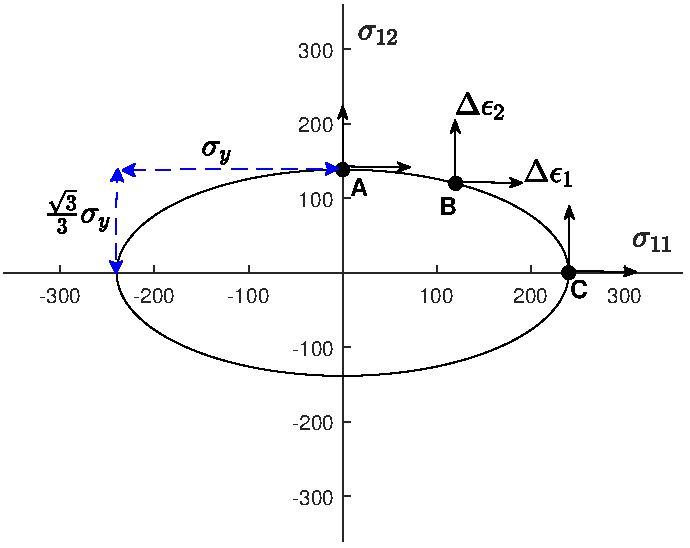
\includegraphics[scale=0.8]{FIG17_SCENARIOS}
	\caption{Points of interest on yield surface and direction of load 
		increments.}
	\label{fig:FIG17_ISO_MAP_SCENARIOS}
\end{figure}

The parameters associated with the horizontal and vertical axes, $a_1,\ a_2$, 
are defined in the following way: $a_1=\Delta\bvec{\epsilon}_1^{}/\epsilon_y$, 
$a_2=\Delta\bvec{\epsilon}_2^{}/\epsilon_y$. As  can be seen from figures 
\ref{fig:FIG18_ISO_MAPS_PERF_PLAST}, \ref{fig:FIG19_ISO_MAPS_HARD}, the 
relative error 
remains small even for quite large increments in the strain vector. Note also 
that along the semi-major and semi-minor axes, which correspond to the cases of 
pure uniaxial and pure shear states respectively, the return mapping gives the 
exact stress 
even without subincrementation. The same is true for point B when the strain 
increments are along a direction around $68^{\circ}$ with respect to $a_1$ axis.

\begin{figure}[b]
	
	\subfloat[Point A]{%
		\hspace{-0.2cm}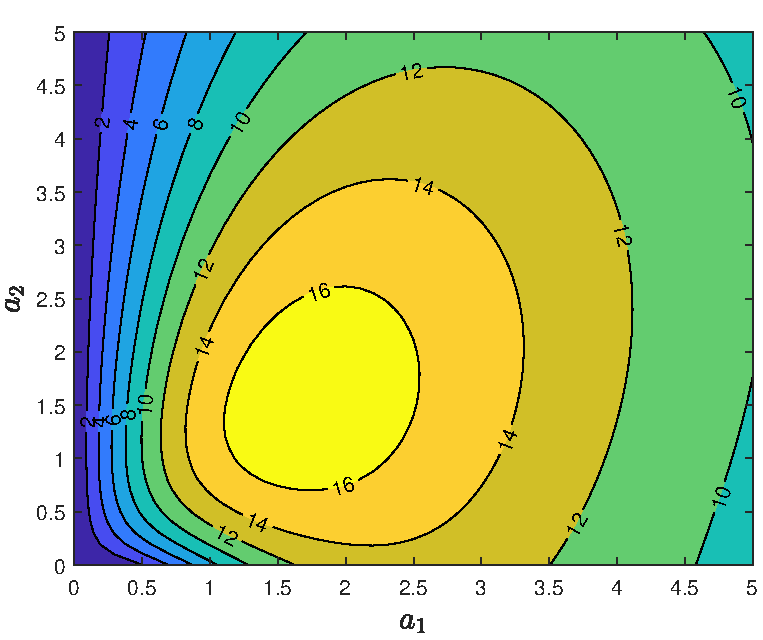
\includegraphics[width=0.33\textwidth]{FIG18_A_ISOMAP_PERF_PLAST}%
		\label{fig:FIG18_A_ISOMAP_PERF_PLAST}%
	}
	\subfloat[Point B]{%
		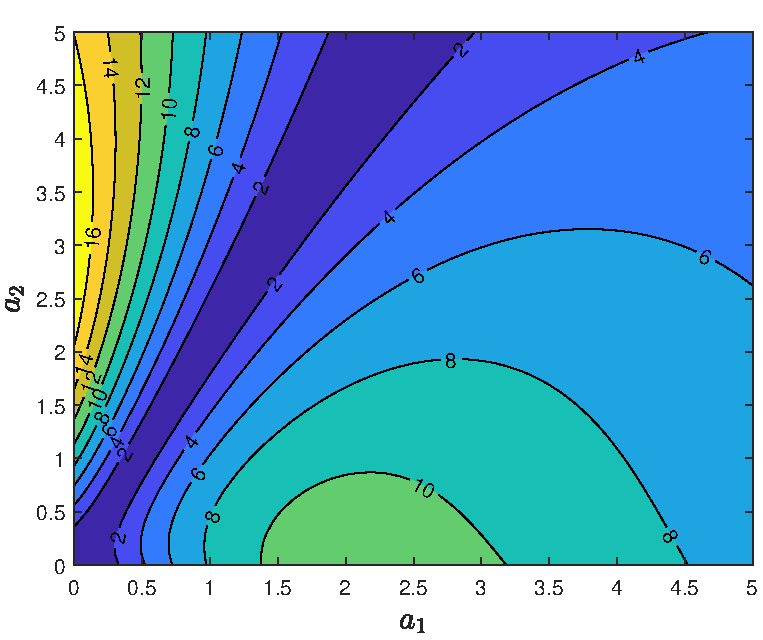
\includegraphics[width=0.33\textwidth]{FIG18_B_ISOMAP_PERF_PLAST}%
		\label{fig:FIG18_B_ISOMAP_PERF_PLAST}%
	}
	\subfloat[Point C]{%
		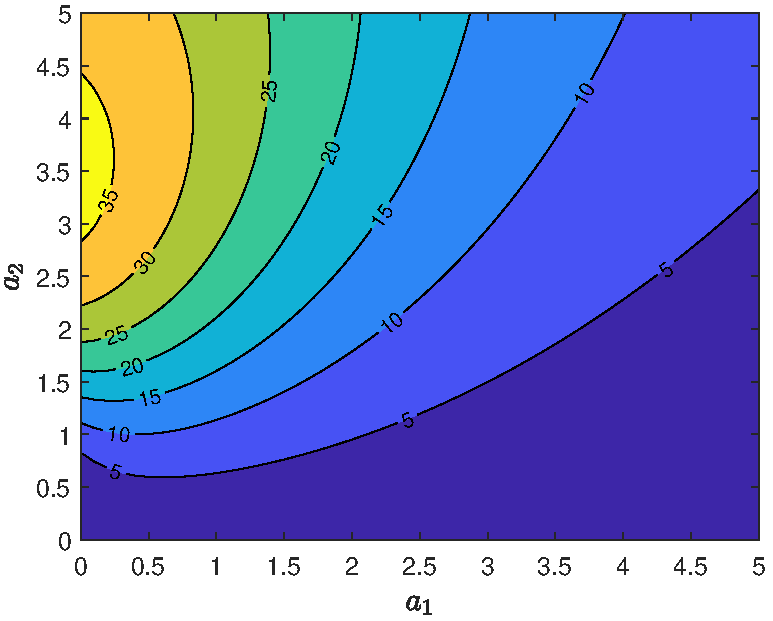
\includegraphics[width=0.33\textwidth]{FIG18_C_ISOMAP_PERF_PLAST}%
		\label{fig:FIG18_C_ISOMAP_PERF_PLAST}%
	}
	\caption{Iso-error maps for a perfectly plastic material.}
	\label{fig:FIG18_ISO_MAPS_PERF_PLAST}
\end{figure} 

\begin{figure}[t]
	
	\subfloat[Point A]{%
		\hspace{-0.2cm}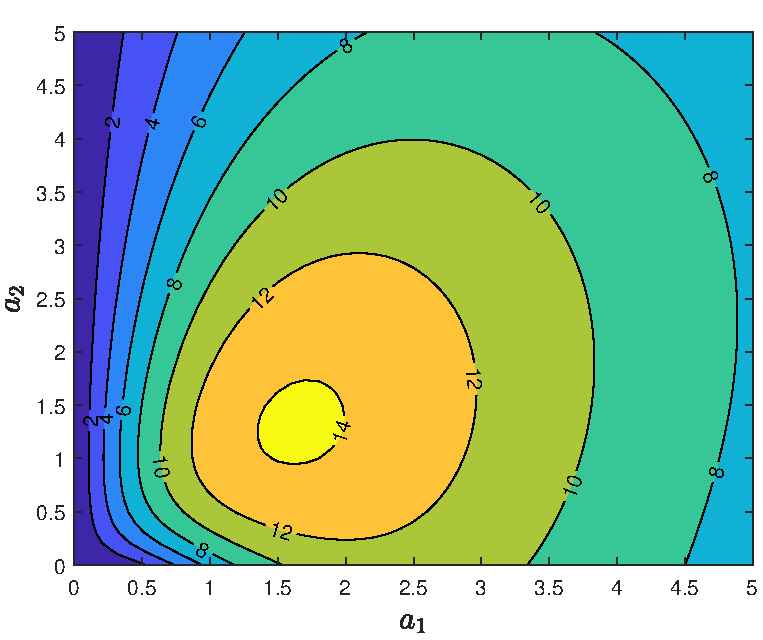
\includegraphics[width=0.33\textwidth]{FIG19_A_ISOMAP_HARD}%
		\label{fig:FIG19_A_ISOMAP_HARD}%
	}
	\subfloat[Point B]{%
		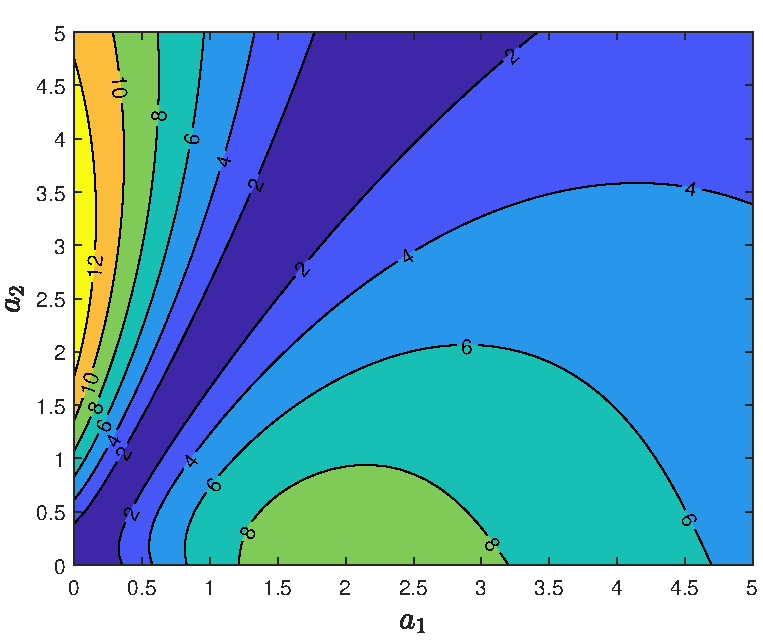
\includegraphics[width=0.33\textwidth]{FIG19_B_ISOMAP_HARD}%
		\label{fig:FIG19_B_ISOMAP_HARDT}%
	}
	\subfloat[Point C]{%
		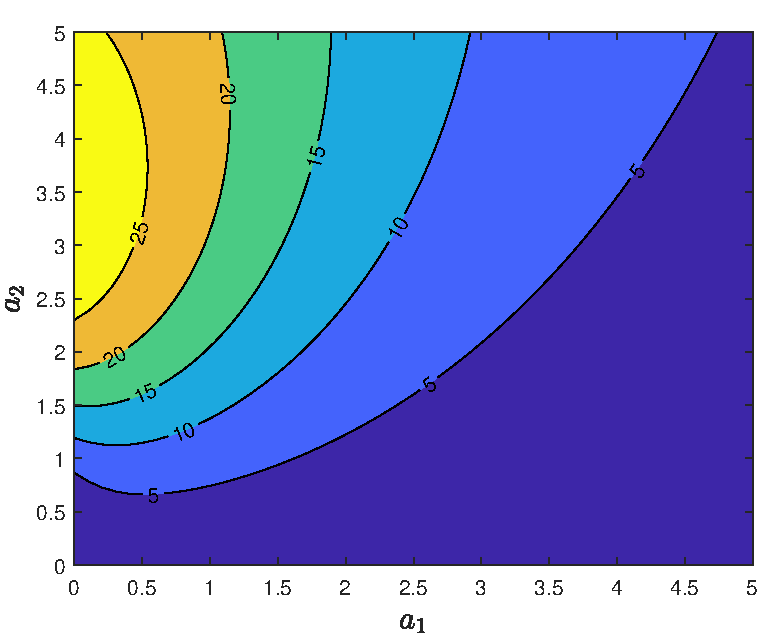
\includegraphics[width=0.33\textwidth]{FIG19_C_ISOMAP_HARD}%
		\label{fig:FIG19_C_ISOMAP_HARD}%
	}
	\caption{Iso-error maps for combined linear isotropic and kinematic 
		hardening.}
	\label{fig:FIG19_ISO_MAPS_HARD}
\end{figure} 

%%%%%%%%%%%%%%%%%%%%  EXAMPLE 2 %%%%%%%%%%%%%%%%%%%%%%%%%%%%%%%%
\subsection{Performance Against Non-Monotonic Strain Histories}

In this benchmark we investigate the performance of the proposed algorithm 
against the three dimensional/axisymmetric procedure typically implemented in 
beam elements when shear-flexure interaction is taken into account using a 
multiaxial law at the fiber level. We also compare it with the plane stress 
projection 
algorithm by Simo\cite{Simo1985}, which we followed in our derivations. In the 
former approach, the return mapping using implicit integration results in 
the so-called radial return, which doesn't require iterations in the case of 
$J_2$ with perfect plasticity or linear hardening\cite{Wilkins1963}. In 
constrast, the latter requires iterations since the topology of the stress 
space is not as simple as the von Mises cylinder anymore. We show below the 
drastic performance boost when 
using the present algorithm. As stated earlier, this is mainly due to 
the fact that we avoid an additional Newton procedure to enforce the zero 
transverse stress condition. The results for each scenario are shown in the 
tables below. A perfectly plastic material was assumed and both the average 
execution time $t$(sec) and the total number of iterations, $N_i$ are 
considered as performance metrics. All tests were performed on an Intel 
i7-7700, 3.60 GHz computer. The \textit{additional} iterations during 
purely elastic steps are also included in parentheses for the 3D and Simo's 
plane stress algorithm.  Moreover, for each scenario, four 
different incrementations of the strain history are employed, shown in Fig. 
\ref{fig:FIG20_STRAIN_HISTORIES}, and the effect of 
this scaling on the performance is highlighted. Parameter $a$ determines the 
increment ``length'': $\alpha = 
\Vert\Delta\bvec{\epsilon}\Vert^{}/\epsilon_y$. Material data are the same as 
in the previous example. 

\begin{figure}[t]
	\centering
	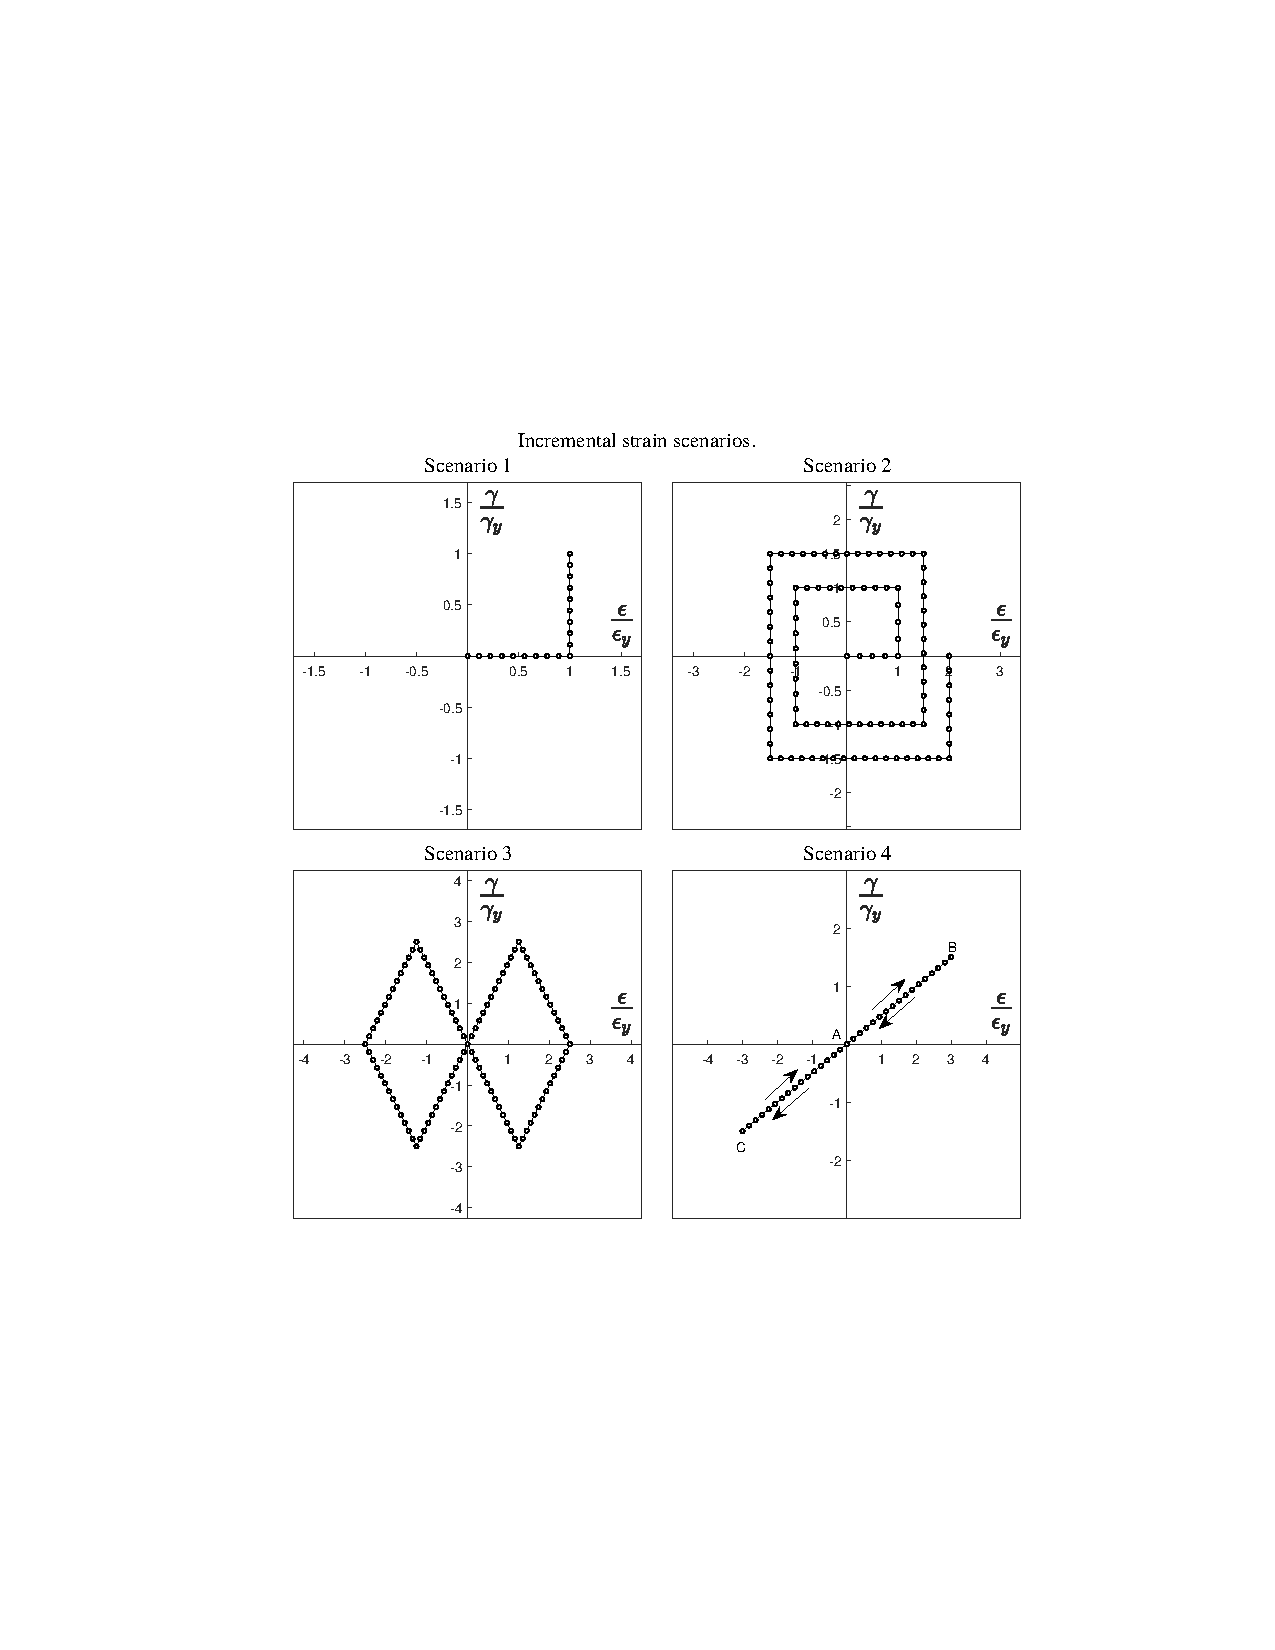
\includegraphics[scale=0.7]{FIG20_STRAIN_HISTORIES}
	\caption{The four different strain histories imposed, with the unstresses 
		configuration as initial point.}
	\label{fig:FIG20_STRAIN_HISTORIES}
\end{figure}

As can be seen from the Tables \ref{table:TABLE_1}-\ref{table:TABLE_4}, the 
proposed scheme offers significant speed-up compared to the other two methods. 
It should be highlighted that the 3D algorithm outperforms the one proposed by 
Simo because a perfectly plastic $J_2$ was used. In 
general, it too would require internal iterations to determine $\lambda$, in 
addition to the outer level Newton procedure to enforce the stress constraints. 
For Scenario 4, shown in Table \ref{table:TABLE_4}, both the 3D and plane 
stress algorithms did $[440,\ 188,\ 84,\ 62]$ elastic iterations corresponding 
to values of parameter $\alpha$: $[0.10,\ 0.25,\ 0.40,\ 0.50]$.




\begin{table}   % TABLE 1 - EXAMPLE 2
	\setlength{\tabcolsep}{9pt}
	\caption{Results for Scenario 1, perfect plasticity.}
	%	\noindent\makebox[\textwidth]{
		\begin{tabular}{@ {}lccccccccc@ {}}\toprule\toprule[0.4pt]
			Algorithm & Exact & \multicolumn{2}{c}{$\alpha=0.10$} & 
			\multicolumn{2}{c}{$\alpha=0.25$} &
			\multicolumn{2}{c}{$\alpha=0.40$}  &
			\multicolumn{2}{c}{$\alpha=0.50$}\\
			\cmidrule(r{0.60cm}l{0.40cm}){3-4} 
			\cmidrule(r{0.43cm}l{0.42cm}){5-6}
			\cmidrule(r{0.43cm}l{0.42cm}){7-8} 
			\cmidrule(r{0.10cm}l{0.45cm}){9-10}
			& $(\sigma_{11},\sigma_{12})$ & $t$\textsuperscript{a} & $N_i$ & 
			$t$ & $N_i$ & 
			$t$ & $N_i$ & $t$ & $N_i$\\
			\midrule[0.5pt]
			Proposed & {\small (1.617,1.023)} & 0.57 & 29 & 0.44 & 13 & 0.40 & 
			8 & 0.38 &  5 \\
			3D & & 1.40 & 46(20) & 0.83 & 20(8) & 0.65 & 11(4) & 0.56 
			& 6(2) \\
			Simo     &  & 1.64 & 165(19) & 1.13 & 88(7) & 0.96 & 64(3) & 0.83 & 
			55(1) \\
			\cmidrule{3-10}
			Error(\%)\textsuperscript{b}     &  & \multicolumn{2}{c}{$1.32$} & 
			\multicolumn{2}{c}{$3.00$} & \multicolumn{2}{c}{$5.16$} & 
			\multicolumn{2}{c}{$8.05$}\\
			\bottomrule\bottomrule[0.5pt]\addlinespace[3pt]
			\multicolumn{8}{l}{\textsuperscript{a} Measured in $\times 10^{-3}$ 
				sec.}\\
			\multicolumn{8}{l}{\textsuperscript{b} Relative error in converged 
				stress per increment scenario.}
		\end{tabular}
		\label{table:TABLE_1}
		%	}
\end{table}

\begin{table}   % TABLE 2 - EXAMPLE 2
	\setlength{\tabcolsep}{6.5pt}
	\caption{Results for Scenario 2, perfect plasticity.}
	%	\noindent\makebox[\textwidth]{
		\begin{tabular}{@ {}lccccccccc@ {}}\toprule[0.5pt]\toprule
			Algorithm & Exact & \multicolumn{2}{c}{$\alpha=0.10$} & 
			\multicolumn{2}{c}{$\alpha=0.25$} &
			\multicolumn{2}{c}{$\alpha=0.40$}  &
			\multicolumn{2}{c}{$\alpha=0.50$}\\
			\cmidrule(r{0.63cm}l{0.35cm}){3-4} 
			\cmidrule(r{0.63cm}l{0.40cm}){5-6}
			\cmidrule(r{0.52cm}l{0.40cm}){7-8} 
			\cmidrule(r{0.30cm}l{0.33cm}){9-10}
			& $(\sigma_{11},\sigma_{12})$ & $t$\textsuperscript{a} & $N_i$ & 
			$t$ & $N_i$ & 
			$t$ & $N_i$ & $t$ & $N_i$\\
			\midrule[0.5pt]
			Proposed & {\small (1.173,1.208)} & 0.33 & 524 & 0.16 & 234 & 0.10 
			& 144 & 0.08 & 108 \\
			3D    &                 & 1.24 & 849(97) & 0.61 & 394(40) & 0.31 
			& 196(17) & 0.23 & 143(11) \\
			Simo     &  & 2.09 & 2,791(96) & 1.17 & 1,363(39) & 0.57 
			& 790(15) & 0.42& 596(10) \\
			\cmidrule{3-10}
			Error(\%)     &  & \multicolumn{2}{c}{$2.32$} & 
			\multicolumn{2}{c}{$5.00$} & \multicolumn{2}{c}{$10.10$} & 
			\multicolumn{2}{c}{$13.35$}\\
			\bottomrule[0.5pt]\bottomrule[0.5pt]\addlinespace[3pt]
			\multicolumn{8}{l}{\textsuperscript{a} Numbers in executiont time 
				columns are measured in $\times 10^{-2}$ s.}\\
		\end{tabular}
		\label{table:TABLE_2}
		%	}
\end{table}

\begin{table}    % TABLE 3 - EXAMPLE 2
	\caption{Results for Scenario 3, perfect plasticity.}
	%\noindent\makebox[\textwidth]{
		\begin{tabular}{@ {}lccccccccc@ {}}\toprule\toprule
			Algorithm & Exact & \multicolumn{2}{c}{$\alpha=0.10$} & 
			\multicolumn{2}{c}{$\alpha=0.25$} &
			\multicolumn{2}{c}{$\alpha=0.40$}  &
			\multicolumn{2}{c}{$\alpha=0.50$}\\
			\cmidrule(r{0.65cm}l{0.30cm}){3-4} 
			\cmidrule(r{0.60cm}l{0.30cm}){5-6}
			\cmidrule(r{0.52cm}l{0.37cm}){7-8} 
			\cmidrule(r{0.33cm}l{0.30cm}){9-10}
			& $(\sigma_{11},\sigma_{12})$ & $t$\textsuperscript{a} & $N_i$ & 
			$t$ & $N_i$ & $t$ & $N_i$ & $t$ & $N_i$\\
			\midrule[0.8pt]
			Proposed & {\small (1.628,1.018)} & 0.35 & 546 & 0.16 & 237 & 0.11 
			& 147 & 0.09 &  126 \\
			3D &  & 1.15 & 920(115) & 0.61 & 405(50) & 0.31 & 194(22) & 0.29 & 
			167(16) \\
			Simo     &  & 2.20 & 2,711(114) & 1.42 & 1,307(50) & 0.55 & 789(20) 
			& 
			0.48 & 685(14) \\
			\cmidrule{3-10}
			Error(\%)     &  & \multicolumn{2}{c}{$1.15$} & 
			\multicolumn{2}{c}{$2.51$} & \multicolumn{2}{c}{$5.40$} & 
			\multicolumn{2}{c}{$5.80$}\\
			\bottomrule\bottomrule[0.5pt]\addlinespace[3pt]
			\multicolumn{8}{l}{\textsuperscript{a} Numbers in execution time 
				columns are measured in $\times 10^{-2}$ s.}
		\end{tabular}
		\label{table:TABLE_3}
		%	}
\end{table}

\begin{table}
	\setlength{\tabcolsep}{9.7pt}
	\caption{Results for Scenario 4, five cycles, perfect plasticity. One 
		cycle: A-B-C-A.}
	%\noindent\makebox[\textwidth]{
		\begin{tabular}{@ {}lccccccccc@ {}}\toprule\toprule[0.5pt]
			Algorithm & Exact &
			\multicolumn{2}{c}{$\alpha=0.10$} &
			\multicolumn{2}{c}{$\alpha=0.25$} &
			\multicolumn{2}{c}{$\alpha=0.40$} &
			\multicolumn{2}{c}{$\alpha=0.50$}\\
			\cmidrule(r{0.38cm}l{0.40cm}){3-4} 
			\cmidrule(r{0.43cm}l{0.45cm}){5-6}
			\cmidrule(r{0.43cm}l{0.45cm}){7-8} 
			\cmidrule(r{0.09cm}l{0.43cm}){9-10}
			& $(\sigma_{11},\sigma_{12})$ & $t$\textsuperscript{a} & $N_i$ & 
			$t$ & $N_i$ & $t$ & $N_i$ & $t$ & $N_i$\\
			\midrule[0.5pt]
			Proposed & {\small (2.196,0.559)} & 0.92 & 1,500 & 0.44 & 678 & 
			0.22 
			& 392 & 0.19  & 345 \\
			3D &                    & 3.50 & 2,500 & 1.61 & 1,130 & 0.77 & 490 
			& 
			0.69 & 445 \\
			Simo     &                        & 5.20 & 7,497 & 2.93 & 4,519 & 
			1.60 & 2,352 & 1.38& 2,122 \\
			\cmidrule{3-10}
			Error(\%)     &  & \multicolumn{2}{c}{$0.19$} & 
			\multicolumn{2}{c}{$0.40$} & \multicolumn{2}{c}{$0.84$} & 
			\multicolumn{2}{c}{$0.91$}\\
			\bottomrule\bottomrule[0.5pt]\addlinespace[3pt]
			\multicolumn{8}{l}{\textsuperscript{a} Numbers in execution time 
				columns are measured in $\times 10^{-2}$ s.}
		\end{tabular}
		\label{table:TABLE_4}
		
		%	}
\end{table}


%%%%%%%%%%%%%%%%%%%%  EXAMPLE 3 %%%%%%%%%%%%%%%%%%%%%%%%%%%%%%%%
\subsection{Plastic Collapse of a Doubly Clamped Beam}

In this example we investigate the collapse load of a doubly clamped beam, 
shown in Fig. \ref{fig:FIG21_CLAMPED_BEAM}, for two slenderness rations, 
$L^{}/h$: $20$ and $4$, where $h$ is 
the cross-section height. We conduct 
analysis using both uncoupled and coupled, multiaxial, constitutive models at 
the fiber level and compare result, for each case, with the lower bound 
collapse load as predicted by limit analysis.

 In addition, we showcase the 
influence of numerical quadrature in predicting the analytical solution in the 
slender case. More specifically, we compare Gauss-Legendre and Gauss-Lobatto 
quadratures. The quadrature rule used is crucial for both flexibility-based 
beam elements and the hybrid one presented and used herein, since, in both 
formulations, accuracy relies more on the precision of integration rather than 
mesh density. Lastly, each cross-section is discretized into 15 layers.

The shear strain distribution function, $k_q\varphi(X_2)$, is assumed to be 
parabolic and defined as follows:
\begin{equation}
	\varphi(X_2) = 1-4\frac{X_2^2}{h^2}
	\label{eq:SHEAR_DISTR_FUN}
\end{equation}
\noindent where $k_q$ is a parameter introduced in order to establish shear 
strain energy equivalence between assumed and exact distributions. For that 
matter, it is convenient to consider the uniform shear strain-average force 
hypothesis coupled with the corresponding shear coefficient as a representation 
of the exact one, assuming elastic behavior:
\begin{equation}
	\mathcal{U}_{shear}^{exact}=k_s\mathcal{U}_{shear}^{unif} = 
	k_q\mathcal{U}_{shear}^{quad}\Longleftrightarrow 
	\frac{1}{2}k_sGA\gamma ^2=\frac{1}{2}G k_q^2\bigg(\int_A \varphi(X_2)^2 dA 
	\bigg) \gamma ^2
	\label{eq:SHEAR_COEFF}
\end{equation}
\noindent where $k_s$ is the shear coefficient for uniform shear strain 
assumption. For rectangular sections with $\nu=0.3$, 
$k_s=0.886$ and solving eq. (\ref{eq:SHEAR_COEFF}) for $k_q$ we 
get:
\begin{equation}
	k_q = \sqrt{\frac{k_s A}{\int_A \varphi(X_2)^2 dA}}
	\label{eq:QUAD_COEFF}
\end{equation}

A first observation from Fig. \ref{fig:FIG22_EQUILIBRIUM_PATHS} is that 
Gauss-Legendre quadrature tends to overestimate the capacity load on both edges 
of the slenderness spectrum. Gauss-Lobatto quadrature, in contrast, is 
more accurate and converges to the ``exact'' capacity from ``below''. In 
addition, it provides accuracy with just five quadrature points whereas even 
with nine points, Gauss-Legendre still is not as accurate and converges from 
``above''. 
The results are in agreement with the ones reported by Papachristidis et 
al.\cite{Papachristidis2010} in a similar investigation.

When it comes to the influence of slenderness in the plastic capacity, the 
collapse 
load for the $L^{}/h=4$ case predicted by the multiaxial constitutive law is 
lower than the one based on limit analysis. Interestingly, the uncoupled 
constitutive law results in a purely flexural collapse mode, thus yielding a 
ultimate load coinciding with the theoretical from limit analysis. When the 
beam is slender, both coupled and uncoupled constitutive laws result, 
expectably, in a flexure-dominant mode. 

\begin{figure}[t]
	\centering
	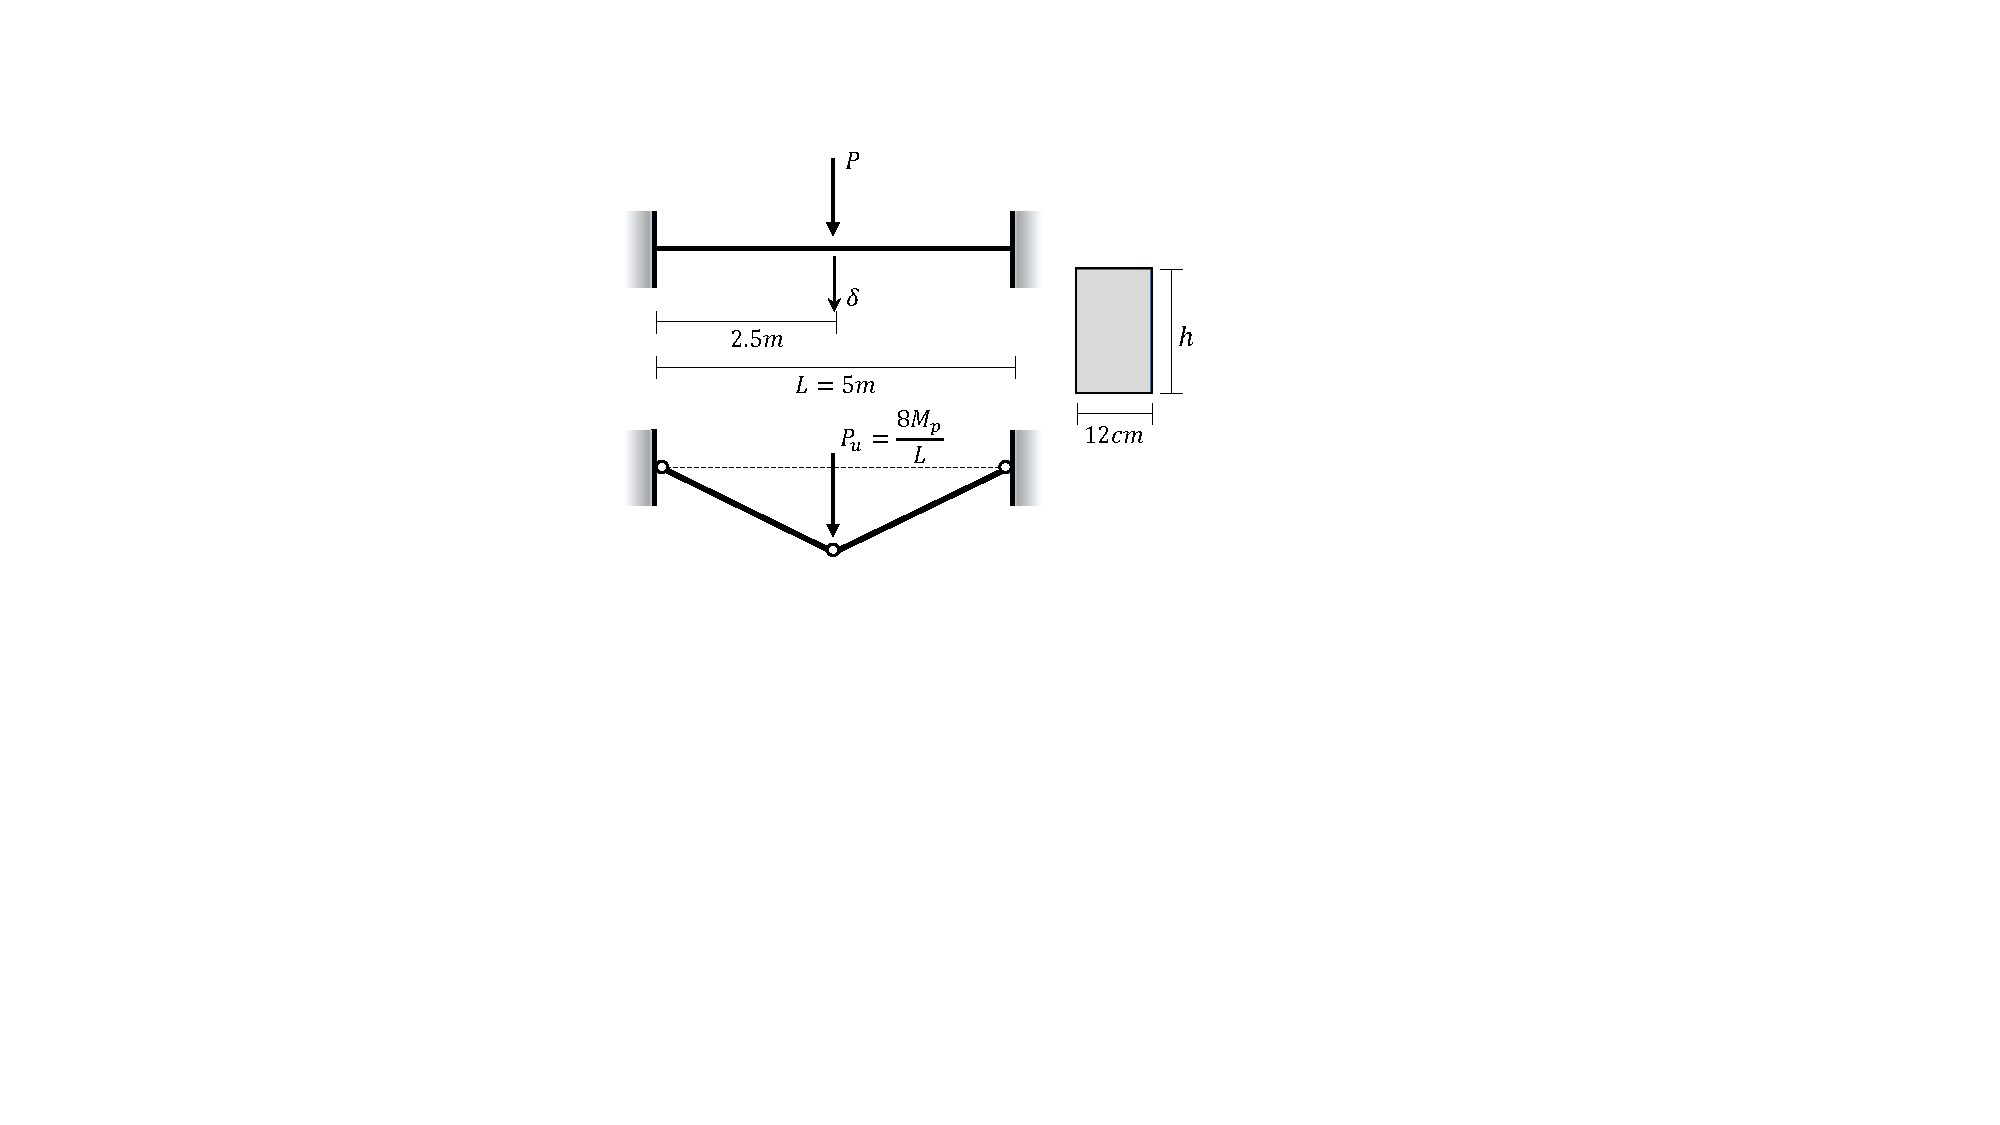
\includegraphics[scale=0.7]{FIG21_CLAMPED_BEAM}
	\caption{Geometry, initial and final configuration of clamped beam, along 
		with cross-section dimensions.}
	\label{fig:FIG21_CLAMPED_BEAM}
\end{figure}

The results are summarized in Table 
\ref{table:TABLE_5} and Fig. \ref{fig:FIG22_EQUILIBRIUM_PATHS}. In Fig. 
\ref{fig:FIG23} the stress distributions for $\sigma_{11}$, $\sigma_{12}$ and 
the von Mises stress, $\sigma_{VM}=\sqrt{3J_2}$ are presented at three 
different load levels indicated by points A, B and C (see Fig. 
\ref{fig:FIG22_B}). 
The plastic zone propagation is also exhibited. While the von Mises and Plastic 
Zone (P.Z.)
profiles resemble plastification profiles typical of flexure-dominant members, 
we observe that the lower 
capacity captured by the multiaxial model in the $L^{}/h=4$ case, which Fig. 
\ref{fig:FIG23} pertains to, is due to shear plastification of the shrinking 
elastic core, a phenomenon which is neglected in a purely uniaxial formulation.

\begin{figure}
	\centering
	\subfloat[$L^{}/h=20$]{%
		\hspace{-0.2cm}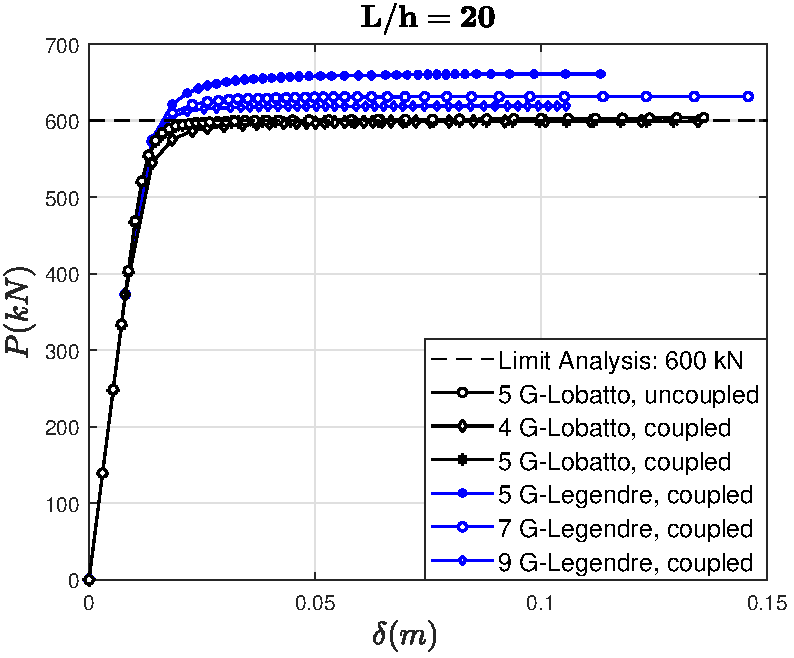
\includegraphics[width=0.45\textwidth]{FIG22_A_CLAMPED_LH20}%
		\label{fig:FIG22_A}%
	}
	\subfloat[$L^{}/h=4$]{%
		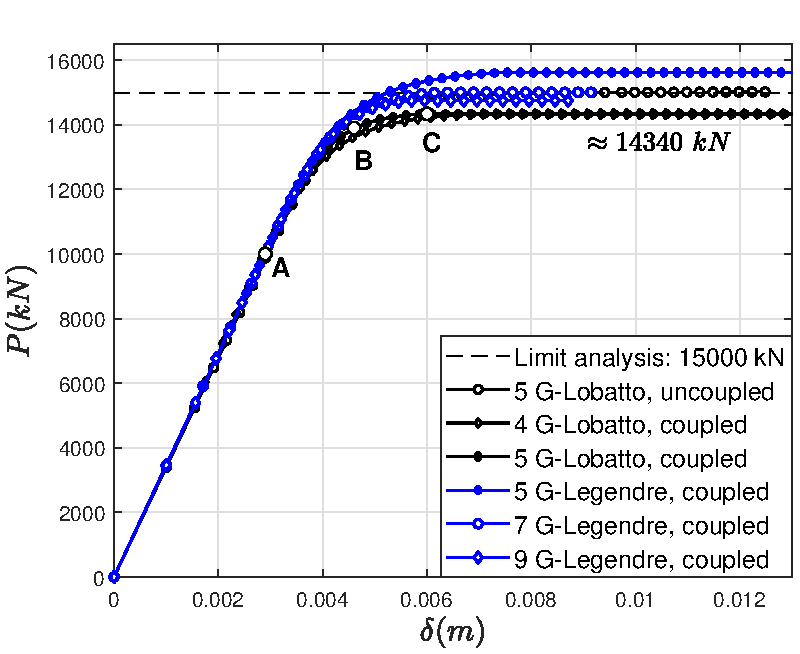
\includegraphics[width=0.45\textwidth]{FIG22_B_CLAMPED_LH4}%
		\label{fig:FIG22_B}%
	}
	\caption{Load-deflection plots for different slenderness ratios. Influence 
		of quadrature type and number of points.}
	\label{fig:FIG22_EQUILIBRIUM_PATHS}
\end{figure} 

\clearpage

\noindent\makebox[\textwidth][c]{
	\begin{minipage}{0.7\textwidth}
		\vskip15pt
		\captionof{table}{Collapse moments and loads for clamped beam.}
		\begin{tabular}{@ {}ccccc@ 
				{}}\toprule[0.4pt]\toprule[0.4pt]\addlinespace[-2pt]
			&  & \multicolumn{3}{c}{Collapse load, 
				$P_u(kN)$\textsuperscript{a}}\\ 
			\cmidrule{3-5}
			$L^{}/h$ & $M_p(kN\cdot m)$ & Limit Analysis & Uncoupled & Coupled\\
			\midrule[0.5pt]\addlinespace[-2pt]
			$20$ & $3.75\cdot 10^2$ & $6.00\cdot 10^2$ & $\approx 6.00\cdot 
			10^2$ & $\approx 6.00\cdot 10^2$\\ \addlinespace[-2pt]
			$4$  & $9.37\cdot 10^3$ & $1.50\cdot 10^4$ & $\approx 1.50\cdot 
			10^4$ & $\approx 1.43\cdot 10^4$\\ \addlinespace[-2pt]
			\bottomrule[0.4pt]\bottomrule[0.4pt]\addlinespace[-3pt]
			\multicolumn{5}{l}{\small Material data: $E=200\ GPa$, 
				$\sigma_y=200\ 
				MPa$.}\\ \addlinespace[-9pt]
			\multicolumn{5}{l}{\textsuperscript{a} \small For coupled and 
				uncoupled loads, 5 Gauss-Lobatto points are assumed.}
		\end{tabular}
		
		\label{table:TABLE_5}
	\end{minipage}
}

\begin{figure}
	\centering
	\setlength\tabcolsep{1pt}
	%\settowidth\rotheadsize{Plastification}
	\begin{tabular}{c|ccc}
		& \textbf{A} : $P=10,000\ kN$  & \textbf{B} : $P=13,900\ 
		kN$              
		& \textbf{C} : $P = 14,340\ kN$\\
		\midrule
		P.Z.         & \sprofs{FIG23_PlastP10000.pdf}     & 
		\sprofs{FIG23_PlastP13900.pdf}     & \sprofs{FIG23_PlastP14340.pdf}\\
		$\sigma_{VM}$& \sprofs{FIG23_PlastP10000_VM.pdf}  & 
		\sprofs{FIG23_PlastP13900_VM.pdf}  & \sprofs{FIG23_PlastP14340_VM.pdf}\\
		$\sigma_{11}$     & \sprofs{FIG23_PlastP10000_SXX.pdf} & 
		\sprofs{FIG23_PlastP13900_SXX.pdf} & 
		\sprofs{FIG23_PlastP14340_SXX.pdf}\\
		$\sigma_{12}$       & \sprofs{FIG23_PlastP10000_SXY.pdf} & 
		\sprofs{FIG23_PlastP13900_SXY.pdf} & \sprofs{FIG23_PlastP14340_SXY.pdf}
	\end{tabular}
	\caption{Case $L^{}/h=4$. Spread of Plastic Zone (P.Z.) and stress 
		distribution for von 
		Mises, axial and shear stress at three different load levels.}
	\label{fig:FIG23}
\end{figure}

%%%%%%%%%%%%%%%%%%%%  EXAMPLE 4 %%%%%%%%%%%%%%%%%%%%%%%%%%%%%%%%
\subsection{Cyclic Loading of Shear Link}\label{CH3EX4}

In this example we are examining the response of a metallic shear link 
(Fig.\ref{fig:FIG24A}) 
with a symmetric wide flange cross-section under displacement-controlled cyclic 
loading. The specimen we are concerned with was part of an experimental 
investigation by Hjelmstad \& Popov\cite{Hjelmstad1983} and later was 
numerically analyzed by Saritas \& Filippou\cite{Saritas2009} using a mixed 
beam element formulation with shear-flexure interaction at the fiber level. In 
our analsys the specimen was modelled using one hybrid element with five 
Gauss-Lobatto points and 21 layers at each section with three layers on each 
flange. 

\begin{figure}[H]
	\centering
	\subfloat[Structure.]{
		\begin{minipage}[c]{0.4\linewidth}
			%\captionsetup{type=figure}
			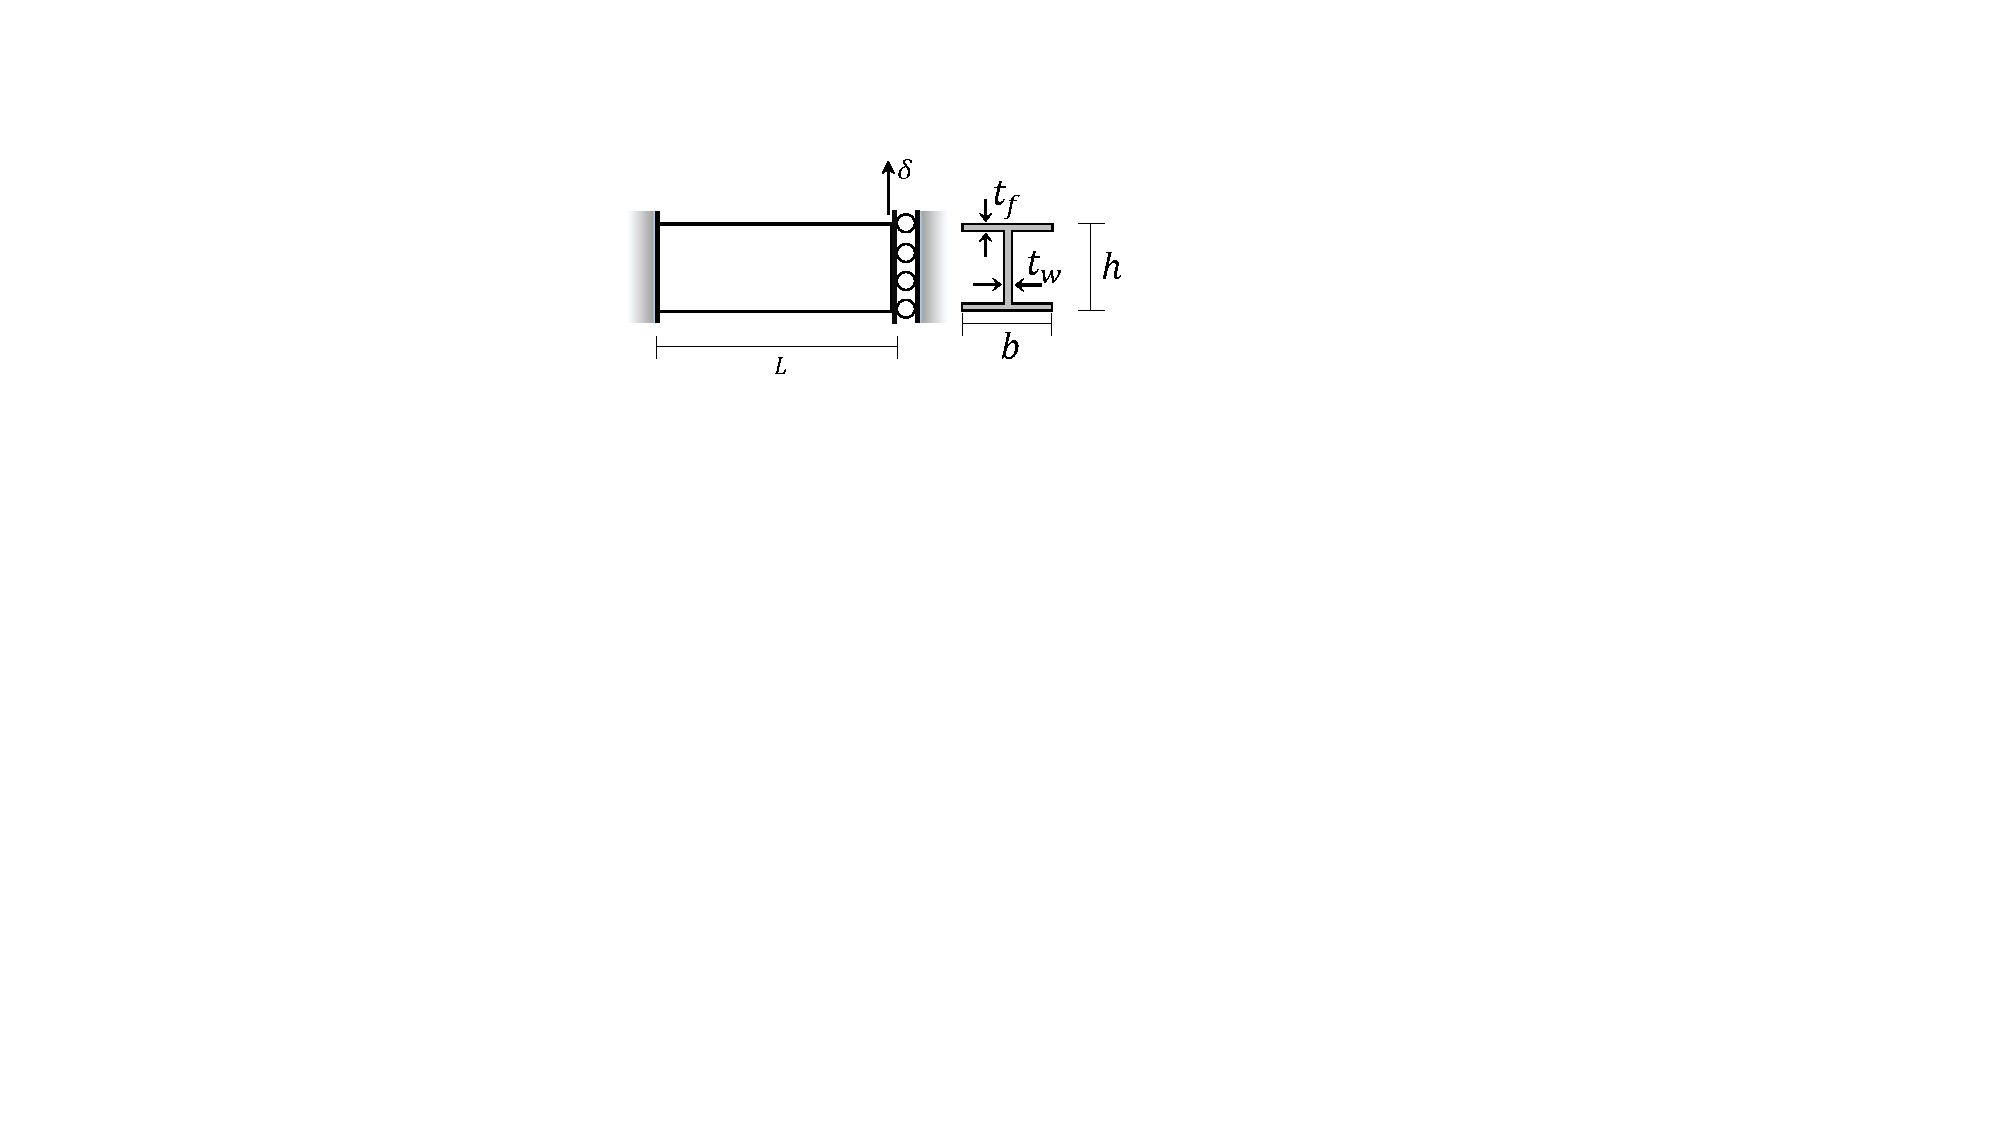
\includegraphics[scale=0.8]{FIG24_Structure}%
			%\caption{Structure.}
			\label{fig:FIG24A}%
		\end{minipage}
	}
	%\subfloat[Structure.]{%
		%	
		%\hspace{-0.2cm}\includegraphics[width=0.45\textwidth]{FIG11_Structure}%
		%	\label{fig:FIG11A}%
		%	}
	\subfloat[Displacement-controlled loading history.]{%
		\hspace{0.3cm}\begin{minipage}{0.55\linewidth}
			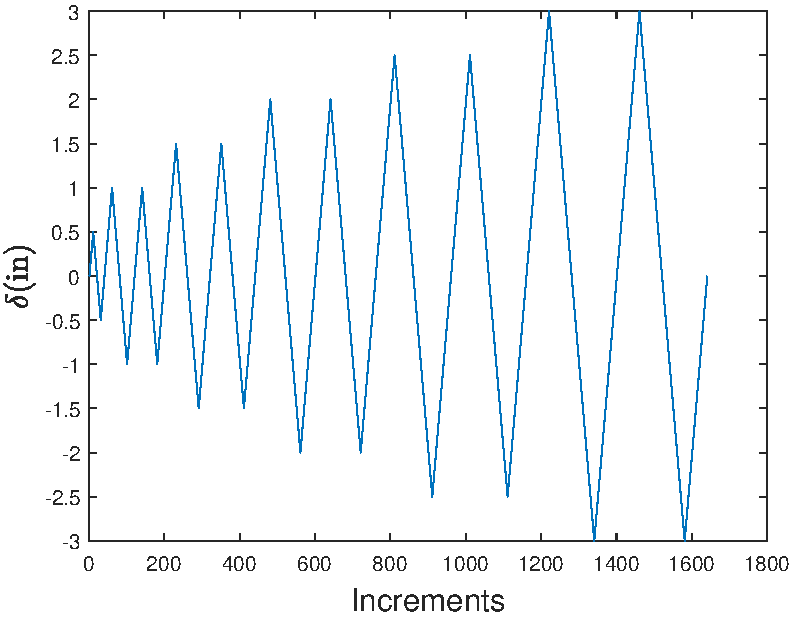
\includegraphics[scale=0.6]{FIG24_DISPHIST}%
			\label{fig:FIG24B}%
		\end{minipage}
		%\includegraphics[width=0.45\textwidth]{FIG11_DISPHIST}%
		%\label{fig:FIG11B}%
	}
	\caption{Geometry of the specimen and displacement-controlled loading 
		history.}
	\label{fig:FIG24}
\end{figure}

The specimen length is $L=28$ in. and the cross-section type is W $18\times40$ 
with basic dimensions 
specified as follows: total height $h=17.88$ in., flange width $b=5.985$ in., 
web and flange thickness, $t_w=0.314$ in. and $t_f=0.521$ in. respectively. The 
material properties are summarized in Table \ref{table:TABLE6}, while the 
displacement history, in 
accordance with Hjelmstad \& Popov's experiment, is shown in 
Fig.\ref{fig:FIG24B}. 


 As can be seen in Fig. \ref{fig:FIG25}, satisfactory agreement with the 
 experimental results is achieved when setting 
$H_{kin}=78.4$ kips/in${}^2$ and $H_{iso} = 8.40$ kips/in${}^2$ and assuming 
a quadratic shear strain distribution along the cross-section height, in 
accordance with the previous example. More specifically, it was found that 
better agreement with the experimental results was achieved by sligtly 
increasing the shear factor $k_q$ to $1.62$ from the default value of $1.33$, 
as determined by eq. (\ref{eq:QUAD_COEFF}). The main cause for the discrepancy 
is that with the procedure outlined in Example 3 for the determination of the 
equivalent ``quadratic'' shear coefficient, an assumption for the shear stress 
distribution is not considered and this can be a source of non-negligible 
inaccuracies when open thin-walled sections are used. Nevertheless, since 
neither the distribution of shear fields on the cross-section shapes nor the 
particularization of flow and hardening laws for cyclic loading are the main 
focus of this study, some inaccuracies during cyclic plastification are to be 
expected and tolerated. In addition, a slight divergence during the unloading 
phases can be observed between the numerical and experimental tests. As 
explained in \cite{Saritas2009}, this is due to 
improper restraint of the specimen during the experiment.

 

\begin{figure}[H]
	\centering
	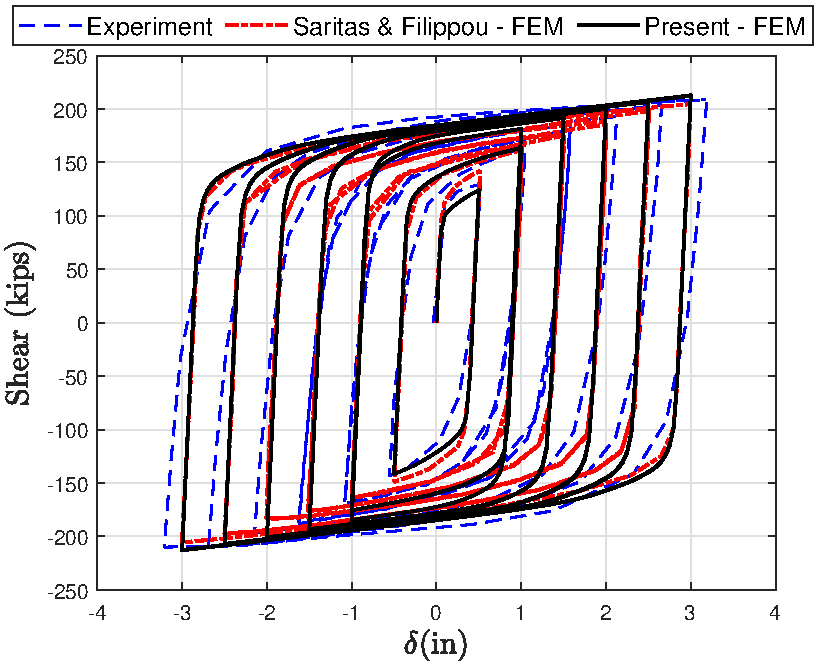
\includegraphics[scale=0.65]{FIG25_HISTORIES}
	\caption{Experimental and numerical results for the specimen.}
	\label{fig:FIG25}
\end{figure}

\begin{table}
	\centering
	\begin{minipage}{0.8\linewidth}
		\caption{Material properties for Example \ref{CH3EX4}.}
		\begin{tabular}{ccccccc}
			\toprule\toprule
			\vtop{\hbox{\strut \hspace{.25cm}Section}\hbox{\strut W 
			$18\times40$}} 
			& \vtop{\hbox{\strut \hspace{0.5cm}$\sigma_y$}\hbox{\strut 
					($\text{kips}^{}/\text{in}^2$)}}  &         
					\vtop{\hbox{\strut 
					\hspace{0.5cm}$\sigma_u$}\hbox{\strut 
					($\text{kips}^{}/\text{in}^2$)}} &
			\vtop{\hbox{\strut \hspace{2.5pt}$\epsilon_y$}\hbox{\strut (\%)}} & 
			\vtop{\hbox{\strut \hspace{2.5pt}$\epsilon_u$}\hbox{\strut (\%)}} 
			&\vtop{\hbox{\strut \hspace{0.5cm}$E$}\hbox{\strut 
					($\text{kips}^{}/\text{in}^2$)}} & \vtop{\hbox{\strut 
					\hspace{0.4cm}$H_{kin}$}\hbox{\strut 
					($\text{kips}^{}/\text{in}^2$)}} \\
			\midrule
			Web & 39.5 & 60.1 & 1.8 & 22 & 28,300 & 102 \\
			Flange & 35.0 & 58.5 & 1.4 & 24 & 28,000 & 102\\
			\bottomrule\bottomrule
		\end{tabular}
		\label{table:TABLE6}
	\end{minipage}
\end{table}

\begin{figure}[H]
	\centering
	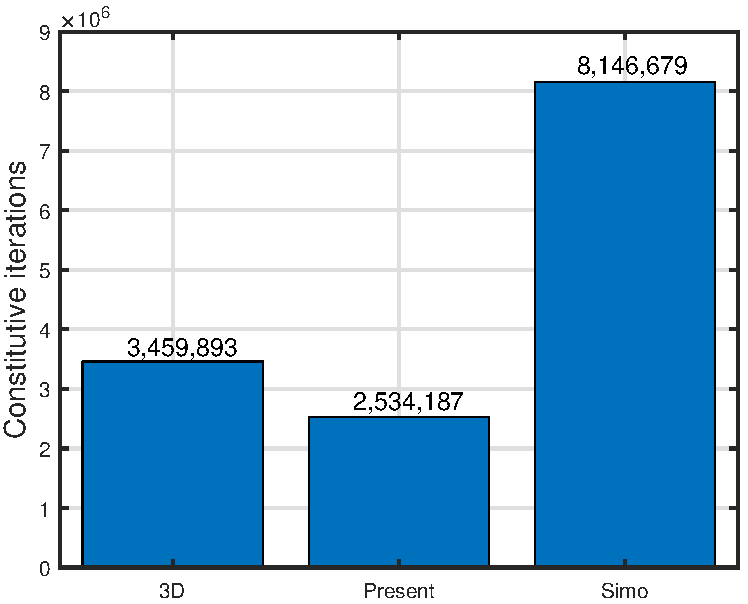
\includegraphics[scale=0.6]{FIG_BARS}
	\caption{Performance of the three different return-mapping algorithms 
		applied for the section state determination of the shear link under the 
		imposed displacement history.}
	\label{fig:FIG_BARS}
\end{figure}

\clearpage

Performance analysis of the three different return-mapping schemes is also 
conducted for this example, where now we will examine the total number of 
constitutive iterations during the whole history of the imposed displacement. 
This helps highlight the significant acceleration the proposed algorithm offers 
during a more complex analysis that involves nonlinear response of an element 
comprised of multiple sections, each of which is discretized in several 
layers. The results when we use the three-dimensional/axisymmetric, Simo's 
plane stress and the proposed algorithm are shown in Fig. \ref{fig:FIG_BARS}. 
As mentioned earlier, the linear hardening constitutive model even tends to 
favor the 
three-dimensional algorithm since the plastic correction reduces to the 
so-called radial return. However, in a 
more general setting where nonlinear hardening or a different material model is 
used, the performance differentials between the proposed scheme and its 
three-dimensional counterpart would be even more pronounced.

%%%%%%%%%%%%%%%%%%%%  EXAMPLE 5 %%%%%%%%%%%%%%%%%%%%%%%%%%%%%%%%
\subsection{Elastoplastic Post-Buckling Behavior of Two-Beam Structure}

This problem has been previously analyzed in \cite{Argyris1982,Ridha1971}. The 
structure, shown in Fig. \ref{fig:FIG26_STRUCTURE}, enters its inelastic regime 
immediately after the buckling 
load is reached, whereby point B starts moving inwards. In 
Fig. \ref{fig:FIG26_COMPARISON} we compare the 
results we get using just three hybrid elements and five Gauss-Lobatto points 
in each 
element with the ones of Argyris et al.\cite{Argyris1982}. In addition, we 
include the 
inelastic analysis, which demonstrates that plastification starts immediately 
after the instability. Material and geometric data are shown in 
Table \ref{table:TABLE7}. Again, we highlight the impact of a coupled 
multiaxial law by 
investigating a variation of this problem. For all cases, inelastic response 
with kinematic hardening is assumed. 



\begin{table}
	\centering
 	\begin{minipage}{0.7\textwidth}
 		%\vskip-10pt
 		\caption{Member geometric and material data.}
 		\label{table:TABLE7}
 		\begin{tabular}{@ {}ccccccc@ {}}\toprule\toprule
 			Member & $E (\frac{\text{kN}}{\text{cm}^2})$ & 
 			$H_{kin}(\frac{\text{kN}}{\text{cm}^2})$ & 
 			$\sigma_y(\frac{\text{kN}}{\text{cm}^2})$ & $h_s(\text{cm})$ & 
 			$h_t(\text{cm})$ & $b(\text{cm})$\\
 			\midrule[0.5pt]
 			\circled{1} & $6.86\times 10^3$ & $2.84\times 10^2$ & $26.20$ & 
 			$1.91$ & $8.00$ & $2.54$ \\ \addlinespace[3pt]
 			\circled{2} & $6.86\times 10^3$ & $2.84\times 10^2$ & $33.10$ & 
 			$1.91$ & $8.00$ & $2.54$ \\
 			\bottomrule\bottomrule[0.5pt]\addlinespace[3pt]
 		\end{tabular}
 	\end{minipage}
\end{table}

\begin{figure}[t]
	\centering
	\subfloat[Structure.]{%
		\hspace{-0.2cm}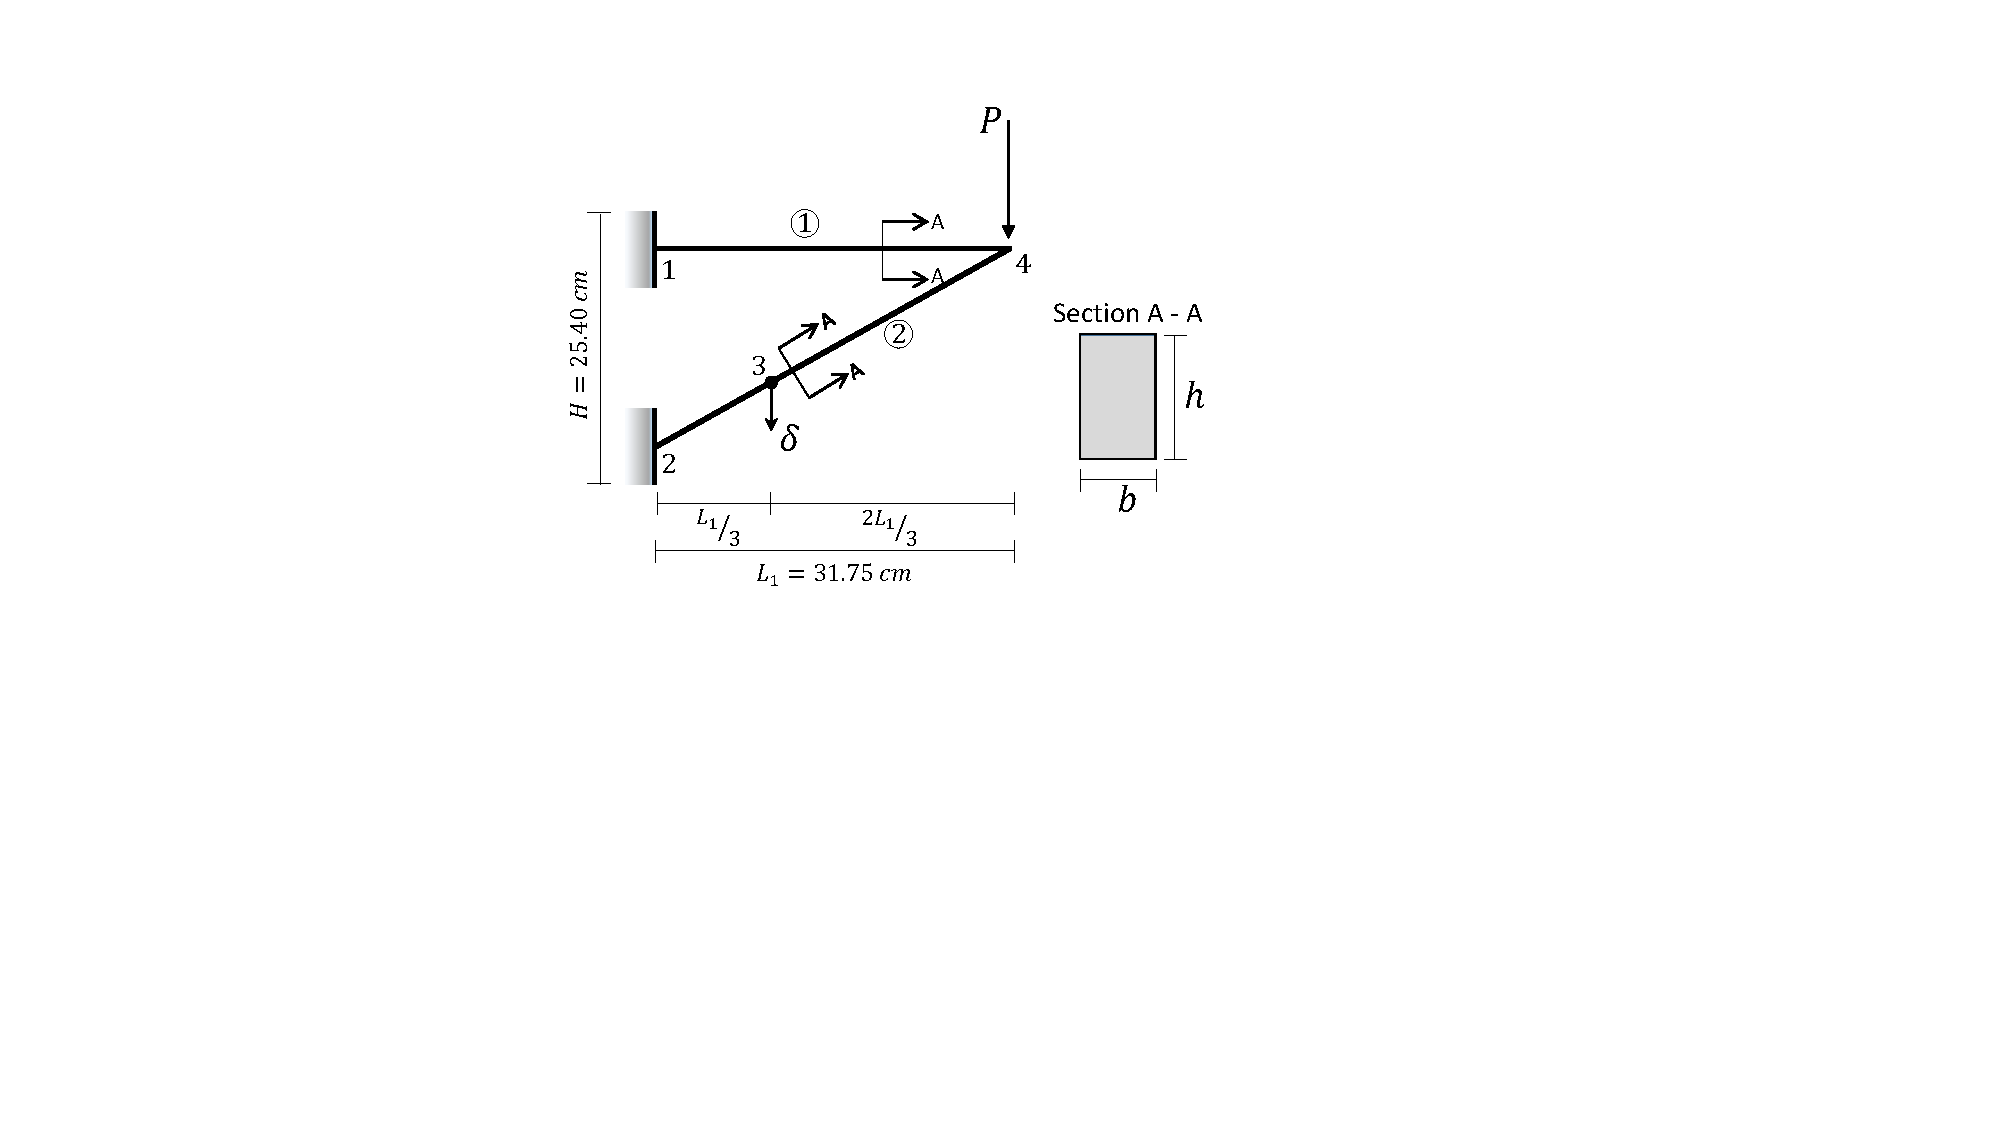
\includegraphics[width=0.45\textwidth]{FIG26_A_STRUCTURE}%
		\label{fig:FIG26_STRUCTURE}%
	}
	\subfloat[Load vs deflection $\delta$ at point 3.]{%
		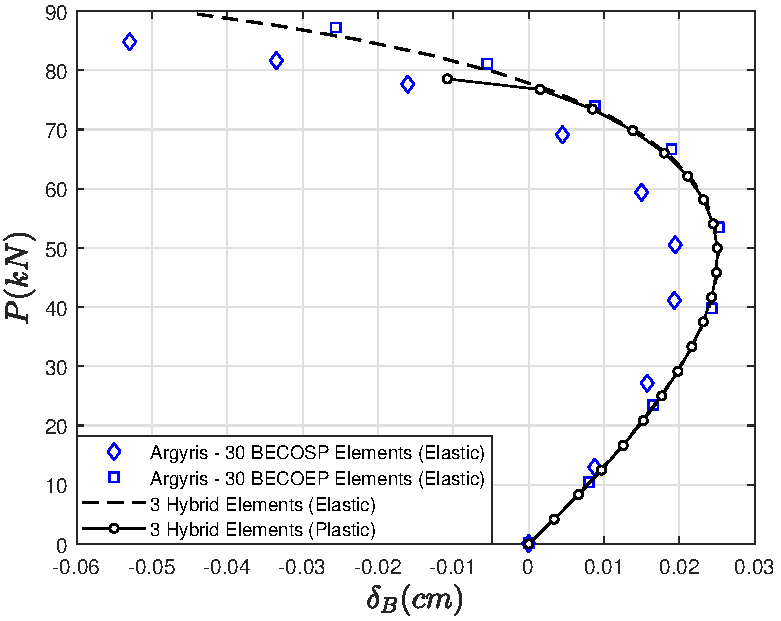
\includegraphics[width=0.45\textwidth]{FIG26_B_COMPARISON}%
		\label{fig:FIG26_COMPARISON}%
	}
	\caption{Geometry and loading of two-beam structure. Comparison of load vs 
		deflection curves for different cases.}
	\label{fig:FIG26}
\end{figure} 



\begin{figure}[b]
	\centering
	\subfloat[Elastic.]{%
		\hspace{-0.2cm}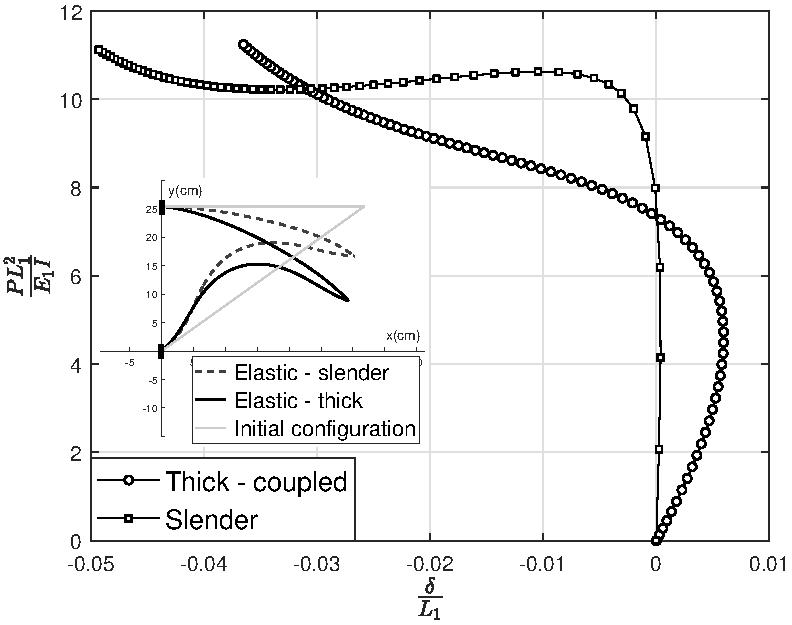
\includegraphics[width=0.45\textwidth]{FIG27_A_ELASTIC_COMPARISON}%
		\label{fig:FIG27_ELASTIC}%
	}
	\subfloat[Plastic.]{%
		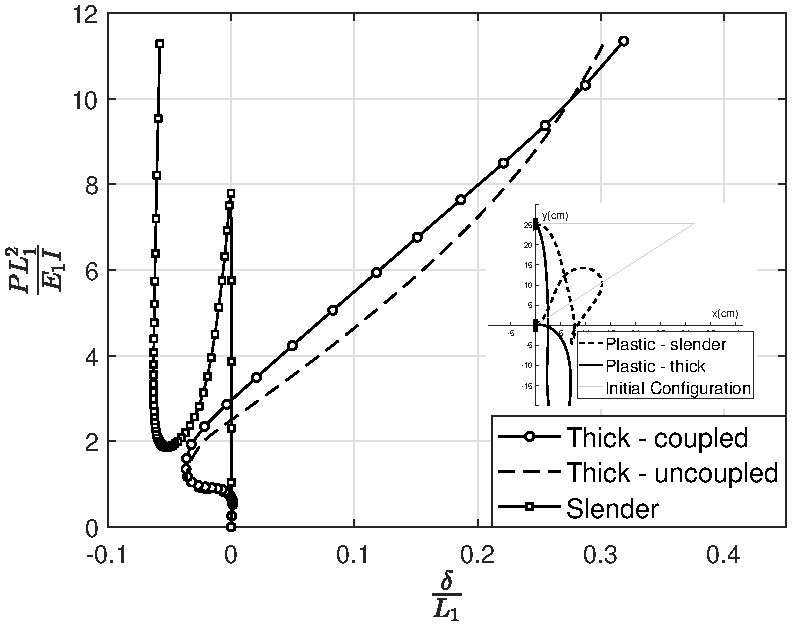
\includegraphics[width=0.45\textwidth]{FIG27_B_PLASTIC_COMPARISON}%
		\label{fig:FIG27_PLASTIC}%
	}
	\caption{Influence of slenderness and constitutive model on the response 
		for elastic and elastoplastic behavior.}
	\label{fig:FIG27}
\end{figure}

\clearpage
Convergence data in residual norm and 
energy norms for the case of thick members are also shown in Tables 
\ref{table:TABLE8}, \ref{table:TABLE9} for selected steps. In Fig. 
\ref{fig:RATES} we also show 
plots of convergence rates for the global Newton method when using the 
consistent and continuous tangent respectively for two representative steps. It 
is evident that use of the continuous tangent modulus slows down convergence 
significantly.
%% RESIDUAL NORM
\begin{table}
	\centering
	\begin{minipage}{0.9\linewidth}
		\caption{Convergence in residual norm during steps 5, 15, 25 35. 
			$\mathcal{\epsilon}_{tol}=10^{-10}$.}
		\label{table:TABLE8}
		\begin{tabular}{@ {}cllll@ {}}\toprule\toprule
			iterations & \hspace{0.8cm} 
			5 & \hspace{0.7cm} 15 & \hspace{0.7cm} 25 & \hspace{0.8cm} 35 \\
			\midrule
			1 & $1.000000\cdot 10^0$     & $1.000000\cdot 10^0$     & 
			$1.000000\cdot 10^0$     & $1.000000\cdot 10^0$ \\
			2 & $1.251499\cdot 10^{-2}$  & $1.988783\cdot 10^{-2}$ & 
			$1.737845\cdot 10^{-3}$  & $6.187773\cdot 10^{-2}$ \\
			3 & $2.132711\cdot 10^{-5}$  & $1.066255\cdot 10^{-5}$ & 
			$1.824164\cdot 10^{-6}$  & $4.214041\cdot 10^{-3}$ \\
			4 & $9.483080\cdot 10^{-10}$ & $4.882520\cdot 10^{-10}$ & 
			$2.229120\cdot 10^{-11}$ & $6.111545\cdot 10^{-5}$ \\
			5 & $5.150000\cdot 10^{-14}$ & $7.790000\cdot 10^{-13}$ & 
			$4.800000\cdot 10^{-14}$ & $1.218231\cdot 10^{-8}$  \\
			6 &  & &  & $7.110000\cdot 10^{-14}$\\
			\bottomrule\bottomrule[0.5pt] %\addlinespace[3pt]
		\end{tabular}
	\end{minipage}
\end{table}
\begin{table}%% ENERGY NORM 
	\centering
	\begin{minipage}{0.9\linewidth}
		\caption{Convergence in energy norm during steps 5, 15, 25, 35.%
			$\ \mathcal{\epsilon}_{tol}=10^{-10}$.}
		\label{table:TABLE9}
		\begin{tabular}{@ {}cllll@ {}}\toprule\toprule
			iterations  & 
			\hspace{0.8cm} 5 & \hspace{0.7cm} 15 & \hspace{0.7cm} 25 & 
			\hspace{0.8cm} 35 \\
			\midrule
			1 & $1.000000\cdot 10^0$    &  $1.000000\cdot 10^0$  & 
			$1.000000\cdot 10^0$ & $1.000000\cdot 10^0$ \\
			2 & $3.050574\cdot 10^{-4}$  &  $1.065944\cdot 10^{-4}$ & 
			$2.618542\cdot 10^{-2}$ & $1.188951\cdot 10^{-2}$ \\
			3 & $2.235712\cdot 10^{-5}$  &  $5.373434\cdot 10^{-5}$ & 
			$4.974768\cdot 10^{-5}$ & $1.495507\cdot 10^{-4}$ \\
			4 & $1.532842\cdot 10^{-8}$  &  $2.585263\cdot 10^{-9}$ & 
			$1.551550\cdot 10^{-7}$ & $1.706384\cdot 10^{-5}$ \\
			5 & $6.283000\cdot 10^{-12}$ &  $1.962000\cdot 10^{-12}$ & 
			$1.687900\cdot 10^{-11}$ & $3.948037\cdot 10^{-7}$  \\
			7 &  & &  & $5.157400\cdot 10^{-11}$ \\
			\bottomrule\bottomrule[0.5pt] %\addlinespace[3pt]
		\end{tabular}
	\end{minipage}
\end{table}


As can be seen from 
Fig. \ref{fig:FIG27_PLASTIC} for the inelastic analysis of 
the thick member variation, the equilibrium paths corresponding to a coupled 
and uncoupled constitutive law tend to diverge shortly after the start of 
plastic deformation.

The full post-buckling elastoplastic equilibrium curve for 
the slender model is also provided for comparison. In 
Fig. \ref{fig:FIG27_ELASTIC} the post-buckling response of both slender and 
thick 
models are illustrated. In the former, both uniaxial and multiaxial 
constitutive models yield identical results, assuming an infinite yield stress.


\begin{figure}[t]
	\centering
	\subfloat[Step 15.]{%
		\hspace{-0.2cm}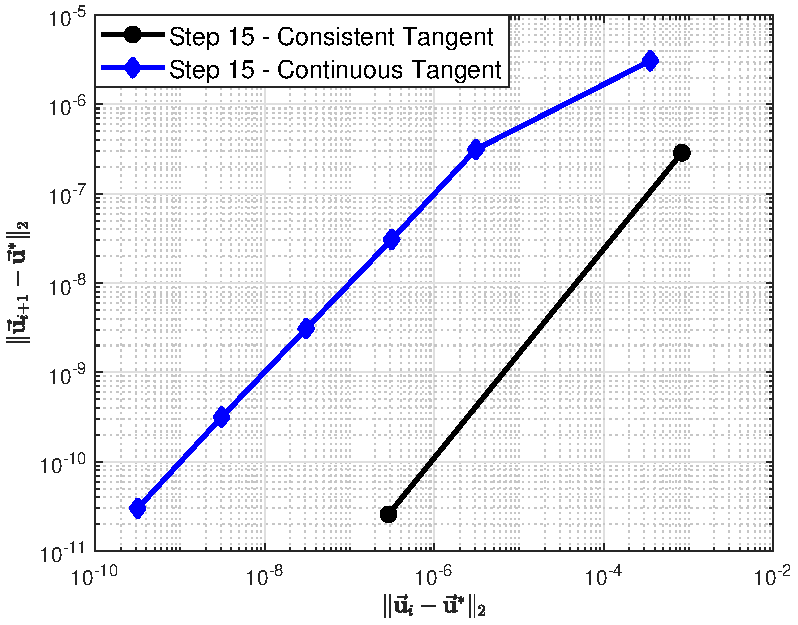
\includegraphics[width=0.45\textwidth]{STEP_15_RATES}%
		\label{fig:STEP15_RATES}%
	}
	\subfloat[Step 25.]{%
		\includegraphics[width=0.45\textwidth]{STEP_25_RATES}%
		\label{fig:STEP25_RATES}%
	}
	\caption{Convergence rates for two representative steps when using the 
		consistent and continuous tangents at fibers.}
	\label{fig:RATES}
\end{figure}

As we reduce the slenderness, slight differences arise compared to a purely 
uniaxial behavior at the fiber. This is mainly due to the assumed strain 
distribution, which is user defined and not accounted in the purely flexural 
model. 


%%%%%%%%%%%%%%%%%%%%  EXAMPLE 5 %%%%%%%%%%%%%%%%%%%%%%%%%%%%%%%%
\subsection{Three Story Frame With Shear Links}

In this example we are concerned with the three-story four-bay steel frame 
shown in Fig. \ref{fig:FIG28_STRUCTURE}. It was first analyzed in 
\cite{Amir2022} and in the present investigation the diagonal braces are 
ignored. 
Gravity loads are 
derived from the material and geometric properties of the elements and, for 
simplicity, are assumed to be acting on frame joints only. The values for each 
joint gravity load are shown in Table \ref{table:TABLE10}. 

\begin{table}[h]
	\centering
	\begin{minipage}{0.7\linewidth}
		\caption{Vertical gravity loads at nodes.}
		\begin{tabular}{cccccccccc}
			\toprule\toprule
			Nodes                         & 2,18 & 3,19 & 4,20& 6,14 & 7,15 & 
			8,16 & 10 & 11 & 12 \\
			\midrule
			$\downarrow P_i \text{(kN)}$  & 240  & 220  & 145 & 340 & 300 & 190 
			& 255 & 215 & 120 \\
			\bottomrule\bottomrule
			\label{table:TABLE10}
		\end{tabular}
	\end{minipage}
\end{table}

A static pushover analysis is then conducted with respect to the 
superimposed horizontal loads on nodes 2,3, 
and 4. All members have 
the same yield stress and Young's modulus: $\sigma_y = 290$ MPa, $E = 210$ GPa, 
and the Poisson's ratio is set to $\nu= 0.3$. Both material and geometric 
nonlinearity options are activated for the 
analysis and perfect plasticity is assumed. 
\begin{figure}[H]
	\centering
	\subfloat[Frame structure.]{%
		\hspace{-0.2cm}\includegraphics[width=0.45\textwidth]{FIG28_STRUCTURE}%
		\label{fig:FIG28_STRUCTURE}%
	}
	\subfloat[Equilibrium paths.]{%
		\includegraphics[width=0.45\textwidth]{FIG28_EQPATHS}%
		\label{fig:FIG28_EQPATHS}%
	}
	\caption{Geometry of the steel frame and \ref{fig:FIG28_EQPATHS} response 
		curves for three different models.}
	\label{fig:FIG28}
\end{figure}

In Fig. \ref{fig:FIG28_EQPATHS} we 
compare the results we get using the hybrid \acrshort{nlp} element with the 
nonlinear flexibility element in 
OpenSees\cite{OpenSees}. In OpenSees we used two different modelling approaches 
with regards to cross-section constitutive behavior: 1) a purely flexural fiber 
section and 2) a section aggregator object, whereby a uniaxial shear 
force-strain law is overloaded on an existing fiber section. In the latter 
approach, the flexural and shear effects remain uncoupled. For the analyses 
using the proposed element, we again adopted 2 different approaches. In the 
first approach we assumed an uncoupled section constitutive law, whereby 
axial-flexural effects are determined by integrating the relevant equations 
over the section fibers while the shear effects are assumed concentrated in the 
centerline. The underlying assumption in this approach is that the shear 
strains are uniform. For the second approach we assumed full coupling at the 
section fibers utilizing the J2 constitutive law and computationally solving 
the stress update problem using the return mapping algorithm proposed in this 
chapter. As can be seen 
from \ref{fig:FIG28_EQPATHS}, the results we get with aggregator sections in 
OpenSees are, expectably, identical with the uncoupled constitutive model when 
using the \acrshort{nlp} element. Both predict a higher  
collapse load than the fully coupled \acrshort{nlp}, which is also an expected 
result. The purely flexural model in OpenSees gives an even slightly higher 
collapse load than the uncoupled models. It is clear that, in the presence of 
shearing components, such as the effective shear wall in this example, a purely 
flexural model will result in non-conservative estimates even in simple 
push-over analyses. 

\begin{figure}[H]
	\centering
	\subfloat[Shear force - centerline shear strain plot.]{%
		\hspace{-0.2cm}\includegraphics[width=0.45\textwidth]{FIG_LINKSHEAR}%
		\label{fig:FIG_LINKSHEAR}%
	}
	\subfloat[Moment - centerline curvature plot.]{%
		\includegraphics[width=0.45\textwidth]{FIG_LINKMOMENT}%
		\label{fig:FIG_LINKMOMENT}%
	}
	\caption{Stress resultant response for the left end of shear link 10-14 for 
		the multiaxial model.}
	\label{fig:FIGLINKS}
\end{figure}



Figures \ref{fig:FIG_LINKSHEAR}, \ref{fig:FIG_LINKMOMENT} highlight the 
differences in the response of shear link 10-14 (left end) when the multiaxial 
constitutive law is used compared to the uncoupled behavior of the section. It 
can be seen that, in addition to higher capacity, the flexural plastification 
for the uncoupled model occurs considerably earlier than the shear one. In 
contrast, the coupled model reaches capacity for both shear and flexural 
response in the same step, which is naturally expected when multiaxial effects 
are considered. These results are derived from the models using the hybrid 
element.

To 
achieve convergent results, the analyses with OpenSees required 90 elements 
with six Gauss-Lobatto points per element for the section aggregator model and 
ten points for the purely flexural model. Each member besides the shear 
links was discretized into 4 nonlinear beam-column elements. In contrast, for 
the analyses using the element proposed in Chapter 2 only one hybrid element 
per 
member was required, resulting in 27 elements in total, and five Gauss-Lobatto 
quadrature points per 
element. Both models account for second order effects under the presence of 
gravity loads.

Lastly, Fig. \ref{fig:COLLAPSE} depicts the progressive plastic hinge formation 
and the eventual collapse mechanism of the frame. Note that the plastic 
mechanism is the same for both the coupled and uncoupled model.

\begin{figure}[H]
	\centering
	\subfloat[Step 30]{%
		\hspace{-0.2cm}\includegraphics[width=0.24\textwidth]{FIG_STEP30}%
		\label{fig:FIG_STEP30}%
	}
	\subfloat[Step 45]{%
		\includegraphics[width=0.24\textwidth]{FIG_STEP45}%
		\label{fig:FIG_STEP45}%
	}
	\subfloat[Step 55]{%
	\includegraphics[width=0.24\textwidth]{FIG_STEP55}%
	\label{fig:FIG_STEP55}%
	}
	\subfloat[Step 68]{%
	\includegraphics[width=0.24\textwidth]{FIG_STEP68}%
	\label{fig:FIG_STEP68}%
	}
	\caption{Progressive collapse of the frame.}
	\label{fig:COLLAPSE}
\end{figure}

%the results we get for 3 
%different modelling 
%options regarding the constitutive law at the fiber level. Both the purely 
%flexural model and the uncoupled elastoplastic model, whereby shear and axial 
%states on fibers are uniaxial and do not interract, yield the same response 
%curve and collapse load. In contrast, the coupled multiaxial model predicts, 
%again, a lower plastic capacity load. 


\section{Summary}

In this chapter a return mapping algorithm for planar, shear 
flexible beam finite elements was presented that fully accounts for 
shear-axial-flexure 
interaction. The proposed formulation is particularly suited for 
flexibility-based or 
hybrid-type elements, which tend to rely more on higher order quadrature rules. 
Focusing our attention on the von Mises yield criterion with both linear 
kinematic and 
isotropic hardening, we have shown that the proposed model is much faster in 
terms of computational cost than 
conventional stress update procedures typically implemented in beam models. In 
addition, we derived the material tangent modulus consistent with the fully 
implicit Euler scheme used for the integration of rate constitutive equations, 
as well as the general form of the consistent section tangent stiffness. It was 
seen that 
the latter depends on the return mapping scheme and the assumption on shear 
strain 
distribution on the cross-section. Use of consistent tangents is crucial in the 
numerical treatment of such problems because they restore the quadratic rates 
of 
converge for the global Newton method. Lastly, the accuracy and efficacy of the 
proposed 
framework was demonstrated in a number of numerical problems, presented in the 
last section. 

%%%%%%%%%%%%%%%%
% Chapter 4
%%%%%%%%%%%%%%%%

\chapter{Discussion}
Lorem ipsum dolor sit amet, consectetur adipiscing elit, sed do eiusmod tempor incididunt ut labore et dolore magna aliqua. Ut enim ad minim veniam, quis nostrud exercitation ullamco laboris nisi ut aliquip ex ea commodo consequat. Duis aute irure dolor in reprehenderit in voluptate velit esse cillum dolore eu fugiat nulla pariatur. Excepteur sint occaecat cupidatat non proident, sunt in culpa qui officia deserunt mollit anim id est laborum..


%%%%%%%%%%%%%%%%
% Chapter 5
%%%%%%%%%%%%%%%%

\chapter{Weighted least squares predictor for numerical continuation}\label{CH5}

%%%%%%%%%%%%%%%%%%%%%%%%%%%%  SECTION 1  %%%%%%%%%%%%%%%%%%%%%%%%%%%
\section{Introduction}\label{CH5-S1}
%%%%%%%%%%%%%%%%%%%%%%%%%%%%%%%%%%%%%%%%%%%%%%%%%%%%%%%%%%%%%%%%%%%%

In this chapter, an efficient prediction 
scheme for numerical continuation of systems of the form $\bvec{F}=\bvec{0}$, 
where $\bvec{F}:\mathbb{R}^{n+1}\rightarrow\mathbb{R}^n$. 
is developed. The formulation does not require second order information, yields 
predictor 
directions consistent with the local geometry of the solution set and remains 
linear in complexity irrespective of the Jacobian structure. It can be 
implemented in any variant of path-tracking algorithms and uses
stabilized local
weighted least squares to fit a local polynomial on the last $k\geq 2$ solution
points, with the weighting function defined so that solution points closer to
the current one are assigned higher weight. This leads to a
versatile scheme where the order of approximation is decoupled from the
points supplanted and can be easily adjusted and updated, if further criteria
are enforced. Moreover, the prediction can be based either on extrapolation 
from the fitted polynomial or its tangent, which is trivial to compute. Since
the solution set of such systems is a curve, the parameterization best suited
for the proposed algorithm is the arc-length of the curve. 

The chapter is structured as follows: in the first section we provide a summary 
numerical continuation. In the second section, the formulation of the Weighted 
Least Squares (\acrshort{wls}) prediction scheme is introduced, followed by a 
section dealing with implementation details. The chapter concludes with a 
section dedicated to numerical tests. We
demonstrate that predictions based on the proposed scheme are competitive
compared to more expensive approaches utilizing the tangent predictor in
terms of total steps, function evaluations and linear solves. Furthermore, it
is shown that they can facilitate the continuation of the tracking process 
even in cases where conventional prediction schemes lead to premature
termination. 


\section{Numerical Continuation}
We focus our attention to undetermined nonlinear systems of the 
form\footnote{In this chapter, we use $\bvec{y}\in\mathbb{R}^{n+1}$ to denote 
any solution vector to an undetermined system $\bvec{F}=\bvec{0}$ and should 
not be confused with the internal field vector $\bvec{y}_i$ introduced in 
Chapter \ref{chapter:CH2}, Sec. \ref{section:CH2-S4}.}:
\begin{equation}
	\bvec{F}(\bvec{y})=0
	\label{eq:Problem}
\end{equation}
where $\bvec{F}:\mathbb{R}^{n+1}\rightarrow\mathbb{R}^n$ is a sufficiently 
smooth
map. Numerical continuation attemps to solve these systems, assuming that the 
regularity assumptions hold. We have already introduced the necessary 
theoretical concepts pertaining to such systems in the previous chapter. In 
what follows, we assume that $\bvec{F}$ is a sufficiently smooth map and 
$\bvec{0}$ is a regular value for system (\ref{eq:Problem}. Under these 
assumptions, the solution set
$\mathcal{S}$ is a one-dimensional manifold in
$\mathbb{R}^{n+1}$ consisting of connected components homeomorphic to the real
line (paths) and the unit circle (loops) and with the same smoothness as
$\bvec{F}$. For $\mathcal{S}$ we have:
\begin{equation}
	\mathcal{S}=\{\bvec{y}\in\mathbb{R}^{n+1}\ |\ 
	\bvec{F}(\bvec{y})=\bvec{0}\},\quad \text{and}\quad 
	\text{rank}(\bmat{J})=n\ \forall\bvec{y}\in\mathcal{S}
	\label{eq:SolutionSet}
\end{equation}

\noindent where $\bmat{J}$ is the Jacobian of $\bvec{F}$. Then,  by the 
implicit
function theorem there exists 
$\bvec{\phi}(s):\mathbb{R}\rightarrow\mathbb{R}^{n+1}$
such that $\bvec{F}(\bvec{\phi}(s))=\bvec{0}$. In other words, paths or loops in
$\mathcal{S}$ implicitly defined by \ref{eq:Problem} can be parameterized with
respect to $s$ and, thus, $\bvec{y}(s)\equiv\bvec{\phi}(s)$. Differentiating 
\ref{eq:Problem} with respect to $s$, we arrive
at the following Initial Value Problem (\acrshort{ivp}):
\begin{subequations}
	\begin{align}
		&\bmat{J}(\bvec{y})\dot{\bvec{y}}=0\label{eq:IVP1}\\
		&\bvec{y}(0)=\bvec{y}_0,\quad \bvec{F}(\bvec{y}_0)=\bvec{0}	
		\label{eq:IVP2}
	\end{align}
	\label{eq:IVP}
\end{subequations}
\begin{figure}[t]
	\centering
	\includegraphics[scale=1.0]{FIG41.pdf}
	\caption{Advancing from step $N$ to step $N+1$ using a PC approach.}
	\label{fig:FIG41}
\end{figure}
where $\dot{(\cdot)}$ denotes differentiation with respect to $s$ and 
$\dot{\bvec{y}}$ is the tangent vector to the solution curve at $\bvec{y}(s)$. 

The implicit function theorem forms the basis of numerical
continuation\cite{Allgower:2003,Rheinboldt75,Rheinboldt:2000,Rheinboldt:1980,
Garcia:1980,Watson86,Keller:1978}, which aim to track solution sets in 
$\mathcal{S}$. The idea is to generate a sequence of points
$\{\bvec{y}_1,\bvec{y}_2,\cdots,\}$, with 
$\bvec{F}(\bvec{y}_i)\approx\bvec{0}$  by solving
\ref{eq:IVP} in a step-by-step fashion using a Predictor-Corrector 
(\acrshort{pc}) scheme. The orientation of tracking is chosen by assigning a 
sign to the tangent vector and the positive orientation is
characterized by condition $\text{det}(\bigl[
\begin{smallmatrix}
	\bmat{J} \\ \dot{\bvec{y}}
\end{smallmatrix}
\bigr]) > 0$. If $s$ is assumed to be the arc-length of the solution curve, then
$\dot{\bvec{y}}(s)$ is a unit tangent vector and \ref{eq:IVP} is supplemented by
condition $\left\Vert \dot{\bvec{y}}(s)\right\Vert_2=1$, where $\left\Vert
\cdot\right\Vert_2$ denotes the Euclidian norm.

Different initial points $\bvec{y}_0$ might
lead to a different path(loop) to be tracked and each point generated by 
\acrshort{pc} methods is considered to be in the proximity of the solution 
curve. As shown in \ref{fig:FIG41}, to advance from the
current step $N$\footnote{The use of $N$ to designate the step counter in this 
chapter should not be confused with the same symbol used in Chapter 
\ref{chapter:CH2} to represent the axial stress resultant in a cross-section.} 
with known solution $\bvec{y}_N$ to step $N+1$, a
prediction for $\bvec{y}_{N+1}$ is first made, $\bvec{y}_{N+1}^p$, followed by 
a 
correction phase 
whereby the initial prediction is iteratively improved, usually by employing a
Newton type iteration to enforce condition \ref{eq:Problem}. Satisfaction of
this condition is usually tested using an appropriate norm and a
prescribed tolerance. 

Assuming that the path is parameterized by $s$ so that
$\bvec{y}=\bvec{y}(s)$, these two phases can be succintly stated as follows:
\begin{enumerate}[noitemsep]
	\item Prediction: $\bvec{y}^p_{N+1}=\bvec{G}(s_N+\Delta s)$
	\item Correction: $\bvec{y}^{j+1}_{N+1} = 
	\bvec{y}^j_{N+1}+\bmat{B}^j\bvec{F}(\bvec{x}^j_{N+1})$, $j=0,1,\cdots
	j_{max}$, $\bvec{y}^0_{N+1}=\bvec{y}^p_{N+1}$
\end{enumerate}
Both $\bvec{G}$ and $\bmat{B}$ depend on the predictor and corrector algorithms 
used. For
example, if the Euler predictor is used, then $\bvec{G}=\bvec{y}(s)$ and 
$\bvec{G}(s_N+\Delta
s)\approx \bvec{y}_N+\Delta s \dot{\bvec{y}}_N$ around $\bvec{y}_N$. In 
addition, if $\bmat{B} = \bmat{J}^T(\bmat{J}\bmat{J}^T)^{-1}$, then the
correction phase arrives at the least squares solution for $\bvec{y}_{N+1}$, 
with $\bmat{B}$ being the Moore-Penrose inverse of $\bmat{J}$. 
In general, the determining characteristics for a \acrshort{pc} algorithm are:
\begin{itemize}[noitemsep]
	\item Choice of parameterization 
	\item Type of predictor
	\item Type of corrector
	\item Determination and control of step-length $\Delta s$
\end{itemize}
While the most computationally costly part in \acrshort{pc} methods is the 
correction phase, efficient step-length adjustment schemes in conjunction with 
fast and reliable prediction phases can also
contribute significantly to the performance of the \acrshort{pc} algorithm.

Predictors can be categorized in three families:
\begin{enumerate}[noitemsep]
	\item Predictors based on functional extrapolation
	\item Predictors based on derivative information of $\bvec{F}$
	\item A combination of 1 and 2
\end{enumerate}
As an example of type 1 prediction, a Lagrange interpolating polynomial, $L(s)$,
can be used to extrapolate from a set of the $k$ most recent solution points 
$\{\bvec{y}_{N-k+1},\cdots,\bvec{y}_N\}$ such that 
$\bvec{y}^p_{N+1}=L(s_N+\Delta
s)$\cite{Rheinboldt75,Deuflhard87}. The
Euler predictor using the tangent $\dot{\bvec{y}}_N$ as a direction is the 
simplest
case of the second type. Finally, a case of type 3 predictors are those derived 
from interpolations that utilize derivative information, such as the Hermite 
interpolating polynomials. In \ref{fig:FIG42} the two generic cases of 
predictors are illustrated.

\begin{figure*}[t]
	\centering
	\subfloat[][]{{\includegraphics[width=6.1cm]{FIG42_INTERP.pdf}}\label{FIG42_INTERP}}%
	\qquad
	\subfloat[][]{{\includegraphics[width=6.1cm]{FIG42_TANGENT.pdf}}\label{FIG42_TANGENT}}%
	\caption{Two types of predictors: (a) interpolatory and (b) Euler
		predictor.}%
	\label{fig:FIG42}%
\end{figure*}

In general, predictors based on extrapolation of an
interpolating function tend to be sensitive to variations in accuracy of the 
computed set
$\{\bvec{y}_i\}_{i=1}^N$ and although they are computationally inexpensive, the 
quality of prediction worsens as the 
step-length becomes
larger. For that reason, predictors of order higher than two are rarely
used\cite{Seydel87,Salgovic81}. On the other side, type 2 or 3
predictors\cite{Schwetlick87,Gervais04,Syam02,Syam03,Watson87,Deuflhard87,Lundberg93},
 tend to yield better approximations for larger step-lengths but are 
considerably more computationally expensive. Tangent vectors need to be
extracted from the nullspace of $\bmat{J}$ at the beginning of each step and
the determination of higher order derivatives require additional linear systems
to be solved. Alternatively, finite difference schemes can be employed to
approximate higher order quantities, but these too require additional functional
evaluations. An alternative way to categorize predictors is based on whether
they rely solely on information at $\bvec{y}_N$ or incorporate previous steps as
well\cite{Allgower91}. Since the predictor developed in this chapter is by 
construction a multistep formulation, the categorization
presented here will help highlight type 1 and type 2 predictor variants that
arise from the propsed \acrshort{wls} scheme.



%%%%%%%%%%%%%%%%%%%%%%%%%%%%  SECTION 2  %%%%%%%%%%%%%%%%%%%%%%%%%%%
\section{Weighted Least Squares Predictor}\label{CH5-S2}
%%%%%%%%%%%%%%%%%%%%%%%%%%%%%%%%%%%%%%%%%%%%%%%%%%%%%%%%%%%%%%%%%%%%

In this section we formulate the Weighted Least Squares (\acrshort{wls}) 
predictor. Let $k$, $m\in\mathbb{Z}^+$, $k>m$, be parameters that designate the 
last $k$ 
steps, including the current step, $N$, and the degree of polynomial space,
$\mathcal{P}_m(\mathbb{R}_{\geq0},\mathbb{R})$,
respectively.
We assume convergence has been achieved at step $N$ and all
relevant quantities for the last $k$ steps are known. 
 For ease of notation, we restrict our presentation to a particular
component of $\bvec{y}=[ y_1\ \cdots\ y_l\ \cdots\  y_{n+1}]^T$, $y_l$, and 
omit 
the index from derivations.  Therefore, in what follows, quantities
$y_N$, $y_{N-1}\mathbb{R}$
are to be understood as the $l$-th components of $\bvec{y}\in\mathbb{R}^{n+1}$ 
at steps $N$ and $N-1$ respectively unless explicitly stated otherwise. 

Let $\bar{y}(s)\in\mathcal{P}_m$ be the fitted polynomial at the last $k$ points
$\set{y_i}_{i=N-k+1}^N$ using a \acrshort{wls} approach, where $y_i=y(s_i)$, 
such that:
\begin{equation}
	\bar{y}(s) = b_0+b_1s+\cdots +b_ms^m=\bvec{p}^T\bvec{b}
	\label{eq:FIT}
\end{equation}
where $\bvec{p}=[1\ s\ \dots\ s^m]^T$ and $\bvec{b}=[b_0\ b_1\ \dots\ b_m]^T$ 
are the polynomial basis and coefficient vectors respectively. 
The ``energy" function associated with the \acrshort{wls} fitting in this case 
is:
\begin{equation}
	J = \sum_{\substack{j=\\ N-k+1}}^N w(s_j)\bigg[\bar{y}(s_j)-y_j\bigg]^2
	\label{eq:LeastSquarefun}
\end{equation}
where $w(s)$ is the weight function, unspecified for now. Minimization of $J$ 
with respect to $\bvec{b}$ yields the so-called normal equations for the least
squares solution: 
\begin{equation}
	\bmat{A}\bvec{b}=\bvec{f}
	\label{eq:NORMAL}
\end{equation}
with \ref{eq:FIT} substituted in \ref{eq:LeastSquarefun}. The moment
matrix $\bmat{A}$ and ``force" vector $\bvec{f}$ are given by:
\begin{subequations}
	\begin{align}
		\bmat{A} &= \sum_{\substack{j=\\ N-k+1}}^N 
		w_j\bvec{p}(s_j)\bvec{p}(s_j)^T\label{eq:moment}\\ 
		\bvec{f} &= \sum_{\substack{j=\\ N-k+1}}^N 
		w_jy_j\bvec{p}(s_j)\label{eq:force}
	\end{align}
	\label{eq:MOMENTEQS}
\end{subequations}
Since the path is
parameterized by the arc-length $s$, which is taken here as the independent
parameter of the \acrshort{wls} fitting, a stabilization measure is required 
for the case
that $s$ becomes excessively large. In such a scenario, the moment matrix
$\bmat{A}$ becomes ill-conditioned. To deal with this issue, we transform the 
polynomial basis and work instead in $\mathcal{P}_m([-1,1],\mathbb{R})$. 
That is:
\begin{equation}
	\bar{y}(s) = \bvec{c}^T\bvec{\rho}
	\label{eq:TFIT}
\end{equation}
where now $\bvec{\rho}=[\rho_0\ \rho_1\ \dots\ \rho_m]$ is the coefficient 
vector for the
transformed basis and $\bvec{c}$ is:
\begin{equation}
	\bvec{c} = \begin{bmatrix}
		1 & \dfrac{s-s_r}{h} & (\dfrac{s-s_r}{h})\strut^2 & \dots &
		(\dfrac{s-s_r}{h})\strut^m
	\end{bmatrix}^T
	\label{eq:TPOLYBASIS}
\end{equation}
with $s_r=(s_N+s_{N-k+1})^{}/2$, $h=(s_N-s_{N-k+1})^{}/2$ and $s\in[s_{N-k+1},\
s_N]$. The transformation between the basis vectors $\bvec{p}$ and $\bvec{c}$ is
carried out by operator $\bmat{\Phi}$:
\begin{equation}
	\bvec{c}=\bmat{\Phi}\bvec{p}
	\label{eq:Transf}
\end{equation}
where
\begin{equation}
	\bmat{\Phi} = \begin{bmatrix}
		1        &      0      & \dots & 0 & 0\\
		-\frac{s_r}{h} & \frac{1}{h} & \dots & 0 & 0\\
		\vdots     & \vdots      & \ddots& 0 & 0\\
		\frac{(-s_r)^m}{h^m} & \binom{m}{m-1}\frac{(-s_r)^{m-1}}{h^m} & \dots
		& -\binom{m}{1}\frac{s_r}{h^m} & \frac{1}{h^m}
	\end{bmatrix}
	\label{eq:OPERATOR}
\end{equation}
Similarly, for the coefficient vectors we have:
\begin{equation}
	\bvec{b}=\bmat{\Phi}^T\bvec{\rho}
	\label{eq:QoeffTransf}
\end{equation}
Using \ref{eq:TFIT} and $\bvec{p}=\bmat{\Phi}^{-1}\bvec{c}$ from 
\ref{eq:Transf}, 
the
normal equations in the trasnformed basis are:
\begin{equation}
	\bmat{A}_c\bvec{\rho}=\bvec{f}_c
	\label{eq:TNORMALS}
\end{equation}
where $\bmat{A}_c$, $\bvec{f}_c$ are determined from \ref{eq:MOMENTEQS} with
$\bvec{p}(s_j)\rightarrow \bvec{c}(s_j)$. Using 
\ref{eq:FIT},\ref{eq:QoeffTransf},
and that $\bvec{\rho}=\bmat{A}^{-1}\bvec{f}_c$ from \ref{eq:TNORMALS}, the 
stabilized weighted least squares fit for component $y$ in the original
space is given by:
\begin{equation}
	\bar{y}(s)=\bvec{p}(s)^T\bvec{b}
	\label{eq:SWLSF}
\end{equation}
where
\begin{equation}
	\bvec{b} = \bmat{\Phi}^T\bmat{A}_c^{-1}\bvec{f}_c
	\label{eq:compCoef}
\end{equation}
Notice that $\bmat{A}_c$ is common for all components $y_l,\ l=1,\dots, n+1$ in
$\bvec{y}$ and only the forcing the ``force" vector $\bvec{f}_c$ has to be
evaluated for each component. That is, only the coefficient vector is component
dependent: $\bvec{b}\rightarrow \bvec{b}(y_{N-k+1},...,y_N)$. 

%%%%%%%%%%%%%%%%%%%%%%%%%% SECTION 2 - SUBSECTION 1 %%%%%%%%%%%%%%%%%%%%%%%%%%%
\subsection{Matrix Formulation of WLS Approximation}\label{CH5-S2SS1}

We now
derive the matrix relations of the \acrshort{wls} process, which incorporate 
all 
components. This can be represented succintly by collecting all the involved 
quantities corresponding to differnet components of $\bvec{y}$ into matrices. 
The local approximation to solution curve $\bvec{y}(s)$ is as follows:
\begin{equation*}
	\bvec{y}\approx \bar{\bm{y}}(s)=\begin{bmatrix}
		\bar{y}_1(s)\\ \bar{y}_2(s)\\ \vdots \\ \bar{y}_{n+1}(s)
	\end{bmatrix}
\end{equation*}
which holds for $s\in[s_{N-k+1},\ s_N]$ and all solution points 
corresponding to that interval\footnote{Note that $\bar{\bm{y}}(s)$ is a 
vector. 
It denotes an approximation to vector $\bvec{y}$. The overhead arrow is omitted 
in order to avoid excessive use of notation.}. Let $\bmat{P}$ be defined as 
follows:
\begin{equation}
	\bmat{P}=\begin{bmatrix}
		\bvec{p}(s_{N-k+1}) & \dots & \bvec{p}(s_N)
	\end{bmatrix}=\begin{bmatrix}
		1 &  \dots & 1\\
		s_{N-k+1} & \dots & s_N\\
		\vdots & \ddots & \vdots\\
		s_{N-k+1}^m & \dots & s_N^m
	\end{bmatrix}
	\label{eq:P}
\end{equation}
with its counterpart  in the transformed basis given by
\begin{equation}
	\bm{\mathcal{C}}=\bmat{\Phi}\bmat{P}
	\label{eq:TransMat}
\end{equation}
where $\bm{\mathcal{C}}$ is defined in accordance with $\bmat{P}$: 
$\bm{\mathcal{C}}= 
\begin{bmatrix}
	\bvec{c}(s_{N-k+1}) & ... & \bvec{c}(s_N)
\end{bmatrix}$. We also define $\bmat{W}=\text{diag}(w_{N-k+1},\dots,w_N)$. From
\ref{eq:SWLSF}, \ref{eq:force} and \ref{eq:Transf}, the coefficient vector
for component $l$ in $\bar{\bvec{y}}$, $\bvec{b}_l$, 
can be expressed in the 
following way:
\begin{equation}
	\bvec{b}_l = 
	\bmat{\Phi}^T\bmat{A}_c^{-1}\bm{\mathcal{C}}\bmat{W}\begin{bmatrix}
		y_{N-k+1,l} \\ y_{N-k+2,l}\\ \vdots \\ y_{N,l}
	\end{bmatrix}_{(k\times 1)}
	\label{eq:coeff2}
\end{equation}
By extension, a concise expression for $\bar{\bvec{y}}$, whose component form is
\ref{eq:SWLSF}, is then:
\begin{equation}
	\bar{\bm{y}}=\bvec{p}(s)^T\bm{\mathcal{B}}
	\label{eq:globalSWLSF}
\end{equation}
where
\begin{equation}
	\bm{\mathcal{B}}=\bmat{\Phi}^T\bmat{A}_c^{-1}\bm{\mathcal{C}}\bmat{W}\bmat{Y}
	\label{eq:B}
\end{equation}
and $\bmat{Y}$ is a $k\times(n+1)$ matrix whose $l$-th column contains
the values of the $l$-th component of $\bvec{y}$ at the last $k$ points
supplied to the algorithm (see Eq. (\ref{eq:coeff2})):
\begin{equation}
	\bmat{Y}=\begin{bmatrix}
		y_{N-k+1,1} & y_{N-k+1,2} & \dots & y_{N-k+1,n+1}\\
		y_{N-k+2,1} & y_{N-k+2,2} & \dots & y_{N-k+2,n+1}\\
		\vdots      & \vdots      & \ddots & \vdots\\
		y_{N,1} & y_{N,2} & \dots & y_{N,n+1}\\
	\end{bmatrix}
	\label{eq:Y}
\end{equation}
We observe from \ref{eq:globalSWLSF} (or \ref{eq:SWLSF}) that derivatives up 
to order $m$ can be computed directly by simple differentiation of the 
polynomial basis vector $\bvec{p}(s)$:
\begin{align}
	& \text{Component form} && \text{Vector form}\nonumber\\
	&\dot{y} = \dot{\bvec{p}}(s)^T\bvec{b}\ , &&
	\dot{\bar{\bm{y}}}= \dot{\bvec{p}}(s)^T\bm{\mathcal{B}}\nonumber\\
	&\ddot{y} = \ddot{\bvec{p}}(s)^T\bm{b}\ , &&
	\ddot{\bar{\bm{y}}}= \ddot{\bvec{p}}(s)^T\bm{\mathcal{B}}\nonumber\\
	&\vdots && \vdots\nonumber
\end{align}
with 
\begin{align*}
	&\dot{\bvec{p}}(s)=\begin{bmatrix}
		0 & 1 & 2s & \dots & ms^{m-1}
	\end{bmatrix}\\
	&\ddot{\bvec{p}}(s)=\begin{bmatrix}
		0 & 0 & 2 & \dots & m(m-1)s^{m-2}
	\end{bmatrix}\\
	&\vdots
\end{align*}


%%%%%%%%%%%%%%%%%%%%%%%%%% SECTION 2 - SUBSECTION 2 %%%%%%%%%%%%%%%%%%%%%%%%%%%
\subsection{WLS Prediction Variants}\label{CH5-S2SS2}

Given an increment in the arc-length $\Delta s$, a straightforward prediction
scheme is given by extrapolating from the fitted curve, $\bar{\bvec{y}}$ at 
$s_N$:
\begin{equation}
	\bvec{y}^p = \bar{\bvec{y}}(s_N+\widetilde{\Delta s})
	\label{eq:WLSE}
\end{equation}
where $\widetilde{\Delta s}$ is introduced to account for the fact that $s$ is
not actually the arc-length of the solution curve $\bvec{y}(s)$ and use of 
$\Delta s$ can 
sometimes lead to unpredicable behavior. A stabilization procedure for is 
presented in the next part of this section. 

We will refer to prediction (\ref{eq:WLSE}) as Weighted Least Squares 
Extrapolation (\acrshort{wlse}) predictor. A second approach is to derive the 
prediction direction from first order
information of the local \acrshort{wls} curve, which is trivial to retrieve. We 
propose the following general formula:
\begin{equation}
	\bvec{y}^p = \bvec{y}_N + \Delta s\ \bvec{t}_z
	\label{eq:WLSIT}
\end{equation}
where $\bvec{t}_z$ is a unit vector determined as follows:
\begin{equation}
	\bvec{t}_z = \dfrac{\dot{\bar{\bm{y}}}(s_N+z\widetilde{\Delta
			s})}{\Vert\dot{\bar{\bm{y}}}(s_N+z\widetilde{\Delta s})\Vert_2}
	\label{eq:ImplicitTangent}
\end{equation}
with $\dot{\bar{\bm{y}}}(s)=\dot{\bvec{p}}(s)^T\bm{\mathcal{B}}$ and $z\in[0\ 
1]$. For
$z\neq 0$, the direction is derived by extracting the tangent of the fitted
curve ahead of the current solution point, whereas for $z=0$ the normalized 
tangent of $\bar{\bm{y}}(s_N)$ is used instead and this yields a
\acrshort{wls} approximation to the standard Euler predictor. Normalization is 
required
because the $\dot{\bar{\bm{y}}}$ is not a unit vector. When $z>0$, will refer to
this prediction scheme as the Weighted Least Squares Implicit Tangent 
(\acrshort{wlsit}) predictor. In the case that $z=0$, we term it Weighted Least 
Squares Tangent
(\acrshort{wlst}) predictor. Notice that, in any case, \acrshort{wlsit} 
involves extrapolation and,
therefore, the steplength adjustment procedure for $\widetilde{\Delta s}$ is
required here as well. For illustrative purposes, the predictors 
\acrshort{wlse}, \acrshort{wlst}
and \acrshort{wlsit} with $z=1$ are depicted in 
\ref{fig:DifferentialPredictors}.
\begin{figure}[t]
	\centering
	\includegraphics[scale=1.]{FIG43.pdf}
	\caption{Geometric interpretation of predictors (i)WLSE (blue), (ii) WLSIT
		(light blue, $z=1$), and (iii) WLST (red, $z=0$).}
	\label{fig:DifferentialPredictors}
\end{figure}

%%%%%%%%%%%%%%%%%%%%%%%%%% SECTION 2 - SUBSECTION 3 %%%%%%%%%%%%%%%%%%%%%%%%%%%
\subsection{Arc-length Stabilization}\label{CH5-S2SS3}

Given a step-length $\Delta s$, the \acrshort{wlse} predictor estimates the 
next solution point using \ref{eq:WLSE}. To determine $\widetilde{\Delta s}$ 
given $\Delta s$,we impose condition
\ref{eq:Constraint}:
\begin{equation}
	\Vert \bvec{y}^p-\bvec{y}_N\Vert_2^2-\Delta s^2 = 0
	\label{eq:Constraint}
\end{equation}
where in place of $\bvec{y}^p$ (see \ref{eq:WLSE}) we use its first order 
approximation:
\begin{equation}
	\bvec{y}^p\approx 
	\bar{\bm{y}}(s_N)+\dot{\bar{\bm{y}}}(s_N)\widetilde{\Delta s}
	\label{eq:1stOrder}
\end{equation}
Let $\bvec{y}_0=\bvec{y}_N$, $\bar{\bm{y}}_0 = \bar{\bm{y}}(s_N) =
\bvec{p}(s_N)^T\bm{\mathcal{B}}$ and $\dot{\bar{\bm{y}}}_0 = 
\dot{\bar{\bm{y}}}(s_N) = \dot{\bm{p}}(s_N)^T\bm{\mathcal{B}}$. Then,
substituting \ref{eq:1stOrder} into \ref{eq:Constraint} yields the following
quadratic equation to be solved for $\widetilde{\Delta s}$:
\begin{equation}
	\Vert\dot{\bar{\bm{y}}}_0\Vert_2^2(\widetilde{\Delta s})^2+
	2(\bar{\bm{y}}_0-\bm{y}_0)^T\dot{\bar{\bm{y}}}_0 \widetilde{\Delta s}+
	\Vert \bar{\bm{y}}_0-\bm{y}_0\Vert_2^2-\Delta s^2=0
	\label{eq:QUADRATIC_STAB}
\end{equation}
This leads to two roots, of which the smallest positive one is chosen:
\begin{equation}
	\widetilde{\Delta s}_{1,2} =
	\dfrac{-2(\bar{\bm{y}}_0-\bm{y}_0)^T\dot{\bar{\bm{y}}}_0\pm\sqrt{\Delta}}
	{2\Vert\dot{\bar{\bm{y}}}_0\Vert_2^2}
	\label{eq:ROOTS}
\end{equation}
where the discriminant is $\Delta = 4\Vert
\bar{\bm{y}}_0-\bm{y}_0\Vert^2_{\bmat{N}} -
4\Vert\dot{\bar{\bm{y}}}_0\Vert_2^2(\Vert
\bar{\bm{y}}_0-\bm{y}_0\Vert_2^2-\Delta s^2)$, with $\bmat{N} = 
\dot{\bar{\bm{y}}}_0\dot{\bar{\bm{y}}}_0^T$. Condition $\Delta > 0$ leads to
the following requirement for the user-defined step-length $\Delta s$ if the
\acrshort{wlse} predictor is used:
\begin{equation}
	\Delta s > \sqrt{\Vert \bar{\bm{y}}_0-\bm{y}_0\Vert_2^2-
		\dfrac{\Vert 
		\bar{\bm{y}}_0-\bm{y}_0\Vert^2_{\bmat{N}}}{\Vert\dot{\bar{\bm{y}}}_0
			\Vert_2^2}}
	\label{eq:DSREQ}
\end{equation}

%%%%%%%%%%%%%%%%%%%%%%%%%% SECTION 2 - SUBSECTION 4 %%%%%%%%%%%%%%%%%%%%%%%%%%%
\subsection{The Weight Function}\label{CH5-S2SS4}

We now discuss the weighting function $w(s)$. The reasoning for introducing a
weighting in the least squares fitting is as follows: since with
the ``exact" tangent predictor the direction is determined by the neighborhood 
of
the current solution $\bvec{y}_N$ in the differential sense, we need to assign
different weights to the precceding $k-1$ solution points we provide for the 
least squares fitting. A reasonable option for $w(s)$, which is depicted in 
Fig. \ref{fig:44}, is a generalization of the unit ramp function:
\begin{align}
	&w(s) = \alpha + \frac{s-s_{N-k+1}}{s_N-s_{N-k+1}}(1-\alpha)
	\label{eq:WeightFunction},\quad \alpha\in[0\ 1]
\end{align}
By choosing $\alpha=0$, the unit ramp function is obtained, while for
$\alpha=1$, all solution points are assigned unit weight, $w(s)=1$, with 
$s\in[s_{N-k+1}\ s_N]$.
With this weighting plan, it is
ensured points closer to the current solution are assigned higher importance,
with $\bvec{y}_N$ having the highest weight by construction. If the unit ramp is
used, it is crucial that the implementation ensures there are enough points for
the least squares algorithm to commence. This is because the point that
corresponds to step $N-k+1$ is now assigned a zero weight and, thus, it doesn't
contribute in the moment matrices $\bmat{A},\ \bmat{A}_c$(see Eqs.
(\ref{eq:LeastSquarefun}),(\ref{eq:moment})). This issue arises when the mimimum
points for the desired degree of approximation are supplied. 

\begin{figure}[t]
	\centering
	\includegraphics[scale=1]{FIG44.pdf}
	\caption{Weight function $w(s)$ of the WLS predictor.}
	\label{fig:FIG44}
\end{figure}


%%%%%%%%%%%%%%%%%%%%%%%%%%%%  SECTION 3  %%%%%%%%%%%%%%%%%%%%%%%%%%%
\section{Implementation}\label{CH5-S3}
%%%%%%%%%%%%%%%%%%%%%%%%%%%%%%%%%%%%%%%%%%%%%%%%%%%%%%%%%%%%%%%%%%%%

%%%%%%%%%%%%%%%%%%%%%%%%% SECTION 3 - SUBSECTION 1  %%%%%%%%%%%%%%%%%%%%%%%%%%%
\subsection{Algorithm}\label{CH5-S3SS1}
We outline the basic steps in the implementation of the \acrshort{wls}
predictor in pseudocode format. We assume all quantities at the current step
$N$ are known.

\begin{algorithm}[t]
	\caption{Weighted Least Squares Predictor pseudocode}
	\label{alg:WLS}
	\begin{algorithmic}
		\STATE{\textbf{Input}: $m$, $k$, $\set{y_i}_{i=N-k+1}^N$,
			$\set{s_i}_{i=N-k+1}^N$, $\Delta s$, $\alpha$, $z$}
		\STATE{Determine $\bmat{\Phi}$, $\bmat{Y}$ and initialize $\bmat{A}_c$,
			$\bmat{W}$, $\bm{\mathcal{C}}$}
		\FOR{$i =k,k-1\dots,1$}
		\STATE{$s_i\gets s_{N-i+1}$ }
		\STATE{Get shifted basis at $s_i$, $\bvec{c}(s_i)$, and add to $i$-th 
		column in
			$\bm{\mathcal{C}}$}
		\STATE{Determine weight, $w_i$, and add it to component $(i,i)$ in 
		$\bmat{W}$}
		\STATE{$\bmat{A}_c\gets \bmat{A}_c+w_j\bvec{c}(s_i)\bvec{c}(s_i)^T$}
		\ENDFOR
		\STATE{$\bm{\mathcal{B}}\gets 
		\bmat{\Phi}^T\bmat{A}_c^{-1}\bm{\mathcal{C}}\bmat{W}\bmat{Y}$} 
		\STATE{Determine $\widetilde{\Delta s}$\hspace{4cm}// 
		\textit{Step-length
				stabilization}}
		\STATE{}
		\STATE{// \textit{WLSE}}
		\STATE{$s\gets s_N+\widetilde{\Delta s}$}
		\STATE{Get polynomial basis at $s$, $\bm{p}(s)$}
		\STATE{$\bvec{y}^p_{N+1}\gets \bvec{p}(s)^T\bm{\mathcal{B}}$}
		\STATE{}
		\STATE{// \textit{WLSIT}}
		\STATE{$s\gets s_N+z\widetilde{\Delta s}$}
		\STATE{Get first derivative of polynomial basis at $s$, 
		$\dot{\bvec{p}}(s)$}
		\STATE{$\bvec{v}\gets \dot{\bvec{p}}(s)^T\bm{\mathcal{B}}$}
		\STATE{$\bvec{t}_z\gets \bvec{v}^{}/\Vert\bvec{v}\Vert_2$}
		\STATE{$\bvec{y}^p_{N+1}\gets \bvec{y}_N + \Delta s\bvec{t}_z$}
		\STATE{}
		\RETURN $\bvec{y}^p_{N+1}$
	\end{algorithmic}
\end{algorithm}

As can be seen from \ref{alg:WLS}, the \acrshort{wls} process requires the 
polynomial degree  $m$ we use for the fitting, the number of solution 
points $k$ we take into account starting from the current one at step $N$, 
along with the curve lengths at those points. We also need to specify values for
parameter $\alpha$ (see \ref{eq:WeightFunction}) and $z$, in case the 
\acrshort{wlsit}
predictor is selected. Finally, a step-length, $\Delta s$, also needs to be
provided. The most expensive action is the computation of the coefficient matrix
$\bm{\mathcal{B}}$. More specifically, the number of floating point operations 
is
commensurate to the term $2(m+1)k(n+1)$ or, simply, $2(m+1)kn$, where $n$ is
the size of $\bvec{y}$ after ignoring one component. In other words, it
is of $\mathcal{O}(n)$ (time) complexity. Coupled with a degree control check, 
whereby
$m$ can be adjusted based on local properties of the path tracked so far, we 
expect high values for the coefficient only in highly nonlinear regions. 

\subsection{Arc-Length Measurement}
Prediction schemes that rely on some form of extrapolation require measurement 
of the current curve length, $s$, as the solution 
process progresses. The most direct and easy way
to compute the curve length at discrete points is by summation of lengths  
of the line segments connecting them. After convergence is achieved at step $N$,
the length of the segment between $\bvec{y}_{N-1}$ and $\bvec{y}_N$ is 
approximated as follows:
\begin{equation}
	s_N=s_{N-1}+Ds
	\label{eq:newS}
\end{equation}
where
\begin{equation}
	Ds = \Vert \bvec{y}_N-\bvec{y}_{N-1}\Vert_2
	\label{eq:SegmentLength}
\end{equation}
If \ref{eq:Problem} is the finite-dimensional approximation of some operator
equation, then it is recommended\cite{Keller87} that we account for the fact
that, as is customary, the first $n$ components are members of some function
space (e.g. a Banach space) and, therefore, \ref{eq:SegmentLength} should in 
some sense approximate the underlying $L^2$ norm:

\begin{equation}
	Ds = \Vert 
	\bvec{y}_N-\bvec{y}_{N-1}\Vert_{L^2}=\sqrt{h_m^d\sum_{i=1}^n(y_{i,N}-y_{i,N-1})^2+(y_{n+1,N}-y_{n+1,N-1})^2}
	\label{eq:INCR}
\end{equation}
where the $n+1$ component in $\bvec{y}$ is considered as an additional 
parameter and
$h_m$,$d$ are the mesh spacing and the spatial dimension of the problem 
respectively.


%%%%%%%%%%%%%%%%%%%%%%%%% SECTION 3 - SUBSECTION 2  %%%%%%%%%%%%%%%%%%%%%%%%%%%
\subsection{Discussion}\label{CH5-S3SS2}

It is clear that, in general,  
$\bar{\bm{y}}(s_j)\neq \bvec{y}_j$ for $j=N-k+1,\dots, N$, which is 
expected since this is not, necessarily,
an interpolatory approximation. The interpolatory
condition can be retained if the relation between the number of solution
points supplied, $k$, and the degree of the polynomial space, $m$, is $k=m+1$.
Furthermore, the degree of approximation
is uncoupled from the number of points supplied, while in conventional 
interpolatory
schemes this is not the case. We suspect this is one of the reasons some
researchers claim higher order predictors based on extrapolation generally 
behave poorer than the secant 
predictor\cite{Seydel87,Salgovic81}. In addition, the \acrshort{wls} predictor 
does
not rely on derivative information of $\bvec{F}$ and, therefore, its 
performance in
terms of computational cost is independent of the structure of the Jacobian.
This is particularly important for problems without properties like sparsity or
bandedness to exploit numerically. For the \acrshort{wlsit} variant, we instead 
use the local \acrshort{wls} approximation to extract derivatives
when and if necessary. For step-length, $\Delta s$, of reasonable magnitude, 
the local \acrshort{wls}
fitting is able to give a better approximation of the local geometry, especially
closer to sudden changes in curvature of the solution curve. This is precisely
due to the fact that interpolation is not enforced. Furthermore, since
extraction of the actual tangent vector from the nullspace of the Jacobian is 
not required, \acrshort{wls} predictions can couple well with correctors that 
also bypass
Jacobian evaluations, such as nonlinear conjugate gradient
corrections\cite{Allgower91}. However, in that case, secondary branches due to
bifurcation will have to be tracked using a (global) perturbation technique.
Since differentiation of the \acrshort{wls} curve is trivial, the tangent 
vectors to the solution curve at solution points can be approximated by the 
normalized tangents to the local \acrshort{wls} curve.

Another attractive feature of the proposed formulation is that $m$ and $k$ can
be adjusted during the continuation process. This provides additional options 
as far as calibration of the algorithm near turning
points is concerned. That is, instead of reducing the step-length, $m$ or $k$
can instead be increased in order to represent the local curvature better. In
contrast, when the curvature is small, switching to a linear basis ($m=1$) is
usually better.
Furthermore, for step-lengths not excessively large, the tangent and curvature 
on the local \acrshort{wls} curve can be determined analytically and treated as
approximations to those of the actual solution curve, provided the polynomial
basis is of adequate order. In addition, parameter $z$ involved in the 
\acrshort{wlsit}
variant can also be varied depending on the local geometry. It has been
observed that, if only $\bvec{y}_N$ for the points supplied to \acrshort{wlsit} 
predictor is located past a 
turning point,
using $z=1$, or even $z>1$ yields much better predictions compared
to both WLSE and WLST. Conversely, if $\bvec{y}_{N-k+1}$  lies before a turning
point and the rest are located beyond it, then WLST gives better predictions and
in most cases, using tangents at $s<s_N$ yield even better ones (case $z<0$). 

Since at least 2 points need to be passed to the \acrshort{wls} predictor, the 
first 2
steps of the continuation are carried out using the tangent predictor or an
approximation of it. In general, at any step there need to be at least $k$
solution points available to pass to the \acrshort{wls} predictor. Moreover, 
prediction
schemes based on extrapolation tend to be sensitive to measurement of the
arc-length of the solution curve (see \ref{eq:newS}) and the approximation 
quality of solution points\cite{Lundberg91,Mackens89}. Although this can affect 
the prediction quality of the \acrshort{wlse} variant
for larger prescribed step-lengths, the \acrshort{wlsit} is generally more 
stable due to normalization imposed on the tangent to the local \acrshort{wls} 
curve. 


%%%%%%%%%%%%%%%%%%%%%%%%%%%%  SECTION 4  %%%%%%%%%%%%%%%%%%%%%%%%%%%
\section{Numerical Examples}\label{CH5-S4}
%%%%%%%%%%%%%%%%%%%%%%%%%%%%%%%%%%%%%%%%%%%%%%%%%%%%%%%%%%%%%%%%%%%%

We now illustrate the performance of the proposed predictor formulation with
five examples. We use both \acrshort{wls} variants described in \ref{CH5-S2}, 
where we also showcase results for both the \acrshort{wlst} and 
\acrshort{wlsit} predictors ($z=0$ and $z=1$ respectively). For each 
\acrshort{wls}
predictor we also include
a selection of cases with regards to parameters $(m,k)$, the order of 
polynomial basis and the number of points passed to the algorithm. For
comparison purposes, we also include results using i) Euler predictor with the
exact tangent vector and ii) two-step and three-step Adams-Bashforth
predictors\cite{Lundberg91}. For reference, these predictors are given by the
following formulas\footnote{Expressions for a one-dimensional problem.}:
\begin{itemize}[noitemsep]
	\item Euler predictor: $y^p = y_N+\Delta s\dot{y}_N$
	\item Two-step Adams-Bashforth (\acrshort{ab2}): $y^p=y_N+\Delta
	s\dfrac{1}{2}(3\dot{y}_N-\dot{y}_{N-1})$
	\item Three-step Adams-Bashforth (\acrshort{ab3}): $y^p=y_N+\Delta
	s\dfrac{1}{12}(23\dot{y}_N-16\dot{y}_{N-1}+5\dot{y}_{N-1})$ 
\end{itemize}
While
step-length $\Delta s$ control and adjustment is an important aspect of 
numerical continuation, its influence on the overall performance is not
considered here and in each problem a constant step-length is prescribed. The
results are listed in tables, where we use the following abbreviations:
\begin{itemize}[noitemsep]
	\item Ns \hspace{0.2cm}  Number of points computed on the solution curve 
	(steps)
	\item Nf  \hspace{0.23cm} Number of function evaluations
	\item Nl  \hspace{0.25cm} Number of solved linear systems
	\item Ni \hspace{0.25cm} Maximum number of iterations that occured in a step
\end{itemize}

For each problem and for each prediction scheme, we perform two analyses: one
with step-length that is considered small and one that is large. The specific 
values
for $\Delta s$ considered small or large are problem-dependent. In all
problems, however, we considered the $n+1$-th variable to be the varying 
``homotopy"
parameter, which we designated $t$. In that sense, the system in
$\ref{eq:Problem}$ can be recast as follows\footnote{Again, the use of vector 
$\bvec{x}\in\mathbb{R}^n$ should not be confused with the position vector of 
the neutral axis in the deformed configuration, as was the case in Chapter 
\ref{chapter:CH2}.}
\begin{equation}
	\bvec{F}(\bvec{x},t)=\bvec{0}
	\label{eq:MProb}
\end{equation}
and its Jacobian, considered to have maximal rank at all points, is $\bmat{J} =
\bigl[\begin{bmatrix}
	\bmat{F}_x & \bmat{F}_t
\end{bmatrix}
\bigr]$. Data such as tolerance $\epsilon_{tol}$, initial value for $t$,
$t_0$, and its maximum prescribed value, $t_{max}$ are included in
the table caption for each problem.

%%%%%%%%%%%%%%%%%%%%%%%%%%%%%% EXAMPLE 1 %%%%%%%%%%%%%%%%%%%%%%%%%
\subsection{Numerical Example 1}

This example is taken from Kub{\'\i}{\v{c}}ek\cite{Kubicek76}, where the
dependence of a system solution to a varying parameter is explored. The 
nonlinear
system in question is $\bvec{F}(\bvec{x},t)=\bvec{0}$,
$F:\mathbb{R}^4\times[0,1]\rightarrow\mathbb{R}^4$, with $\bvec{F}=[f_1\ f_2\ 
f_3\ f_4]^T$ and:
\begin{itemize}
	\item[] $f_1 = 
	t(1-x_3)\text{exp}(\dfrac{10x_1}{1+10x_1^{}/\gamma})-x_3$
	\item[] $f_2 = t
	B(1-x_3)\text{exp}(\dfrac{10x_1}{1+10x_1^{}/\gamma})+\beta_1\theta_{c1}-10(1+\beta_1)x_1$
	\item[] $f_3 = x_3-x_4+t(1-x_4)\text{exp}(\dfrac{10x_2}{1+10x_2^{}/\gamma})$
	\item[] $f_4 = 10x_1-10(1+ \beta_2)x_2+t
	B(1-x_4)\text{exp}(\dfrac{10x_2}{1+10x_2^{}/\gamma})+\beta_2\theta_{c2}$
\end{itemize}
and values for parameters $\gamma$, $B$, $\beta_1$, $\beta_2$, $\theta_{c1}$,
$\theta_{c2}$ are taken from the aforementioned investigation. The continuation
process is initialized from point $x_0=(0,0,0,0)$ with corresponding
$t_0=0$. Parameter $\alpha$ in the weight function (see
\ref{eq:WeightFunction}) is taken equal to $0.2$. The correction algorithm used
here is the one proposed in Chapter \ref{CH4}, Sec. \ref{CH4-S3}. The results 
for this problem are listed in \ref{table:TABLE_CH5EX1}. 

\begin{table*}[h]
	\centering
	\begin{minipage}{0.68\textwidth}
	\captionof{table}{Results for Example 1, $\epsilon_{tol}=10^{-6}$, $t_0=0$, 
	$t_{max}=1$.}
		\begin{tabular}{@ {}lcccccccccc@ {}}\toprule\toprule
			& & \multicolumn{4}{c}{$\Delta s=0.05$} && 
			\multicolumn{4}{c}{$\Delta s=0.2$}\\
			\cmidrule(r{0.22cm}l{0.17cm}){3-6} 
			\cmidrule(r{-0.535cm}l{0.6cm}){7-10}
			Predictor	& $(m,k)$& Ns & Nf & Nl & Ni && Ns & Nf & Nl & Ni\\
			\midrule
			Euler & - & 99 & 413 & 434 &  3 && - & - & - &  -\\
			%\midrule%\addlinespace[3pt]
			\multirow{2}*{WLSE}&$(2,4)$ & 99 & 428 & 460  & 3  && 21 & 177 & 
			270 & 30\\
			&$(3,5)$ & 99 & 424 & 450  & 3  && 29 & 180 & 242 & 14\\
			%\midrule%\addlinespace[3pt]
			\multirow{2}*{WLST}&$(2,4)$ & 99 & 408 & 420  & 3 && - & - & - & -\\
			&$(3,5)$ & 99 & 408 & 418  & 3 && - & - & - & -\\
			\multirow{2}*{WLSIT}&$(2,4)$ & 99 & 429 & 462  & 3 && 17 & 135 & 
			202 & 30\\
			&$(3,5)$ & 99 & 428 & 458  & 3 && - & - & - & -\\
			%\midrule%\addlinespace[3pt]
			\acrshort{ab2} & - & 99 & 403 & 414 & 3 && - & - & - & -\\
			%\midrule%\addlinespace[3pt]
			\acrshort{ab3} & - & 99 & 404 & 416 & 3 && - & - & - & -\\
			\bottomrule\bottomrule[0.5pt]
		\end{tabular}
		\label{table:TABLE_CH5EX1}
	\end{minipage}
\end{table*}

%%%%%%%%%%%%%%%%%%%%%%%%%%%% EXAMPLE 2 %%%%%%%%%%%%%%%%%%%%%%%%%55
\subsection{Numerical Example 2}
In this example we use a Newton homotopy imbedding to find all stationary points
of the Himmelblau function:
\begin{equation}
	f(x)=(x_1^2+x_2-11)^2+(x_1+x_2^2-7)^2
	\label{eq:HIMMEL}
\end{equation}
with $-5\leq x_i\leq 5$, $i=1,\ 2$. At a stationary point the gradient of $f$ is
zero:
\begin{equation}
	\nabla f(x) = \begin{bmatrix}
		2x_1^3+2x_1x_2-21x_1+x_2^2-7\\
		x_1^2+2x_1x_2+2x_2^3-13x_2-11
	\end{bmatrix}=0
	\label{eq:P2}
\end{equation}
and numerical continuation is used on the following system:
\begin{equation}
	\bvec{F}(x,t) = \nabla f(x)-(1-t)\nabla f_0
	\label{eq:NewtonHomotopy}
\end{equation}
where $\nabla f_0$ is the value of the gradient at the initial point provided,
$x_0$, which we take to be $x_0=(4.81,\ -4.81)$. In artificial imbeddings such
as the Newton homotopy \ref{eq:NewtonHomotopy}, a root for the target system is 
found each time
$t$ attains the value 1, assuming no backtracking happens. Eq. 
\ref{eq:NewtonHomotopy}
locates 9 roots for \ref{eq:P2} in the
prescribed domain, provided in \ref{table:TABLE_CH5EX2_B}, and we examine the 
how the listed prediction schemes performed in finding all of them.  
The results are listed in \ref{table:TABLE_CH5EX2_A}, where we used
two different weigthting paramterers, $\alpha$, for the larger step-length. Only
analyses that i) found all 9 solutions and ii) converged to
$t=t_{max}=1.2$ were deemed successfull. 
The same correction scheme was used here as in Example 1.

\begin{table*}
	\caption{Results for Example 2, $\epsilon_{tol}=10^{-6}$, $t_0=0$, 
	$t_{max}=1.2$.}
	\noindent\makebox[\textwidth]{
		\begin{tabular}{@ {}lccccccccccccccc@ {}}\toprule\toprule
			& & \multicolumn{4}{c}{$\Delta s=0.1$,$\alpha=0.1$} &&
			\multicolumn{4}{c}{$\Delta s=1.0$,$\alpha=0.1$} &&
			\multicolumn{4}{c}{$\Delta s=1,0$,$\alpha=0.5$}\\
			\cmidrule(r{0.22cm}l{0.17cm}){3-6} 
			\cmidrule(r{-0.535cm}l{0.6cm}){7-10} 
			\cmidrule(r{-1.31cm}l{1.345cm}){11-14}
			Predictor	& $(m,k)$& Ns & Nf & Nl & Ni && Ns & Nf & Nl & Ni && Ns 
			& Nf & Nl & Ni\\
			\midrule
			Euler               & -      & 304 & 1210 & 1209 & 2&& - & - & - &  
			- && - & - & - &  -\\
			\midrule%\addlinespace[3pt]
			\multirow{4}*{WLSE} &$(2,3)$ & 304 & 1207 & 1201 & 2&& - & - & - & 
			- && - & - & - & -\\
			&$(2,4)$ & 304 & 1211 & 1207 & 2&& 49  & 323 & 451 & 30 && -   & 
			-   & -   &  -\\
			&$(2,5)$ & 304 & 1211 & 1207 & 2&& -  & - & - & - && -  & - & - & 
			-\\
			&$(3,5)$ & 304 & 1142 & 1067 & 2&& 32 & 157 & 185 & 4 && 32  & 156 
			& 183 &  4\\
			\midrule%\addlinespace[3pt]
			\multirow{4}*{WLST} &$(2,3)$ & 304 & 1209 & 1205 & 2&& -  & -   & 
			-   & -  && -  & - & - &  -\\
			&$(2,4)$ & 304 & 1209 & 1203 & 2&& 49 & 325 & 455 & 30 && 65 & 436 
			& 613 & 30\\
			&$(2,5)$ & 304 & 1213 & 1209 & 2&& -  & -   & -   & -  && -  & - & 
			- & -\\
			&$(3,5)$ & 304 & 1212 & 1207 & 2&& 32 & 181 & 233 & 30 && - & - & - 
			& -\\
			\midrule
			\multirow{2}*{WLSIT}&$(2,3)$ & 304 & 1209 & 1205 & 2&& - & - & - & 
			- && - & - & - & -\\
			&$(2,4)$ & 304 & 1211 & 1207 & 2&& - & - & - & - && - & - & - & -\\
			&$(2,5)$ & 304 & 1210 & 1203 & 2&& - & - & - & - && -& - & - & -\\
			&$(3,5)$ & 304 & 1211 & 1205 & 2&& 32 & 153 & 177 & 4  && 32 & 153 
			& 177 &  4\\
			\midrule%\addlinespace[3pt]
			\acrshort{ab2}                 &   -    & 304 & 1200 & 1189 & 2&& 
			32 & 145 & 
			167 & 4&& 32 & 145 & 167 &  4\\
			%\midrule%\addlinespace[3pt]
			\acrshort{ab3}                 &   -    & 304 & 1086 & 961 & 2 && 
			32 & 143 & 
			163 & 4&& 32 & 143 & 163 &  4\\
			\bottomrule\bottomrule[0.5pt]
		\end{tabular}
		\label{table:TABLE_CH5EX2_A}
	}
\end{table*}

\begin{table}[b]
	\centering
	\begin{minipage}{0.75\textwidth}
		\captionof{table}{Stationary points of \ref{eq:HIMMEL}}
		\label{table:TABLE_CH5EX2_B}
		\small
		\renewcommand{\arraystretch}{1.25}
		\begin{tabular}{c c c c c c}
			\hline\hline
			& \multicolumn{2}{c}{Coordinates} & & 
			\multicolumn{2}{c}{Coordinates} \\
			%\multicolumn{1}{c}{$x_1$} & \multicolumn{1}{c}{$x_2$} & & & \\
			\hline
			Root  & $x_1$ & $x_2$ &  Root  & $x_1$  & $x_2$ \\
			\hline
			$1$ & $3.5856$ & $-1.8546$ & $6$ & $-0.1282$ & $-1.9697$ \\
			$2$ & $3.3844$ & $0.0826$  & $7$ & $-3.7792$ & $-3.2829$ \\
			$3$ & $3.0059$ & $1.9860$  & $8$ & $-3.0733$ & $-0.0819$ \\
			$4$ & $0.0867$ & $2.8841$  & $9$ & $-2.8050$ & $3.1311$ \\
			$5$ & $-0.2681$ & $-0.9329$ &  &  &  \\
			\hline\hline
		\end{tabular}
	\end{minipage}
\end{table}
The cases \acrshort{wlse}$(2,4)$ and \acrshort{wlst}$(2,4)$ with $a=0.1$ and 
\acrshort{wlst}$(2,4)$ $a=0.5$,
passed through all solutions but also backtracked  before eventually converging.
The case of \acrshort{wlse}$(2,5)$, $a=0.5$, while it converges, it passes 
through only 5 
solutions and, therefore, it is not considered a successfull
analysis. We note that, due to the excessively large step-length of $\Delta
s=1$ for this problem, only the cubic \acrshort{wls} predictors manage to 
perform on par with the Adams-Bashforth ones. 

%%%%%%%%%%%%%%%%%%%%%%%%%%% EXAMPLE 3 %%%%%%%%%%%%%%%%%%%%%5
\subsection{Numerical Example 3}
We consider the following fixed point 
problem\cite{Watson79,Georg81,Schwetlick87}:
\begin{equation}
	F_i(x,t) = x_i-\lambda\bigl[\cos(i\sum_{j=1}^{10} x_j)\bigr]=0
	\label{eq:P3}
\end{equation}
or $F(x,\lambda)=0$, $F:\mathbb{R}^{11}\rightarrow\mathbb{R}^{10}$. This is 
solved using the Probability-one
homotopy\cite{Chow78,Watson:1990} for system \ref{eq:P3}:
\begin{equation}
	\bvec{H}(\bvec{x},t)=t \bvec{G}(\bvec{x})+(1-t)(\bvec{x}-\bvec{x}_0)
	\label{eq:HomotopyOneP3A}
\end{equation}
The resulting solution path exhibits more than 40 turning points with respect to
$t$ and is considered very difficult to solve. Starting from
$(\bvec{x}_0,t_0)=(\bvec{0},0)\in\mathbb{R}^{11}$, we follow the path until the
first intersection with hyperplane $t=1$. The so-called Normal Flow
corrector is used in this test case, where the Moore-Penrose inverse of the
$n\times(n+1)$ Jacobian of \ref{eq:HomotopyOneP3A} is used during the Newton 
iterations.

\begin{table}
	\caption{Results for Example 3, $\epsilon_{tol}=10^{-6}$, $t_0=0$, 
	$t_{max}=1$, Normal Flow.}
	\noindent\makebox[\textwidth]{
		\begin{tabular}{@ {}lcccccccccccc@ {}}\toprule\toprule
			& & \multicolumn{5}{c}{$\Delta s=0.15$} && 
			\multicolumn{5}{c}{$\Delta s=0.3$}\\
			\cmidrule(r{0.22cm}l{0.17cm}){3-7} 
			\cmidrule(r{-0.535cm}l{0.6cm}){8-12}
			Predictor	& $(m,k)$ & $\alpha$ & Ns & Nf & Nl & Ni &&  $\alpha$ & 
			Ns & Nf & Nl & Ni\\
			\midrule
			Euler                 & - & - & - & - & - & - && - & 449 & 2091 & 
			1196 & 26\\
			\midrule%\addlinespace[3pt]
			\multirow{4}*{WLSE}&$(2,3)$& - & 1165 & 4920 & 2592  & 30 && - & - 
			& - & - & -\\
			&$(2,4)$& * & - & - & -  & -  && 0.40 & 291 & 1337 & 756 & 24\\
			&$(2,5)$& 1.00 & 554 & 2378 & 1270  & 12  && 0.30 & 189 & 942 & 564 
			& 28\\
			&$(3,5)$& 0.20 & 472 & 2042 & 1098  & 20  && 1.00 & 289 & 1363 & 
			785 & 26\\
			\midrule%\addlinespace[3pt]
			\multirow{4}*{WLST}&$(2,3)$& - & - & - & - & - && -   & 576 & 2761 
			& 1611& 26\\
			&$(2,4)$& 0.50 & 598 & 2521 & 1326 & 14 && 0.65 & 326 & 1585 & 934 
			& 29\\
			&$(2,5)$& 0.80 & 608 & 2591 & 1375 & 13 && 0.95 & 297 & 1460 & 866 
			& 26\\
			&$(3,5)$& 0.40 & 625 & 2739 & 1489 & 21 && 0.90 & 305 & 1458 & 848 
			& 30\\
			\midrule
			\multirow{2}*{WLSIT}&$(2,3)$& - & - & - & - & - && - & - & - & - & 
			- \\
			&$(2,4)$& 0.05 & 592 & 2507 & 1324  & 10 && 0.35 & 294 & 1402 & 815 
			& 24 \\
			&$(2,5)$& 1.00 & 601 & 2564 & 1362 & 9 && 0.80 & 302 & 1447 & 843 & 
			22 \\
			&$(3,5)$& * & - & - & - & - && * & - & - & - & -\\
			\midrule%\addlinespace[3pt]
			\acrshort{ab2}                & - & - & 758 & 3156 & 1643 & 11 && - 
			& 337 & 
			1546 & 875 & 12\\
			%\midrule%\addlinespace[3pt]
			\acrshort{ab3}                 & - & - & 651 & 2788 & 1489 & 18 && 
			- & - & - & 
			- & -\\
			\bottomrule\bottomrule[0.5pt]
		\end{tabular}
		\label{table:TABLE_CH5EX3}
	}
\end{table}

\begin{figure}[b!]
	\centering
	\includegraphics[scale=.7]{FIG45.pdf}
	\caption{Solution path of \ref{eq:HomotopyOneP3A}.}
	\label{fig:FIG45}
\end{figure}

The results are shown in \ref{table:TABLE_CH5EX3}, where now for both 
step-lengths
the optimal performance of the \acrshort{wls} predictors with respect to 
variations in 
the weighting parameter $\alpha$ are listed. This is because even for the 
smaller $\Delta s$, convergence was difficult to achieve. For reference, in an
investigation\cite{Georg81} of the same problem with the same arc-length
parameterization but with step-length control, the smallest reported step-length
was 0.000195 and on average, it was between 0.1 and 0.2. The solution
path of \ref{eq:HomotopyOneP3A}, projected on the $t-x_1$
plane, is shown in \ref{fig:FIG45}.


\subsection{Numerical Example 4}
Here, we investigate the performance of the proposed predictors in a
practical application pertaining to elastostatics. More specifically, we are
concerned with the geometrically nonlinear elastic response of the double pinned
shallow arch shown in Fig. \ref{fig:FIG46_A} The structure is
discretized into 42 hybrid \acrshort{nlp} finite elements and solved for the 
external load
applied with a geometric imperfection, as shown in \ref{fig:FIG46_B}. The 
geometry and material properties 
considered here are the same as in \cite{Clarke:1990}. The parameterized 
equilibrium system has the following form:
\begin{equation}
	\bvec{R}(\bvec{u},t)=\bvec{F}_{int}(\bvec{u})-t \bvec{P}
	\label{eq:P4}
\end{equation}
where $\bvec{F}_{int}$ is the vector of internal forces at the nodes, $P=1300$ 
is the
prescribed external load and $\bvec{u}$ is the nodal
displacement vector. There a total of 43 nodes, with 41 nodes in the interior. 
The total number of primary degrees of
freedom (problem dimension) is $n=41\cdot 3+2=125$. Thus,
$R:\mathbb{R}^{126}\rightarrow\mathbb{R}^{125}$. The equilibrium path, shown in
\ref{fig:FIG46_B}, is tracked from
the undeformed configuration ($0\in\mathbb{R}^{126}$) up to the first full 
application of external load $P=1300$, at which point, $t=1$. The results are
listed in \ref{table:TABLE_CH5EX5}, where $a=0.2$ for all WLS prediction 
variants. 

\begin{figure}[t]
	\centering
	\subfloat[][]{{\includegraphics[width=6.cm]{FIG46_A.pdf}}\label{fig:FIG46_A}}%
	\qquad
	\subfloat[][]{{\includegraphics[width=6.cm]{FIG46_B.pdf}}\label{fig:FIG46_B}}%
	\caption{\textbf{(a)} Shallow arch structure and loading, \textbf{(b)}
		equilibrium path.}%
	\label{fig:FIG64}%
\end{figure}

\begin{table}
	\centering
	\begin{minipage}{0.68\textwidth}
		\captionof{table}{Results for Example 4, $\epsilon_{tol}=10^{-6}$, 
		$t_0=0$, 
			$t_{max}=1$, $\alpha=0.2$.}
		\begin{tabular}{@ {}lcccccccccc@ {}}\toprule\toprule
			& & \multicolumn{4}{c}{$\Delta s=100$} && 
			\multicolumn{4}{c}{$\Delta s=280$}\\
			\cmidrule(r{0.22cm}l{0.17cm}){3-6} 
			\cmidrule(r{-0.535cm}l{0.6cm}){7-10}
			Predictor	& $(m,k)$& Ns & Nf & Nl & Ni && Ns & Nf & Nl & Ni\\
			\midrule
			Euler                 & - & 99 & 311 & 523 &  4       && 69 & 258 & 
			448 & 5\\
			\midrule%\addlinespace[3pt]
			\multirow{4}*{WLSE}&$(2,3)$ & 99  & 314 & 432  & 4  && 35 & 161 & 
			256 & 21\\
			&$(2,4)$ & 99  & 317 & 439  & 4  && 35 & 150 & 235 & 9\\
			&$(2,5)$ & 99  & 322 & 450  & 4  && 35 & 150 & 235 & 9\\
			&$(3,5)$ & 99  & 316 & 438  & 4  && - & - & - & -\\
			\midrule%\addlinespace[3pt]
			\multirow{4}*{WLST}&$(2,3)$ & 99  & 312 & 418  & 4  && 35 & 151 & 
			234 & 13\\
			&$(2,4)$ & 99  & 314 & 433  & 4  && 35 & 154 & 241 & 11\\
			&$(2,5)$ & 99  & 319 & 444  & 4  && 35 & 156 & 246 & 11\\
			&$(3,5)$ & 99  & 317 & 440  & 4  && 35 & 159 & 252 & 15\\
			\midrule
			\multirow{2}*{WLSIT}&$(2,3)$ & 99  & 319 & 442  & 4 && 35 & 170 & 
			273 & 25\\
			&$(2,4)$ & 99  & 320 & 445  & 4 && 35 & 157 & 248 & 13\\
			&$(2,5)$ & 99  & 324 & 454  & 4 && 35 & 154 & 243 & 9\\
			&$(3,5)$ & - & - & - & - && - & - & - & -\\
			\midrule%\addlinespace[3pt]
			\acrshort{ab2}                 & - & 99 & 309 & 520 & 4 && 46 & 175 
			& 305 & 
			11\\
			%\midrule%\addlinespace[3pt]
			\acrshort{ab3}                 & - & 99 & 306 & 514 & 4 && 49 & 188 
			& 327 & 
			12\\
			\bottomrule\bottomrule[0.5pt]
		\end{tabular}
		\label{table:TABLE_CH5EX5}
	\end{minipage}
\end{table}

\clearpage
\section{Summary}

a fast and reliable multistep prediction scheme was developed to
facilitate the tracking of implicitly defined curves using numerical
continuation coupled with predictor-corrector methods. It is based
on a weighted least squares process, whereby the solution point at the current
step, along with a prescribed number of precceding points are used to fit a
local polynomial. Due its non-interpolating feature, it can represent the local
geometry of the solution curve more faithfully. In addition, it exhibits linear
time complexity with regards to the problem dimension, it does not
require any derivative information and is versatile in
that it allows for different prediction options within its framework. Moreover,
it can provide derivative information as an approximation to that of the actual 
curve at effectively no cost. It is particularly suitable as a prediction
toolbox for numerical continuation since it provides reliable estimates for the 
next
solution point which are competitive with other approaches that use derivative 
information of the Jacobian, even for moderately large step-lengths, as
demonstrated by the examples presented. A
stabilization procedure was also provided for problems parameterized by the 
arc-length of the solution curve.  

As can be seen from the numerical examples, the \acrshort{wls} 
variants offer comparable and can even outperform the Euler and the 
\acrshort{ab2} \& \acrshort{ab3} 
higher order predictors, which employ the exact tangent. For larger steps in 
particular, we see that achieving reliable estimates of the next solution point 
can greatly enhance the performance of the continuation process. The proposed 
prediction schemes do so without utilizing expensive second order information 
but by reserving an additional portion of available memory, not large, for 
storing the a number of previously converged solution points. In practice, 
\acrshort{wls} prediction is unlikely to use a polynomial order higher than 
$m=4$ and, thus, at each step, we can simply ensure that the last $k=5$ 
solution points are available in memory. 






%%%%%%%%%%%%%%%%
% Appendices
%%%%%%%%%%%%%%%%
\renewcommand{\appendixname}{Appendix}
%\renewcommand{\appendixtitletoc}{Appendix}

\begin{appendices}

%Some Table of Contents entry formatting
\addtocontents{toc}{\protect\renewcommand{\protect\cftchappresnum}{\appendixname\space}}
\addtocontents{toc}{\protect\renewcommand{\protect\cftchapnumwidth}{6em}}

%Begin individual appendices, separated as chapters

\chapter{Notation}\label{appendix:0}

\section*{Array Notation for Tensors}

We outline the array notation used on relevant tensor quantities for the 
computer implementation of the work presented in the chapters of this 
manuscript. The relevant cases are i) the three dimensional state and ii) the 
plane stress state. For each one, we show how second order stress and strain 
tensors, on one hand, and fourth order material constitutive tensor on the 
other, are stored in computer memory as one dimensional and two dimensional 
arrays (``vectors").

\subsection*{Three Dimensions}

For the symmetric second order stress tensor $\bm{\sigma}$ we have:
\begin{equation*}
	\boldsymbol{\sigma} = \begin{bmatrix}
		\sigma_{11} & \sigma_{12} & \sigma_{13} \\
		\sigma_{12} & \sigma_{22} & \sigma_{23} \\
		\sigma_{13} & \sigma_{23} & \sigma_{33} \\
	\end{bmatrix}\rightarrow \bvec{\sigma} = \begin{bmatrix}
		\sigma_{11} & \sigma_{22} & \sigma_{33} & \sigma_{12} & \sigma_{23} & 
		\sigma_{13}
	\end{bmatrix}^T
\end{equation*}

\noindent Similarly, for the symmetric second order strain tensor we have:
\begin{equation*}
	\boldsymbol{\epsilon} = \begin{bmatrix}
		\epsilon_{11} & \epsilon_{12} & \epsilon_{13} \\
		\epsilon_{12} & \epsilon_{22} & \epsilon_{23} \\
		\epsilon_{13} & \epsilon_{23} & \epsilon_{33} \\
	\end{bmatrix}\rightarrow \bvec{\epsilon} = \begin{bmatrix}
		\epsilon_{11} & \epsilon_{22} & \epsilon_{33} & 2\epsilon_{12} & 
		2\epsilon_{23} & 
		2\epsilon_{13}
	\end{bmatrix}^T
\end{equation*}
and it is assumed that for the engineering strains we have 
$\gamma_{ij}=2\epsilon_{ij}$, $i\neq j$.

The stress and strain convention is extended to all other second order 
symmetric tensors involved in the formulation of the stress update algorithm, 
such as back-stress or effective stress tensors or the plastic strain tensor.

The fourth order elastic constitutive tensor, $\mathbb{C}$, is represented as a 
two dimensional matrix $\bmat{C}$ as follows:
\begin{equation*}
	\bmat{C} = \begin{bmatrix}
		C_{1111} & C_{1122} & C_{1133} & C_{1112} & C_{1123} & C_{1113}\\
		C_{2211} & C_{2222} & C_{2233} & C_{2212} & C_{2223} & C_{2213}\\
		C_{3311} & C_{3322} & C_{3333} & C_{3312} & C_{3323} & C_{3313}\\
		C_{1211} & C_{1222} & C_{1233} & C_{1212} & C_{1223} & C_{1213}\\
		C_{2311} & C_{2322} & C_{2333} & C_{2312} & C_{2323} & C_{2313}\\
		C_{1311} & C_{1322} & C_{1333} & C_{1312} & C_{1323} & C_{1313}
	\end{bmatrix}
\end{equation*}

so that:
\begin{equation*}
	\text{ARRAY}(d\bm{\sigma})=\text{ARRAY}(\mathbb{C}:d\bm{\epsilon})=
	\bmat{C}d\bvec{\epsilon} =d\bvec{\sigma}
\end{equation*}

For problems in elasticity and associative plasticity, the material 
constitutive tensor possesses minor and major symmetries:
$$\mathbb{C}_{ijkl}=\mathbb{C}_{jikl}=\mathbb{C}_{jilk}=\mathbb{C}_{klij}$$

For isotropic linear elasticity, $\bmat{C}$ is given as follows:
\begin{equation*}
	\bmat{C} = \frac{E}{(1+\nu)(1-2\nu)}\begin{bmatrix}
		1-\nu & \nu & \nu & 0 & 0 & 0\\
		\nu & 1-\nu & \nu & 0 & 0 & 0\\
		\nu & \nu & 1-\nu & 0 & 0 & 0\\
		0 & 0 & 0 & \frac{1-2\nu}{2} & 0 & 0\\
		0 & 0 & 0 & 0 & \frac{1-2\nu}{2}  & 0\\
		0 & 0 & 0 & 0 & 0 & \frac{1-2\nu}{2} \\
	\end{bmatrix}
\end{equation*}

Enforcement of the zero-stress condition $\sigma_{22}=\sigma_{33}$ at a fiber, 
after the plastic parameter is determined, requires a local iterative procedure 
whereby $\bmat{C}$ is decomposed in accordance to the active and zero stress 
components. The local iteration formula for the three dimensional algorithm 
takes the following form:

\begin{equation*}
	\begin{bmatrix}
		\Delta \epsilon_{22}\\
		\Delta \epsilon_{33}
	\end{bmatrix} = -\begin{bmatrix}
	C_{2222} & C_{2233}\\
	C_{3322} & C_{3333}
\end{bmatrix}^{-1}\begin{bmatrix}
\sigma_{22}\\
\sigma_{33}
\end{bmatrix}
\end{equation*}
\noindent where for each corrected increment in $\Delta\epsilon_{22}$, 
$\Delta\epsilon_{33}$, the stress update has to be repeaded until 
max($\vert\sigma_{22}\vert$,$\vert\sigma_{33}\vert$)$\leq \epsilon_{tol}$, with 
$\epsilon_{tol}$ being a user-specified tolerance. When convergence has been 
achieved, only then state variables for a fiber are updated.

Note that the same convention is used for the continuous or the consistent 
tangent moduli.

\subsection*{Plane Stress}

Here, the vectorization of stress and strain tensors is implemented as follows:
\begin{equation*}
	\bm{\sigma}=\begin{bmatrix}
		\sigma_{11} & \sigma_{12}\\
		\sigma_{12} & \sigma_{22}
	\end{bmatrix}\rightarrow \bvec{\sigma}=\begin{bmatrix}
	\sigma_{11}\\ \sigma_{22} \\ \sigma_{12}
\end{bmatrix},\quad 
	\bm{\epsilon}=\begin{bmatrix}
	\epsilon_{11} & \epsilon_{12}\\
	\epsilon_{12} & \epsilon_{22}
\end{bmatrix}\rightarrow \bvec{\epsilon}=\begin{bmatrix}
	\epsilon_{11}\\ \epsilon_{22} \\ 2\epsilon_{12}
\end{bmatrix}
\end{equation*}

The matrix representation of $\mathbb{C}$ associated with the plane-stress 
condition is:
\begin{equation*}
	\bmat{C}=\begin{bmatrix}
		C_{1111} & C_{1122} & C_{1112}\\
		C_{2211} & C_{2222} & C_{2212}\\
		C_{1211} & C_{1222} & C_{1212}
	\end{bmatrix}
\end{equation*}

For isotropic linear elasticity in plane stress conditions, we have for 
$\bmat{C}$:

\begin{equation}
	\bmat{C} = \frac{E}{1-\nu^2}\begin{bmatrix}
		1 & \nu & 0\\
		\nu & 1 & 0\\
		0 & 0 & \frac{1-\nu}{2}
	\end{bmatrix}
\end{equation}

The local Newton iteration to enforce condition $\sigma_{22}=0$ during the 
fiber stress update, typically required when the plane-stress return mapping 
algorithm by Simo\cite{Simo1} is used, takes the following form:
\begin{equation*}
	\Delta\epsilon_{22} = -\frac{1}{C_{2222}}\sigma_{22}
\end{equation*}


\section*{Analysis Operators}

We adopt the notation $\bvec{F}:\mathbb{R}^n\rightarrow\mathbb{R}^m$ to 
indicate a 
mapping $\bvec{F}$ that takes as argument a vector of dimension $n$, 
$\bvec{x}\in\mathbb{R}^n$, and maps it onto a vector of dimension $m$, 
$\bvec{y}\in\mathbb{R}^m$:
\begin{equation*}
	\bvec{y} = \bvec{F}(\bvec{x})
\end{equation*}

We note that operations involving the symbol $\nabla$ map scalars to
vectors and vectors to matrices. For example, if $f:\mathbb{R}^p\rightarrow 
\mathbb{R}$ and
$\bvec{v}:\mathbb{R}^p\rightarrow\mathbb{R}^q$, then $\nabla
f:\mathbb{R}^p\rightarrow\mathbb{R}^p$ and
$\nabla\bvec{v}:\mathbb{R}^p\rightarrow\mathbb{R}^{p\times q}$. For a scalar 
function 
$f(\bvec{x})$, $\bvec{x}\in\mathbb{R}^n$ we have:
\begin{equation*}
	\nabla f = \begin{bmatrix}
		\displaystyle\frac{\partial f}{\partial x_1} & \dots & 
		\displaystyle\frac{\partial f}{\partial x_n}
	\end{bmatrix}^T
\end{equation*}

\subsection*{Jacobian of Smooth Maps}
The Jacobian of $\bvec{F}$, denoted $\bmat{J}$, is an $m\times n$ matrix 
expressed as 
follows:
\begin{equation*}
	\bmat{J} = \begin{bmatrix}
		\nabla_{\bm{x}}F_1^T\\
		\vdots\\
		\nabla_{\bm{x}}F_m^T\\
	\end{bmatrix} = \begin{bmatrix}
		\displaystyle	\frac{\partial \bvec{F}}{\partial x_1} & \dots & 
		\displaystyle\frac{\partial \bvec{F}}{\partial 
			x_n}\end{bmatrix} = \begin{bmatrix}
		\displaystyle\frac{\partial F_1}{\partial x_1} & \dots & 
		\displaystyle\frac{\partial F_1}{\partial x_n}\\
		\vdots & \ddots & \vdots\\
		\displaystyle\frac{\partial F_m}{\partial x_1} & \dots & 
		\displaystyle\frac{\partial F_m}{\partial x_n} 
	\end{bmatrix}
\end{equation*}

\chapter{Gradient of Hybrid NLP Lagrangian}\label{appendix:A}

Explicit expressions of the beam formulation are provided in this
Appendix. 

The Lagrangian function is used here, as presented in Eq.
(\ref{eq:langrT}):
\begin{gather}
	\mathcal{L}(\bvec{y}, \bvec{d}_g,\bvec{\lambda}) =
	U-W+\bvec{\lambda}^T\bvec{h}_g
	\label{eq:globalL}
\end{gather}

\noindent where it is also reminded that $\bvec{y} = \begin{bmatrix}
	\bvec{y}_1^T & \bvec{y}_2^T & \cdots & \bvec{y}_m^T
\end{bmatrix}^T$, $\bvec{y}_i = \begin{bmatrix}
	\bvec{q}_i & \phi_i
\end{bmatrix}^T$ and $\bvec{q}_i = \begin{bmatrix}
	\epsilon_i & \gamma_i & \kappa_i
\end{bmatrix}^T$. The number $m$ designates the \emph{total} number of
integration points in the structure.

%\subsection{Gradient of Strain Energy}
The gradient of the strain energy, $U$, is expressed as:
\begin{gather}
	\nabla U = \begin{bmatrix}
		\nabla_{\mathbf{y}}U\\ \nabla_{\mathbf{d}_g}U\\ 
		\nabla_{\mathbf{\lambda}}U
	\end{bmatrix}\nonumber
\end{gather}

\noindent The gradient with respect to the strain vector $\bvec{y}$ gives the
stress resultants at all cross-sections and has the following form for a
particular cross-section $i$:
\begin{gather}
	\nabla_{\mathbf{y}_i}U = \begin{bmatrix}
		w_iN_i\\ w_iV_i\\ w_iM_i\\ 0
	\end{bmatrix} = w_i\begin{bmatrix}
		\bvec{F}_{sec}^{(i)}\\ 0
	\end{bmatrix}
	\label{eq:straingrad}
\end{gather}

\noindent it is usually computed by numerical integration of Eqs.
(\ref{eq:fsecx}) over the cross-section height. In the case of elastic
analysis, the above vector can be computed explicitly for each cross-section,
since then $\bvec{F}_{sec}^{(i)} = \begin{bmatrix}
	EA\epsilon_i & k_sGA\gamma_i & EI\kappa_i
\end{bmatrix}^T$.

The gradients of $U$ with respect to both $\bvec{d}_g$ and $\bvec{\lambda}$
provide zero vectors:
\begin{gather}
	\nabla_{\mathbf{d}_g}U = 
	\bvec{0}\in\mathbb{R}^{3N_{nod}}\quad\text{and}\quad
	\nabla_{\mathbf{\lambda}}U = \bvec{0}\in\mathbb{R}^{s}\nonumber
\end{gather}

\noindent where $s=m + 3n_{el}$, $n_{el}$ being the number of elements.
Finally, we then get:
\begin{gather}
	\nabla U = \begin{bmatrix}
		\nabla_{\mathbf{y}}U\\ \bvec{0}\\ \bvec{0}
	\end{bmatrix}
\end{gather}

%\subsection{Gradient of Constraints}

We restate the constraints equations from Eqs.
(\ref{eq:impsd1})-(\ref{eq:impsd2}):
\begin{gather}
	\bvec{h}_g = \begin{bmatrix}
		\bvec{h}_g^A\\ \bvec{h}_g^B
	\end{bmatrix} =
	\begin{bmatrix}
		\bmat{V}_1\bvec{d}_g - \bmat{\Lambda}^T\bigg[\sum_{i=1}^n
		w_i\bmat{R}_i(\bvec{q}_i+\bvec{E}_1) - \ell\bvec{E}_1\bigg]\\
		\bvec{\phi}-\bmat{V}_2\bvec{d}_g - \bmat{T}\bvec{\kappa}
	\end{bmatrix}\nonumber
\end{gather}

\noindent For notational simplicity, we assume here only one element
in the derivations that follow. When more elements are used, their
corresponding constraint vectors are stacked in vector form as
$\bvec{h} = \begin{bmatrix}
	\ \bvec{h}_g^{1\ T}& \bvec{h}_g^{2\ T}& \cdots & \bvec{h}_g^{n_{el}\ T}
\end{bmatrix}^T$.
The gradient with respect to the strain vector
$\bvec{y}_i$ at a particular cross-section is given by:
\begin{gather}
	\nabla_{\mathbf{y}_i}\bvec{h}_g^A = \begin{bmatrix}
		\nabla_{\mathbf{q}_i}\bvec{h}_g^A &\ \dfrac{d \bvec{h}_g^A}{d\phi_i}
	\end{bmatrix} = -w_i\bmat{\Lambda}^T\begin{bmatrix}
		\bmat{R}_i &\
		\bmat{R}_i\bmat{X}[\bvec{q}_i+\bvec{E}_1]
	\end{bmatrix}\nonumber
\end{gather}

\noindent where:
\begin{gather}
	\frac{d\bmat{R}_i}{d\phi_i} = \bmat{R}_i\bmat{X}\quad\text{and}\quad
	\bmat{X} = \begin{bmatrix}
		0 & -1 & 0\\
		1 &  0 & 0\\
		0 &  0 & 0
	\end{bmatrix}\nonumber
\end{gather}

\noindent The gradient of $\bvec{h}_g^B$ with respect to strain vector
$\bvec{y}_i$, is:
\begin{gather}
	\nabla_{\mathbf{y}_i}\bvec{h}_g^B = \begin{bmatrix}
		\nabla_{\mathbf{q}_i}\bvec{h}_g^B & \dfrac{d \bvec{h}_g^B}{d\phi_i}
	\end{bmatrix} = \begin{bmatrix}
		\bvec{0} & \bvec{0} & -\bmat{T}\hat{\mathbf{E}}_i & \hat{\mathbf{E}}_i
	\end{bmatrix}
	\label{eq:grad_Hb_y}
\end{gather}

\noindent where $\hat{\mathbf{E}}_i\in\mathbb{R}^{n_q}$ is a unit vector with 
the
$i$-th component equal to one.
\noindent Collectively, we have:
\begin{gather}
	\nabla_{\mathbf{y}_i}\bvec{h}_g = \begin{bmatrix}
		-w_i\bmat{\Lambda}^T\bmat{R}_i & -w_i\bmat{\Lambda}^T
		\bmat{R}_i\bmat{X}[\bvec{q}_i+\bvec{E}_1]\\
		[\bvec{0}\quad \bvec{0}\quad -\bmat{T}\hat{\mathbf{E}}_i] & 
		\hat{\mathbf{E}}_i
	\end{bmatrix}
	\label{eq:con1}
\end{gather}

\noindent The gradient with respect to the displacement vector is derived in a
straightforward manner by simple derivations:
\begin{gather}
	\nabla_{\mathbf{d}_g}\bvec{h}_g = \begin{bmatrix}
		\bmat{V}_1 \\ -\bmat{V}_2
	\end{bmatrix}
	\label{eq:congradisp}
\end{gather}

\begin{gather}
	\bmat{V}_1 = \begin{bmatrix}
		-\bmat{I} & \bmat{I}
	\end{bmatrix}\quad\text{,}\quad
	\bmat{V}_2 = \begin{bmatrix}
		\bvec{0} & \bvec{0} & \bvec{1} & \bvec{0} & \bvec{0} & \bvec{0}
	\end{bmatrix}\nonumber\\
	\bmat{I} = \begin{bmatrix}
		1 & 0 & 0\\
		0 & 1 & 0\\
		0 & 0 & 1
	\end{bmatrix}\quad\text{,}\quad \bvec{0},\bvec{1}\in\mathbb{R}^{n_q},\quad 
	\bvec{0}=\begin{bmatrix}
		0 & \cdots & 0
	\end{bmatrix}^T,\quad \bvec{1}=\begin{bmatrix}
		1 & \cdots & 1
	\end{bmatrix}^T\nonumber
\end{gather}

\noindent Finally, the gradient with respect to the vector $\bvec{\lambda}$
gives a zero matrix:
\begin{gather}
	\nabla_{\mathbf{\lambda}}\bvec{h}_g = 
	\bmat{0}\in\mathbb{R}^{(n_q+3)\times(n_q+3)}
\end{gather}

\noindent The total constraints gradient is then expressed in block matrix
form as:
\begin{gather}
	\nabla\bvec{h}_g = \begin{bmatrix}
		\nabla_{\mathbf{y}_1}\bvec{h}_g & \nabla_{\mathbf{y}_2}\bvec{h}_g &
		\cdots & \nabla_{\mathbf{y}_{n_q}}\bvec{h}_g & 
		\nabla_{\mathbf{d}_g}\bvec{h}_g &
		\nabla_{\mathbf{\lambda}}\bvec{h}_g
	\end{bmatrix}\nonumber
\end{gather}

\noindent Note that in the case of small displacements, only the
expression $\nabla_{\mathbf{y}_i}\bvec{h}_g^A$ has to be modified, so that
the strain-displacement relations reduce to the classical linear Timoshenko
theory:
\begin{gather}
	\nabla_{\mathbf{y}_i}\bvec{h}_g^A =-w_i\bmat{\Lambda}^T\begin{bmatrix}
		1 & -\phi_i & 0 & -\gamma_i\\
		0 & 1 & 0 & 1\\
		0 & 0 & 1 & 0
	\end{bmatrix}\nonumber
\end{gather}

\noindent with the vector of constraints $\bvec{h}_g^A$ being:
\begin{gather}
	\bvec{h}^A_g = \bmat{V}_1\bvec{d}_g - \bmat{\Lambda}^T\bigg[\sum_{i=1}^n
	w_i[\hat{\bmat{R}}_i(\bvec{q}_i+\bvec{E}_1) -\bvec{g}_i] - 
	\ell\bvec{E}_1\bigg]
\end{gather}

\noindent where:
\begin{gather}
	\hat{\bmat{R}}_i = \begin{bmatrix}
		1 & -\phi_i & 0\\
		\phi_i & 1 & 0\\
		0 & 0 & 1
	\end{bmatrix},\quad \bvec{g}_i = \begin{bmatrix}
		0\\ \epsilon_i\phi_i\\ 0
	\end{bmatrix}\nonumber
\end{gather}
\noindent The vector $\bvec{g}_i$ is added in order to eliminate the second
order term $\epsilon_i\phi_i$ arising from the imposition of the small
displacement assumption $\sin\phi_i \approx \phi_i$, $\cos\phi_i\approx1$ in Eq.
(\ref{eq:impsd1}).
%\subsection{Gradient of the Potential Energy}

The potential energy due to external loads $\bvec{P}$ is:
\begin{gather}
	W = \sum_{j=1}^{N_{nod}}\bvec{P}_j^T\bvec{d}_{g,j} = 
	\bvec{d}_g^T\bvec{P}\nonumber
\end{gather}

\noindent The gradient of the potential energy is, again, straightforward in its
derivation as it only depends on the displacement vector:
\begin{gather}
	\nabla W = \begin{bmatrix}
		\nabla_{\mathbf{y}}W\\ \nabla_{\mathbf{d}_g}W\\ 
		\nabla_{\mathbf{\lambda}}W
	\end{bmatrix}\nonumber
\end{gather}

\noindent with $\nabla_{\mathbf{y}}W = \bvec{0}\in\mathbb{R}^m$,
$\nabla_{\mathbf{d}_g}W = \bvec{P}$ and $\nabla_{\mathbf{\lambda}}W =
\bvec{0}\in\mathbb{R}^{n_q+3}$ for one element. Thus, we have:
\begin{gather}
	\nabla W = \begin{bmatrix}
		\bvec{0}\\ \bvec{P}\\ \bvec{0}	\end{bmatrix}
\end{gather}

%\subsection{Gradient of the Lagrangian}

Finally, the gradients of the Lagrangian with respect to the three constituent 
vector arguments, $\bvec{y}_i$, $\bvec{d}_g$ and $\bvec{\bm{\lambda}}$ are 
shown below. These expressions are substituted in Eqs. (\ref{eq:eqtot}):

\begin{gather}
	\nabla_{\mathbf{y}_i}\mathcal{L} = w_i\begin{bmatrix}
		\bvec{F}_{sec}^{(i)} \\ 0
	\end{bmatrix} + \begin{bmatrix}
		-w_i\bmat{\Lambda}^T\bmat{R}_i & -w_i\bmat{\Lambda}^T
		\bmat{R}_i\bmat{X}[\bvec{q}_i+\bvec{E}_1]\\
		[\bvec{0}\quad \bvec{0}\quad -\bmat{T}\hat{\mathbf{E}}_i] & 
		\hat{\mathbf{E}}_i
	\end{bmatrix}^T\bvec{\lambda}
	\label{eq:A7}
\end{gather}
\begin{gather}
	\nabla_{\mathbf{d}_g}\mathcal{L} = -\begin{bmatrix}
		\bvec{0}\\ \bvec{P}\\ \bvec{0}	\end{bmatrix} + \begin{bmatrix}
		\bmat{V}_1 \\ -\bmat{V}_2
	\end{bmatrix}^T\bvec{\lambda}
\end{gather}
\begin{gather}
	\nabla_{\bm{\lambda}}\mathcal{L} = \bvec{h}_g
\end{gather}

\chapter{Hessian of Hybrid NLP Lagrangian}\label{appendix:B}
The Hessian form in Eq. (\ref{eq:hess}), is restated here:
\begin{gather}
	\bmat{H} = 	\begin{bmatrix}
		\nabla^2_{\mathbf{yy}}\mathcal{L} & \bmat{0} & 
		\nabla_{\mathbf{y}}\bvec{h}^T_g\\
		\bmat{0} & \bmat{0} & \nabla_{\mathbf{d_g}}\bvec{h}^T_g\\
		\nabla_{\mathbf{y}}\bvec{h}_g & \nabla_{\mathbf{d_g}}\bvec{h}_g & 
		\bmat{0}\\
	\end{bmatrix}\nonumber
\end{gather}

\noindent The gradients of $\bvec{h}_g$ have been derived in the previous
section.  Thus, for the complete specification of the second order information
we need only to determine the second derivative matrix with respect to the
strain vector $\bvec{y}$. Since different integration points are independent of
one another, then it is clear
that $\nabla^2_{\mathbf{y}_i\mathbf{y}_j}\mathcal{L}=\bmat{0}$ for $i\neq j$.
Therefore, the matrix $\nabla^2_{\mathbf{yy}}\mathcal{L}$ has a block diagonal
form:
\begin{gather}
	\nabla^2_{\mathbf{yy}}\mathcal{L} = \begin{bmatrix}
		\nabla^2_{\mathbf{y}_i\mathbf{y}_i}\mathcal{L} &\bmat{0} &\cdots & 
		\bmat{0} \\
		\bmat{0} & \nabla^2_{\mathbf{y}_i\mathbf{y}_i}\mathcal{L} &\cdots 
		&\bmat{0} \\
		\vdots & \ddots & &\vdots \\
		\bmat{0} & \cdots &\bmat{0} & 
		\nabla^2_{\mathbf{y}_m\mathbf{y}_m}\mathcal{L}
	\end{bmatrix}\nonumber
\end{gather}

\noindent and making use of Eq. (\ref{eq:equivS}) gives:
\begin{gather}
	\nabla^2_{\mathbf{y}_i\mathbf{y}_i}\mathcal{L} =
	\nabla^2_{\mathbf{y}_i\mathbf{y}_i}U
	+ \nabla_{\mathbf{y}_i}([\nabla_{\mathbf{y}_i}\bvec{h}_g]^T\bvec{\lambda})
	\label{eq:secdev}
\end{gather}

\noindent As already seen, the second derivative matrix of the strain
energy yields the generalized section stiffness of cross-section $i$:
\begin{gather}
	\nabla^2_{\mathbf{y}_i\mathbf{y}_i}U = w_i\begin{bmatrix}
		\bmat{k}_{sec}^{(i)} & \bmat{0}\\
		\bmat{0} & 0
	\end{bmatrix}\nonumber
\end{gather}

\noindent where $\bmat{k}_{sec}^{(i)}$ is given by Eq. 
(\ref{eq:FIB_STIFF_CONTRIB}) after
numerical integration of the cross-section. We only now need to derive
the explicit
form for the second term of the right hand side in Eq. (\ref{eq:secdev}). To 
this
end, we separate the Lagrange multiplier vector into two parts, which correspond
to vectors $\bvec{h}_h^A$ and $\bvec{h}_h^B$ respectively:
\begin{gather}
	\bvec{\lambda} = \begin{bmatrix}
		\bvec{\lambda}^A\\ \bvec{\lambda}^B
	\end{bmatrix}\nonumber
\end{gather}

\noindent Eq. (\ref{eq:A7}) can be now restated as:
\begin{gather}
	\nabla_{\mathbf{y}_i}\mathcal{L} = w_i\begin{bmatrix}
		\bvec{F}_{sec}^{(i)} \\ 0
	\end{bmatrix} - w_i\begin{bmatrix}
		\bmat{R}_i^T\bmat{\Lambda} \\
		[\bvec{q}_i+\bvec{E}_1]^T\bmat{X}^T\bmat{R}_i\bmat{\Lambda}
	\end{bmatrix}\bvec{\lambda}^A + \begin{bmatrix}
		\bvec{0}^T \\ \bvec{0}^T \\ -\hat{\mathbf{E}}_i^T\bmat{T}^T \\ 
		\hat{\mathbf{E}}_i^T
	\end{bmatrix}\bvec{\lambda}^B
	\label{eq:this}
\end{gather}

\noindent Noticing that the gradient of $\bvec{h}_g^B$ yields components 
independent of
strains, we conclude that the second derivatives of $\mathcal{L}$ will include
only the part $\bvec{\lambda}^A$, as:
\begin{gather}
	\nabla^2_{\mathbf{y}_i\mathbf{y}_i}\mathcal{L} =
	\nabla^2_{\mathbf{y}_i\mathbf{y}_i}U
	+ \bmat{Z}_i
	\label{eq:second}
\end{gather}

\noindent where:
\begin{gather}
	\bmat{Z}_i = \begin{bmatrix}
		\ \ \ \bmat{0}_{(3\times 3)} & \bvec{t}_i\\ \bvec{t}_i^T &
		\bvec{t}_i^T\bmat{X}[\bvec{q}_i+\bvec{E}_1]
	\end{bmatrix}\quad\text{and}\quad \bvec{t}_i =
	-w_i\bmat{X}^T\bmat{R}_i^T\bmat{\Lambda}\bvec{\lambda}^A\nonumber
\end{gather}

\noindent and the second derivative matrix of the Lagrangian is now fully
determined.

\chapter{Iterative Corrections for Plastic Parameter}\label{appendix:APPENDIX_C}

First, we express the effective stress vector $\bvec{\zeta}_{n+1}$ purely in
terms $\lambda$, using 
eq. (\ref{eq:CORRECTOR_EFFECTIVE}) and the fact that $\bvec{n} =
\sqrt{\frac{3}{2}}\frac{\bmat{V}\bvec{\zeta}}{\Vert\bvec{\zeta}\Vert_{\bm{V}}}$:
\begin{equation}
	\left[\bmat{I}+\frac{\lambda\sqrt{\frac{3}{2}}}{\Vert\bvec{\zeta}_{n+1}\Vert_{\bm{V}}}\bigg[\bmat{C}^{el}\bmat{V}+H_{kin}\bmat{I}\bigg]\right]\bvec{\zeta}_{n+1}
	= \bvec{\zeta}^{TR}_{n+1}
	\label{eq:EFFECTIVE_TRIAL}
\end{equation}
In the first phase of a plastic step we assume that no plastic flow occurs
(Elastic Prediction), therefore, for the purposes of the iterative strategy we
can consider the following identity:
\begin{equation}
	f_{n+1} = 0 \rightarrow
	\Vert\bvec{\zeta}_{n+1}\Vert_{\bm{V}}= q_n +
	\lambda\sqrt{\frac{2}{3}}\frac{\partial q_n}{\partial e^{pl}_n}
	\label{eq:APPROX_VERT}
\end{equation}
In the case of linear isotropic hardening, eq. (\ref{eq:APPROX_VERT}) is exact
since $\frac{\partial q}{\partial e^{pl}} = H_{iso}$.
Otherwise the isotropic modulus used in the context of the fully implicit 
integration is replaced with the one at the previous step for the purposes of
the iterative strategy and only for that. This technique is done so that
$\bvec{\zeta}_{n+1}$ is recast only in terms of $\lambda$.
Substituting (\ref{eq:APPROX_VERT}) into (\ref{eq:EFFECTIVE_TRIAL}) and solving
for $\bvec{\zeta}_{n+1}$ we get:
\begin{equation}
	\bvec{\zeta}_{n+1} = \bmat{\Omega}\bvec{\zeta}^{TR}_{n+1}
	\label{eq:ZETA2}
\end{equation}
\noindent  
Let $a_1 = E+\frac{3}{2}H_{kin} + \frac{\partial q_n}{\partial e^{pl}_n}$ and 
$a_2 = 3G+\frac{3}{2}H_{kin} + \frac{\partial q_n}{\partial e^{pl}_n}$. Then:
\begin{equation}
	\bmat{\Omega} =
	\left[\bmat{I}+\frac{\lambda\sqrt{\frac{3}{2}}}{q_n +
		\lambda\sqrt{\frac{2}{3}}\frac{\partial q_n}{\partial
			e^{pl}_n}}\bigg[\bmat{C}^{el}\bmat{V}+H_{kin}\bmat{I}\bigg]\right]^{-1}
			 =
	\text{diag}\bigg(\frac{q_n+\lambda\frac{\partial q_n}{\partial
			e^{pl}_n}}{q_n+\lambda a_1},\ \frac{q_n+\lambda\frac{\partial 
			q_n}{\partial
			e^{pl}_n}}{q_n+\lambda a_2}\bigg)
	\label{eq:OMEGA}
\end{equation}

Substitution of (\ref{eq:ZETA2}) into $f_(\bvec{\zeta}_{n+1},q_{n+1})\equiv
f_{n+1}=0$ yields the scalar equation to be solved iteratively for $\lambda$:
\begin{equation}
	f_{n+1} =
	\sqrt{\frac{3}{2}}\sqrt{(\bvec{\zeta}^{TR}_{n+1})^T
		\bmat{\Omega}\bmat{V}\bmat{\Omega}\bvec{\zeta}^{TR}_{n+1}}- q_{n+1}=0
	\label{eq:SCALAR_FUN}
\end{equation}
The derivative of $f_{n+1}$ with respect to $\lambda$ involves finding the
derivative of the diagonal matrix $\bmat{\Omega}$ and a chain rule with respect
to $q_{n+1}$. It can be found that the derivative is:
\begin{equation}
	\frac{\text{d} f_{n+1}}{\text{d} \lambda} =
	-\frac{1}{q_n}\left[\frac{n_{11}\zeta_{11}^{TR}(E+
		\frac{3}{2}H_{kin})}{(1+\frac{\lambda a_1}{q_n})^2}+
	\frac{n_{12}\zeta_{12}^{TR}(3G+ \frac{3}{2}H_{kin})}
	{(1+\frac{\lambda a_2}{q_n})^2}  \right] - (1+\lambda)\frac{\partial
		q_{n+1}}{\partial e^{pl}_{n+1}}
	\label{eq:F_DIFF}
\end{equation}
%\noindent and the local Newton iterations become:
%\begin{equation}
%	\lambda^{j+1} = \lambda^j - 
%\frac{f_{n+1}^j}{(\frac{\text{d}f_{n+1}}{\text{d}\lambda})^j}
%	\label{eq:LOCAL_NEWTON}
%\end{equation}
%Initialization of the local Newton method with the Elastic Predictor step taken
%as initialization: $\lambda^0=0,\
%q_{n+1}^0=q_{n+1}^{TR},\ \bvec{\zeta}_{n+1}^0=\bvec{\zeta}^{TR}_{n+1}$.


\chapter{Analytical Derivation of Consistent Tangent 
Modulus}\label{appendix:APPENDIX_D}

For the inversion of the block matrix (\ref{eq:DIFF_SYSTEM}) we perform block
elimination considering $\bmat{A} =
\bmat{C}^{el}+\lambda\bmat{\Psi}-
\lambda 
^2\bmat{\Psi}_{n+1}\bigg[H_{kin}\bmat{V}+\lambda\bmat{\Psi}_{n+1}\bigg]^{-1}\bmat{\Psi}_{n1+}$
as
the Schur complement. Notice that while the matrix
$\lambda\bmat{\Psi}_{n+1}$ is not invertible, the diagonal ones are.
Omitting the subscript refering to the step, inversion of 
system (\ref{eq:DIFF_SYSTEM}) yields:
\begin{equation}
	\begin{bmatrix}
		\text{d}\bvec{\sigma}\\
		\text{d}\bvec{\alpha}
	\end{bmatrix} = \begin{bmatrix}
		\bm{\Xi}_{11} &  \bm{\Xi}_{12}\\
		\bm{\Xi}_{21} &  \bm{\Xi}_{22}\\
	\end{bmatrix}\begin{bmatrix}
		\text{d}\bvec{\epsilon}-\text{d}\lambda\bvec{n}\\
		\text{d}\lambda\bvec{n}\\
	\end{bmatrix}
	\label{eq:INVERSE_SYS}
\end{equation}
and define $\bmat{\Gamma} = 
\lambda\bmat{\Psi}\bigg(H_{kin}^{-1}\bmat{V}+\lambda\bmat{\Psi}\bigg)^{-1}$.
Then, 
for the block matrices $[\bm{\Xi}_{ij}]$ we have:
\begin{itemize}
	\item $\bm{\Xi}_{11} = \bmat{A}^{-1}$, the inverse of the Schur 
	complement.
	\item $\bm{\Xi}_{12} = \bm{\Xi}_{11}\bmat{\Gamma}$
	\item $\bm{\Xi}_{21} = \bm{\Xi}_{12}^T$
	\item $\bm{\Xi}_{22} = 
	\bigg(H_{kin}^{-1}\bmat{V}+\lambda\bmat{\Psi}\bigg)^{-1} + 
	\bmat{\Gamma}\bm{\Xi}_{11}\bmat{\Gamma}$
\end{itemize}
\noindent where the fact that matrices $\bmat{\Psi}$ and $\bmat{\Gamma}$ are 
symmetric was used.
The vector $\bvec{N}$ in (\ref{eq:CONSISTENT TANGENT MOD}) is given by:
\begin{equation}
	\bvec{N} = \frac{\bigg[\bm{\Xi}_{11} + 
		\bm{\Xi}_{12}\bigg]\bvec{n}}{\Vert\bvec{n} \Vert_{\bm{M}}}
	\label{eq:NORMAL_N}
\end{equation}
\noindent with $\bmat{M} = \bm{\Xi}_{11} + \bm{\Xi}_{22} + \bm{\Xi}_{12}
+ \bm{\Xi}_{21}$. Finally, parameter $\delta$ is defined as:
\begin{equation}
	\delta = \frac{\frac{\partial q}{\partial 
			e^{pl}}}{\Vert\bvec{n} \Vert^2_{\bm{M}}}
\end{equation}

The calculation can be simplified significantly if second and higher order 
terms in $\lambda$ are ignored.

%%%%%%%%%%%%%%%%%% APPENDIX E %%%%%%%%%%%%%%%%%%%%%%
\chapter{Numerical Path-following}\label{appendix:APPENDIX_E}

Assuming that the smoothness and regularity conditions hold for $\bvec{H}$, let
$\mathit{\Gamma}_0$ be a path corresponding to a regular initial point
$\bvec{x}_0$. This path can be parameterized as
$\bvec{y}(s)=(\bvec{x}(s),t(s))$. Following Klopfenstein\cite{Klopfenstein:1961}
who proposed $s$ to be regarded as the arc-length of path
$\mathit{\Gamma}_0$,
by differentiating the Homotopy equation Eq.
(\ref{eq:GENHOM})  with respect to $s\in\mathbb{R}_+$, we arrive at the 
following \acrshort{ivp}:
\begin{subequations}
	\begin{align}
		&\bmat{DH}\cdot \dot{\bm{y}}(s) = 0\label{eq:IVP1_APP}\\
		&\Vert \dot{\bm{y}}(s)\Vert_2 = 1\label{eq:IVP2_AA}\\
		&\bm{y}(0) = (\bm{x}_0,0),\ s\geq 0\nonumber
	\end{align}
	\label{eq:IVP_APP}
\end{subequations}
\noindent where $\dot{(\cdot)}$ denotes differentiation with 
respect to $s$,  $\Vert \cdot\Vert_2$ is the Euclidean norm and
$\bmat{DH}=[\bmat{DH}_{\bm{x}}\ \bmat{DH}_t]$ is the $n\times (n+1)$ 
Jacobian of $\bvec{H}$.
The integration of IVP (\ref{eq:IVP}) is typically carried out a by 
predictor-corrector approach, whereby a prediction around the current point 
is followed by a correction phase using Newton iterations, until, under an
appropriate norm and a prescribed tolerance $\epsilon_{tol}$, the condition
$\Vert \bvec{H}\Vert\leq \epsilon_{tol}$ is satisfied. 

Let $N$ denote the current
converged step. The next point on the path is usually approximated using Euler
prediction:
\begin{equation}
	\bvec{y}^{\ p}_{N+1} = \bvec{y}_N+\Delta s\dot{\bvec{y}}_N
	\label{eq:Nprediction}
\end{equation}
where $\bvec{y}_N,\ \dot{\bvec{y}}_N$ are known and $\Delta s$ is a 
user-defined 
step-length. Because, in general, $\Vert 
\bvec{H}(\bvec{y}_{N+1}^p)\Vert>>\epsilon$, 
a correction phase is followed by applying iteratively:
\begin{equation}
	\bvec{y}_{N+1}^{\ j+1}=\bvec{y}_{N+1}^{\ j}+\bmat{B}^j\bvec{r}^{\ r}
	\label{eq:corrections}
\end{equation}
with $j=0,1,\dots,j_{max}$ and $\bvec{y}_{N+1}^{\ 0}=\bvec{y}^{\ p}_{N+1}$. 
Operator
$\bmat{B}$ and vector $\bvec{r}$ 
depend on the algorithm used. The two most common algorithms used are (i) the 
Normal Flow
method\cite{Watson87,Ragon:2002,Allgower:2003} and (ii) the Augmented Jacobian
method\cite{Rheinboldt:1983B,Watson87,Keller:1978}. In the first method 
the solution is found by
solving the following constrained nonlinear program:
\begin{align*}
	&\text{Minimize}\ \ \ \Vert \bvec{y}-\bvec{y}^p\Vert_2\\
	&\text{subject to}\ \ \ \bvec{H}(\bvec{y})=\bvec{0}
	\label{eq:minimizationNF}
\end{align*}
This leads to $\bmat{B}= \bmat{DH}^\dagger=\bmat{DH}^T(\bmat{DH}\cdot
\bmat{DH}^T)^{-1}$, which is the Moore-Penrose inverse of $\bmat{DH}$,
and $\bvec{r}=-\bvec{H}$. 
The corrections follow a trajectory that is normal to the perturbed curves
$\bvec{H}(\bvec{y})=\bvec{c}_{cont}$. 

In the Augmented Jacobian approach, a constraint equation, $V(\bvec{y})=0$ is 
introduced so that, combined with Eq. (\ref{eq:IVP1_APP}), a system of $n+1$ 
equations with $n+1$ unknowns is formed and the resulting augmented
$(n+1)\times(n+1)$ matrix, $\bmat{A}$, is always non-singular. Some popular
choices for $V$ are listed below:  
\begin{itemize}
	\item $V(\bvec{y}) = \dot{\bvec{y}}^T(\bvec{y}-\bvec{y}^p)$, resulting in 
	the
	so-called normal plane method.
	\item $V(\bvec{y})= \Vert \bvec{y}-\bvec{y}_N\Vert^2_2-\Delta s^2$, 
	resulting in 
	the secant length method\cite{Menzel:1985}.
	\item $V(\bvec{y}) = \bvec{e}_i^T(\bvec{y}-\bvec{y}_N)-1$, which results in 
	the switching
	parameter algorithm proposed in \cite{Rheinboldt:1980}, with $\bvec{e}_i$
	being the $i$-th standard basis vector of $\mathbb{R}^{n+1}$.
\end{itemize}

\begin{figure}[t]
	\centering
	\includegraphics[scale=2.5]{FIG47.pdf}
	\caption{Two correction algorithms: Normal Flow and Normal Plane.}
	\label{fig:FIG47}
\end{figure}

Intermediate Normal Flow corrections correspond to
contours of $\bvec{H}$, $\bvec{H}_j$, where $\bvec{H}_j=\bvec{c}_{cont,j}$, 
$\Vert
\bvec{c}_{cont,j}\Vert_2>\epsilon_{tol}$, with $j$ the iteration counter. 
Normal Plane
corrections lie on a plane orthogonal to the tangent at $\bvec{y}_N$ and at
distance $\Delta s$, while Secant Length corrections are forced to lie on a
sphere of radius $\Delta s$, centered at $\bvec{y}_N$.

In any case, for the Augmented Jacobian approach,  $\bmat{B} = 
\bmat{A}^{-1}=[\bmat{DH}^T\ \ \bvec{q}_c]^{-1}$ and
$\bvec{r} = -[\bvec{H}^T\ \ V]^T$, where
$\dot{V}(\bvec{y})=\bvec{q}_c^T\dot{\bvec{y}}$.
The techniques derived from the Augmented Jacobian
approach underpin most incremental algorithms that have been developed 
for tackling stability problems in computational solid mechanics.
\cite{Wempner:1971,Riks:1972,Riks:1979,Crisfield3,Ramm:1981}. The Normal
Flow and two cases of Augmented Jacobian iterates are depicted in 
figure (\ref{fig:FIG47}), in particular the normal plane and secant length
methods. For details on the numerical linear algebra pertaining to these
methods, the interested reader can refer to the works of 
Keller\cite{Keller:1978,Keller:1983}, 
Chan and Keller\cite{ChanKeller:1982}, Griewank\cite{Griewank:1985},
Rheinboldt\cite{Rheinboldt:1983B}, Lin et.al.\cite{Lin:1987}, among others. 


%%%%%%%%%%%%%%%%%% APPENDIX G - GUI APP %%%%%%%%%%%%%%%%%%%%%%
\chapter{A Simple GUI for the Hybrid NLP Element}\label{appendix:APPENDIX_G}
%%%%%%%%%%%%%%%%%%%%%%%%%%%%%%%%%%%%%%%%%%%%%%%%%%%%%%%%%%%%%%%%%%%%%%%%%%%%


This chapter introduces a Graphical User Interface (\acrshort{gui}) developed 
as part of 
this work in order to 
facilitate analyses using the hybrid \acrshort{nlp} element. We detail the 
various features that are implemented using the AppDesigner utility of MATLAB, 
version 2022b. The chapter is divided in seven sections, each representing a 
particular tab of the interface. These seven tabs are : 1) Mesh, 2) Materials, 
3) Sections, 4) Boundary Conditions, 5) Analysis Controls, 6) Solve Job and, 
finally, 7) Post-processing. The first five tabs, some of which can be edited 
independently, belong to the pre-processing phase. Tab 6 calls the hybrid NLP 
solver for the given input in tabs 1-5 and tab seven provides post-processing 
infrormation with respect to the structure response in the form of 
force-displacement plots and  configuration history for all steps. A number of 
tooltips can be revealed by hovering over relevant fields.

\section*{The Mesh Tab}

The first tab of the \acrshort{gui}, depicted in Fig. \ref{fig:TAB1_marked}, is 
concerned 
with nodal and element input. We analyze it in terms of parts A to N:

\begin{itemize}
	\item \textbf{A}: The Mesh tab.
	\item \textbf{B}: Facility used to manually add nodes. Numeric values 
	pertaining to the X (horizontal) and Y (vertical) coordinate axes are used 
	in the corresponding fields to define the coordinates of a node. By 
	clicking on the \textit{Add Node} button, the enumerated node is added to 
	the table with its coordinated also listed. The enumeration is automatic. 
	Attempting to add a node with coordinates (X,Y) that are already defined 
	for another node results in an error, as shown in Fig. 
	\ref{fig:TAB1_node_error}.
	\item \textbf{C}: Facility used to delete a particular node. The 
	\textit{Label} field takes as input the node label already generated and 
	removes it from the table. The enumeration of remaining nodes is updated 
	accordingly. If node deletion is performed after the mesh is generated, the 
	latter is no longer valid and all elements are removed.
	\item \textbf{D}: Success/Error indicator of an action pertaining to node 
	generation, coupled with a text field for relevant message output (e.g. see 
	\ref{fig:TAB1_node_error}).
	\item \textbf{E}: Facility to generate a node set from a \textbf{.txt} or 
	\textbf{.xlsx} file. The format for this input file is shown in Fig. 
	\ref{fig:TAB1_nodesfile}. If a number of nodes have already been added 
	manually, this action replaces all existing nodes. In contrast, generating 
	a nodal set from an input file and then manually adding additional nodes 
	results in appending the previously generated nodal list.
	\item \textbf{F}: Table that lists all generated nodes along with their 
	coordinates.
	\item \textbf{G}: Facility used to manually add a (hybrid \acrshort{nlp}) 
	beam element. Since only one element per member is adquate with the 
	proposed formulation, the only relevant inputs are the start and end node 
	labels, indicated in the relevant fields as \textit{Node} $i$ and 
	\textit{Node} $j$ respectively. Again, adding an element with start and end 
	nodes already defined for an existing element results in an error. In 
	addition, element enumeration is, again, automatic.
	\item \textbf{H}: Element deletion facility. The element label used as 
	input in the relevant field and by clicking the \textit{Delete Element} 
	button results in removal of the particular element from the table. The 
	remainig elements are, again, automatically re-enumerated.
	\item \textbf{I}: Success/Error indicator of an action pertaining to 
	element generation, coupled with a text field for relevant message output.
	\item \textbf{J}: Facility to generate an element partition from a 
	\textbf{.txt} or \textbf{.xlsx} file. The format for this input file is 
	shown in Fig. \ref{fig:TAB1_elementsfile}. If a number of elements have 
	already been added manually, this action replaces all existing elements. In 
	contrast, generating an element partition from an input file and then 
	manually adding additional elements results in appending the previously 
	generated element list.
	\item \textbf{K}:  Table that lists all generated elements along with their 
	start and end nodes.
	\item \textbf{L}: Once clicked, the \textit{Clear Mesh} button resets all 
	existing input in the Mesh tab and the user can start over.
	\item \textbf{M}: \acrshort{gui} axes that dynamically update the existing 
	state of 
	nodal and mesh configuration. Figure \ref{fig:TAB1_mesh_example} shows the 
	Mesh tab when the mesh generation is complete for a simple case of a one 
	bay, one story frame. The nodal labels are places right next to their 
	respective nodes and are typeset in normal font while element labels are 
	approximately placed in the midspan of their corresponding elements and are 
	typeset in italic bold fonts.
	\item \textbf{N}: With the \textit{Load problem} facility, the user can 
	load a problem in its entirety. The appropriate file type is ASCII 
	(extension ".txt") and formatting details for the input file are discussed 
	in Section \ref{INPUTFILE} of this Appendix. Once the input file is 
	imported, the user 
	can go directly to tab \textit{Solve Job} and proceed with solving the 
	problem.
\end{itemize}

\begin{figure}
	\centering
	\includegraphics[scale=0.6]{GUIpics/TAB1/TAB1_marked.png}
	\caption{The \textit{Mesh} tab with relevant facilities A-M marked in red 
		circles 
		and enumerated with capital english letters.}
	\label{fig:TAB1_marked}
\end{figure}

\begin{figure}
	\centering
	\includegraphics[scale=0.6]{GUIpics/TAB1/TAB1_node_error.png}
	\caption{Error when attempting to add a node with coordinates already 
		defined for an existing node.}
	\label{fig:TAB1_node_error}
\end{figure}

\begin{figure}
	\centering
	\includegraphics[scale=0.6]{GUIpics/TAB1/TAB1_nodesfile.png}
	\caption{A .txt file with the required format for nodal input. First column 
		is X coordinate, second is Y coordinate. The $k$-th row represents Node 
		$k$.}
	\label{fig:TAB1_nodesfile}
\end{figure}
\begin{figure}
	\centering
	\includegraphics[scale=0.6]{GUIpics/TAB1/TAB1_elementsfile.png}
	\caption{A .txt file with the required format for element input. First 
		column is start node $i$, second is end node $j$. The $k$-th row 
		represents 
		Element $k$.}
	\label{fig:TAB1_elementsfile}
\end{figure}

\begin{figure}
	\centering
	\includegraphics[scale=0.6]{GUIpics/TAB1/TAB1_mesh_example.png}
	\caption{The \textit{Mesh} tab with a completed mesh.}
	\label{fig:TAB1_mesh_example}
\end{figure}


\section*{The Materials Tab}

The \textit{Materials} tab follows the \textit{Mesh} tab and does not have any 
dependencies regarding previous input. Figure FIG outlines all relevant fields 
in this tab, again, separated by red cycles based on their functionality. We 
list and describe items A-I below:

\begin{itemize}
	\item \textbf{A}: The \textit{Materials} tab.
	\item \textbf{B}: Material name field. Takes alphanumeric values. If a 
	material name is not specified, a default name \textbf{Material}\_$\#$ is 
	used, where $\#$ takes values 1,2,3... etc. As an example, see Fig. 
	\ref{fig:TAB2_adding_mat_noname}.
	\item \textbf{C}: Numeric fields pertaining to elastic and plastic 
	properties of the material. In the case of purely elastic analysis, dummy 
	or zero values can be used in the plastic fields, as they are not 
	considered.
	\item \textbf{D}: The \textit{Add} and \textit{Delete} material facilities, 
	along with the Success/Error indicator (green lamp icon). To delete a 
	material defined previously, the user needs to click on it in the 
	\textit{Materials Panel} seen on the left side of the tab (\textbf{Item H}, 
	see below), and then click the \textit{Delete} button.
	\item \textbf{E}: Axes that depict the uniaxial stress-strain law for a 
	defined material. In order to activate it, the user will need to click on 
	the specific material in the \textit{Materials Panel} seen on the left side 
	of the tab (\textbf{Item H}, see below). An max strain 
	$\epsilon_{max}=10\epsilon_y$ is specified purely for plotting purposes. 
	This feature can be seen in Fig. \ref{fig:TAB2_materials_added}.
	\item \textbf{F}: The \textit{Update Material} facility updates the elastic 
	and plastic properties of an existing material. The material to be updated 
	needs to be selected in the \textit{Materials panel} seen on the left side 
	of the tab (\textbf{Item H}, see below). 
	\item \textbf{G}: A \textit{Standard materials} facility, which is 
	introduced to quickly add predefined, standardized materials from the 
	drop-down list. These materials are assumed to be elastic-perfectly plastic 
	but can be modified using the \textit{Update Material} facility. Two 
	materials are available: 1) Structural Steel(S235) and 2) Aluminum 
	Alloy(6062) (see Fig \ref{fig:TAB2_predefined_mats}). In contrast with 
	manually adding materials, duplicate 
	materials from the drop-down are not permitted, as can be seen from Fig. 
	\ref{fig:TAB2_adding_already_predefmat}. 
	\item \textbf{H}: This is the \textit{Materials} panel. All materials 
	defined and added are listed here. The user needs to click on a specific 
	material on the list in order to i) delete it, ii) update its parameters or 
	iii) view its uniaxial stress-strain plot.
	\item \textbf{I}: The elastic and plastic properties of a material selected 
	on the \textit{Materials} panel are shown in this table. The tabulated 
	quantities correspond to the material fields in \textbf{B} as follows:
	i) $E$ represents Young's modulus, ii) $\nu$ represents Poisson's 
	ratio, iii) f\_y represents the yield stress of the material, iv) 
	$H_{iso}$ represents the isotropic hardening modulus and v) $H_{kin}$ 
	represents the kinematic hardening modulus.
\end{itemize}

\begin{figure}
	\centering
	\includegraphics[scale=0.6]{GUIpics/TAB2/TAB2_marked.png}
	\caption{The \textit{Materials} tab with relevant facilities A-M marked in 
		red circles 
		and enumerated with capital english letters.}
	\label{fig:TAB2_marked}
\end{figure}


\begin{figure}
	\centering
	\includegraphics[scale=0.6]{GUIpics/TAB2/TAB2_adding_mat_noname.png}
	\caption{Multiple materials defined without a specified material name.}
	\label{fig:TAB2_adding_mat_noname}
\end{figure}

\begin{figure}
	\centering
	\includegraphics[scale=0.6]{GUIpics/TAB2/TAB2_materials_added.png}
	\caption{Potting of uniaxial stress-strain law of material \textbf{MAT}\_1.}
	\label{fig:TAB2_materials_added}
\end{figure}

\begin{figure}
	\centering
	\includegraphics[scale=0.6]{GUIpics/TAB2/TAB2_predefined_mats.png}
	\caption{Available predefined materials from the \textit{Standard 
			materials} drop-down list.}
	\label{fig:TAB2_predefined_mats}
\end{figure}

\begin{figure}
	\centering
	\includegraphics[scale=0.6]{GUIpics/TAB2/TAB2_adding_already_predefmat.png}
	\caption{Error when trying to add a standard material that was already 
		added previously.}
	\label{fig:TAB2_adding_already_predefmat}
\end{figure}

\section*{The Sections tab}

The third tab pertains to cross-section defintion. Cross-sections as objects 
are assigned a name, a shape, numeric values pertaining to the basic dimension 
of the selected shape (e.g. two basic dimensions for rectangular sections). 
Moreover, each section is assigned a material. As a consequence the 
\textit{Sections} tab has a dependency on the \textit{Materials} tab. If a  
material gets deleted, then all sections that were assigned that material get 
deleted as well. 

We now proceed with the description of the essential parts of the 
\textit{Sections} tab, shown in Fig. \ref{fig:TAB3_marked}.

\begin{itemize}
	\item \textbf{A}: The \textit{Sections} tab.
	\item \textbf{B}: Here, the user assign a name and a shape to the section. 
	The name field takes alphanumeric values. If not specified, then the name 
	\textbf{Section\_}$\#$ is assigned to the section, where $\# = 1,2,3, ...$. 
	The available shapes from the drop-down list are i) rectangular and ii) 
	(symmetric) wide flange geometries. 
	\item \textbf{C}: In this section, the user assigns numeric values to the 
	relevant fields that pertain to the basic dimensions of the assigned shape. 
	A rectangular shape has to basic dimensions: height $h$ and width $b$. The 
	wide flange shape has 2 additional shapes: web thickness $t_w$ and flange 
	thickness $t_f$. In addition, the user also specifies which material will 
	be assigned to the section. As can be seen from Fig. 
	\ref{fig:TAB3_section_added}, the section \textbf{Rectangular\_Section} is 
	assigned the material \textbf{MAT\_1} defined previously. The drop-down 
	list is also shown, where all other materials defined in the 
	\textit{Materials} tab are available in the list.
	\item \textbf{D}: Axes that depict the cross-section shape selected from 
	the drop-down list. The basic dimensions are also indicated in each case.
	\item \textbf{E}: In this part, the user assigns sections to elements. 
	Tapered element capabilities are not included in the present code, 
	therefore 
	only one section per element is permitted. A section is selected from the 
	\textit{Cross-Sections} panel, which is located at the top left of the tab 
	(see also \textbf{Item G} below) and then an element has to be selected 
	that will be assigned the section. Another feature for this part is the 
	capability to assign a specific to all elements, which is done by selecting 
	a section and then clicking on the \textit{Assign to all elements} button. 
	Lastly, a Success/Error indicator is included here as well in order to 
	facilitate the assignment process. For elements that are successfully 
	assigned a section, a message will be shown that states the name of the 
	assigned section, as shown in Fig. \ref{fig:TAB3_section_assigned} for 
	\textbf{Element 1} which was assigned the section 
	\textbf{Aluminum\_Section}. In contrast, for elements that have not been 
	assigned a section, when selected in the drop-down list, the indicator will 
	turn red and an appropriate message will be displayed. This can be seen in 
	Fig. \ref{fig:TAB3_NOsection_assigned}.
\end{itemize}

\begin{figure}
	\centering
	\includegraphics[scale=0.6]{GUIpics/TAB3/TAB3_marked.png}
	\caption{The \textit{Sections} tab with all essential parts marked in red 
		cycles and enumerated.}
	\label{fig:TAB3_marked}
\end{figure}

\begin{itemize}
	\item \textbf{F}: Table that lists the basic dimensions for the section 
	currently under selection in the \textit{Cross-Sections} panel (see below).
	\item \textbf{G}: The \textit{Cross-Sections} panel is where all sections 
	created are listed. In order to delete or assign a section to an element, 
	it has to be selected from the panel. 
\end{itemize}
\clearpage
\begin{figure}[t]
	\centering
	\includegraphics[scale=0.5]{GUIpics/TAB3/TAB3_section_added.png}
	\caption{Typical section definition process. A previously defined material 
		\textbf{MAT\_1} is assigned to section \textbf{Rectangular\_Section}.}
	\label{fig:TAB3_section_added}
\end{figure}

\begin{figure}[b]
	\centering
	\includegraphics[scale=0.5]{GUIpics/TAB3/TAB3_section_assigned.png}
	\caption{Successful section assignment for \textbf{Element 1}.}
	\label{fig:TAB3_section_assigned}
\end{figure}
\clearpage
\begin{figure}
	\centering
	\includegraphics[scale=0.6]{GUIpics/TAB3/TAB3_NOsection_assigned.png}
	\caption{Indication that \textbf{Element 2} still needs to be assigned a 
		cross-section.}
	\label{fig:TAB3_NOsection_assigned}
\end{figure}

\section*{The Boundary Conditions tab}

In the \textit{Boundary Conditions} tab the user specifies the externally 
applied nodal loads \textit{and} and the nodal support conditions so that rigid 
body modes are excluded. The layout of the tab is shown in Fig. 
\ref{fig:TAB4_marked} and parts 
from A to F are discussed below:

\begin{itemize}
	\item \textbf{A}: The \textit{Boundary Conditions} tab.
	\item \textbf{B}: Here the user selects a node from the drop-down list at 
	the top to apply an external load at a certain nodal \acrshort{dof}. Once 
	the node is selected, the user can specify the magnitude and sign of the 
	applied force in three available force fields: 1) P1, which is aligned with 
	the global X axis (horizontal direction), 2) P2, which is aligned with the 
	global Y axis (vertical direction) and 3) M, which represents the moment 
	and the direction of the axis which it aligns with is determined by the 
	right-hand rule. In Fig. \ref{fig:TAB4_LOADS} an example is shown where 
	horizontal and vertical loads are applied at nodes 2 and 3.
	\item \textbf{C}: This is the \textit{Nodal Loads} table, where all nodes 
	that are assigned a non-zero external load along at least one nodal 
	\acrshort{dof} are listed (see \ref{fig:TAB4_LOADS}).
	
	\item \textbf{D}: Here, the user specifies supports conditions for certain 
	nodal \acrshort{dof}s. Again, after selecting a node from the drop-down 
	list, the user specifies which of the three available \acrshort{dof}s, U1, 
	U2 and U3, are fixed. There is a one-to-one correspondence between P1-P2-M 
	and U1-U2-U3 as far as direction of application. However, here, one only 
	needs to activate the available boxes in order to constrain the 
	corresponding displacement \acrshort{dof}. Figure \ref{fig:TAB4_SUPPORTS} 
	shows a case where node 1 is assigned a roller support condition (U1 and U2 
	fixed), whereas node 4 is assigned a clamp support condition (U1, U2, U3 
	fixed).
	\item \textbf{E}: Again, the table lists the nodes that have at least one 
	displacement \acrshort{dof} fixed (see Fig. \ref{fig:TAB4_SUPPORTS}).
	
	\item \textbf{F}: With the \textit{Clear} button, the user can erase all 
	input in this tab and start over.
\end{itemize}


\begin{figure}
	\centering
	\includegraphics[scale=0.6]{GUIpics/TAB4/TAB4_marked.png}
	\caption{The \textit{Boundary Conditions} tab with all essential parts 
		marked in red cycles and enumerated.}
	\label{fig:TAB4_marked}
\end{figure}

\begin{figure}
	\centering
	\includegraphics[scale=0.6]{GUIpics/TAB4/TAB4_LOADS.png}
	\caption{Input example for external nodal loading specification.}
	\label{fig:TAB4_LOADS}
\end{figure}

\begin{figure}
	\centering
	\includegraphics[scale=0.6]{GUIpics/TAB4/TAB4_SUPPORTS.png}
	\caption{Input example for nodal support specification.}
	\label{fig:TAB4_SUPPORTS}
\end{figure}

\section*{The Analysis Controls tab}

In the \textit{Analysis Controls} tab, the user can specify settings pertaining 
to geometric and constitutive assumptions as well as modify the default 
incremental analysis settings. An option to access advanced features is also 
given, whereby one can select between different continuation solvers and, if 
the Homotopy solver is chosen, the user can further specify details such as 
prediction and correction schemes. The latter gives the option to use the 
\acrshort{wls} predictor. 

The basic layout of the tab is shown in Fig. \ref{fig:TAB5_marked}. The marked 
components are:

\begin{itemize}
	\item \textbf{A}: The \textit{Analysis Controls} tab.
	\item \textbf{B}: The option to enable geometrically-exact kinematic 
	assumptions. When it is, the equilibrium solver used by default is 
	Crisfield's cylindrical arc-length method. For this reason, the user can 
	also specify a step-length, $DS$. 
	\item \textbf{C}: This option pertains to the incorporation of material 
	nonlinearities during the analysis. It is disabled by default. If enabled, 
	the user can also specify the number of cross-section layers. This number 
	is the same for all sections in the structure.
	\item \textbf{D}: Option that pertains to the incorporation shear effects 
	during the analysis. If enabled, which is the default setting, and the 
	plastic analysis option is also enabled, then a quadratic distribution for 
	the shear strains is assumed along the cross-section height.
	\item \textbf{E}: Numerical quadrature options. The user can choose between 
	Gauss-Legendre and Gauss-Lobatto schemes. The latter tends to be more 
	accurate for frame structures since the end-points of the domain are 
	included in the quadrature set.
	\item \textbf{F}: The user sets the order of numerical quadrature. The 
	minimum allowed is 1 and the maximum is 12.
	\item \textbf{G}: Number of incremental steps to be used if the Load 
	Control equilibrium solver is chosen. When the Cylindrical arc-length is 
	used, this number simply divides the external load vector in order to get a 
	base load.
	\item \textbf{H}: Maximum number of steps. It pertains only to continuation 
	solvers, such as Crisfield's Cylindrical arc-length and the Homotopy 
	solver. The solver will stop 1) when the external load is surpassed or 2) 
	when the maximum number of steps is reached.
	\item \textbf{I}: The maximum number of correction iterations to be 
	performed during an incremental step.
	\item \textbf{J}: The tolerance used to test convergence in term of the 
	Euclidian norm of the out-of-balance (residual) force vector.
	\item \textbf{K}: Option to show the advanced analysis settings (see below).
	\item \textbf{L}: Once the user has specified all analysis controls in tab, 
	they have to register the input by clicking on the \textit{Register 
		changes} button.
	\item \textbf{M}: The user can reset all settings in this tab to their 
	defaults by using the \textit{Reset to defaults} button.
	\item \textbf{N}: Success/Error indicator for this tab.
\end{itemize}

We now discuss the advanced settings panels, shown in Fig. 
\ref{fig:TAB5_marked_advanced}, which become visible only when the 
\textit{Advanced settings}(\textbf{K}) option is enabled:

\begin{itemize}
	\item \textbf{O}: Drop-down list (see Fig. \ref{fig:TAB5_solvers}) where 
	the user can select between three different solution schemes: 1) Load 
	Control, 2) Crisfield's arc-length and 3) Homotopy solver. By default, 
	Crisfield's solver is enabled. 
	\item \textbf{P}: Numeric fields pertainig to a) minimum step-length, b) 
	maximum step-length and c) step-length adjustment parameter. The first two 
	limits ensure that the step-length will not become exceedingly small or 
	large. The latter adjust the step-length based on how easily the solution 
	process converged in the last step. It is advised that, in case of plastic 
	analyses, parameter $a$ be set to values between 4 and 8. These three 
	options are not relevant to the Load Control scheme. The values shown in 
	Fig. \ref{fig:TAB5_marked_advanced} are the default ones.
	\item \textbf{Q}: Option to force Crisfield's arc-length and the Homotopy 
	solver to repeat the last incremental step until the reach load is within a 
	specified tolerance of the externally applied load. If this option is not 
	enabled the solver will stop when the base load mulitplied by the load 
	factor simply exceed the external load vector.
	\item \textbf{R}: Option that, when enabled, forces the Homotopy and 
	Crisfield's arc-length solvers to repeat steps that failed to converge 
	within the specified iteration counter, but with halved step-length. The 
	same step will be repeated until convergence or the min$DS$ is reached.
	\item \textbf{S}: The options in the \textit{Homotopy solver settings} 
	become visible only when the Homotopy solver is selected in \textbf{O}. The 
	Predictor option allows the user to choose between i) tangent differential 
	predictor and ii) the \acrshort{wls} predictor. If the latter is chosen, an 
	additional panel of options, specific to this precition scheme, appears.
	\item \textit{T}: Here the user can specify the correction scheme to be 
	used. The three options are: i) Normal Flow\cite{Watson:1989}, ii) 
	Secant-Length\cite{Schwetlick87} and iii) Normal Plane\cite{Riks:1979}.
	
	\item \textbf{U}: If the \textit{WLS predictor} is selected in \textbf{S}, 
	the user can specify which variant of the \acrshort{wls} predictor to use. 
	The available options are: i) \acrshort{wlse}, which is the default, ii) 
	\acrshort{wlst} and iii) \acrshort{wlsit}.
	\item \textbf{V}: This parameter determines the number of load-controlled 
	steps to be performed before the homotopy solver using \acrshort{wls} 
	predictor takes over. A number of simple Newton steps need to be performed 
	in order to generate enough solutions available for the \acrshort{wls} 
	scheme.
	\item \textbf{m}: The degree of polynomial basis used in the \acrshort{wls} 
	fitting. In this version, this remains constant throughout the analysis. 
	Future versions will provide an option to automatically adjust it during 
	the solution process.
	\item \textbf{N0}: The number of previously converged points to consider 
	for the \acrshort{wls} fitting. In this version, this remains constant 
	throughout the analysis. Future versions will provide an option to 
	automatically adjust  it during the solution process.
	\item \textbf{beta}: The weight function parameter, with default value 0.2. 
	If set to 1, then there is no weighting during the least squares fitting. 
	Keep this parameter larger than zero.
\end{itemize}
\begin{figure}
	\centering
	\includegraphics[scale=0.6]{GUIpics/TAB5/TAB5_marked.png}
	\caption{The \textit{Analysis Controls} tab with all essential parts 
		marked in red cycles and enumerated.}
	\label{fig:TAB5_marked}
\end{figure}

\begin{figure}
	\centering
	\includegraphics[scale=0.6]{GUIpics/TAB5/TAB5_marked_advanced.png}
	\caption{The \textit{Analysis Controls} tab with the advanced settings 
		enabled.}
	\label{fig:TAB5_marked_advanced}
\end{figure}

\begin{figure}
	\centering
	\includegraphics[scale=0.6]{GUIpics/TAB5/TAB5_solvers.png}
	\caption{The \textit{Analysis Controls} tab with the advanced settings 
		enabled.}
	\label{fig:TAB5_solvers}
\end{figure}

\section*{The Solve Job tab}

This is the tab where input, if successfully registered, is submitted and the 
structural problem is solved using the hybrid \acrshort{nlp} element. The 
layout, shown in Fig. FIG, is fairly simple and relevant parts are:

\begin{itemize}
	\item \textbf{A}: The \textit{Solve Job} tab.
	\item \textbf{B}: If all imput is successfully registered, then clicking on 
	the \textit{Solve Job} button will call the hybrid \acrshort{nlp} solver. 
	Otherwise, an error message will be shown and the user will be directed to 
	the relevant tab to make corrections.
	\item \textbf{C}: The text box where all analysis settings specified by the 
	user are displayed once the job is submitted. When the analysis is over, 
	the number of steps and total iterations is also displayed.
\end{itemize}


\begin{figure}[t]
	\centering
	\includegraphics[scale=0.5]{GUIpics/TAB6/TAB6_marked.png}
	\caption{The \textit{Solve Job} tab.}
	\label{fig:TAB6_marked}
\end{figure}

\clearpage

\section*{The Post-processing tab}

In the \textit{Post-processing} tab the user can choose to plot i) load - 
displacement equilibrium paths for selected \acrshort{dof}s and ii) the 
deformation history of the structure. The tab layout is shown in Figs. 
\ref{fig:TAB7_markedA}, \ref{fig:TAB7_markedB}, and tab layout, along with the 
panels pertaining to \textit{Equilibrium path} and \textit{Deformation 
	history}, are discussing below:

\begin{itemize}
	\item \textbf{A}: The \textit{Post-processing} tab.
	\item \textbf{B}: The \textit{Equilibrium path} panel.
	\item \textbf{C}: The \textit{Deformation history} panel.
	\item \textbf{D}: Here, the user selects a node from the drop-down list and 
	a displacement \acrshort{dof} for the (horizontal) X-axis from the 
	\textit{Nodal DOF} button group.
	\item \textbf{E}: Here, in a similar fastion with \textbf{D}, the user 
	selects a node from the drop-down list and a \acrshort{dof} from the button 
	group to the right where an external load is specified with non-zero value. 
	The force will be assigned to the (vertical) Y-axis.
	
	\item \textbf{F}: In these three text fields, the user specifies the labels 
	for X and Y axis and the title for the plot.
	
	\item \textbf{G}: Here, the user specifies the color of the equilibrium 
	curve. The color format follows native MATLAB rules.
	\item \textbf{H}: In this (text) field, the user specifies the linestyle of 
	the equilibrium curve. This, again, follows standard MATLAB formatting 
	rules. For example, a dashed line is specified as "--", a line with cycle 
	markers as "-o" etc.
	
	\item \textbf{I}: Once activated, the \textit{Plot equilibrium path} button 
	plots the equilibrium path for the selected \acrshort{dof}s.
	\item \textbf{J}: Once the \textit{Clear figure} button is activated, it 
	clears the figure in the present tab.
	\item \textbf{K}: Option to export the current plot. The user can specify a 
	name in the text field \textit{Filename} and a filetype from the 
	\textit{Extension} drop-down list. The available extensions are: ".pdf" and 
	".fig", which exports the plot as a MATLAB figure.
	\item \textbf{L}: The embedded axes for this tab where graphic objects are 
	displayed.
	
\end{itemize}

\begin{figure}
	\centering
	\includegraphics[scale=0.6]{GUIpics/TAB7/TAB7_markedA.png}
	\caption{The \textit{Post-processing} tab and the \textit{Deformation 
			history} panel.}
	\label{fig:TAB7_markedA}
\end{figure}

\begin{itemize}
	\item \textbf{M}: The \textit{Animate} button in the \textit{Deformation 
		history} panel (see Fig. \ref{fig:TAB7_markedB}) generates all the 
	necessary data in order to produce a deformation history animation for the 
	structure. This may take a while in case a plastic analysis or a small 
	step-length general nonlinear analysis is performed. Once the deformation 
	data have been generated, the \textit{Animate} button can be used again to 
	produce the same animation but without repeating the costly post-processing 
	calculations.
	
	\item \textbf{N}: Slider that can be used to contrast intermediate 
	configuration states for the structure, compared to the last one, which is 
	the last frame produced by the animation. The slider is not enabled when 
	the deformation data have not been produced. 
\end{itemize}

\begin{figure}
	\centering
	\includegraphics[scale=0.6]{GUIpics/TAB7/TAB7_markedB.png}
	\caption{The \textit{Solve Job} tab and the \textit{Deformation history}.}
	\label{fig:TAB7_markedB}
\end{figure}

Plotting using these two utilities are shown in Figs. \ref{fig:TAB7_EQPLOT}, 
\ref{fig:TAB7_slider}. Figure \ref{fig:TAB7_EQPLOT} shows the equilibrium path 
for U2 at node 3 against P2 again at node 3. Figure \ref{fig:TAB7_slider} on 
the other hand shows the final configuration of Lee's Frame along with the 
configuration at step 12, which is retrieved using the slider utility.

\begin{figure}
	\centering
	\includegraphics[scale=0.6]{GUIpics/TAB7/TAB7_EQPLOT.png}
	\caption{Equilibrium path plot.}
	\label{fig:TAB7_EQPLOT}
\end{figure}

\begin{figure}
	\centering
	\includegraphics[scale=0.6]{GUIpics/TAB7/TAB7_slider.png}
	\caption{Deformation history plot of the structure.}
	\label{fig:TAB7_slider}
\end{figure}

\section*{The Input File}\label{INPUTFILE}

We now discuss the structure of the input file and how the application parses 
its contents. We highlight again that the input file contains all data required 
to run an analysis for a particular structure: mesh, materials, cross-sections 
and element-section assignments, boundary conditions and analysis controls.

The input file is imported using the \textit{Load problem} found in the 
\textit{Mesh} tab, which is highlighted in the figure below:

\begin{figure}
	\centering
	\includegraphics[scale=0.6]{GUIpics/INPUT_FILE/IMAGE_1.png}
	\caption{Load problem using the input file.}
	\label{fig:IMAGE_1}
\end{figure}

The input file consists of seven sections or parts and are separated by ".,", 
parsing the file from top to bottom. Each part pertains to a certain category 
of inputs. The categories of inputs are listed below and they have to follow 
this hierarchy:

\begin{enumerate}
	\item NODES
	\item ELEMENTS
	\item MATERIALS (6 inputs per material, repeat input for additional 
	materials)
	\item SECTIONS (7 inputs per section, repeat input for additional sections)
	\item ELELEMT-SECTION ASSIGNMENTS
	\item BOUNDARY CONDITIONS
	\item ANALYSIS CONTROLS (25 inputs in total)
\end{enumerate}

The input file is loaded and converted into a MATLAB Cell data structure. 
Inputs that require more than one numeric value, such as nodal coordinates for 
a node, should be separated by a comma. The use of commas results in a cell 
structure with columns, where a new column starts after a comma. Lines that 
start with "$\#$" are treated as comments and are 
ignored by the parser. In addition, different sections are assigned different 
``widths", where width is to be understood as the number of columns the data 
for a particular section span. For example, the NODE and ELEMENTS input 
sections require two columns, therefore the parser will ignore anything written 
after the second column for these two sections. For the MATERIALS or SECTIONS 
parts, only one column suffices and therefore, comments in these parts can 
start at the second column. For the BOUNDARY CONDITIONS part we need four 
columns, that is, the node label and values at the three \acrshort{dof}s at 
that node. Therefore, the parser will start ignoring input after the fourth 
column in that section. 

\subsection*{The NODE input}

An example of nodal coordinate input on the ASCII input file and how it is 
stored into a MATLAB cell is shown in Fig. \ref{fig:NODE}. As can be seen from 
that figure, the NODE part requires two numeric values per line, where a line 
represents a node: a X and a Y coordinate, which correspond to the first and 
second column respectively and are seperated by commas. When the nodal input is 
finalized, the dot character followed by a comma, ".," should be added in the 
next line. This tells the parses that nodal input is over and the ELEMENTS 
input is next.


\begin{figure}
	\centering
	\subfloat[ASCII file 
	formatting.]{\includegraphics[width=0.5\textwidth]{GUIpics/INPUT_FILE/NODE_TXT.png}
		\label{fig:NODEA}}
	
	\subfloat[MATLAB Cell 
	storage.]{\includegraphics[width=0.5\textwidth]{GUIpics/INPUT_FILE/NODE_MAT.png}}
	
	\caption{How NODE part is typeset in the ASCII file and how it is stored in 
		a cell data structure by MATLAB.}
	\label{fig:NODE}
\end{figure}

Note the way the first line is typeset in \ref{fig:NODEA}. It is crucial  that 
the first line in the input file starts with the comment character $\#$ and 
also includes at least 4 commas. This is done in order to ensure that MATLAB 
will store all data in a cell with \textbf{at least four columns}.

\subsection*{The ELEMENTS input}
Like the NODE part, the ELEMENT input takes two numeric values per line 
(element), which correspond to nodes $I$ and $J$ that the element connects. The 
relevant portion of the ASCII file is shown in Fig. \ref{fig:ELEMENTS}.

\begin{figure}
	\centering
	\includegraphics{GUIpics/INPUT_FILE/ELEMENT_TXT.png}
	\caption{How ELEMENTS part is typeset in the ASCII file.}
	\label{fig:ELEMENTS}
\end{figure}

\subsection*{The MATERIALS input}
In this part the user defines a list of materials. Only one column is required 
and 6 parameters define a material completely. Multiple materials can be 
defined by repeating the sequence of MATERIALS input, as shown in Fig. 
\ref{fig:MATS} for three materials. The order in which the material parameters 
are defined needs to be the same as shown in pictures: 
\begin{enumerate}
	\item Material Name (String type)
	\item Young's modulus (Numeric type)
	\item Poisson's ratio (Numeric type)
	\item Yield stress (Numeric type)
	\item Isotropic Hardening modulus (Numeric type)
	\item Kinematic Hardening modulus (Numeric type)
\end{enumerate}

\begin{figure}[t]
	\centering
	\includegraphics[scale=0.75]{GUIpics/INPUT_FILE/MATS_TXT.png}
	\caption{How MATERIALS part is typeset in the ASCII file, with multiple 
		materials defined.}
	\label{fig:MATS}
\end{figure}

\subsection*{The SECTIONS input}

Sections are defined in a similar fashion to materials. One section is 
completely determined by seven parameters which are detailed below and have to 
be defined in the same order when they are typeset in the ASCII file:

\begin{enumerate}
	\item Section Name (String type)
	\item Cross-section identifier (Numeric type, 1:Symmetric wide flange or 
	2:Rectangular)
	\item Cross-section height (Numeric type)
	\item Cross-section width (Numeric type)
	\item Web thickness (Numeric type)
	\item Flange Thickness (Numeric type)
	\item Assigned Material (String type)
\end{enumerate}

In the case where a Rectangular section is defined, the web and flange 
thicknesses can be assigned dummy values. Again, multiple sections can be 
defined by repeating the above sequence of parameters. An example where three 
cross-section are define in the SECTIONS part is shown in Fig. \ref{fig:SECS} 
below.

\begin{figure}[t]
	\centering
	\includegraphics[scale=0.75]{GUIpics/INPUT_FILE/SECS_TXT.png}
	\caption{How SECTIONS part is typeset in the ASCII file, with multiple 
		cross-sections defined.}
	\label{fig:SECS}
\end{figure}


\subsection*{The ELEMENT-SECTION ASSIGNMENT input}

Here the user specifies couples that encapsulate information regarding 
cross-section assignment to elements. The first input in the couple, and by 
extension elements in the first column, is the element label, which is 
represented by an integer. The second input in the couple is the cross-section 
name, which is stored in a variable of type "string". Evidently, the number of 
rows dedicated to this input section should match the number of elements 
defined previously. The input template for assigning sections to elements is 
shown in Fig. \ref{fig:ELESECS} below.

\begin{figure}[t]
	\centering
	\includegraphics[scale=0.75]{GUIpics/INPUT_FILE/ELESEC_TXT.png}
	\caption{The ELEMENT-SECTION ASSIGNMENT input block.}
	\label{fig:ELESECS}
\end{figure}

\subsection*{The BOUNDARY CONDITION input}

In this part, the user first specifies the loading boundary conditions and then 
the displacement ones. The two blocks are separated by the dot/comma character 
".," as is done for normal input sections. Four entries are required to fully 
define a boundary condition: a node label, which is a positive integer, and 
three values corresponding to the three \acrshort{dof}s at that node. Figure 
\ref{fig:BCS} shows an example where Node 3 is assigned a vertical downward 
load and rollers are assigned to Nodes 1 and 4.

\begin{figure}[t]
	\centering
	\includegraphics[scale=0.75]{GUIpics/INPUT_FILE/BCS_TXT.png}
	\caption{Defining load and displacement boundary conditions in the BOUNDARY 
		CONDITIONS block for the ASCII input file.}
	\label{fig:BCS}
\end{figure}

\begin{figure}[t]
	\centering
	\includegraphics[scale=0.75]{GUIpics/INPUT_FILE/ANALYSISCONTROLS_TXT.png}
	\caption{The ANALYSIS CONTROLS template block for the ASCII input file.}
	\label{fig:ANALYSIS}
\end{figure}

\subsection*{The ANALYSIS CONTROLS input}
The final input block pertains to the \textit{Analysis Controls} tab in the 
\acrshort{gui}. 25 input parameters (rows) and only one column are required to 
fully 
specify and register the analysis settings. However, some of these options are 
read if the Homotopy solver is enabled. That leaves us with 18 ``core" 
parameters for this input block. The last three, which pertain to step-length 
adjustment parameter $a$ and minimum and maximum step-lengths, min$DS$ and 
max$DS$ respectively, are optional. If they are not specified, they are 
assigned the following default values:
\begin{itemize}
	\item $a=3.9$
	\item min$DS = DS/4$
	\item max$DS = 4DS$
\end{itemize}

\noindent where $DS$ is the standard step-length used by the arc-length and 
homotopy solvers. The template for this input block is shown in Fig. 
\ref{fig:ANALYSIS} below:

\subsection*{A Simple Problem Input File}

Here we show the input file and the U2-P2 equilibrium path on the application 
\acrshort{gui} for the elastoplastic cantilever problem analyzed in Chapter 
\ref{chapter:CH2}, Section \ref{CANTIPROB}.
\begin{figure}
	\centering
	\includegraphics[scale=0.75]{GUIpics/INPUT_FILE/CANTIRES.png}
	\caption{The equilibrium plot for the elastoplastic cantilever, using the 
		GUI post-processor utility.}
	\label{fig:RES}
\end{figure}

\begin{figure}
	\centering
	\includegraphics[scale=0.75]{GUIpics/INPUT_FILE/CANTI_TXT.png}
	\caption{The input file for a simple cantilever problem.}
	\label{fig:CANTINPUT}
\end{figure}

\subsection*{Input File for Matlab Source Code}

In this final section we will outline the basic structure of the input file 
when the user intends to use the source code directly. The source code is 
written in MATLAB and the problem input files are matlab functions. Figure 
\ref{fig:MAINFILE} below shows the core pre-processing and processing routines 
of the \textbf{main.m} file, which can be considered as the first and most 
primitive interface of the hybrid code.

Before the input file is read, the code ensures that the existing data in 
workspace memory are cleared and pertinent folders are added the search path. 
In addition, the directory \textit{output} is created if it does not exist 
already. If it does, all files inside that directory are deleted. This is the 
folder where we save the files where we write analysis output.

Then the problem input file is called (line 14 in \textbf{main.m}). The matlab 
function does not take any argument since everything is prepared by the user in 
the respective input file. However, in the case repeated parametric analyses 
are to be performed, the user will need to modify the function definition in 
the relevant input file so that it accepts pertinent arguments, if necessary. 
The input file function returns three Matlab \textbf{struct} data structures:

\begin{itemize}
	\item \textbf{snode}: Data structure where the coordinates, elements and 
	\acrshort{dof} status are stored for each node. Its dimension is equal to 
	the total number of nodes.
	\item \textbf{element}: Data structure where all parameters relevant to the 
	all elements are stored. Its dimension is equal to the total number of 
	elements.
	\item \textbf{anlsData}: Data structure where the general analysis settings 
	are stored. It contains 28 fields which will be briefly discussed below.
\end{itemize}

Next, the \textit{processInput.m} routine is called(line 18 in \textbf{main.m}) 
in order to perform the necessary pre-processing steps on the aforementioned 
data structures. Finally, the main processing routine, \textbf{solveJob.m}, is 
called once pre-processing is complete. It accepts the \textbf{anlsData} and 
\textbf{element} data structures, which it updates during the analysis and then 
returns them to be used by the post-processing routines.

\begin{figure}[t]
	\centering
	\includegraphics[scale=0.75]{FIG_MAINFILE.png}
	\caption{The \textbf{main.m} file of the hybrid code.}
	\label{fig:MAINFILE}
\end{figure}

When it comes to the input file layout, the user does not have to follow a 
strict sequence for parameter definition, however, it is highly recommended 
that a structured approach similar to the GUI input file is followed. In order 
to facilitate the exposition, a simple two-beam structure shown in Fig. 
\ref{fig:FIG_TOGGLEFRAME} will be used as input case. 

\begin{figure}
	\centering
	\includegraphics[scale=0.75]{FIG_TOGGLEFRAME}
	\caption{The geometry of the frame used as input.}
	\label{fig:FIG_TOGGLEFRAME}
\end{figure}

All sections in the matlab input file are shown in the figure sequence 
\ref{fig:FIG_INPUT1}, \ref{fig:FIG_INPUT2}, \ref{fig:FIG_INPUT3}, 
\ref{fig:FIG_INPUT4}.

\begin{figure}
	\centering
	\includegraphics[scale=0.80]{FIG_INPUT1}
	\caption{First portion of Matlab input file.}
	\label{fig:FIG_INPUT1}
\end{figure}

\begin{figure}
	\centering
	\includegraphics[scale=0.75]{FIG_INPUT2}
	\caption{Second portion of Matlab input file.}
	\label{fig:FIG_INPUT2}
\end{figure}

\begin{figure}
	\centering
	\includegraphics[scale=0.75]{FIG_INPUT3}
	\caption{Third portion of Matlab input file.}
	\label{fig:FIG_INPUT3}
\end{figure}

\begin{figure}
	\centering
	\includegraphics[scale=0.75]{FIG_INPUT4}
	\caption{Fourth and final portion of Matlab input file.}
	\label{fig:FIG_INPUT4}
\end{figure}

The parts pertinent to material and geometry definitions are similar in 
structure to the GUI input file. It is required that the user specifies a 
flange and web width even if a rectangular section is to be used. The values 
will be ignored in this case. The same holds for the fiber discretization. An 
integer value has to be assigned to variable \textit{nlayer} (line 18) even if 
an elastic analysis is scheduled. In that case, the value is, again, ignored.

As far as node and element definition, the user must assign the pertinent data 
directly to the corresponding structure. For the definition of 
node $n$, a $1\times 2$ vector containing the $x$ and $y$ coordinates is 
assigned directly to field \textit{coor} of the $n$-th component of structure 
\textbf{snode} as follows:
\begin{center}
	\textbf{snode(n).coor} = [1.25 0.5];
\end{center}

\noindent See also lines 24-26 in Fig. \ref{fig:FIG_INPUT1}. In a similar 
fashion, for the definition of element $m$, we assign the vector $[node_I\  
node_J]$ directly to field \textit{nodes} of the $m$-th component of structure 
\textbf{element}, as shown in lines 29-30 of Fig. \ref{fig:FIG_INPUT1}. The 
general format is:

\begin{center}
	\textbf{element(m).nodes} = [2 3];
\end{center}
\noindent where element $m$ connects $node_I=2$ and $node_J=3$.

For each parameter that needs to be defined by the user there are brief but 
detailed tooltips in the form of comments on the same line. Two features that 
are available in this form of input but are not in the GUI version are 1) the 
option to define ``gravity'' loads which remain constant throughout the 
analysis and 2) the option to perform a displacement control incremental 
analysis. If this option is chosen (see line 53 in Fig. \ref{fig:FIG_INPUT2}), 
then the user needs to also specify the nodal \acrshort{dof} that is controlled 
and the target displacement up to which the said \acrshort{dof} is to be 
incremented to. The relevant lines for these definitions are 65-66 in Fig. 
\ref{fig:FIG_INPUT2}.

The user can choose any name for the variables they define, however they should 
ensure that all variables are stored in a consistent fashion and the 
correspondence with the basic data structures \textbf{snode}, \textbf{element} 
and \textbf{anlsData} is not spoiled. As can be seen in the third and fourth 
portions of the input file in Figs. \ref{fig:FIG_INPUT3}, \ref{fig:FIG_INPUT4}, 
if a different name is chosen for a parameter (left-hand side during 
definition), then the same name has to be assigned to the relevant structure 
field (right-hand side during assignment). In addition, using Matlab functions 
to do analysis with the hybrid code, while more versatile, it is also more 
error-prone. The numerous error checks implemented for the \acrshort{gui} 
version are not carried out when setting up a problem using Matlab input files, 
so users should be more cautious in the latter case.

\subsubsection*{The main data structures}

As mentioned earlier, the three main data structures are 1) \textbf{snode}, 2) 
\textbf{element} and 3) \textbf{anlsData}. For the structure in Fig. 
\ref{fig:FIG_TOGGLEFRAME}, the \textbf{snode} data structure with its fields 
are shown Fig. \ref{fig:FIG_SNODE}. For a particular node m, \textbf{snode(m)}, 
the \textit{els} field is a vector with components the labels (integers) of 
those elements that include node m. The field \textit{dofstatus} returns a 
vector that contains the nodal \acrshort{dof}s for node m that are restrained. 
For example, since node 1 in the frame above is fixed on the ground, then the 
field returns \textbf{snode(1).dofstatus} = [1 2 3] since all 3 \acrshort{dof}s 
are restrained. If no \acrshort{dof}s are restrained, \textit{dofstatus} 
returns an empty vector. 



\begin{figure}
	\centering
	\includegraphics[scale=0.90]{FIG_SNODE}
	\caption{The \textbf{snode} data structure.}
	\label{fig:FIG_SNODE}
\end{figure}

Next, we have the \textbf{element} structure, which is used to store data 
pertaining to individual elements that will be used and updated during analysis 
and, then, stored for post-processing purposes. The relevant fields are shown 
in Fig. \ref{fig:FIG_element_struct} for the 2-beam frame. We can see that 
\textbf{element} is of 
dimension 2, since there are only two elements. For most fields, the 
description added in the figure is adequate. The field \textit{data} is a 
$1\times 11$ vector that contains the following parameters:

\begin{center}
	\textbf{element(m).data} = $[E\ G\ A\ I\ H_{iso}\ H_{kin}\ n_l\ k_s\ u_p]$
\end{center}
	
	\noindent where these parameters are: Young's modulus, shear modulus, 
	cross-section area, moment of inertia, isotropic hardening modulus, 
	kinematic 
	hardening modulus, $n_l$ is the number of layers, shear coefficient and, 
	lastly, $u_p$ is a 
	parameter given by the following integral over a cross-section:
	
	$$ u_p = \int_A \varphi(X_2)^2\text{d}A $$
	
	\noindent and is used to determine the shear coefficient $k_q$ for 
	quadratic 
	shear strain distribution (see Eqs. \ref{eq:SHEAR_COEFF}, 
	\ref{eq:QUAD_COEFF}). The \textit{secArrays} field returns a $2\times n_l$ 
	vector where the first column contains the area of fibers and the second 
	contains the heights of these fibers on the cross-section. The field 
	\textit{gradHyb} stores matrix $\nabla_{\mathbf{y}_i}\bvec{h}_g^B$, given 
	in Appendix \ref{eq:grad_Hb_y}, at each element quadrature point. 
	
	\begin{figure}
		\centering
		\includegraphics[scale=0.85]{FIG_element_struct}
		\caption{The \textbf{element} data structure.}
		\label{fig:FIG_element_struct}
	\end{figure}


Lastly, we use the \textbf{anlsData} structure to store all parameters 
pertaining to the analysis settings. Its dimension is one and the relevant 
fields it encapsulates are shown in Fig. \ref{fig:FIG_anlsData}. Again, short 
descriptions are 
provided in the figure and below we discuss certain fields whose use might not 
be apparent. 

The \textit{incrs} field returns the number of incremental steps for the 
Load-Controlled Newton method. It is overridden by parameter max\_steps (see 
Line 74 in Fig. \ref{fig:FIG_INPUT3}), which is stored in the second place of 
field \textit{solscheme}. Both \textit{force} and \textit{bcond} fields, which 
pertain to external loading and support specification respectively, are defined 
to in the 
same way as with the \acrshort{gui} input. Field \textit{formulation} 
determines which solver is 
called to handle the linearized system of the Lagrangian gradient. It should 
always be set to 2, which leads to a solution by block elimination of the 
Hessian. The \textit{ConstantForce} field returns the vector of ``gravity'' 
loads that remain constant during the incremental analysis. While the proper 
way to handle the presence of such loads is to perform a separate initial, 
usually load-controlled analysis and then proceed with the nonlinear 
incremental analysis by using the solution of the former one as starting state, 
presently, no such approach is followed. Instead, all loads are assumed to be 
present from the start and only the loads in the \textit{force} field are 
incremented. For that reason, caution is advised when setting values for the 
gravity loads, since large values might cause early termination due to the 
solution not being close to the initial state. The \textit{Hessian} and 
\textit{Gradient} fields return the updated Hessian and Gradient of the 
Lagrangian, respectively, for the whole structure for the current step. When 
the analysis is concluded, both of these objects pertain to the last step. The 
field \textit{totdofs} returns the total number of \acrshort{dof}s for the 
problem, including Lagrange multipliers. The \textit{dhis} stores nodal 
displacements and quadrature point strain measures for each step, which are 
then used for post-processing purposes. Field $\lambda$ is the homotopy 
parameter. When the load is parameterized in the context of the 
\acrshort{npnlp} framework, this field returns a vector with the values of the 
load proportionality parameter at each step. The field \textit{CurveLength} 
stores the length of the homotopy/equilibrium curve up to each step. It returns 
a $1\times steps$ vector. Field \textit{ResultantHis} stores the three 
stress resultants at all nodes and all element quadrature points at each step. 
If Displacement Control is selected, then the additional necessary data are 
stored in the \textit{DisplControl}. The \textit{numintflag} field determines 
the quadrature rule. If \textit{numintflag=1} then the Gauss-Lobatto quadrature 
will be used, while for Gauss-Legendre, the option is again set 
to\textit{numintflag=0}. 
Lastly, the \textit{solscheme} field stores the following analysis parameters:
\begin{center}
	\textbf{anlsData.solscheme} = [solflag max\_steps $\Delta S$ 
	min$\Delta S$ max$\Delta S$ NumN COR s\_con PRE m N\_o 
	WLS\_par force\_stop beta]
\end{center}

\noindent
\begin{itemize}
	\item \textbf{solflag} is the flag that determines which solver is used 
	(see Line 
	53, Fig. \ref{fig:FIG_INPUT2}).
	\item \textbf{max\_steps} determines the maximum number of incremental 
	steps.
	\item $\Delta S$ is the step-length when the arc-length or the homotopy 
	solvers are used.
	\item min$\Delta S$ is the minimum allowed step-length. 
	\item max$\Delta S$ is the maximum allowed step-length. 
	\item \textbf{NumN} is the number of load-controlled steps to perform 
	before 
	switching to \acrshort{wls} predictor.
	\item \textbf{COR} specifies which corrector is to be used. If 
	\textbf{COR=1}, the Normal 
	Flow corrector is used. If \textbf{COR=2}, the arc-length/secant-length 
	correctors 
	are used. if \textbf{COR=3}, the Normal Plane corrector is used.
	\item \textbf{s\_con} determines whether step-length controls are to be 
	performed. If \textbf{s\_con =1}, then $\Delta S$ is adjusted at the end of 
	each 
	step.
	\item \textbf{PRE} determines which predictor will be used. If 
	\textbf{PRE=1} then the 
	tangent predictor is used. If \textbf{PRE=2} then the \acrshort{wls} 
	predictor is 
	used.
	\item \textbf{m} determines the order of polynomial basis for the 
	\acrshort{wls} 
	approximation.
	\item \textbf{N\_o} specifies the number of previously converged points 
	passed to 
	the \acrshort{wls} predictor.
	\item \textbf{WLS\_par} determines which \acrshort{wls} predictor variant 
	is to 
	be used. For \textbf{WLS\_par}=1, then the predictor is \acrshort{wlse}, 
	while 
	for \textbf{WLS\_par=2} and \textbf{WLS\_par=3}, the predictors are the 
	\acrshort{wlst} and \acrshort{wlsit} respectively.
	\item \textbf{force\_stop} is a flag that determines if analysis should 
	stop when 
	the load proportionality parameter becomes larger than 1.
	\item \textbf{beta} is the weighting function parameter used in the 
	\acrshort{wls} 
	predictor. 
\end{itemize}

	\begin{figure}
		\centering
		\includegraphics[scale=0.85]{FIG_anlsData}
		\caption{The \textbf{anlsData} data structure.}
		\label{fig:FIG_anlsData}
	\end{figure}
\end{appendices}

%%%%%%%%%%%%%%%%
% References
%%%%%%%%%%%%%%%%

\begin{singlespace}  % use single-line spacing for multi-line text within a single reference
	\setlength\bibitemsep{\baselineskip}  %manually set separataion betwen items in bibliography to double space
	\printbibliography[title={References}]
\end{singlespace}

\addcontentsline{toc}{chapter}{References}  %add References section to Table of Contents

\end{document}
